% $Header: /cvsroot/latex-beamer/latex-beamer/solutions/generic-talks/generic-ornate-15min-45min.en.tex,v 1.4 2004/10/07 20:53:08 tantau Exp $

%\documentclass[10pt,xcolor,dvipssnames,table,handout]{beamer}
\documentclass[10pt,xcolor,dvipssnames,table]{beamer}
%\usepackage[pdftex]{graphicx}
\usepackage[update]{epstopdf}

\mode<presentation>
{
%  \usetheme{Malmoe}
  \usetheme{Copenhagen}
  \useoutertheme{infolines}
%  \usetheme{Warsaw}
  % or ...

  \setbeamercovered{transparent}
%  \setbeamercovered{dynamic}
  % or whatever (possibly just delete it)
\setbeamercolor{alerted text}{fg=blue!80!black}
% doesnt work:
%\addfootbox{structure}{\tiny \FileName}
}

\mode<handout>
{
  \usetheme{Malmoe}
% No footline on title slide
\setbeamertemplate{footline}[page number]
%\defbeamertemplate{footline}{title slide}{%
%	\relax
%}
\setbeamertemplate{footline}[title slide]
}

%%% Customizations
\setbeamertemplate{items}[ball]
\setbeamercolor{subitem projected}{bg=red}
%\setbeamercolor{itemize subitem}{fg=red}
% remove navigation symbols
\setbeamertemplate{navigation symbols}{}

%% No footline on title slide
% \defbeamertemplate{footline}{title slide}{%
% 	\relax
% }
% \setbeamertemplate{footline}[title slide]

% \setbeamertemplate{title page}
% {
% \begin{centering}
%  {\usebeamerfont{title}\usebeamercolor[fg]{title}\inserttitle} \\
%  {\usebeamerfont{subtitle}\usebeamercolor[fg]{subtitle}\insertsubtitle}
% \end{centering}
% 
% }

\newcommand{\FileName}{}
%\addtobeamertemplate{footline}{\tiny\FileName\hfill}{}
%\setbeamertemplate{footline}{page number}
%{%
%  \FileName%
%  \hfill%
%  \usebeamercolor[fg]{page number in head/foot}%
%  \usebeamerfont{page number in head/foot}%
%  \insertpagenumber\,/\,\insertpresentationendpage\kern1em\vskip2pt%
%}
%%

\vfuzz=8pt

\usepackage[comma]{natbib}
\bibliographystyle{abbrvnat-last}

%\usepackage[latin1]{inputenc}
% or whatever

\usepackage{comment}
\usepackage{times}
\usepackage{mdwlist}
\usepackage{xcolor}
\usepackage{bm}
\usepackage{sasnames}
\usepackage{multirow}
\usepackage{Sweave}

\hypersetup{bookmarksopenlevel=2}
%\usepackage{multimedia}


%% Definitions and environments for vcdframes

% references
\newcommand*{\sref}[1]{Slide \ref{#1}}
\newcommand*{\figref}[1]{Figure~\ref{#1}}
\newcommand*{\tabref}[1]{Table~\ref{#1}}

% colors
\newcommand*{\red}[1]{{\color{red}#1}}
\newcommand*{\blue}[1]{{\color{blue}#1}}
\newcommand*{\black}[1]{{\color{black}#1}}
\newcommand*{\green}[1]{{\color{green}#1}}
\newcommand*{\yellow}[1]{{\color{yellow}#1}}
\newcommand*{\gold}[1]{{\color{yellow!50!orange}#1}}
%\newcommand*{\yellow}[1]{\fcolorbox{gray}{black}{\color{yellow}#1}}
\newcommand*{\yellowbg}[1]{\fcolorbox{gray}{yellow}{#1}}
%\newcommand*{\yellow}[1]{{\color{yellow}#1}}
\newcommand*{\purple}[1]{{\color{purple}#1}}

% SAS - examples
  \renewcommand{\macro}[1]{\texttt{\structure{#1}} macro}
  \newcommand{\macrot}[1]{\texttt{#1} macro}
  \newcommand*{\sasprog}[1]{\texttt{\structure{#1}} program}
  \newcommand*{\sasprogt}[1]{\texttt{#1} program}
  \newcommand*{\sascomment}[1]{\textit{\red{#1}}}
  \newcommand*{\sasemph}[1]{\textbf{\blue{#1}}}

% R
\newcommand*{\pkg}[1]{\texttt{#1} package}
%\newcommand{\func}[1]{\texttt{#1()}}
\newcommand*{\code}[1]{{\texttt{\blue{#1}}}}
\newcommand*{\func}[1]{{\texttt{\purple{#1()}}}}

\renewcommand{\proc}[1]{\texttt{#1}}
%\newcommand*{\sasprogt}[1]{\textsc{#1} program}
\newcommand{\IX}[1]{#1}
\renewcommand{\stmt}[1]{\texttt{#1} statement}
\renewcommand*{\pname}[1]{\texttt{\blue{\MakeUppercase{#1}}}}

\newcommand {\VCD}{\textit{\textsf{VCD}}}
\newcommand{\vcdstory}[1]{/home/friendly/Library/Documents/tex/vcdstory/fig/#1}
\newcommand{\vcdguide}[1]{/home/friendly/Library/Documents/tex/vcdguide/fig/#1}
\newcommand{\gsaseps}[1]{/home/friendly/sasuser/catdata/grcat/#1}

% Math stuff
\newcommand*{\given}{\ensuremath{\, | \,}}
\renewcommand*{\vec}[1]{\ensuremath{\bm{#1}}}
\newcommand{\mat}[1]{\ensuremath{\bm{#1}}}
\newcommand{\trans}{\ensuremath{^\mathsf{T}}}
\newcommand{\diag}[1]{\ensuremath{\mathrm{diag} (#1)}}
%\def\binom#1#2{{#1 \choose #2}}%
\renewcommand{\implies}{ \ensuremath{\mapsto} }
\newcommand*{\dev}[1]{(#1 - \bar{#1})}
\renewcommand*{\det}[1]{\mathrm{det}(#1)}
\newcommand*{\inv}[1]{\ensuremath{\mat{#1}^{-1}}}
\newcommand*{\half}[1]{\ensuremath{\mat{#1}^{1/2}}}
\newcommand*{\nvec}[2]{\ensuremath{{#1}_{1}, {#1}_{2},\ldots,{#1}_{#2}}}
\newcommand*{\period}{\:\: .}
\newcommand*{\comma}{\:\: ,}

\renewcommand{\emph}[1]{\alert{\textit{#1}}}
\renewcommand{\nway} {\textit{n}-way}
\newcommand{\ignore}[1]{}
%\includecoment{fullversion}

\let\proglang=\textsf
\let\dispwidth=\textwidth
\let\dispheight=\textheight

\newcommand{\boldital}[1]{\textit{\textbf{#1}}}
\newcommand{\glossterm}[1]{\textit{\textbf{#1}}}

% For colored table cells
\newcommand{\cell}[2]{\multicolumn{1}%
   {>{\columncolor{#1}}r}{#2}}

\makeatletter
\def\logit{\mathop{\operator@font logit}}
\makeatother

%\newenvironment{equation*}{\displaymath}{\enddisplaymath}%

% `fancyvrb' customizations
% -------------------------
\usepackage{fancyvrb}

% Customized "Verbatim" environment
\DefineVerbatimEnvironment{Input}{Verbatim}
{commandchars=\\\{\},fontfamily=tt,frame=single,numbersep=2pt,framerule=0.15mm,%
%fillcolor=\color{LightYellow},
rulecolor=\color{blue}}

% Displayed code
\DefineVerbatimEnvironment{Code}{Verbatim}{commandchars=\\\{\},numbers=none}
\DefineVerbatimEnvironment{listing}{Verbatim}{commandchars=\\\{\},numbers=none}
\DefineVerbatimEnvironment{CodeInput}{Verbatim}{fontseries=b,fontshape=sl,formatcom=\color{red}}
\DefineVerbatimEnvironment{CodeOutput}{Verbatim}{fontseries=b,fontsize=\small,formatcom=\color{blue}}

\DefineVerbatimEnvironment{Rin}{Verbatim}{fontshape=sl,formatcom=\color{red},frame=single,numbers=none}
\DefineVerbatimEnvironment{Rout}{Verbatim}{numbers=none,commandchars=\\\{\}}

% "Output" environment to emphasize program outputs
\DefineVerbatimEnvironment{Output}{Verbatim}
{commandchars=\\\{\},fontfamily=tt,frame=single,numbers=none,
rulecolor=\color{blue},framerule=0.15mm}

% Not inside the preceding environments themselves, to allow
% local redefinitions
\fvset{baselinestretch=0.9,fontsize=\small,numbers=left}

\newenvironment{proglist}%
 {\begin{list}{}{%
    \settowidth{\labelwidth}{\texttt{PROGRAMSXX}}
         \setlength{\leftmargin}{\labelwidth}
         \addtolength{\leftmargin}{\labelsep}
         \setlength{\parsep}{0.2ex plus0.2ex minus0.2ex}
         \setlength{\itemsep}{0pt}
         \renewcommand{\makelabel}[1]{\texttt{##1\hfill}}}}
 {\end{list}}

\makecompactlist{proglist*}{proglist}

%  Environments
% namedQuote{name}
\newsavebox{\Qname}
\newenvironment{namedQuote}[1]%
 {\sbox{\Qname}{\textcolor{red}{#1}}\begin{quote}\it}%
 {\hspace*{\fill}\usebox{\Qname}\end{quote}}

\usepackage{cancel}
\renewcommand{\CancelColor}{\color{pink}}
%\newcommand{\cancel}[1]{\colorbox{yellow}{#1}}
\let\cancelcancel \cancel
\renewcommand{\cancel}[1]{\colorbox{pink}{\cancelcancel{$#1$}}}

\providecommand{\newblock}{\relax}  % why have to do this?


\title[Visualizing Categorical Data]{Visualizing Categorical Data with SAS and R} % (optional)
\author[Michael Friendly]{Michael Friendly}
\institute[York University]{York University}
\titlegraphic{
 \rule[-4pt]{0.5pt}{4pt}\hrulefill\rule[-4pt]{0.5pt}{4pt}\\
 \begin{minipage}[c]{.33\textwidth}
  \includegraphics[width=1\linewidth,clip]{fig/saxony32}
 \end{minipage}
 \hfill
 \begin{minipage}[c]{.33\textwidth}
  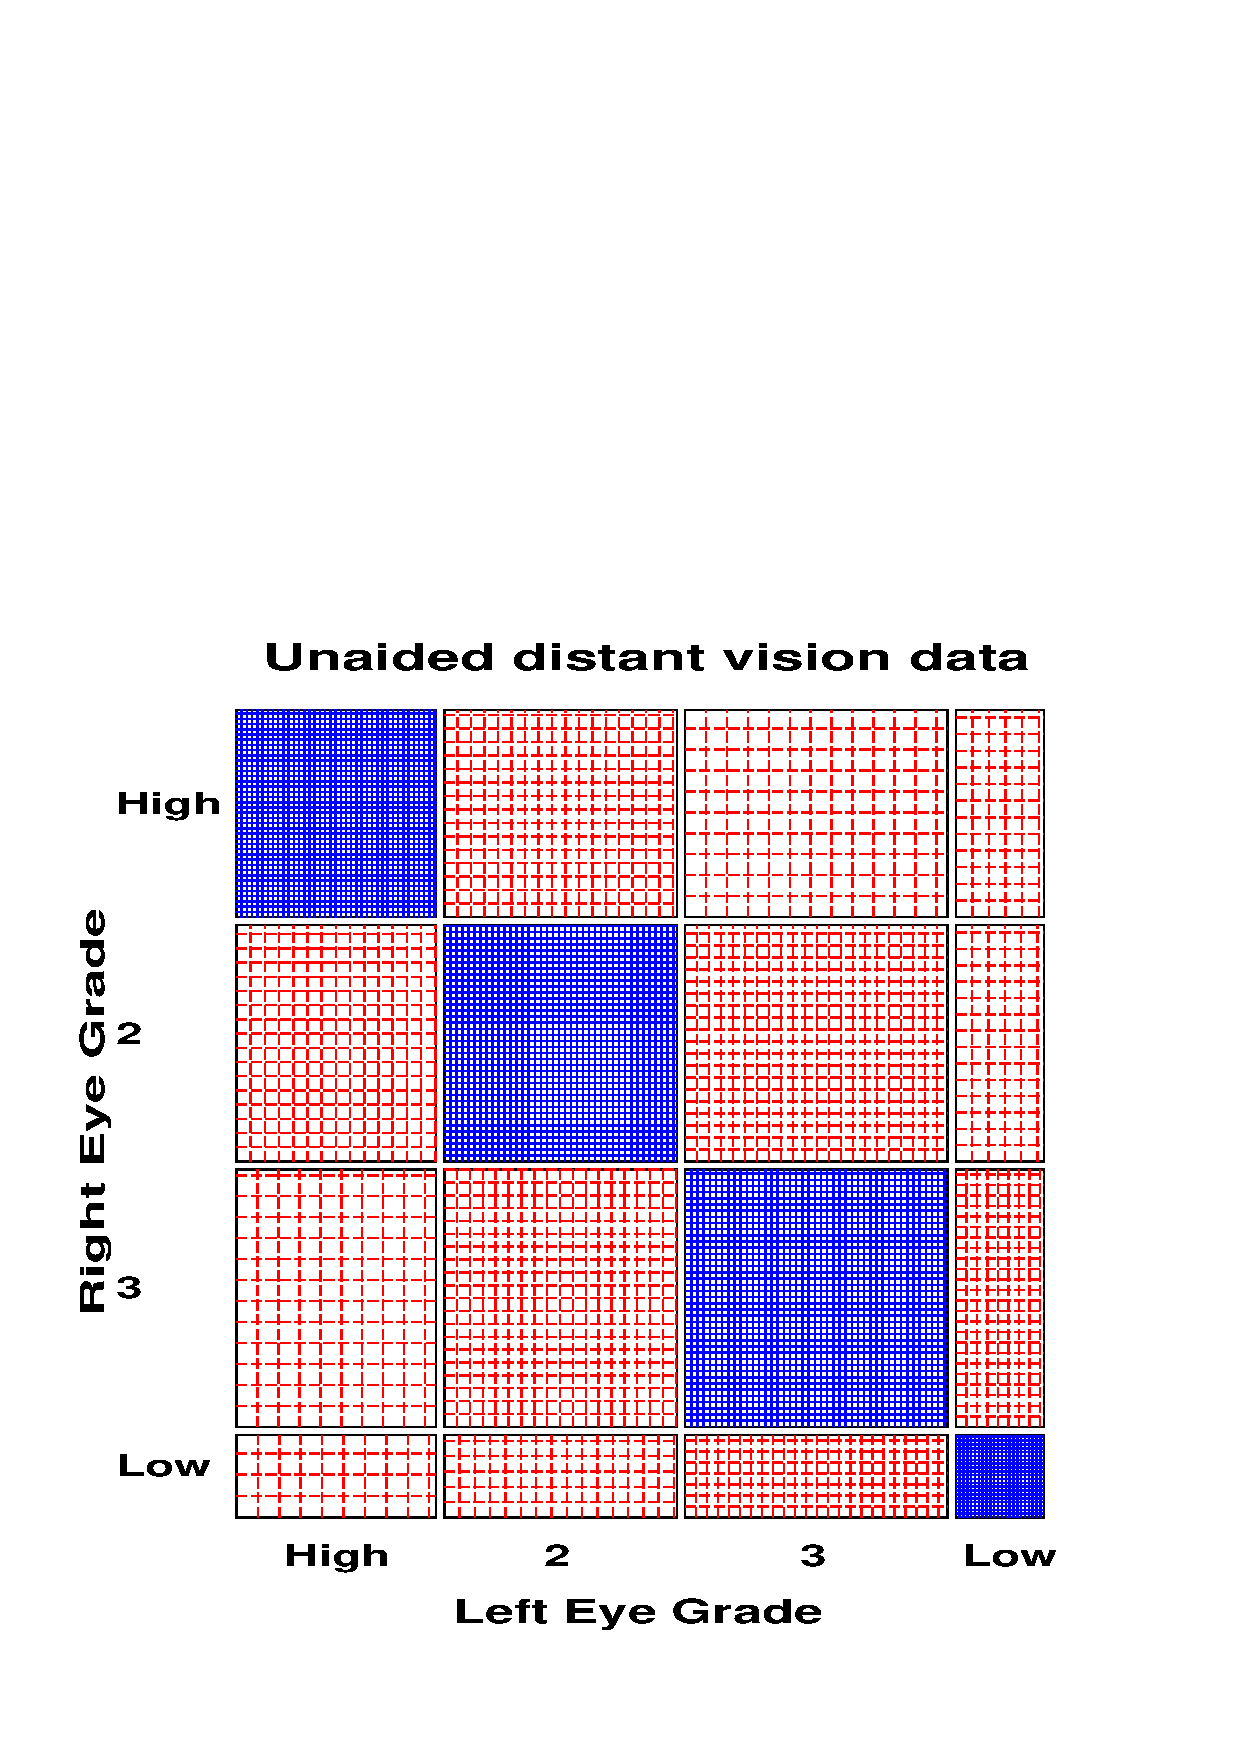
\includegraphics[width=1\linewidth,clip]{fig/sieve2}
  \end{minipage}%
 \hfill
 \begin{minipage}[c]{.33\textwidth}
  \includegraphics[width=1\linewidth,clip]{fig/mosaic3m1}
 \end{minipage}
  \rule{0.5pt}{4pt}\hrulefill\rule{0.5pt}{4pt} \\
	}
\date[VCD, 2012] % (optional)
{Short Course, 2012 \\
\small Web notes: \texttt{datavis.ca/courses/VCD/}}
% \\ SCS Short Course}

\subject{VCD}

% Delete this, if you do not want the table of contents to pop up at
% the beginning of each subsection:

\AtBeginSection[]
{
  \begin{frame}<beamer>
    \frametitle{Lecture outline}
    \tableofcontents[currentsection,currentsubsection,hideothersubsections]
  \end{frame}
}

%\includeonlylecture{Overview}
%\includeonlylecture{Two-way}
%\includeonlylecture{n-way}
%\includeonlylecture{Model}
\includeonlylecture{Polytomous}

\begin{document}

\begin{frame}[plain]
  \titlepage
\end{frame}

\lecture{Overview}{Overview}
\renewcommand{\FileName}{part1}
\part{Introduction}
\renewcommand{\FileName}{goals}

\begin{frame}
  \frametitle{Course goals}
  \begin{block}{Emphasis: visualization methods}<1->
     \begin{itemize}
      \item Basic ideas: categorical vs.\ quantitative data
      \item Some novel displays: sieve diagrams, fourfold displays, mosaic plots, ...
      \item Some that extend more familiar ideas to the categorical data setting.
     \end{itemize}
  \end{block}

  \begin{block}{Emphasis: theory $\Rightarrow$ practice}<2->
     \begin{itemize}
      \item Show \emph{what} can be done, in both SAS and R (most in SAS)
      \item Framework for \emph{thinking} about categorical data analysis in visual terms
      \item Provide software tools you can \emph{use}
     \end{itemize}
  \end{block}

  \begin{block}{What is included, and what is \textit{not}}<3->
     \begin{itemize}
      \item \emph{Some} description of statistical methods--- only as necessary
      \item \emph{Many} software examples--- only explained as necessary
      \item \emph{Too much} material--- some skipping may be required
     \end{itemize}   
  \end{block}

%   \begin{block}{What is \textit{not} included}
%      \begin{itemize}
%       \item 
%      \end{itemize}   
%   \end{block}
\end{frame}


\renewcommand{\FileName}{structure}

\begin{frame}
  \frametitle{Course structure, Parts 1--3}
  \begin{block}{1. Overview and introduction}<+->
     \begin{itemize}
      \item Categorical data? Graphics?
      \item Discrete distributions
      \item Testing association
     \end{itemize}
  \end{block}

  \begin{block}{2. Visualizing two-way and n-way tables}<+->
     \begin{itemize}
      \item 2 $\times 2$ tables; $r \times c$ tables: Fourfold \& sieve diagrams
      \item Observer agreement: Measures and graphs
      \item Correspondence analysis 
     \end{itemize}
  \end{block}

  \begin{block}{3. Mosaic displays and loglinear models}<+->
     \begin{itemize}
      \item $n$-way tables: graphs and models
      \item Mosaics software
      \item Structured tables 
     \end{itemize}   
  \end{block}
\end{frame}

\begin{frame}
  \frametitle{Course structure, Parts 4--5}
  \begin{block}{4. Logit models and logistic regression}<+->
     \begin{itemize}
      \item Logit models; logistic regression models
	  \item Effect plots
      \item Influence and diagnostic plots
     \end{itemize}   
  \end{block}
  \begin{block}{5. Polytomous response models}<+->
     \begin{itemize}
      \item Proportional odds models
	  \item Nested dichotomies
      \item Generalized logits
     \end{itemize}   
  \end{block}
\end{frame}


\section{Overview}

\subsection{What is categorical data?}
\section{What is categorical data?}\label{sec:intro-whatis}

A \emph{categorical variable} is one for which the possible measured
or assigned values
consist of a discrete set of categories.
Some typical examples are:
\begin{itemize*}
\item ``Gender'', with categories ``Male'', ``Female''.
\item ``Marital status'', with categories ``Never married'', ``Married'',
``Separated'', ``Divorced'', ``Widowed''.
\item ``Fielding position'' (in baseball), with categories
``Pitcher'', ``Catcher'', ``1st base'', ``2nd base'',  $\dots$, ``Left field''.
\item ``Side effects'' (in a pharmacological study), with categories
``None'', ``Skin rash'', ``Sleep disorder'', ``Anxiety'', $\dots$.
\item ``Political preference'', with categories ``Left'', ``Center'', ``Right''.
\item ``Treatment outcome'', with categories ``no improvement'', ``some
improvement'', or ``marked improvement''.
\item ``Age'', with categories ``0-9'', ``10-19'', ``20-29'', ``30-39'', 
$\dots$ .
\item ``Number of children'', with categories $0, 1, 2, \dots$ .
\end{itemize*}

As these examples suggest, categorical variables differ in the number of
categories: we often distingish 
\glossterm{binary variables} such as ``Gender''
from those with more than two categories (called \glossterm[polytomous]{polytomous variables}).
For example, \tabref{tab:berk220} gives data on 4526 applicants
to graduate departments at the University of California at Berkeley
in 1973, classified by two binary variables, gender and admission status.
\ixe{Berkeley admissions}
\begin{table}[tb]
\caption{Admissions to Berkeley graduate programs}
\label{tab:berk220}
 \begin{center}
\begin{tabular}{lrr|r}
\hline
  & Admitted & Rejected & Total  \\
\hline
 Males & 1198 & 1493 & 2691  \\
 Females & 557 & 1278 & 1835  \\
\hline
 Total & 1755 & 2771 & 4526  \\
\hline
\end{tabular}
\end{center}
\end{table}

Some categorical variables (``Political preference'', ``Treatment outcome'')
may have ordered categories (and are called \glossterm{ordinal}),
while other (\glossterm{nominal}) variables like ``Marital status''
have unordered categories.%
\footnote{An ordinal variable may be defined as one whose categories are
\emph{unambiguously} ordered along a \emph{single} underlying dimension.
Both marital status and fielding position may be weakly ordered, but
not on a single dimension, and not unambiguously.} 
For example, \tabref{tab:arthrit0} shows a $2 \times 2 \times 3$ table of 
ordered outcomes (``none'', ``some'' or ``marked'' improvement)
to an active treatment for rheumatoid
arthritis compared to a placebo for men and women.
\ixe{Arthritis treatment}
\begin{table}[htb]

\caption{Arthritis treatment data}\label{tab:arthrit0}
\begin{center}
\begin{tabular}{|ll|rrr|r|}
\hline
     &  & \multicolumn{3}{c|}{Improvement}            &  \\
\hline
   Treatment&  Sex    &None    &Some    &Marked  &  Total \\[1ex]
\hline
   Active   &  Female &      6 &      5 &     16 &     27 \\
            &  Male   &      7 &      2 &      5 &     14 \\ [0.5ex]
%\hline
   Placebo  &  Female &     19 &      7 &      6 &     32 \\
            &  Male   &     10 &      0 &      1 &     11 \\[1ex]
\hline
   Total    &         &     42 &     14 &     28 &     84 \\
\hline
\end{tabular}
\end{center}
\end{table}



Finally, such variables differ in the
fineness or level to which some underlying observation has been
categorized for a particular purpose.
From one point of view, \emph{all} data
may be considered categorical because the precision of measurement
is necessarily finite, or an inherently continuous variable may be recorded only to limited precision.   But this view is not helpful for the applied
researcher because it neglects the phrase ``for a particular purpose''.
Age, for example, might be treated as a quantitative variable in a study of
native language vocabulary, or as an ordered categorical variable in terms of
the efficacy or side-effects of treatment for depression, or even as a
binary variable (``child'' vs.\  ``adult'') in an analysis of survival following
an epidemic or natural disaster.


\subsection{Case form vs.\ Frequency form}
In many circumstances, data is recorded on each individual or experimental
unit.  Data in this form is called case data,
or data in \glossterm{case form}.
The data in \tabref{tab:arthrit0}, for example, were derived from
the individual data listed in \datref{dat:arthrit}.
Whether
or not the data variables, and the questions we ask call for
categorical or quantitative data analysis, we can always trace
any observation back to its individual identifier or data record
when the data are in case form.

Data in \glossterm{frequency form}, such as that shown in \tabref{tab:arthrit0},
has already been tabulated, by counting over the categories of the
table variables.  Data in frequency form may be analyzed by methods
for quantitative data if there is a quantitative response variable
(weighting each group by the cell frequency, with a \texttt{WEIGHT}
or \texttt{FREQ} statement).  Otherwise, such data are generally
best analyzed by methods for categorical data.
In either case, however, an observation in a \Dset\ in
frequency form refers
to all cases in the cell collectively, and cannot be identified individually.
Data in case form can always be reduced to frequency form,
but the reverse is rarely possible.

\subsection{Frequency data vs.\ Count data}
In many cases the observations represent the classifications of events or variables are 
recorded from \emph{operationally independent} experimental units or individuals, typically
a sample from some population.  The tabulated data may be called
\glossterm{frequency data}.  The data in \tabrefs{tab:berk220,tab:arthrit0}
are both examples of frequency data because each observation tabulated
comes from a different person.

However, if several events or variables are observed for the same units or individuals, those events are not
operationally independent, and it is useful to use the term 
\glossterm{count data} in this situation.  These terms (following
\citet{Lindsey:95}) are by no means standard, but
the distinction is often important, particularly in statistical
models for categorical data.  In a tabulation of the number of male
children within families (\tabref{tab:saxdata}), for example,
the number of male children in a given family would be a count variable,
taking values $0, 1, 2, \dots$.  The number of independent families with
a given number of male children is a frequency variable.
Count data also arise when we tabulate a sequence of events over time
or under different circumstances in a number of individuals.


\subsection{Univariate, bivariate, and multivariate data}
\tabref{tab:berk220} is an example of a bivariate (two-way) \ctab\
and \tabref{tab:arthrit0} classifies the observations by three variables.
Yet, we will see that the Berkeley admisssions data also recorded
the department to which potential students applied (giving a three-way
table), and in the arthritis data, the age of subjects was also
recorded.

Any \ctab, therefore records the marginal totals, summed over all
variables not represented in the table.
For data in case form, this means simply ignoring (or not recording)
one or more variables;  the ``observations'' remain the same.
Data in frequency form, however, result in smaller tables when
any variable is ignored;  the ``observations'' are the cells of
the \ctab.

In the limiting case, only one table variable may be recorded or
available, giving the categorical equivalent of univariate data.
For example, \tabref{tab:saxdata} gives data on the distribution
of the number of male children in families with 12 children
discussed in \exref{ex:saxony1}.
These data were part of a large tabulation of the sex distribution
of families in Saxony in the 19th century, but the data in \tabref{tab:saxdata}
have only one discrete classification variable, number of males.
Without further information, the only statistical questions concern
the form of the distribution.
We discuss methods for fitting and graphing such discrete distributions
in \chref{ch:discrete}.
The remaining chapters relate to bivariate and multivariate data.
\ixe{Families in Saxony}
\begin{table}[htb]
 \caption{Number of Males in 6115 Saxony Families of Size 12}\label{tab:saxdata}
 \begin{center}
 \begin{tabular}{l|rrrrrrrrrrrrr}
  \hline
  Males & 0 & 1 & 2 & 3 & 4 & 5 & 6 & 7 & 8 & 9 & 10 & 11 & 12 \\ 
  Families & ~~~3 & ~~24 & ~104 & ~286 & ~670 & 1,033 & 1,343 & 1,112 & ~829 & ~478 & 181 & ~~45 & ~~~7 \\ 
  \hline
 \end{tabular}
 \end{center}
\end{table}


\subsection{Explanatory vs.\ Response variables}
\ix{variable!response \~|(}
Many statistical models make a distinction between \emph{response}
(or \emph{dependent}, or \emph{criterion})
variables and
\emph{explanatory}
(or \emph{independent}, or \emph{predictor})
variables.
In the standard (classical) linear models for regression and analysis of variance
(ANOVA), for instance, we treat one (or more) variables as responses,
to be explained by the other, explanatory variables.
The explanatory variables may be quantitative or categorical
(e.g., \texttt{CLASS} variables), but
this affects only the details of how the model is specified for
\PROC{GLM} or \PROC{REG}.
The response variable, treatment outcome, for example, must be
considered quantitative,  and the model attempts to describe how the
\emph{mean} of the distribution of responses changes with the values
or levels of the explanatory variables, such as age or gender.


When the response variable is categorical, however, the standard linear
models do not apply, because they assume a normal (Gaussian) distribution
for the model residuals.  For example, in \tabref{tab:arthrit0} 
the response is Improvement, and even if numerical scores were assigned
to the categories ``none'', ``some'', ``marked'', it may be unlikely
that the assumptions of the classical linear models could be met.

Hence, a categorical \emph{response variable} generally requires analysis
using methods for categorical data, but categorical explanatory variables
may be readily handled by either method.
\ix{variable!response \~|)}

\subsection{Methods}
\renewcommand{\FileName}{overview}

\begin{comment}
\begin{frame}[allowframebreaks]
	\frametitle{Categorical Data Analysis: Methods}
Methods of analysis for categorical data fall into two main categories:

\begin{itemize}

\item {\bfseries\large Non-parametric, randomization-based methods}

    \begin{itemize}
    \item make minimal assumptions
    \item useful for hypothesis-testing 
    \item SAS: \PROC{FREQ}; SPSS: Crosstabs
        \begin{itemize*}
        \item Pearson Chi-square
        \item \IX{Fisher's exact test} (for small expected
                frequencies)
        \item Mantel-Haenszel tests (ordered categories: test
                for \emph{linear} association)
        \end{itemize*}
	\item R: \func{chisq.test}, \func{mantelhaen.test}, ...
    \end{itemize}

\framebreak
\item {\bfseries\large Model-based methods}

    \begin{itemize}
    \item Must assume random sample (possibly stratified)
    \item Useful for estimation purposes (std. errors, confidence intervals)
    \item Greater flexibility; fitting specialized models 
		\begin{itemize*}
		 \item Symmetry, quasi-symmetry, structured associations for square tables
		 \item Models for ordinal variables
		\end{itemize*}

    \item More suitable for multi-way tables
    \item SAS: \PROC{LOGISTIC}, \proc{CATMOD}, \proc{GENMOD} , \proc{INSIGHT} (Fit YX)
        \begin{itemize*}
        \item estimate standard errors, covariances for model parameters
        \item confidence intervals for parameters, predicted Pr\{response\}
        \end{itemize*}
    \item R: \func{glm} family, \pkg{car}, \pkg{gnm}, ...
	\item SPSS: Hiloglinear, Loglinear, Generalized linear models
    \end{itemize}

\end{itemize}
\end{frame}
\end{comment}

\begin{frame}
	\frametitle{Categorical data: Analysis methods}
Methods of analysis for categorical data fall into two main categories:

\begin{block}{\large\bfseries Non-parametric, randomization-based methods}
    \begin{itemize}
    \item Make minimal assumptions
    \item Useful for \alert{hypothesis-testing}: Are A and B associated?
    \item Mostly for \alert{two-way} tables (possibly stratified)
    \item SAS: \PROC{FREQ}
        \begin{itemize*}
        \item Pearson Chi-square
        \item \IX{Fisher's exact test} (for small expected frequencies)
        \item Mantel-Haenszel tests (ordered categories: test for \emph{linear} association)
        \end{itemize*}
	\item R: \func{chisq.test}, \func{mantelhaen.test}, ...
	\item SPSS: Crosstabs
    \end{itemize}
\end{block}
\end{frame}

\begin{frame}
	\frametitle{Categorical data: Analysis methods}

\begin{block}{\large\bfseries Model-based methods}
    \begin{itemize}
    \item Must assume random sample (possibly stratified)
    \item Useful for \alert{estimation} purposes: Size of effects (std. errors, confidence intervals)
    \item More suitable for \alert{multi-way} tables
    \item Greater flexibility; fitting specialized models
		\begin{itemize*}
		 \item Symmetry, quasi-symmetry, structured associations for square tables
		 \item Models for ordinal variables
		\end{itemize*}
    \item SAS: \PROC{LOGISTIC}, \proc{CATMOD}, \proc{GENMOD} , \proc{INSIGHT} (Fit YX)
        \begin{itemize*}
        \item estimate standard errors, covariances for model parameters
        \item confidence intervals for parameters, predicted Pr\{response\}
        \end{itemize*}
    \item R: \func{glm} family, \pkg{car}, \pkg{gnm}, ...
	\item SPSS: Hiloglinear, Loglinear, Generalized linear models
    \end{itemize}
\end{block}
\end{frame}

\begin{frame}[label=resp-assoc]
 \frametitle{Categorical data: Response vs. Association models}
  \begin{block}{\large\bfseries Response models}<1->
   \begin{itemize}
    \item Sometimes, one variable is a  natural discrete response.
    \item Q: How does the response relate to explanatory variables?
		\begin{itemize*}
		 \item Admit $\sim$ Gender + Dept
         \item Party $\sim$ Age + Education + Urban
		\end{itemize*}
    \item[$\Rightarrow$] Logit models, logististic regression, generalized linear models
   \end{itemize}
  \end{block}

  \begin{block}{\large\bfseries Association models}<2->
   \begin{itemize}
    \item Sometimes, the main interest is just \alert{association}
    \item Q: Which variables are associated, and \alert{how}?
		\begin{itemize*}
		 \item Berkeley data: [Admit Gender]?  [Admit Dept]? [Gender Dept]
         \item Hair-eye data: [Hair Eye]? [Hair Sex]? [Eye, Sex]
		\end{itemize*}
    \item[$\Rightarrow$] Loglinear models
   \end{itemize}
  \end{block}

   This is similar to the distinction between regression/ANOVA vs.\
   correlation and factor analysis
\end{frame}

\subsection{Graphical methods}
\begin{frame}
  \frametitle{Graphical methods: Tables and Graphs}

  \begin{namedQuote}{Albert Einstein}
  If I can't picture it, I can't understand it.
  \end{namedQuote}
%  \begin{namedQuote}{Yogi Berra}
%  You can see a lot, just by looking.
%  \end{namedQuote}
  \begin{namedQuote}{Farquhar \& Farquhar, 1891}
  Getting information from a table is like extracting sunlight
  from a cucumber.
  \end{namedQuote}


  \begin{block}{\large\bfseries Tables vs.\ Graphs}
      \begin{itemize}
      \item Tables are best suited for \emph{look-up} and calculation---  
		\begin{itemize*}
		 \item read off exact numbers
		 \item additional calculations (e.g., \% change)
		\end{itemize*}

	  \item Graphs are better for:
	  \begin{itemize*}
	      \item showing \emph{patterns, trends, anomalies}, 
	      \item making \emph{comparisons}
	      \item seeing the \emph{unexpected}!
	  \end{itemize*}
	  \item Visual presentation as \emph{communication}: 
	  \begin{itemize*}
			\item what do you want to say or show?
			\item design graphs and tables to 'speak to the eyes'
	  \end{itemize*}
	  \end{itemize}
  \end{block}
\end{frame}


\begin{frame}
\frametitle{Graphical methods: Quantitative data}
Quantitative data (amounts) are  naturally displayed in terms of
	\(
	\mbox{\bf magnitude} \sim \mbox{\bf position along a scale}
	\)

\vspace{1ex}
%% two subfig side-by-side
 \begin{minipage}[t]{.45\textwidth}
  \includegraphics[width=1\linewidth,clip]{fig/lm-income-experience}
  \\ \centering Scatterplot of Income vs. Experience
 \end{minipage}%
 \hfill
 \begin{minipage}[t]{.45\textwidth}
  \includegraphics[width=1\linewidth,clip]{fig/lm-income-gender}
  \\ \centering Boxplot of Income by Gender
 \end{minipage}

\end{frame}

\begin{frame}
\frametitle{Graphical methods: Categorical data}
Frequency data (counts) are more naturally displayed in terms of
	\(
	\mbox{\bf count} \sim \mbox{\bf area}
	\)
	\citep{Friendly:95}

%% two subfig side-by-side
 \begin{minipage}[t]{.45\textwidth}
  \includegraphics[width=1\linewidth,clip]{fig/pie2x2g}
  \\ \centering Fourfold display for 2$\times$2 table
 \end{minipage}%
 \hfill
 \begin{minipage}[t]{.45\textwidth}
  \includegraphics[width=1\linewidth,clip]{fig/mosaic9a3f}
  \\ \centering Mosaic plot for 3-way table
 \end{minipage}

\end{frame}

\begin{frame}

  \begin{itemize}
	\item{\large\bfseries Principles of Graphical Displays}
      \begin{itemize*}
	  \item {\bfseries Effect ordering} \citep{FriendlyKwan:02:effect}--- In tables and graphs, sort unordered factors
	  according to the effects you want to see/show.
	    \vspace{1ex}
		\begin{center}
		\includegraphics[width=.9\textwidth,clip]{fig/corrgram2}
		\end{center}
``Corrgrams: Exploratory displays for correlation matrices'' \citep{Friendly:02:corrgram}
      \end{itemize*}
  \end{itemize}
\end{frame}

\begin{frame}[t]
  \begin{itemize*}
	\item Effect ordering and high-lighting for tables \citep{Friendly:00:mdarray}
%\makeatletter\slidebox@restore\makeatother
	\input{tab/haireye-eff-beamer}
  \end{itemize*}	
\end{frame}

\begin{frame}
  \begin{itemize*}
	  \item {\bfseries Comparisons}--- Make visual comparisons easy
    	\begin{itemize*}
		\item Visual grouping--- connect with lines, make key comparisons contiguous
		\item Baselines--- compare \emph{data} to \emph{model} against a line, preferably horizontal
		\end{itemize*}
  \end{itemize*}
	  \vspace{1ex}
	  \begin{center}
	  \includegraphics[width=.9\textwidth,clip]{fig/madfit2} \\
      \begin{minipage}{.45\linewidth}
      \centering Standard histogram with fit  
      \end{minipage}
		\hfill 
      \begin{minipage}{.45\linewidth}
      \centering Suspended rootogram 
      \end{minipage}
	  \end{center}
\end{frame}

\begin{frame}

  \begin{itemize}
	  \item {\bfseries Small multiples}--- combine stratified graphs into coherent displays \citep{Tufte:83}
    	\begin{itemize*}
		\item e.g., scatterplot matrix for quantitative data: all pairwise scatterplots
		\end{itemize*}
	  \vspace{1ex}
	  \begin{center}
	  \includegraphics[width=.6\textwidth,clip]{fig/prestige22}
	  \end{center}
  \end{itemize}
\end{frame}

\begin{frame}
    \begin{itemize*}
		\item e.g., mosaic matrix for quantitative data: all pairwise mosaic plots
	\end{itemize*}
	  \vspace{1ex}
	  \begin{center}
	  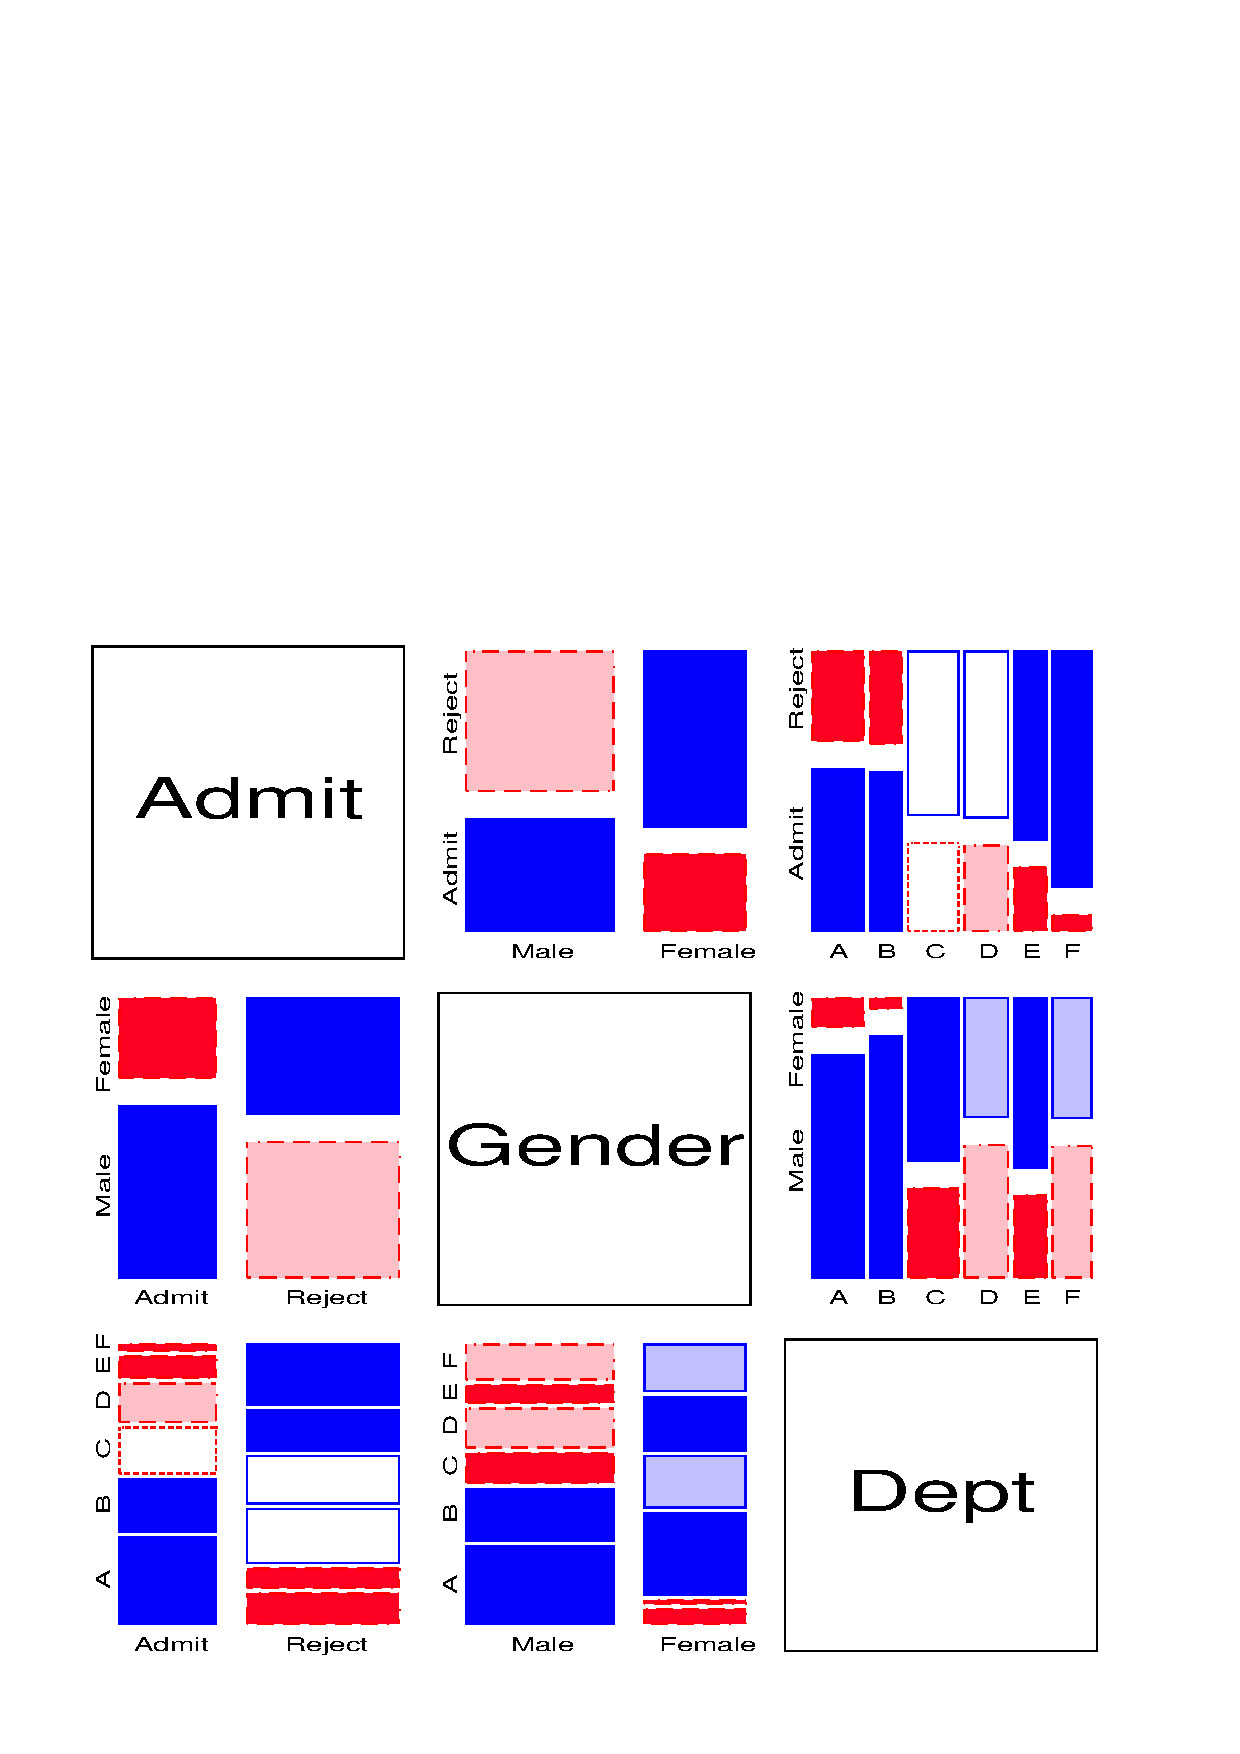
\includegraphics[width=.6\textwidth,clip]{fig/mosmat9a}
	  \end{center}
\end{frame}

\begin{frame}
 \frametitle{Graphical methods: Categorical data}
  \begin{block}{\large\bfseries Exploratory methods}<1->
      \begin{itemize*}
	  \item Minimal assumptions (like non-parametric methods)
	  \item Show the \emph{data}, not just \emph{summaries} 
	  \item Help detect \emph{patterns, trends, anomalies}, suggest hypotheses
	  \end{itemize*}
   \end{block}

	\begin{block}{\large\bfseries Plots for model-based methods}<2->
      \begin{itemize*}
	  \item Residual plots - departures from model, omitted terms, ...
	  \item Effect plots - estimated probabilities of response or log odds 
	  \item Diagnostic plots - influence, violation of assumptions
	  \end{itemize*}
   \end{block}

	\begin{block}{\large\bfseries Goals}<3->
      \begin{itemize*}
	  \item \emph{VCD} and R \pkg{vcd} - Make these methods \emph{available} and \emph{accessible} in SAS \& R
	  \item {\bf Practical power = Statistical power \(\times\) Probability of Use}
	  \item Today's goal:  take-home knowledge
	  \item Tomorrow's goal: dynamic, interactive graphics for categorical data 
	  \end{itemize*}
   \end{block}
\end{frame}

\endinput

% slide template
\begin{frame}
  \frametitle{}
  \begin{itemize}
	\item{\large\bfseries }
      \begin{itemize*}
	  \item 
    	\begin{itemize*}
		\item 
		\item 
		\end{itemize*}
	  \item 
	  \end{itemize*}
	\item{\large\bfseries }
	\item{\large\bfseries }
  \end{itemize}
\end{frame}


\subsection{Software: SAS}
\renewcommand{\FileName}{vcdmacros}

\begin{frame}
\frametitle{\VCD\ Macros \& \IML\ programs}
\begin{itemize}
\item Macros, \Dset{}s available at \url{datavis.ca/vcd/}
\end{itemize}

\begin{block}{Discrete distributions}<1->
\begin{proglist*}
	\item[DISTPLOT] Plots for discrete distributions 
	\item[GOODFIT] Goodness-of-fit for discrete distributions 
	\item[ORDPLOT] Ord plot for discrete distributions 
	\item[POISPLOT] Poissonness plot 
	\item[ROOTGRAM] Hanging rootograms 
\end{proglist*}
\end{block}

\begin{block}{Two-way and $n$-way tables}<2->
\begin{proglist*}
	\item[AGREEPLOT] Observer agreement chart 
	\item[CORRESP] Plot \PROC{CORRESP} results 
	\item[FFOLD] Fourfold displays for $2 \times 2 \times k$ tables
%	\item[FOURFOLD] Fourfold displays for $2 \times 2 \times k$ tables (\IML)
	\item[SIEVEPLOT] Sieve diagrams
	\item[MOSAIC] Mosaic displays 
%	\item[MOSAICS] \IML{} modules for mosaic displays 
	\item[MOSMAT] Mosaic matrices 
	\item[TABLE] Construct a grouped frequency table, with recoding 
	\item[TRIPLOT] Trilinear plots for $n \times 3$ tables 
\end{proglist*}
\end{block}
\end{frame}

\begin{frame}
\begin{block}{Model-based methods}<1->
\begin{proglist*}
	\item[ADDVAR] Added variable plots for logistic regression 
	\item[CATPLOT] Plot results from \PROC{CATMOD}
	\item[HALFNORM] Half-normal plots for generalized linear models 
	\item[INFLGLIM] Influence plots for generalized linear models 
	\item[INFLOGIS] Influence plots for logistic regression 
	\item[LOGODDS] Plot empirical logits and probabilities for binary data 
	\item[POWERLOG] Power calculations for logistic regression 
%	\item[POWERRxC] Power calculations for two-way frequency table 
%	\item[POWER2x2] Power calculations for a $2\times 2$ table 
%	\item[ROBUST] Robust fitting for linear models 
%	\item[TWOWAY] Two-way table display 
\end{proglist*}
\end{block}

\begin{block}{Utility macros}<2->
\begin{proglist}
	\item[DUMMY] Create dummy variables 
	\item[LAGS] Calculate lagged frequencies for sequential analysis 
	\item[PANELS] Arrange multiple plots in a panelled display 
	\item[SORT] Sort a dataset by the value of a statistic or formatted value 
	\item[Utility] Graphics utility macros:
	\pname{bars},
	\pname{equate},
	\pname{gdispla},
	\pname{gensym},
	\pname{gskip},
	\pname{label},
	\pname{points},
	\pname{pscale}
\end{proglist}
\end{block}
\VCD\ Archive (\texttt{vcdprog.zip}) available at:
\url{http://datavis.ca/courses/VCD/vcdprog.zip}
\end{frame}


\subsection{Software: R}
\renewcommand{\FileName}{vcdpackage}

\begin{frame}
\frametitle{R software and the \texttt{vcd} package}
\begin{itemize}
\item R software and the \texttt{vcd} package, 
available at \url{www.r-project.org}
\end{itemize}

\begin{block}{Discrete distributions}<1->
\begin{proglist}
	\item[distplot] Plots for discrete distributions 
	\item[goodfit] Goodness-of-fit for discrete distributions 
	\item[ordplot] Ord plot for discrete distributions 
	\item[poisplot] Poissonness plot 
	\item[rootgram] Hanging rootograms 
\end{proglist}
\end{block}

\begin{block}{Two-way and $n$-way tables}<2->
\begin{proglist}
	\item[agreementplot] Observer agreement chart 
	\item[fourfold] Fourfold displays for $2 \times 2 \times k$ tables 
	\item[sieve] Sieve diagrams
	\item[mosaic] Mosaic displays 
	\item[pairs.table] Matrix of pairwise association displays 
	\item[structable] Manipulate high-dimensional contingency tables 
	\item[triplot] Trilinear plots for $n \times 3$ tables 
\end{proglist}
\end{block}
\end{frame}

\begin{frame}[t]
\frametitle{R software: Other packages}
\begin{block}{Model-based methods}
\begin{proglist}
	\item[glm] Fitting generalized linear models 
	\item[gnm] Fitting generalized \emph{non-linear} models, e.g., RC(1) model
	\item[loglm] MASS package: Fitting loglinear models 
	\item[Rcmdr] Menu-driven package for statistical analysis and graphics
	\item[car] Graphics and extensions of generalized linear models 
	\item[effects] Effects plots for generalized linear models 
\end{proglist}
\end{block}
%\begin{itemize}
%\item Additional material in the  \texttt{vcdExtra} package, 
%available at \url{http://R-Forge.R-Project.org/vcdextra}
%\end{itemize}
\begin{block}{vcdExtra package}
\begin{proglist}
    \item[vcd-tutorial] Vignette on working with categorical data and the vcd package
	\item[mosaic.glm] mosaic displays for GLMs and GNMs
	\item[mosaic3d] 3D mosaic displays 
	\item[glmlist] Methods for working with lists of models
\end{proglist}
\end{block}

\end{frame}


\section{Discrete distributions}
%\subsection{Using SAS}
\renewcommand{\FileName}{discrete}
\begin{comment}
\begin{frame}
  \frametitle{Discrete distributions}  
  \begin{itemize}
	\item {\large\bfseries Counts of occurrences:} accidents, words in text, 
	blood cells with some characteristic.
	\item{\large\bfseries Data:} Basic outcome value, \(k \,  , \,  k = 0 , 1, \dots\),
	and number of observations, \(n_k\), with that value.
	\item {\large\bfseries Example:} \emph{Federalist Papers}--- disputed authorship 
      \begin{itemize*}
	  \item 77 essays by Hamilton, Jay \& Madison: persuade NY voters to ratify Constitution, all
	  signed with pseudonym (``Publius'')
	  \item 65 known, 12 disputed (H \& M both claimed sole authorship)
	  \item \citet{MostellerWallace:84}: Analysis of frequency distributions of key ``marker'' words:
\emph{from}, \emph{may}, \emph{whilst}, $\dots$.
	  \item For each word, fit probability model (Poisson, NegBin)
$\rightarrow (\beta_1, \beta_2, \cdots) \longrightarrow $
log Odds (Hamilton vs. Madison)
	  \end{itemize*}
  \end{itemize}

  %\begin{table}[htb]
% \caption{Number of occurrences ($k$) and number of blocks of text ($n_k$) of the word \emph{may} in 
%essays written by  Madison}\label{tab:madison}
 \begin{center}
 \begin{tabular}{l|rrrrrrr}
  \hline
  Occurrences ($k$)   &   0 &  1 &  2 & 3 & 4 & 5 & 6 \\ 
      Blocks ($n_k$)  & 156 & 63 & 29 & 8 & 4 & 1 & 1 \\ 
  \hline
 \end{tabular}
 \end{center}
%\end{table}

\end{frame}
\end{comment}

\begin{frame}
  \frametitle{Discrete distributions}  
  \begin{itemize}
	\item {\large\bfseries Counts of occurrences:} accidents, words in text, 
	blood cells with some characteristic.
	\item{\large\bfseries Data:} Basic outcome value, \(k \,  , \,  k = 0 , 1, \dots\),
	and number of observations, \(n_k\), with that value.
	\item {\large\bfseries Example:} distributions of key ``marker''
	words: \emph{from}, \emph{may}, \emph{whilst}, $\dots$ in \emph{Federalist Papers}
	by James Madison, e.g., blocks of 200 words with  \emph{may}:

  %\begin{table}[htb]
% \caption{Number of occurrences ($k$) and number of blocks of text ($n_k$) of the word \emph{may} in 
%essays written by  Madison}\label{tab:madison}
 \begin{center}
 \begin{tabular}{l|rrrrrrr}
  \hline
  Occurrences ($k$)   &   0 &  1 &  2 & 3 & 4 & 5 & 6 \\ 
      Blocks ($n_k$)  & 156 & 63 & 29 & 8 & 4 & 1 & 1 \\ 
  \hline
 \end{tabular}
 \end{center}
%\end{table}


	\item {\large\bfseries Example:} Saxony
	families with 12 children having $k=0, 1, \dots 12$ sons.
  \end{itemize}
	
%\scalebox{.9}{%
%Unequal number of columns: 14 13
%\begin{table}[htb]
% \caption{Number of males in N=6115 Saxony families with 12 children}\label{tab:saxony}
 \begin{center}
 \setlength{\tabcolsep}{3pt}
 \begin{tabular}{l|rrrrrrrrrrrrr}
  \hline
  $k$ & 0 & 1 & 2 & 3 & 4 & 5 & 6 & 7 & 8 & 9 & 10 & 11 & 12 \\ 
  \hline
  $n_k$ & 3 & 24 & 104 & 286 & 670 & 1033 & 1343 & 1112 & 829 & 478 & 181 & 45 & 7 \\ 
  \hline
 \end{tabular}
 \end{center}
%\end{table}

%}
\end{frame}

\begin{frame}
  \frametitle{Discrete distributions}  

  \begin{block}{\large\bfseries Questions:}<1->
  	 \begin{itemize*}
  	 \item What process gave rise to the distribution?
  	 \item Form of distribution: uniform, binomial,
  	  Poisson, negative binomial, geometric, etc.?
  	 \item Estimate parameters
  	 \item Visualize goodness of fit
  	 \end{itemize*}
   \end{block}
  \begin{exampleblock}{\large\bfseries For example:}<2->
  	 \begin{itemize*}
  	 \item \emph{Federalist Papers:}  might expect a Poisson($\lambda$) distribution.
  	 \item \emph{Families in Saxony:}  might expect a Bin($n, p$) distribution 
  	 with $n=12$. Perhaps $p=0.5$ as well.
  	 \end{itemize*}
   \end{exampleblock}

\end{frame}

\begin{frame}
  \frametitle{Discrete distributions}  

  \begin{block}{\large\bfseries Lack of fit:}
	 \begin{itemize*}
     \item Lack of fit tells us something about the process giving rise to the data
     \item Poisson:  assumes constant small probability of the basic event
     \item Binomial: assumes constant probability and independent trials   
	 \end{itemize*}
  \end{block}

  \begin{exampleblock}{\large\bfseries Motivation:}
	 \begin{itemize*}
	   \item Models for more complex categorical data often use these basic discrete distributions
	   \item Binomial (with predictors) $\rightarrow$ logistic regression
	   \item Poisson (with predictors) $\rightarrow$ poisson regression, \loglin\ models 
	   \item $\Rightarrow$ many of these are special cases of \emph{generalized linear models}
	 \end{itemize*}

   \end{exampleblock}

\end{frame}

\subsection{Using SAS}
\begin{frame}
  \frametitle{Fitting and graphing discrete distributions}
  \begin{block}
      \VCD\ methods to fit, visualize, and diagnose discrete distributions:
  \end{block}

  \begin{itemize}
	\item{\large\bfseries Fitting:} \macro{GOODFIT} fits uniform, binomial,
 Poisson, negative binomial, geometric,  logarithmic series
 distributions (or any specified multinomial)

	\item{\large\bfseries Hanging rootograms:} Sensitively assess departure between Observed, Fitted
counts (\macro{ROOTGRAM})
	\item{\large\bfseries Ord plots:} Diagnose form of a discrete distribution (\macro{ORDPLOT})
	\item{\large\bfseries Poissonness plots:} Robust fitting and diagnostic plots for Poisson
(\macro{POISPLOT})
	\item{\large\bfseries Robust distribution plots} (\macro{DISTPLOT})
  \end{itemize}
\end{frame}

\subsection{Using SAS macros}
\begin{frame}[fragile]
  \frametitle{Sidebar: Using SAS macros}
  \begin{itemize}
    \item SAS macros are high-level, general programs consisting of a series of
	\texttt{DATA} steps and \texttt{PROC} steps.
	\item Keyword arguments substitute your data names, variable names, and
	options for the named macro parameters.
	\item Use as:
\begin{Code}
  %macname(data=dataset, var=variables, ...);
\end{Code}
	\item Most arguments have default values (e.g., \texttt{data=\_last\_})
	\item All \VCD\ macros have internal and online documentation,
	\url{http://datavis.ca/sasmac/}
	\item Macros can be installed in directories automatically searched by SAS.
	Put the following \texttt{options} statement in your \texttt{AUTOEXEC.SAS} file:
\begin{verbatim}
  options sasautos=('c:\sasuser\macros' sasautos);
\end{verbatim}

  \end{itemize}
\end{frame}

\begin{frame}[fragile]
  \frametitle{Sidebar: Using SAS macros}

E.g., the \macro{GOODFIT} is defined with the following arguments:
\vspace{1.5ex}
\begin{Input}[fontsize=\footnotesize,label=\fbox{$\cdots$ \texttt{goodfit.sas} $\cdots$},baselinestretch=0.8]
%macro goodfit(
  data=_last_,    \sascomment{/* name of the input data set             */}
  var=,           \sascomment{/* analysis variable (basic count)        */}
  freq=,          \sascomment{/* frequency variable                     */}
  dist=,          \sascomment{/* name of distribution to be fit         */}
  parm=,          \sascomment{/* required distribution parameters?      */}
  sumat=100000,   \sascomment{/* sum probs. and fitted values here      */}
  format=,        \sascomment{/* format for ungrouped analysis variable */}
  out=fit,        \sascomment{/* output fit data set                    */}
  outstat=stats); \sascomment{/* output statistics data set             */}
\end{Input}
Typical use:
\begin{Input}
%goodfit(data=madison, \sascomment{/* data set       */} 
    var=count,         \sascomment{/* count variable */}
    freq=blocks, 
    dist=poisson);
\end{Input}

\end{frame}

\subsection{Fitting discrete distributions} 
\begin{frame}
\frametitle{Fitting discrete distributions}
  \begin{itemize}
   \item {\large\bfseries Distributions:}
	 \begin{itemize*}
	   \item Poisson, $p(k) = e^{-\lambda }\lambda ^k/k!$
	   \item Binomial, $p(k) = \binom{n}{k} p^k(1-p)^{n-k}$
	   \item Negative binomial, $p(k) = \binom{n+k-1}{k}p^n(1-p)^k$
	   \item Geometric, $p(k) = p(1-p)^k$
	   \item Logarithmic series,  $p(k) = \theta ^k/[-k\log (1-\theta )]$
	 \end{itemize*}
  \item {\large\bfseries Estimate parameter(s):}
	 \begin{itemize*}
	   \item Poisson, $\hat\lambda = \sum k n_k / \sum n_k$ = mean
	   \item Binomial, $\hat p = \sum k n_k / (n \sum n_k)$ = mean / n
	 \end{itemize*}
  \item {\large\bfseries Goodness of fit:}
  \[
  \chi^2 = \sum_{k=1}^K \:
  \frac{{ ( n_k - N \hat{p}_k ) }^2}
  { N \hat{p}_k }  \sim \chi^2_{( K-1 )}
  \]
where \(\hat{p}_k\) is the estimated probability of each basic count,
under the hypothesis that the data follows the chosen distribution.
  \end{itemize}
\end{frame}

\begin{frame}[fragile]

\frametitle{\macrot{GOODFIT}: Fitting discrete distributions}
  \begin{itemize}
  \item \macro{GOODFIT} fits uniform, binomial,
   Poisson, negative binomial, geometric,  logarithmic series
   distributions (or any specified multinomial)
  \item E.g., Try fitting Poisson model
\end{itemize}

\vspace{1.5ex}
\begin{Input}[fontsize=\small,label=\fbox{\texttt{madfit.sas}},baselinestretch=0.8]
title "Instances of 'may' in Federalist papers";
data madison;
   input count blocks;
   label count='Number of Occurrences'
         blocks='Blocks of Text';
datalines;
  0    156
  1     63
  2     29
  3      8
  4      4
  5      1
  6      1
;
 %goodfit(data=madison, var=count, freq=blocks,  
      \sasemph{dist=poisson});
\end{Input}

\end{frame}

\begin{frame}[fragile]
\frametitle{Fitting discrete distributions}
The \macro{GOODFIT} gives a table of observed and fitted frequencies,
Pearson $\chi^2$ residuals (\texttt{CHI}) and likelihood-ratio deviance 
residuals (\texttt{DEV}).

\begin{Output}[gobble=2,fontsize=\footnotesize]
              Instances of 'may' in Federalist papers
 
   COUNT    BLOCKS      PHAT         EXP       CHI         DEV
 
     0        156     0.51867    135.891     1.72499     6.56171
     1         63     0.34050     89.211    -2.77509    -6.62056
     2         29     0.11177     29.283    -0.05231    -0.75056
     3          8     0.02446      6.408     0.62890     1.88423
     4          4     0.00401      1.052     2.87493     3.26912
     5          1     0.00053      0.138     2.31948     1.98992
     6          1     0.00006      0.015     8.01267     2.89568
            ======    =======    =======
              262     0.99999    261.998
\end{Output}
\end{frame}

\begin{frame}[fragile]
\frametitle{Fitting discrete distributions}
In addition, it provides the overall goodness-of-fit tests:
\begin{Output}[gobble=7]
         Goodness-of-fit test for data set MADISON
 
         Analysis variable:       COUNT Number of Occurrences
         Distribution:            POISSON
         Estimated Parameters:    lambda = 0.6565
 
         Pearson chi-square    = 88.92304707
         Prob > chi-square     = 0
 
         Likelihood ratio G2   = 25.243121314
         Prob > chi-square     = \sasemph{0.0001250511}
 
         Degrees of freedom    = 5
\end{Output}
The poisson model does not fit!  Why?
\end{frame}

\begin{frame}[fragile]

  \frametitle{What's wrong with histograms?}
  \begin{itemize}
  \item Discrete distributions often graphed as histograms, with a 
  theoretical fitted distribution superimposed.
%  \item E.g., Try fitting Poisson model

  \begin{Code}
   %goodfit(data=madison, var=count, freq=blocks,  
      \sasemph{dist=poisson});
  \end{Code}

  \end{itemize}

 \begin{minipage}[c]{.49\dispwidth}
  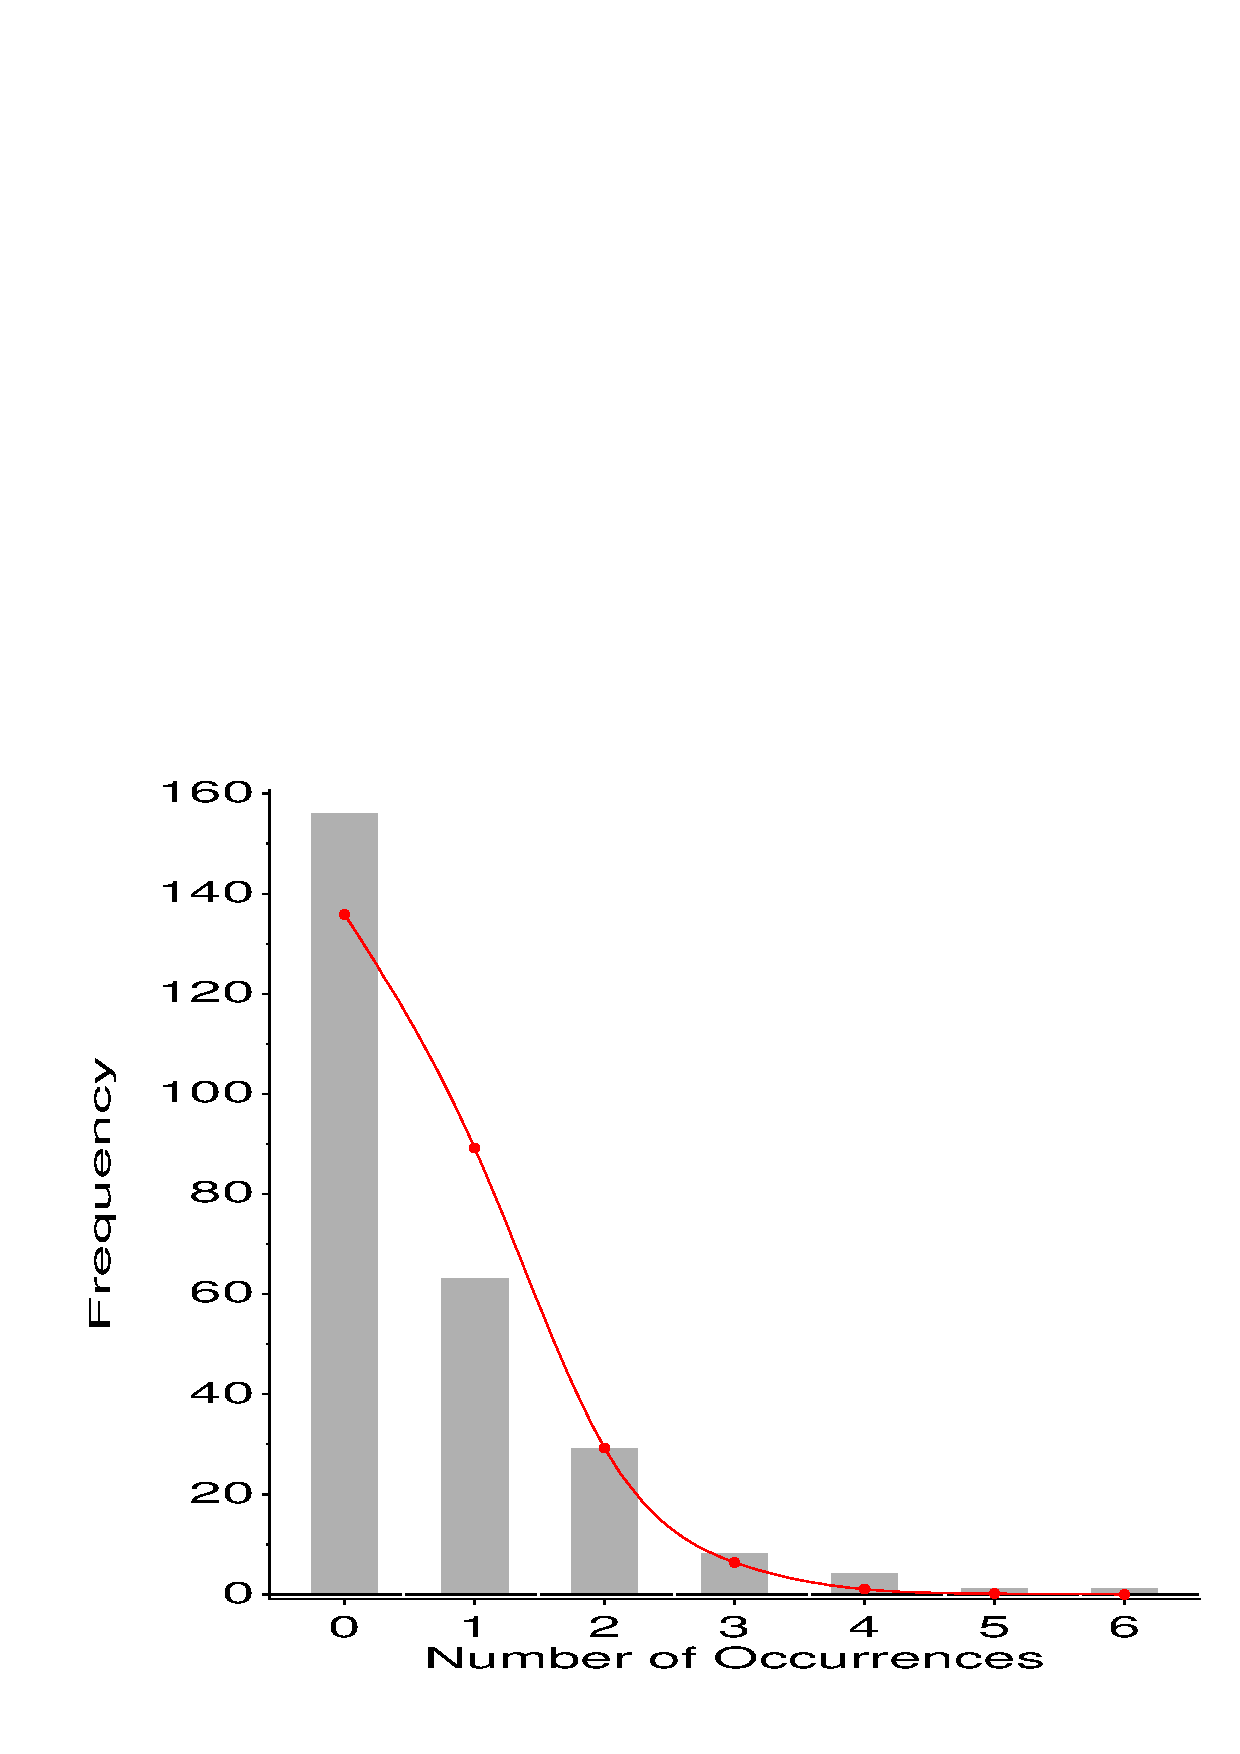
\includegraphics[width=1\linewidth]{fig/madfit1}
 \end{minipage}%
 \hfill
 \begin{minipage}[c]{.49\dispwidth}
 Problems:
	\begin{itemize*}
	\item largest frequencies dominate display
	\item must assess deviations vs. a curve
	\end{itemize*}
 \end{minipage}
	
\end{frame}

\begin{frame}[fragile]
  \frametitle{Hang \& root them $\rightarrow$ Hanging rootograms}
  \citet{Tukey:72,Tukey:77}:
  \begin{itemize*}
  \item shift histogram bars to 
  the fitted curve $\rightarrow$ judge deviations vs. horizontal line.
  \item plot $\sqrt{\mbox{freq}} \rightarrow$
  smaller frequencies are emphasized.
  \end{itemize*}

  \begin{Code}
   %goodfit(data=madison, var=count, freq=blocks, 
     dist=poisson, \sasemph{out=fit});
   \sasemph{%rootgram(data=fit, var=count, obs=blocks);}
  \end{Code}
    \begin{center}
	\includegraphics[width=.45\dispwidth,clip]{fig/madfit3}
    \end{center}

\end{frame}

\begin{frame}[fragile]
  \frametitle{Highlight differences $\rightarrow$ Deviation rootograms}
  \begin{itemize*}
  \item Emphasize differences between observed and fitted frequencies
  \item Draw bars to show the gaps (\texttt{btype=dev})
  \end{itemize*}

  \begin{Code}
   %goodfit(data=madison, var=count, freq=blocks, 
     dist=poisson, out=fit);
   %rootgram(data=fit, var=count, obs=blocks, \sasemph{btype=dev});
  \end{Code}
    \begin{center}
	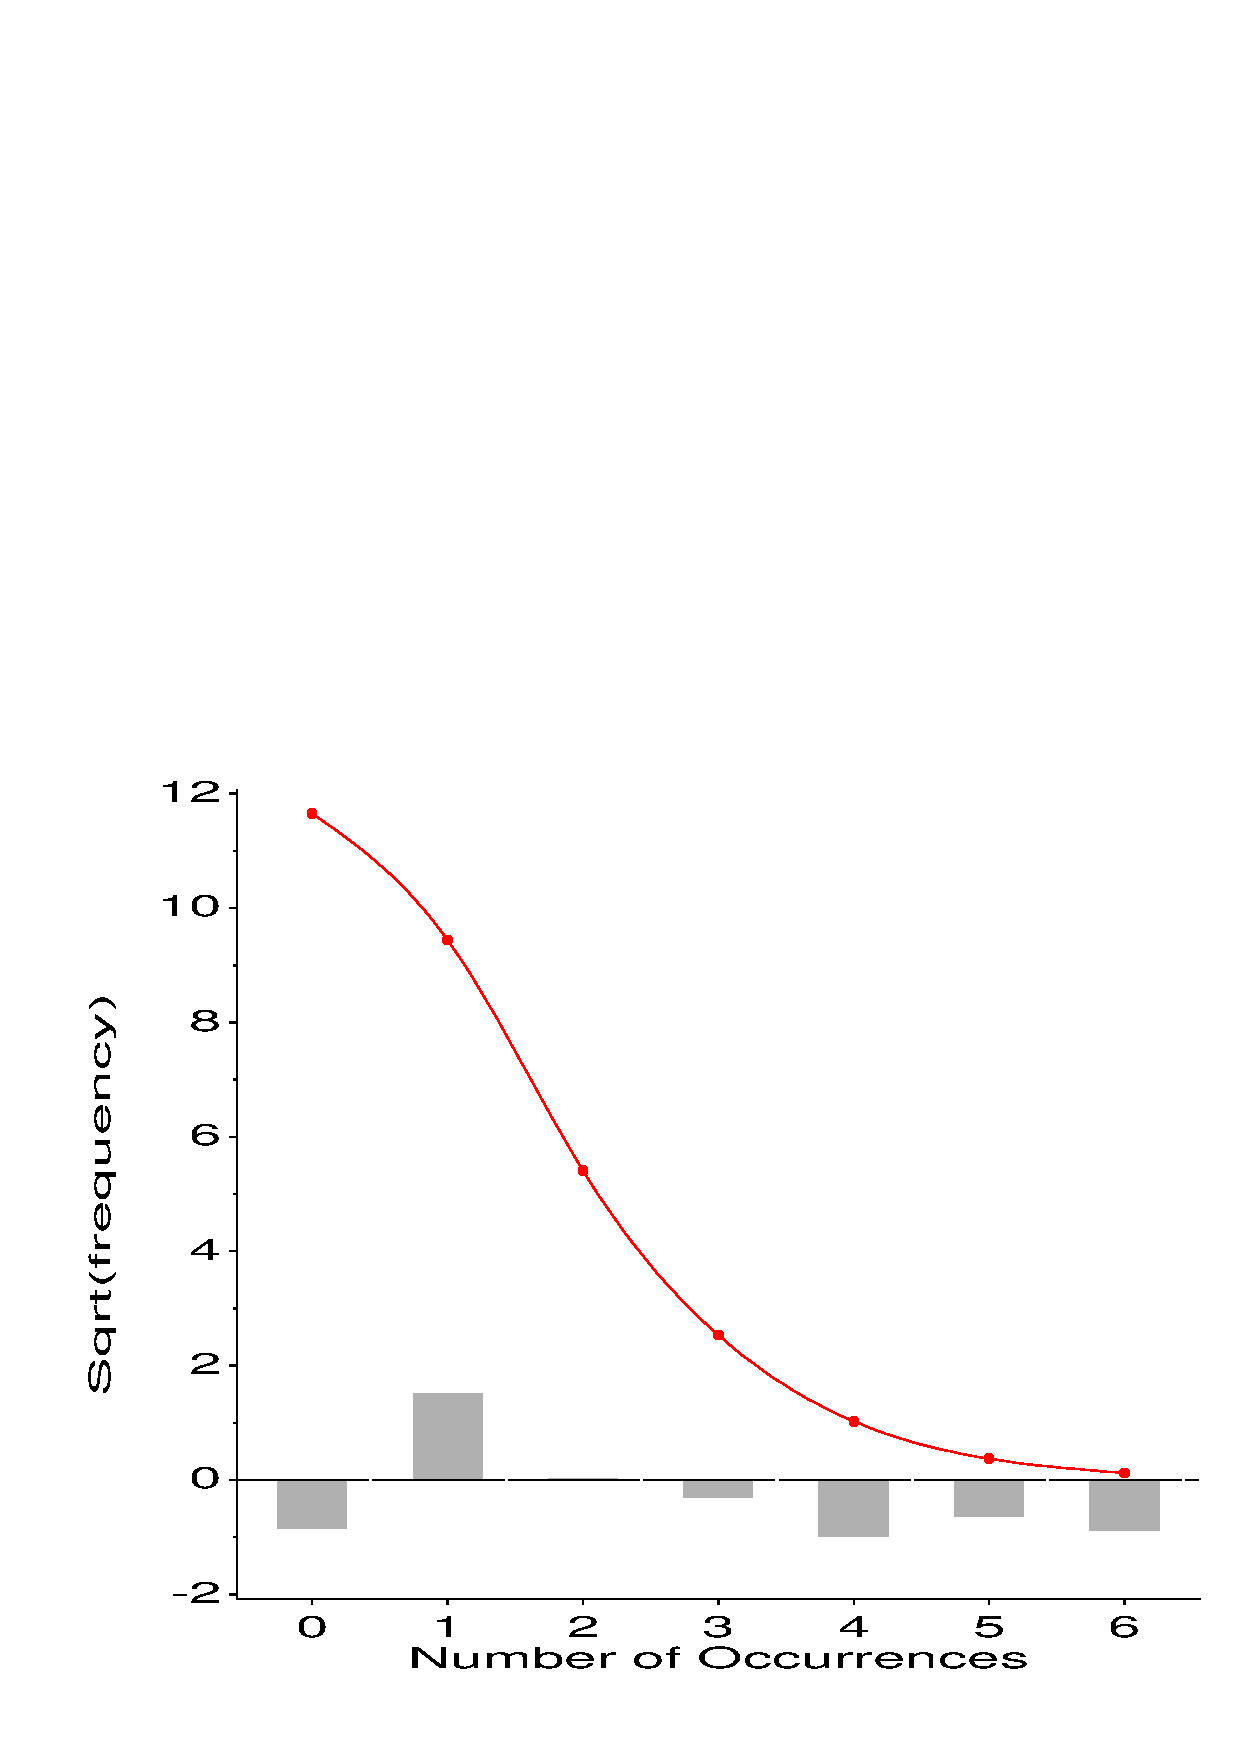
\includegraphics[width=.45\dispwidth,clip]{fig/madfit4}
    \end{center}

\end{frame}

\subsection{Ord plots: diagnose form}
\begin{frame}

\frametitle{Ord plots: Diagnose form of discrete distribution}
\begin{itemize}
\item How to tell which discrete distributions are likely candidates?
\item \citet{Ord:67}: for each of Poisson, Binomial, Negative Binomial, and Logarithmic Series distributions,
	\begin{itemize*}
	\item plot of $k p_k / p_{k-1}$ against $k$ is linear
	\item signs of intercept and slope $\rightarrow$ determine the form,
	give rough estimates of parameters
	\end{itemize*}

\begin{center}
%\vspace{1ex}
\renewcommand{\arraystretch}{.85}
\begin{tabular}{|ccll|}\hline
Slope & Intercept & Distribution & Parameter \\
(b)   & (a)       & (parameter)  &  estimate \\ \hline
0     &  $+$      &  Poisson (\(\lambda\)) & \(\lambda = a\)    \\
$-$   &  $+$      &  Binomial (n, p)       & \(p = b / (b-1)\)  \\
$+$   &  $+$      &  Neg. binomial (n,p)      & \(p = 1 - b\)      \\
$+$   &  $-$      &  Log.\ series (\(\theta\)) & \(\theta =  b\) \\
      &      &                     &   \(\theta = - a\) \\ \hline
\end{tabular}
\end{center}

\item Fit line by WLS, using $\sqrt{n_k-1}$ as weights
\end{itemize}
\end{frame}

\begin{frame}[fragile]
\frametitle{Ord plots}
\begin{itemize}
\item \macro{ORDPLOT}
\begin{Code}
 %ordplot(data=madison, count=Count, freq=blocks);
\end{Code}
\end{itemize}

 \begin{minipage}[c]{.4\dispwidth}
	\begin{itemize*}
	\item Diagnoses distribution as NegBin
	\item Estimates $\hat{p} = 0.576$
	\end{itemize*}
 \end{minipage}
 \hfill
 \begin{minipage}[c]{.59\dispwidth}
  \begin{center}
  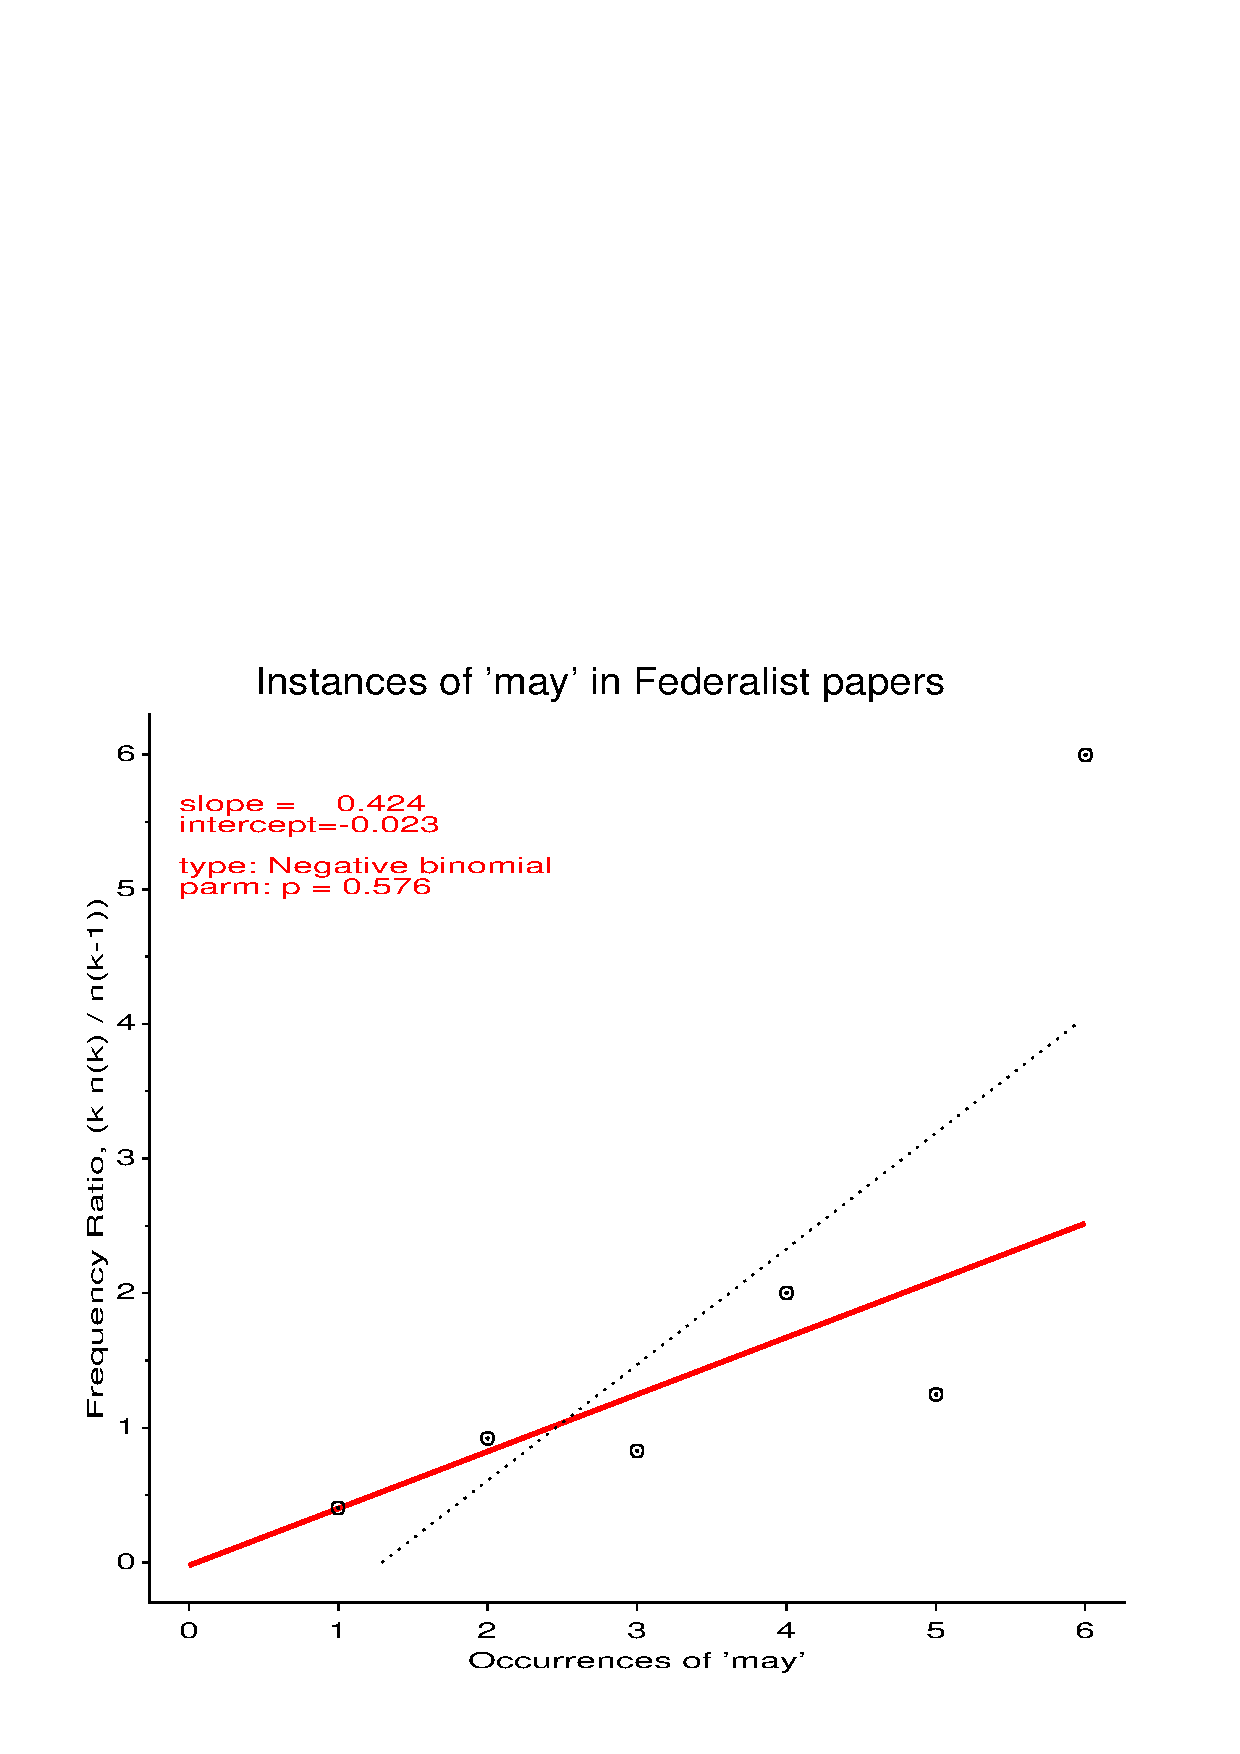
\includegraphics[trim=0 0 0 30,width=\linewidth,clip]{fig/orddemo2}
  \end{center}
 \end{minipage}
\end{frame}
	

\begin{frame}
\frametitle{Ord plots: Other distributions}

 \begin{minipage}[c]{.49\dispwidth}
  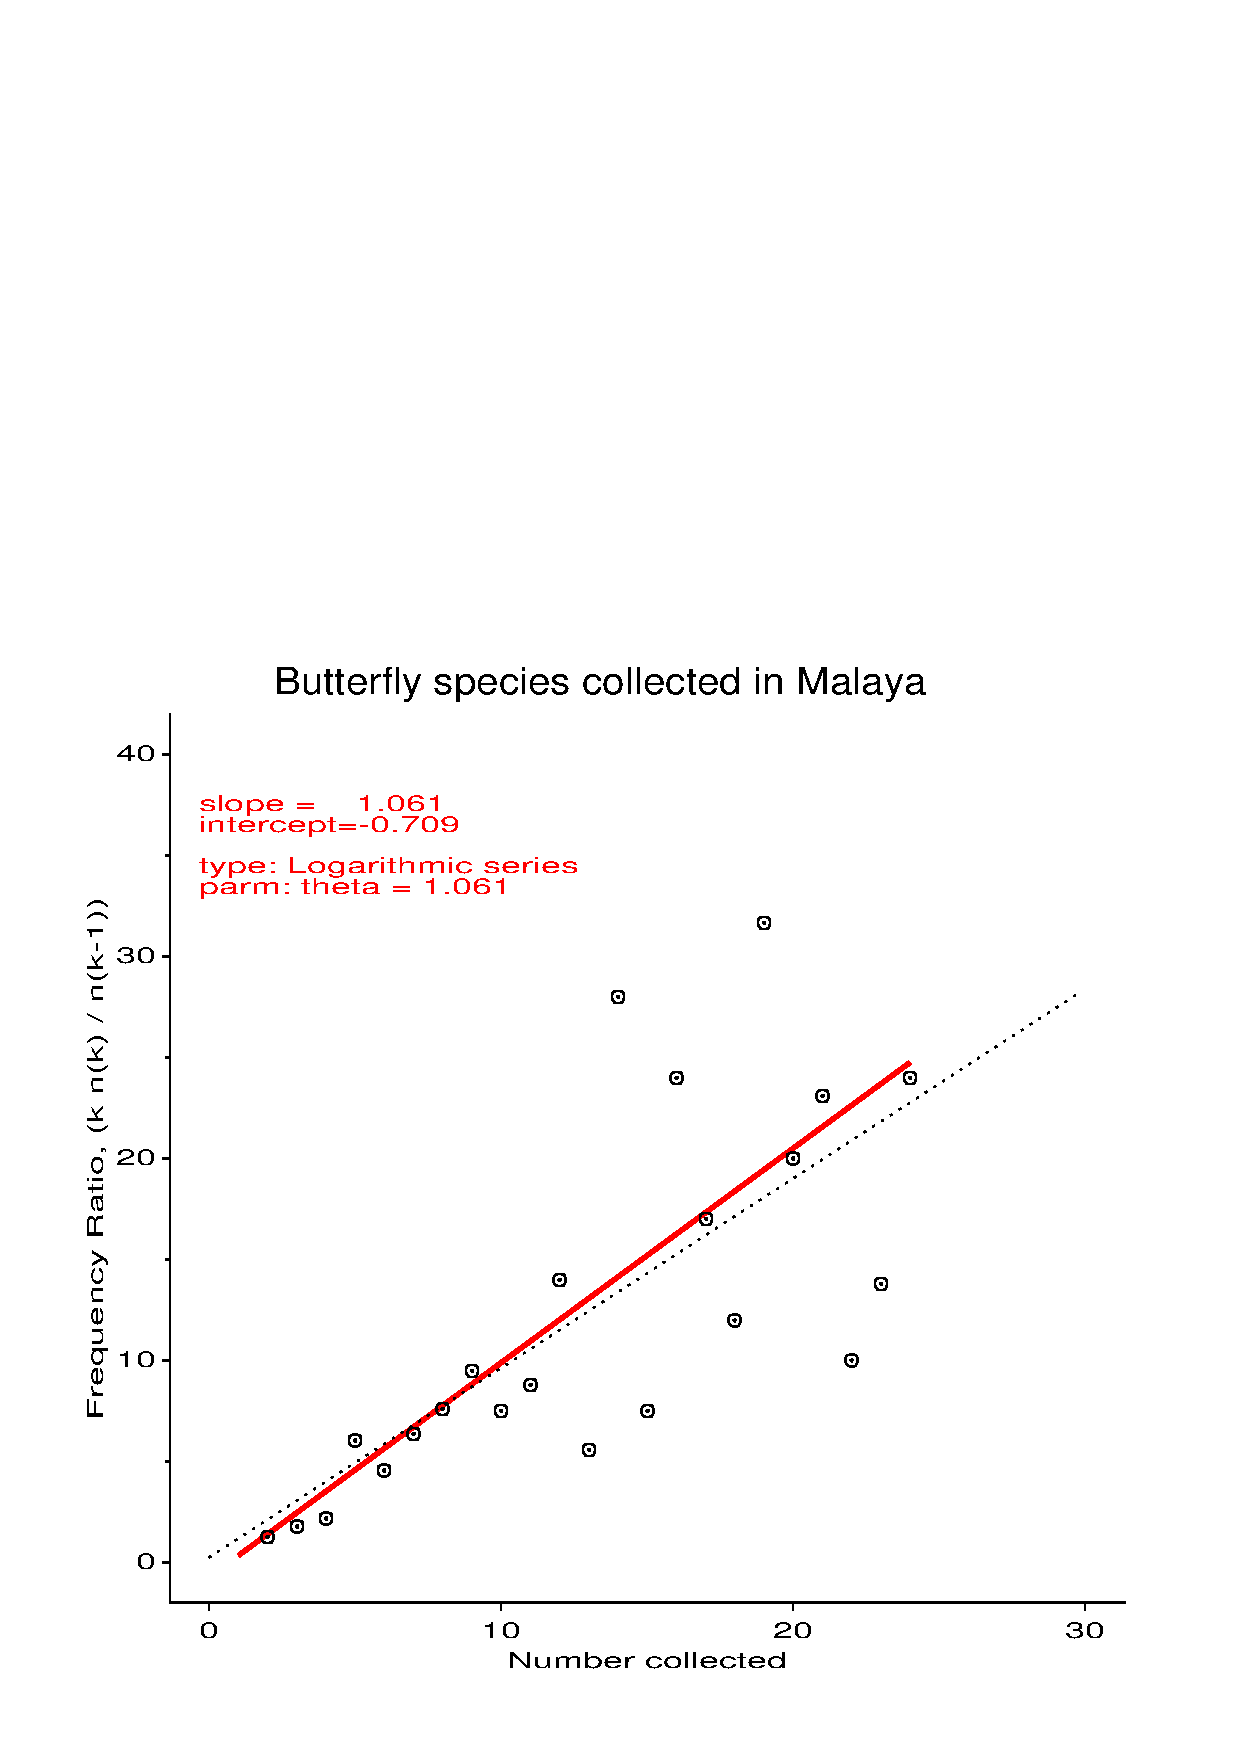
\includegraphics[trim=0 0 0 0,width=\linewidth,clip]{fig/orddemo3}
  \\ \centering Logarithmic series
 \end{minipage}%
 \hfill
 \begin{minipage}[c]{.49\dispwidth}
%  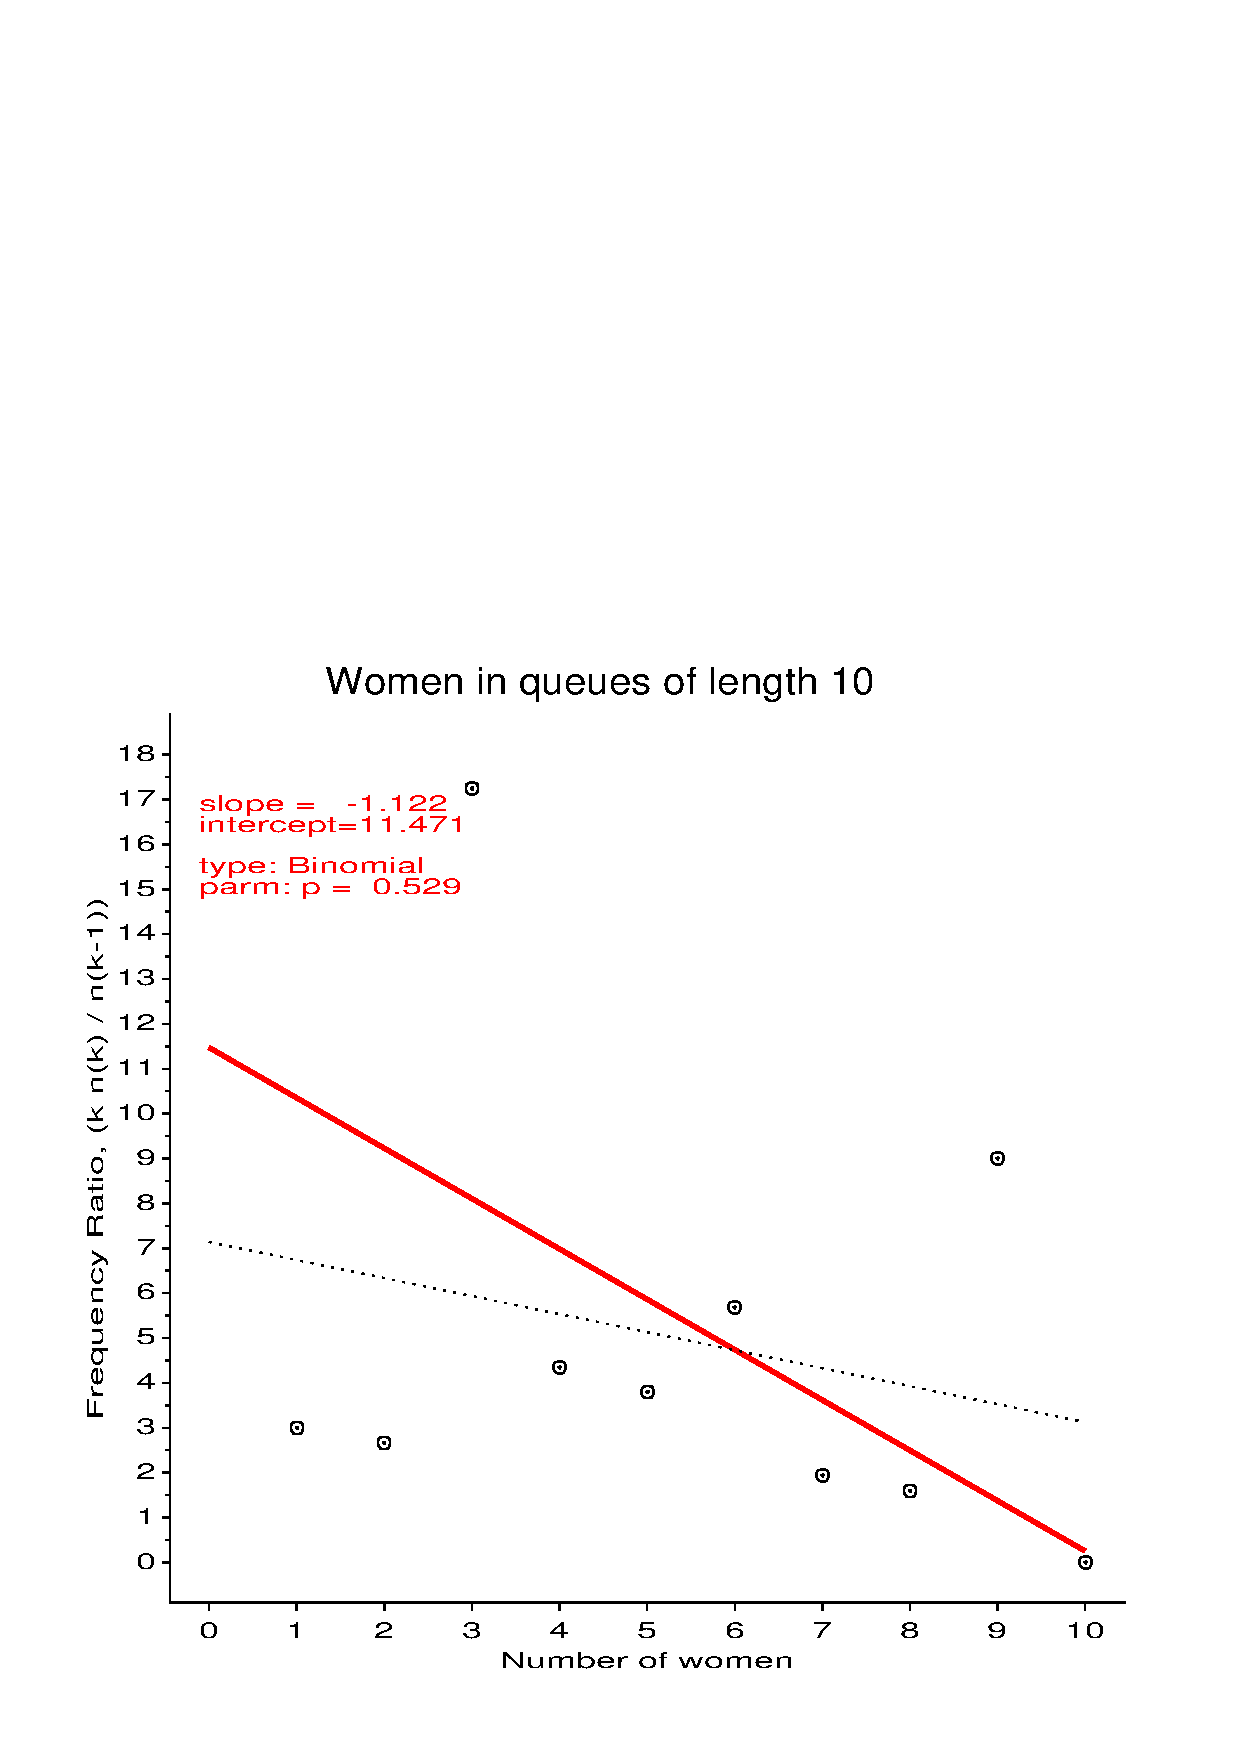
\includegraphics[trim=0 0 0 0,width=\linewidth,clip]{fig/orddemo4}
  \includegraphics[trim=0 0 0 0,width=\linewidth,clip]{fig/saxony4}
  \\ \centering Binomial
 \end{minipage}
\end{frame}

\subsection{Robust distribution plots}
\begin{frame}
  \frametitle{Robust distribution plots: Poisson}
  \begin{itemize}
	\item Ord plots lack robustness 
	\begin{itemize*}
	\item one discrepant freqency, $n_k$
	affects points for both $k$ and $k+1$
	\end{itemize*}

	\item Robust plots for Poisson distribution \citep{HoaglinTukey:85}
	\begin{itemize*}
	  \item For Poisson, plot \boldital{count metameter} =
	  \(\phi \,  ( n_k )  = \log_e ( k ! \,  n_k  /  N )\) vs.\ $k$
	  \item Linear relation $\Rightarrow$ Poisson, slope gives $\hat{\lambda}$
	  \item CI for points, diagnostic (influence) plot
	  \item \macro{POISPLOT}
	\end{itemize*}
  \end{itemize}
\end{frame}

\begin{frame}
  \frametitle{Poissonness plots: Details}
  \begin{itemize}
	\item If the distribution of $n_k$ is Poisson($\lambda$) for some fixed $\lambda$, then each
	observed frequency, $n_k \approx m_k = N p_k$.
	\item Then, setting
\(n_k = N p_k  = { e^{ - \lambda } \:  \lambda^k } /  { k ! }\),
and taking logs of both sides gives
  \[
  \log ( n_k ) = \log \,  N - \lambda  +  k \,  \log \,  \lambda  -
  \log \,  k !
  \]
which can be rearranged to
  \begin{equation*}
  \phi \,  ( n_k )  \equiv \log \left(  \frac{ k ! \:  n_k } {N} \right)
 = - \lambda  +  ( \log \,  \lambda ) \,  k
  \end{equation*}

	\item $\Rightarrow$ if the distribution is Poisson,
	plotting \(\phi ( n_k )\) vs.\ \(k\) should give a line with
	  \begin{itemize*}
	  \item intercept = \(- \lambda\)
	  \item slope = \(\log  \,  \lambda\)
	  \end{itemize*}
	\item Nonlinear relation $\rightarrow$ distribution is \emph{not} Poisson
    \item \citet{HoaglinTukey:85} give details on calculation of confidence intervals
	and influence measures.
  \end{itemize}
\end{frame}

\begin{frame}[fragile]
  \frametitle{\macrot{POISPLOT}: example}
  \begin{Input}[fontsize=\small]
title "Instances of 'may' in Federalist papers";
data madison;
   input count blocks;
   label count='Number of Occurrences'
         blocks='Blocks of Text';
datalines;
  0    156
  1     63
  2     29
  3      8
  4      4
  5      1
  6      1
;
\sasemph{%poisplot(data=madison,count=count, freq=blocks)};
  \end{Input}
\end{frame}

\begin{frame}
  \frametitle{\macrot{POISPLOT}: output}
Curvilinear relation $\rightarrow$ distribution is \emph{not} Poisson
 \begin{minipage}[c]{.49\dispwidth}
  \includegraphics[width=1\linewidth]{fig/poisdemo-mad}
  \\ \centering Poissonness plot
 \end{minipage}%
 \hfill
 \begin{minipage}[c]{.49\dispwidth}
  \includegraphics[width=1\linewidth]{fig/poisdemo-mad3}
  \\ \centering Influence plot for change in $\lambda$
 \end{minipage}

\end{frame}

\begin{frame}[fragile]
  \frametitle{Generalized robust distribution plots}
  Other distributions: Analogous plots, for suitable count metameter, 
  $\phi \,  ( n_k )$
  vs.\ $k$.
  \begin{itemize*}
  \item Linear relation $\Rightarrow$ correct distribution, slope gives parameter estimates
  \item CI reflect variability of the individual counts, $n_k$
  \item \macro{DISTPLOT}
  \end{itemize*}

  \begin{Code}
  %distplot(data=madison, count=count, freq=blocks,
        \sasemph{dist=negbin});
  \end{Code}

  \begin{center}
	\includegraphics[width=.5\dispwidth,clip]{fig/maddist}
  \end{center}
\end{frame}

\subsection{Using R}
\renewcommand{\FileName}{discreteR}

\begin{frame}[fragile]
  \frametitle{Discrete distributions with R and the vcd package}
In R, discrete distributions are conveniently represented as one-way frequency tables,
\begin{Rin}[baselinestretch=0.8]
> library(vcd)
> data(Federalist)
> Federalist
\end{Rin}
\begin{Rout}
nMay
  0   1   2   3   4   5   6 
156  63  29   8   4   1   1 
\end{Rout}
The goodfit() function in vcd fits a variety of discrete distributions:
\begin{Rin}[baselinestretch=0.8]
> # fit the poisson model
> gf1 <- goodfit(Federalist, type="poisson")
> gf1
\end{Rin}
\begin{Rout}[baselinestretch=0.7,fontsize=\footnotesize]
Observed and fitted values for poisson distribution
with parameters estimated by `ML' 

 count observed       fitted
     0      156 135.89138870
     1       63  89.21114067
     2       29  29.28304617
     3        8   6.40799484
     4        4   1.05169381
     5        1   0.13808499
     6        1   0.01510854
\end{Rout}

\end{frame}

\begin{frame}[fragile]
R is object-oriented.  A goodfit object has print(), summary() and plot() methods:
\begin{Rin}
> summary(gf1)
\end{Rin}

\begin{Rout}
         Goodness-of-fit test for poisson distribution

                      X^2 df     P(> X^2)
Likelihood Ratio 25.24312  5 0.0001250511
\end{Rout}

\begin{Rin}
> plot(gf1, main="Federalist data: Poisson fit")
> plot(gf1, main="Federalist data: Poisson fit", type="dev")
\end{Rin}
% two figures
 \begin{minipage}[b]{.5\linewidth}
  \centering
  \includegraphics[width=.95\linewidth]{fig/federalist1}
 \end{minipage}%
 \begin{minipage}[b]{.5\linewidth}
  \centering
  \includegraphics[width=.95\linewidth]{fig/federalist2}
 \end{minipage}

\end{frame}

\begin{frame}[fragile]
  \frametitle{Discrete distributions with R and the vcd package}

The Poisson distribution 
\begin{Rin}
> # In a poisson, mean = var; this is 'over-dispersed'
>  mean(rep(0:6, times=Federalist))
\end{Rin}
\begin{Rout}
[1] 0.6564885
\end{Rout}
\begin{Rin}
>  var(rep(0:6, times=Federalist))
\end{Rin}
\begin{Rout}
[1] 1.007985
\end{Rout}

The negative binomial distribution, Nbin(r, p) 
allows the data to deviate from a true Poisson according to
a parameter $r>0$.
\begin{Rin}
> ## try negative binomial distribution (r, p)
> gf2 <- goodfit(Federalist, type = "nbinomial")
> summary(gf2)
\end{Rin}

\begin{Rout}
         Goodness-of-fit test for nbinomial distribution

                      X^2 df  P(> X^2)
Likelihood Ratio 1.964028  4 0.7423751
\end{Rout}
This has an acceptable fit to the Federalist data

\end{frame}

\begin{frame}[fragile]
  \frametitle{Discrete distributions with R and the vcd package}

Compare the fits side-by-side:
\begin{Rin}
> plot(gf2, main="Federalist data: Negative binomial fit")
> plot(gf1, main="Federalist data: Poisson fit")
\end{Rin}
% two figures
 \begin{minipage}[b]{.5\linewidth}
  \centering
  \includegraphics[width=.95\linewidth]{fig/federalist3}
 \end{minipage}%
 \begin{minipage}[b]{.5\linewidth}
  \centering
  \includegraphics[width=.95\linewidth]{fig/federalist1}
 \end{minipage}

{\large\bfseries Conclusions:}
\begin{itemize*}
  \item Perhaps marker words like 'may' do not occur with constant probability in all
  blocks of text
  \item Perhaps the blocks of text were written under different circumstances
\end{itemize*}

\begin{comment}
> # geometric = NBin (1,p)
> gf3 <- goodfit(Federalist, type = "nbinomial", par = list(size = 1))
> summary(gf3)

\begin{Rout}
         Goodness-of-fit test for nbinomial distribution

                      X^2 df  P(> X^2)
Likelihood Ratio 2.294143  5 0.8071267
\end{Rout}
> plot(gf3, main="Federalist data: Geometric distribution, NBin(1,p)")
\end{comment}

\end{frame}

\begin{frame}[fragile]
vcd includes Ord\_plot() and distplot() functions. E.g.,
\begin{Rin}
> Ord_plot(Federalist, 
       main = "Instances of 'may' in Federalist papers")
\end{Rin}
  \begin{center}
        \includegraphics[width=.72\dispwidth,clip]{fig/federalist5}
  \end{center}

\end{frame}


\section{Testing association}
\section{Association plots}\label{sec:twoway-assoc}
In the \IX{sieve diagram} the foreground (rectangles) shows expected
frequencies; deviations from independence are shown by color and
density of shading.  The association plot
\citep{Cohen:80,Friendly:91}
puts deviations from independence in the foreground:  the area
of each box is made proportional to observed $-$ expected frequency.
This graphical method is described in more detail in \SSSGref{10.2.1},
which also lists the program used to produce the association plot.

For a two-way contingency table, the signed contribution to Pearson
\(\chi^2\) for cell \(i, \, j\) is
\begin{equation*}
  d_{ij}  =
  \frac{ n_{ij} - m_{ij} } { \sqrt { m_{ij} } }
 = \mbox{ std. residual},
  \qquad
  \chi^2 = \sum_{ij} \:  ( d_{ij} )^2
\end{equation*}

In the \glossterm{association plot}, each cell is shown by a
rectangle:

\begin{itemize*}
\item (signed) height \(\sim d_{ij}\)

\item width = \(\sqrt { m_{ij}}\).
\end{itemize*}
so, the area of each cell is proportional to the raw residual,
\glosstex{residuals}
\(n_{ij} - m_{ij}\).
The rectangles for each row in the table are positioned relative to a
baseline representing independence (\(d_{ij} = 0\)) shown by a dotted
line.  Cells with observed \(>\) expected frequency rise above the line
(and are colored black); cells that contain less than the expected
frequency fall below it (and are shaded gray).

\begin{figure}[htb]
  \centering
  \includegraphics[width=.7\linewidth]{ch3/fig/assocplt.eps}
  \caption{Association plot for hair-color, eye-color.}\label{fig:assocplt}
\end{figure}
\figref{fig:assocplt} shows the association plot for the hair-color,
eye-color data.  Note that the residuals in each row tend to increase
or decrease systematically in each row, except that for hazel eyes.

One virtue of the association plot is that it is quite simple to
interpret.  
\citet{Bertin:81} uses similar graphics to display large complex
\ctabs.  Like the sieve diagram, however, patterns of association
are most apparent when the rows and columns of the display are ordered
in a sensible way.

\section{Summary: Part 1}
\renewcommand{\FileName}{summary1}
% slide template
\begin{frame}
  \frametitle{Summary: Part 1}
  \begin{itemize}
	\item<1->{\large\bfseries Categorical data}
      \begin{itemize*}
	  \item Table form vs.\ case form
	  \item Non-parametric methods vs.\ model-based methods
      \item Response models vs.\ association models
	  \end{itemize*}
	\item<2->{\large\bfseries Graphical methods for categorical data}
      \begin{itemize*}
	  \item Frequency data more naturally displayed as \textbf{count} $\sim$ {area}
	  \item Sieve diagram, fourfold \& mosaic display: compare observed vs.\ expected frequency
	  \item Graphical principles: Visual comparison, effect-ordering, small multiples
	  \end{itemize*}
	\item<3->{\large\bfseries Discrete distributions}
      \begin{itemize*}
	  \item Fit: \texttt{GOODFIT}; Graph: hanging rootograms to show departures 
 	  \item Ord plot: diagnose form of distribution
	  \item \texttt{POISPLOT}, \texttt{DISTPLOT} for robust distribution plots
	  \end{itemize*}
	\item<4->{\large\bfseries Testing association}
     \begin{itemize*}
	  \item Pearson $\chi^2$, L.R. $\chi^2$ (largish samples) vs. Fisher exact test (small samples)
 	  \item CMH tests more powerful for ordinal factors
	  \item Three-way+ tables: Stratified analysis, homogeneity of association
      \item Visualize with Sieve diagram, fourfold \& mosaic display
	  \end{itemize*}
  \end{itemize}
\end{frame}



\endinput


\lecture{Two-way and n-way tables}{Two-way}
%\part{Two-way tables}
\renewcommand{\FileName}{part2}
\part{Two-way tables}
\begin{frame}
  \frametitle{Part 2: Visualizing two-way and \nway\ tables}
 \begin{minipage}[c]{.33\textwidth}
  \includegraphics[width=1\linewidth]{fig/pie2x2g}
  \end{minipage}%
 \hfill
 \begin{minipage}[c]{.33\textwidth}
  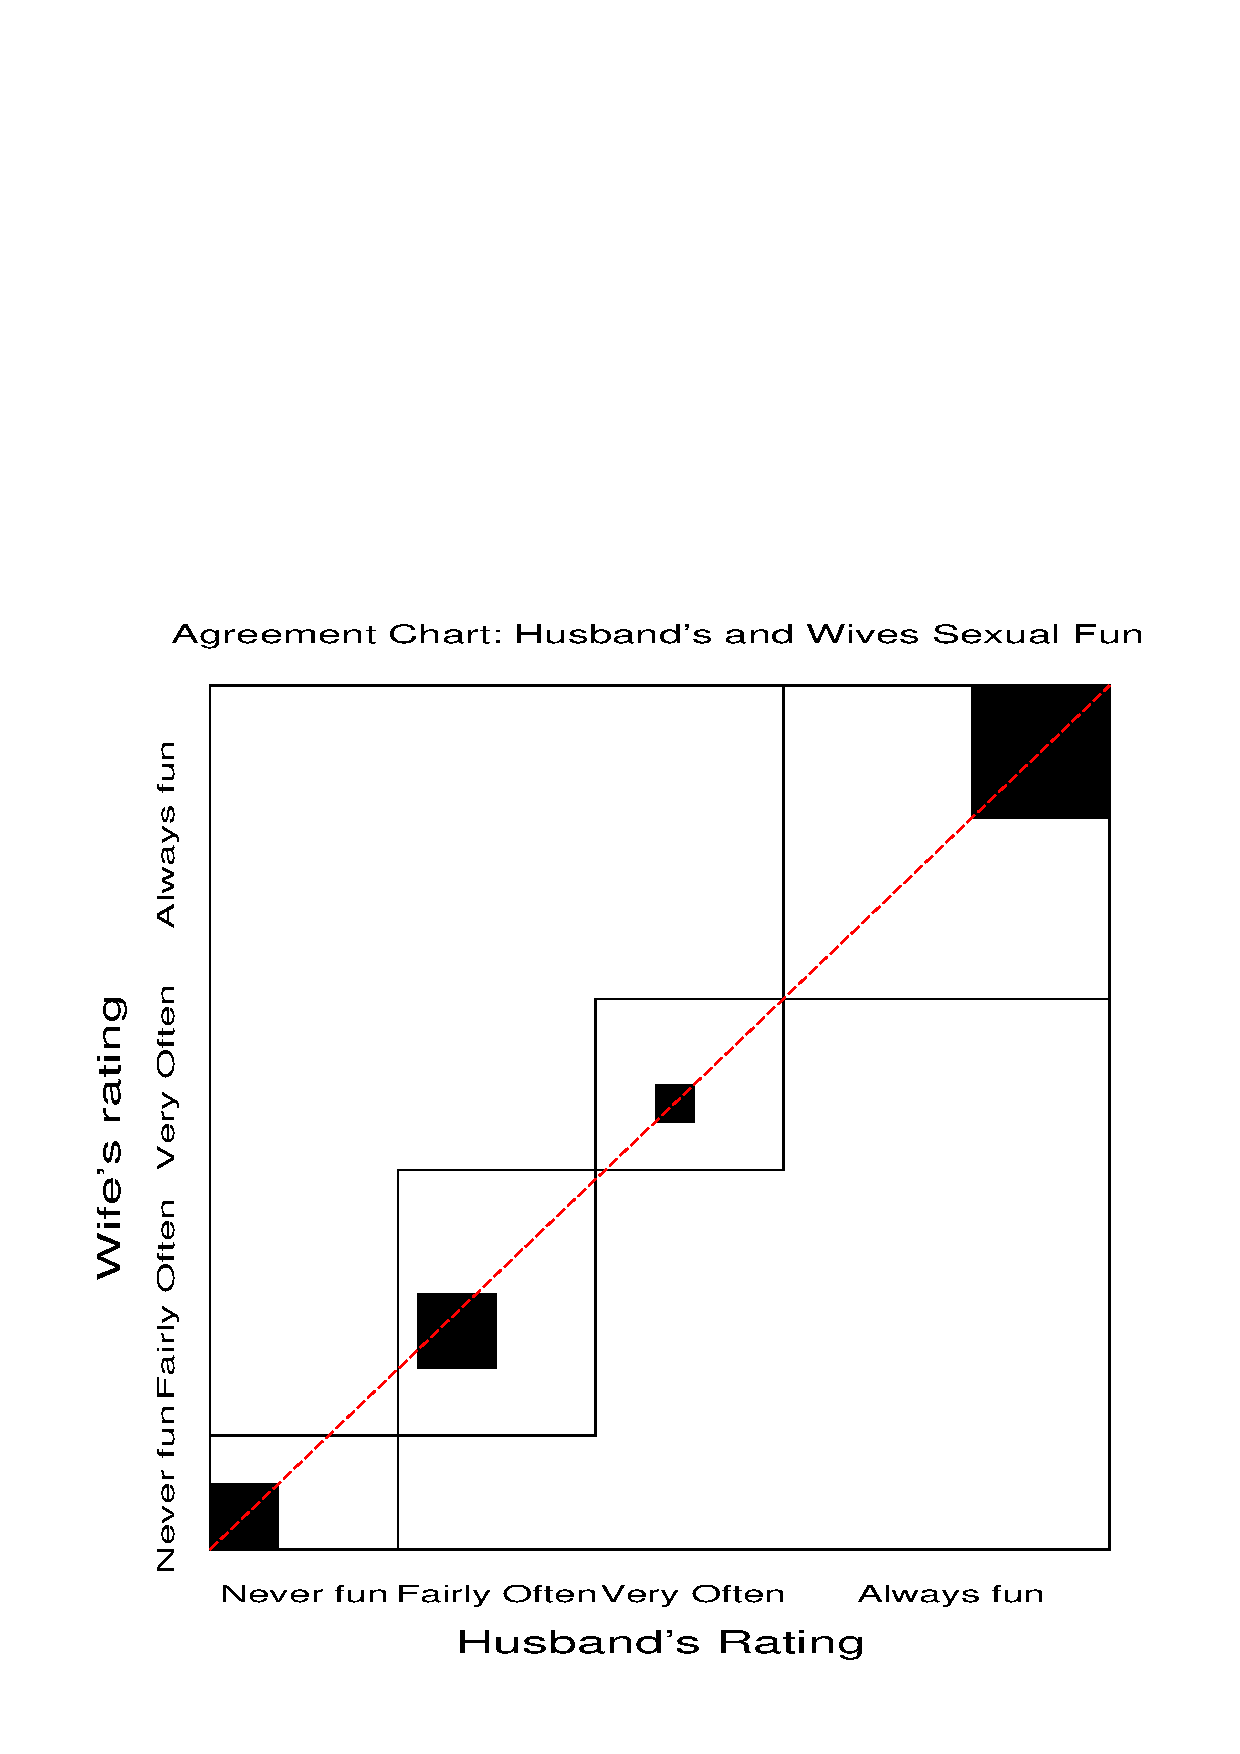
\includegraphics[width=1\linewidth,clip]{fig/agreemt1}
 \end{minipage}
 \hfill
 \begin{minipage}[c]{.33\textwidth}
  \includegraphics[width=1\linewidth,clip]{fig/mosaic3m1}
 \end{minipage}

Topics:
  \begin{itemize*}
    \item $2 \times 2$ tables and fourfold displays
	\item Sieve diagrams
	\item Observer agreement
%	\item Mosaic displays and \loglin\ models for \nway\ tables
	\item Correspondence analysis
  \end{itemize*}
\end{frame}


\renewcommand{\FileName}{vismethods}
\begin{frame}
%\makeatletter\slidebox@restore\makeatother
 
\frametitle{Visualizing contingency tables: software tools}
\begin{itemize}
\item Two-way tables
\begin{itemize*}
\item $2 \times 2$ ($\times k$) tables --- Visualize odds ratio (\macro{FFOLD})
%\item $2 \times 2 \times k$ tables --- Homogeneity of association
\item $r \times 3$ tables --- Trilinear plots (\macro{TRIPLOT})
\item $r \times c$ tables --- Visualize association (\macro{SIEVEPLOT})
\item $r \times c$ tables --- Visualize association (\macro{MOSAIC})
\item Square $r \times r$ tables --- Visualize agreement (\macro{AGREEPLOT})
\end{itemize*}
 
\item \nway\ tables
\begin{itemize*}
\item Fit \loglin\ models, visualize lack-of-fit --- (\macro{MOSAIC})
\item Test \& visualize partial association  --- (\macro{MOSAIC})
\item Visualize pairwise association  --- (\macro{MOSMAT})
\item Visualize conditional association  --- (\macro{MOSMAT})
\item Visualize \loglin\ structure  --- (\macro{MOSMAT})
\end{itemize*}
 
\item Correspondence analysis and MCA --- (\macro{CORRESP})
\item R: most of these in the \pkg{vcd} 
\begin{itemize*}
    \item \func{fourfold}, \func{sieve}, \func{mosaic}, \func{agreementplot}, $\dots$ --- more general
    \item Correspondence analysis: \pkg{ca}
\end{itemize*}

\end{itemize}
\end{frame}
 

\section{2 x 2 tables}
\subsection{2 by 2 tables}\label{sec:twoway-twobytwo}

The $2 \times 2$ \ctab{} of applicants to Berkeley graduate programs in \tabref{tab:berk22} may be regarded as an example of a
\glossterm{cross-sectional study}.
The total of $n = 4,526$ applicants in 1973 has been classified by both
gender and admission status.
Here, we would probably consider the total $n$ to be fixed,
and the cell frequencies $n_{ij},  \: i=1,2; j=1,2$
would then represent a single
\glossterm{multinomial sample} for the cross-classification by two
binary variables,
with probabilities cell $p_{ij},  \: i=1,2; j=1,2$
such that
\begin{equation*}
 p_{11} + p_{12} + p_{21} + p_{22} = 1
 \period
\end{equation*}
The basic null hypothesis of interest for a multinomial sample is that
of independence.  Are admission and gender independent of each other?

Alternatively, if we consider admission the response variable, and
gender an explanatory variable, we would treat the numbers of male
and female applicants as fixed
and consider the cell frequencies to represent two independent
\glossterm{binomial samples} for a binary response.
In this case, the null hypothesis is described as that of homogeneity
of the response proportions across the levels of the explanatory variable.

\subsubsection{Odds and odds ratios}\label{sec:twoway-odds}
\ixon{odds ratio}
Measures of association are used to quantify the strength of association
between variables.  Among the many measures of association for
\ctabs, the \glossterm{odds ratio} is particularly useful for
$2 \times 2$ tables, and is a fundamental parameter in several
graphical displays and models described later.
Other measures of strength of association for $2 \times 2$ tables
are described in \CDAref{\C 2} and \citet[{}\S 2.2]{Agresti:96}.

For a binary response, where the probability of a ``success'' is $\pi$,
the \emph{odds} of a success is defined as
\begin{equation*}
 \textrm{odds} = \frac{\pi}{1-\pi} \period
\end{equation*}
Hence, $\textrm{odds} = 1$ corresponds to $\pi = 0.5$, or success and
failure equally likely.   When success is more likely than failure
$\pi > 0.5$, and the $\textrm{odds} > 1$;  for instance, when $\pi = 0.75$,
$\textrm{odds} = .75/.25 =3$, so a success is three times as likely
as a failure.  When failure is more likely, $\pi < 0.5$, and the $\textrm{odds} < 1$;  for instance, when $\pi = 0.25$,
$\textrm{odds} = .25/.75 =\frac{1}{3}$.

The odds of success thus vary multiplicatively around 1.  Taking logarithms
gives an equivalent measure which varies additively around 0, called the
\emph{log odds} or \emph{logit}
\begin{equation*}
 \logit (\pi) \equiv \log (\mbox{odds}) = \log \left( \frac{\pi}{1-\pi} \right)
 \period
\end{equation*}
The logit is symmetric about $\pi = 0.5$, in that
$\logit (\pi) = - \logit (1-\pi)$.

A binary response for two groups gives a $2 \times 2$ table, with
Group as the row variable, say.  Let $\pi_1$ and $\pi_2$ be the
success probabilities for Group 1 and Group 2.  The \emph{odds ratio}
is just the ratio of the odds for the two groups:
\begin{equation*}%\label{eq:oddsratio}
 \mbox{odds ratio} \equiv \theta =
 \frac{\mbox{odds}_1} {\mbox{odds}_2} =
 \frac{\pi_1 / (1-\pi_1)} {\pi_2 / (1-\pi_2)}
 \period
\end{equation*}

Like the odds itself, the odds ratio is always non-negative, between
0 and $\infty$.  When $\theta = 1$, the distributions of success and
failure are the same for both groups (so $\pi_1 = \pi_2$);  there is
no association between row and column variables, or the response
is independent of group.
When $\theta > 1$, Group 1 has a greater success probability;
when $\theta < 1$, Group 2 has a greater success probability.

Similarly, the odds ratio may be transformed to a log scale, to give
a measure which is symmetric about 0.
The \emph{log odds ratio}, symbolized by $\psi$, is just the difference
between the logits for Groups 1 and 2:
\begin{equation*}%\label{eq:logoddsratio}
 \mbox{log odds ratio} \equiv \psi
 = \log (\theta)
 = \log \left[ \frac{\pi_1 / (1-\pi_1)} {\pi_2 / (1-\pi_2)} \right]
 = \logit (\pi_1) - \logit(\pi_2)
 \period
\end{equation*}
Independence corresponds to $\psi =0$, and reversing the rows or columns
of the table merely changes the sign of $\psi$.

For sample data, the \emph{sample odds ratio} is the ratio of the sample
odds for the two groups:
\begin{equation}\label{eq:soddsratio}
 \hat{\theta} =  \frac{p_1 / (1-p_1)} {p_2 / (1-p_2)} =
 \frac{ n_{11} / n_{12} }{ n_{21} / n_{22}} =
 \frac{ n_{11} n_{22} } {n_{12} n_{21}}
 \period
\end{equation}

We described the odds ratio for a sampling context of independent binomial
samples, but actually, the odds ratio is an appropriate measure of strength
of association for all the standard sampling schemes, because it treats
the variables symmetrically.  It does not matter whether the row or column
variable is the response, or whether both variables are treated as
responses.  Other measures of strength of association, not described here,
\emph{do} distinguish between explanatory and response variables.

The sample estimate $\hat{\theta}$ in \eqref{eq:soddsratio} is the
maximum likelihood estimator of the true $\theta$.
The sampling distribution of $\hat{\theta}$ is asymptotically normal
as $n \rightarrow \infty$, but may be highly skewed in small to
moderate samples.  Consequently, inference for the odds ratio
is more conveniently carried out in terms of the log odds ratio,
whose sampling distribution is more closely normal, with mean
$\psi = \log (\theta)$, and asymptotic standard error (ASE)
\begin{equation}\label{eq:aselogtheta}
 \mbox{ASE }_{\log (\theta)} \equiv \hat{s} (\hat{\psi} ) =
 {\left\{
 \frac{1}{n_{11}} + \frac{1}{n_{12}} + \frac{1}{n_{21}} + \frac{1}{n_{22}}
 \right \} }^{1/2}
 =   {\left\{ \sum \sum n_{ij}^{-1} \right \} }^{1/2}
\end{equation}
A large-sample $100(1-\alpha)$\% confidence interval for $\log (\theta)$ may therefore
be calculated as $\log (\theta) \pm z_{1-\alpha/2} \, \mbox{ASE }_{\log (\theta)}$,
where $z_{ 1 - \alpha  / 2 }$ is the cumulative normal quantile with
$1-\alpha/2$ in the lower tail.
Confidence intervals for $\theta$ itself are obtained by exponentiating
the end points of the interval for $\log (\theta)$.

However, $\hat{\theta}$ is 0 or $\infty$ if any $n_{ij}=0$.
\citet{Haldane:55} and \citet{GartZweiful:67} showed that improved
estimators of $\theta$ and $\psi = \log (\theta)$ are obtained by
replacing each $n_{ij}$ by $[n_{ij} + \frac{1}{2}]$ in \eqref{eq:soddsratio}
and \eqref{eq:aselogtheta}.
This adjustment is preferred in small samples, and required if any
zero cells occur.  In large samples, the effect of adding 0.5 to each
cell becomes negligible.


\begin{Example}[berkeley1a]{Berkeley admissions}
Odds ratios and many other measures of association not described here
are produced with \PROC{FREQ} when you specify the \opt{MEASURES}{FREQ}
in the \stmt{TABLES}{FREQ}.
For the Berkeley admissions data, the frequency table in \outref{out:berkfreq.1} and the various measures of association
are produced by these statements:
%% input: /Users/friendly/sasuser/catdata/berkfreq.sas
%% last modified: 14-Jul-99  9:36
\begin{listing}
%include catdata(berkeley);

proc freq data=berkeley order=data;
   weight freq;
   tables gender*admit / nocol measures;
   format admit admit. gender $sex.;
\end{listing}

\begin{Output}[htb]
\caption{Admission to Berkeley graduate programs: Odds ratio and relative risk}\label{out:berkfreq.2}
\small
\verbatiminput{ch\thechapter/out/berkfreq.2}
\end{Output}
The odds ratio is displayed in a section of the output labeled
``Estimates of the Relative Risk'', as the value associated
with a Case-Control study.  This portion of the output is shown in
\outref{out:berkfreq.2}.
The value $\hat{\theta} = 1.84 = (1198 \times 1278) / (557 \times 1493)$ indicates that males are nearly
twice as likely to be admitted as females.
We describe a visualization method for odds ratios in $2 \times 2$
tables in \secref{sec:twoway-fourfold}
and return to the Berkeley data in \exref{ex:berkeley2}.
See \CDAref{\S 2.4--2.5} for discussion of relative risk and other
measures of association in $2 \times 2$ tables.
\end{Example}
\ixoff{odds ratio}
\section{Two-way tables}
\renewcommand{\FileName}{twoway}
% slide template
\begin{frame}
  \frametitle{Two-way frequency tables}
\input{tab/hair-eye}

\begin{itemize}
 \item With a $\chi^2$ test (\PROC{FREQ}) we can tell that hair-color and eye-color are associated.
 \item The more important problem is to understand \alert{how} they are associated.
 \item Some graphical methods:
	\begin{itemize*}
		\item Sieve diagrams
		\item Agreement charts (for square tables)
		\item Mosaic displays
	\end{itemize*}
\end{itemize}
\end{frame}

\subsection{Sieve diagrams}
\begin{frame}
  \frametitle{Two-way frequency tables: Sieve diagrams}
  \begin{itemize}
	\item{\large\bfseries count $\sim$ area}
      \begin{itemize*}
	  \item When row/col variables are independent, $n_{ij} \approx \hat{m}_{ij} \sim n_{i+}
	  n_{+j}$
	  \item $\Rightarrow$ each cell can be represented as a rectangle,
	  with area = height $\times$ width $\sim$ frequency, $n_{ij}$ (under independence)
	  \end{itemize*}
  \end{itemize}
% 	  \begin{center}
% 	  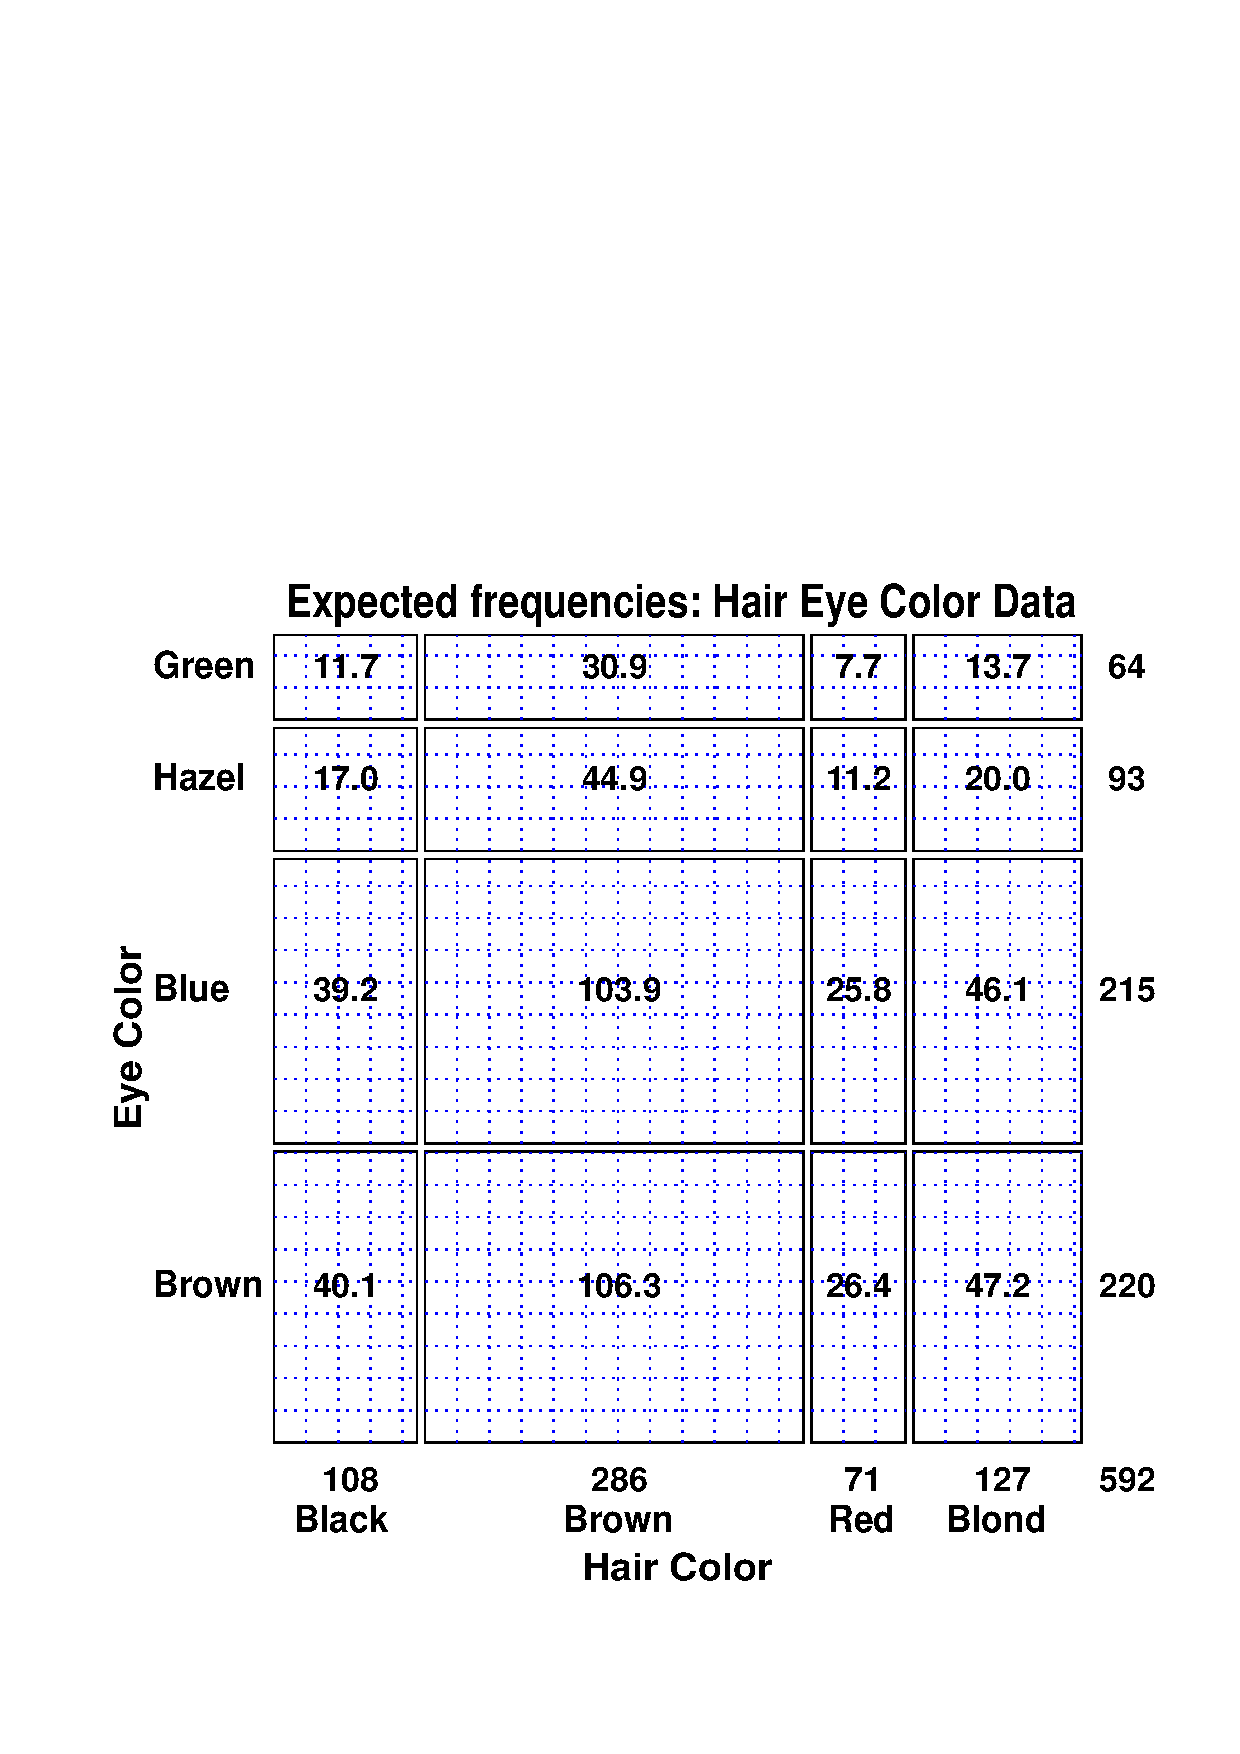
\includegraphics[width=.65\textwidth,clip]{fig/sieve0}
% 	  \end{center}
 \begin{columns}
   \begin{column}{.5\textwidth}
	  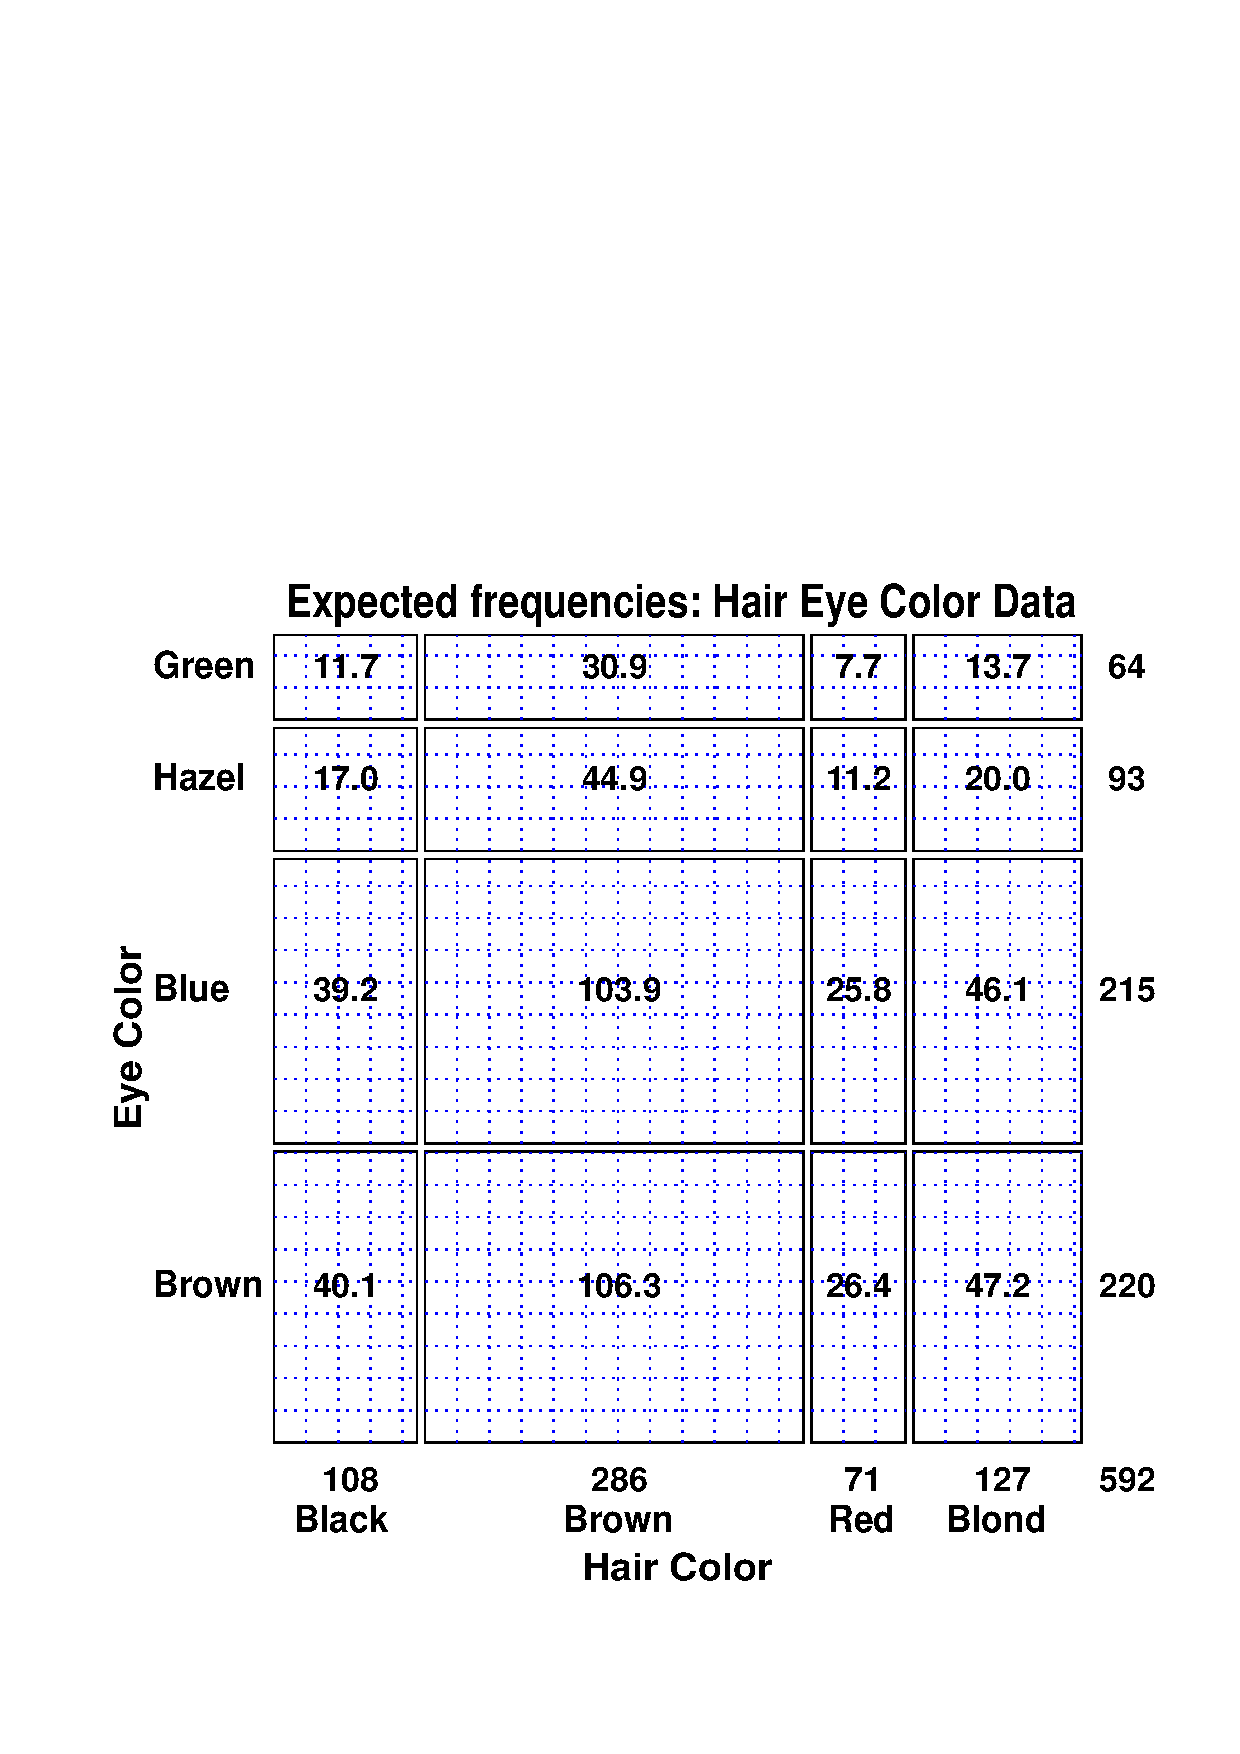
\includegraphics[width=\linewidth,clip]{fig/sieve0}
   \end{column}
   \begin{column}{.5\textwidth}
      \begin{itemize}
       \item This display shows \alert{expected frequencies}, assuming independence, as \# boxes within each cell
       \item The boxes are all of the same size (equal density)
       \item Real sieve diagrams use \# boxes = \alert{observed frequencies}, $n_{ij}$
      \end{itemize}

	
   \end{column}
 \end{columns}

\end{frame}

\begin{frame}
  \frametitle{Sieve diagrams}
  \begin{itemize*}
	\item Height/width $\sim$ marginal frequencies, $n_{i+}$,
	 $ n_{+j}$
	\item Area $\sim$ expected frequency, $\hat{m}_{ij} \sim n_{i+}
	  n_{+j}$
	\item Shading $\sim$ observed frequency, $n_{ij}$, \blue{color}: sign$(n_{ij} -
	\hat{m}_{ij})$.
	\item \boldital{Independence}: Shown when density of shading is uniform.
  \end{itemize*}
	  \vspace{0.5ex}
	  \begin{center}
	  \includegraphics[width=.5\textwidth,clip]{fig/sieve1a1}
	  \end{center}
\end{frame}

\begin{frame}
  \frametitle{Sieve diagrams}
  \begin{itemize*}
	\item {\large\bfseries Effect ordering}: Reorder rows/cols to make the
	pattern coherent
  \end{itemize*}
	  \vspace{1ex}
	  \begin{center}
	  \includegraphics[width=.6\textwidth,clip]{fig/sieve1a2}
	  \end{center}
\end{frame}

\begin{frame}
  \frametitle{Sieve diagrams}
  \begin{itemize*}
	\item Vision classification data for 7477 women
  \end{itemize*}
	  \vspace{1ex}
	  \begin{center}
	  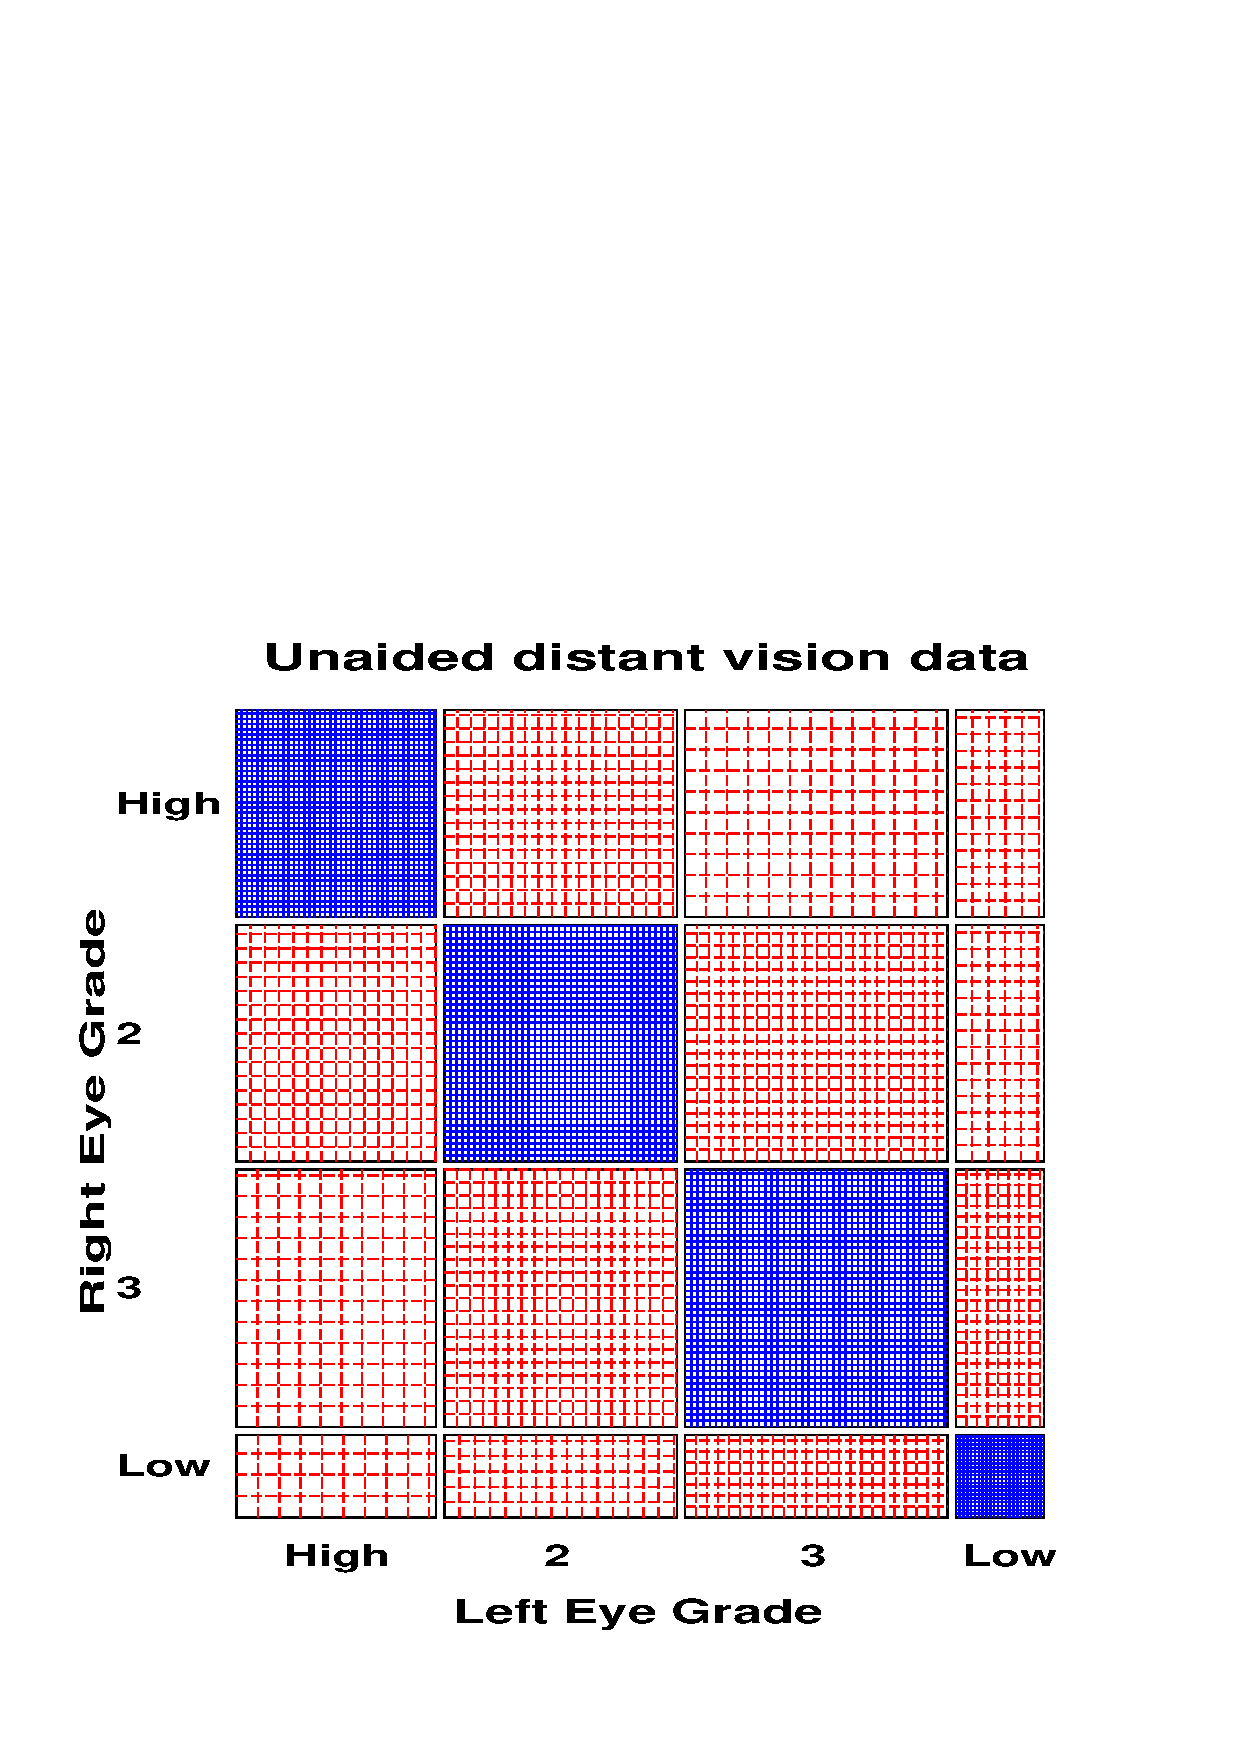
\includegraphics[width=.6\textwidth,clip]{fig/sieve2}
	  \end{center}
\end{frame}

\begin{comment}
\begin{frame}[fragile]
  \frametitle{Sieve diagrams: SAS Example}
\begin{Input}[fontsize=\small,label=\fbox{\texttt{sieve2.sas}},baselinestretch=0.8]
proc iml;
  %include iml(sieve);
    \sascomment{*-- frequency table;}
  tab = \{1520   266   124    66,
          234  1512   432    78,
          117   362  1772   205,
           36    82   179   492 \};
    \sascomment{*-- variable and level names;}
  vnames = \{'Right Eye Grade' 'Left Eye Grade'\};
  lnames = \{ 'High' '2' '3' 'Low',
             'High' '2' '3' 'Low'\};
  title  = \{'Unaided distant vision data'\};
    \sascomment{*-- Global options;}
  \sasemph{run sieve(tab, vnames, lnames, title );}
quit;
\end{Input} 
Online weblet: \url{http://datavis.ca/online/sieve/}
\end{frame}
\end{comment}

\begin{frame}[fragile]
  \frametitle{Sieve diagrams: SAS Example}
\begin{Input}[fontsize=\small,label=\fbox{\texttt{sievem.sas}},baselinestretch=0.8]
data vision;
  do Left='High', '2', '3', 'Low';
  	do Right='High', '2', '3', 'Low';
        input count @@; output;
        end;
    end;
  label left='Left Eye Grade'  right='Right Eye Grade';
datalines;
       1520   266   124    66
        234  1512   432    78
        117   362  1772   205
         36    82   179   492 
;
%sieveplot(data=vision, var=Left Right,
    title=Unaided distant vision data);
\end{Input} 
Online weblet: \url{http://datavis.ca/online/sieve/}
\end{frame}

\begin{frame}[fragile]
  \frametitle{Sieve diagrams: n-way tables in R}
\begin{Rin}
> sieve(UCBAdmissions, sievetype='expected')
\end{Rin}
	  \begin{center}
	  \includegraphics[width=.6\textwidth,clip]{fig/berkeley-sieve1}
	  \end{center}

\end{frame}

\begin{frame}[fragile]
  \frametitle{Sieve diagrams: n-way tables in R}
\begin{Rin}
> sieve(UCBAdmissions, shade=TRUE)
\end{Rin}
	  \begin{center}
	  \includegraphics[width=.6\textwidth,clip]{fig/berkeley-sieve2}
	  \end{center}

\end{frame}

\section{Observer Agreement}
\section{Observer agreement}\label{sec:twoway-agree}
Inter-observer agreement is often used as a method of assessing the
reliability of a subjective classification or assessment procedure.
For example, two (or more) clinical psychologists might classify
patients on a scale with categories: normal, mildly impaired,
severely impaired, or ethologists might classify the behavior
of animals in categories of cooperation, dominance and so forth.

A contingency table is formed where the observations are all the
individuals who have been rated or classified.  The rows of the table
refer to the categories used by one observer, while the columns
refer to the categories used by another observer.
In most cases, the same categories are used by both raters,
so the \ctab{} is square, and the entries in the diagonal cells
are the cases where the raters agree.

\begin{Example}[sexisfun1]{Sex is fun} \tabref{tab:sexisfun}
(\citet[Table 2.10]{Agresti:90}, from \citet{Hout-etal:87})
 summarizes the responses of 91
married couples to a questionnaire item:
\begin{quote}
Sex is fun for me and my partner: (a) Never or occasionally, (b)
fairly often, (c) very often, (d) almost always.
\end{quote}
In each row the diagonal entry is not always the largest, though it
appears that the partners tend to agree more often when either responds
``almost always''.
\begin{table}[htb]
\caption[Ratings of a questionnaire item, ``Sex is fun'', by husbands and wives]{Ratings of a questionnaire item, ``Sex is fun'', by husbands and wives. Source: \citet[Table 2.10]{Agresti:90}, from Hout \etal.}\label{tab:sexisfun}
\begin{center}
 \begin{tabular}{l|rrrr|r}
  \hline
            & \multicolumn{4}{c|}{Wife's Rating} & \\
  Husband's & Never & Fairly & Very & Almost &  \\ 
  Rating & fun & often & Often & always & Total \\ 
  \hline
  Never fun     & 7 & 7 & 2 & 3 & 19 \\ 
  Fairly often  & 2 & 8 & 3 & 7 & 20 \\ 
  Very often    & 1 & 5 & 4 & 9 & 19 \\ 
  Almost always & 2 & 8 & 9 & 14 & 33 \\ 
  \hline
  Total & 12 & 28 & 18 & 33 & 91 \\ 
  \hline
 \end{tabular}
\end{center}
\end{table}

\end{Example}

\begin{Example}[MS1]{Diagnosis of MS patients}
\citet{LandisKoch:77} gave data on the diagnostic classification
of multiple sclerosis (MS) patients by two neurologists,
one from Winnipeg and one from New Orleans, who each classified
patients from Winnipeg and New Orleans into one of four
categories:
\begin{seriate}
\item Certain MS,
\item Probable MS,
\item Possible MS,
\item Doubtful, unlikely, or definitely not MS
\end{seriate}
The data from the 69 patients in the New Orleans sample are shown in
\tabref{tab:msdiag}.
There appears to be highest agreement in the Doubtful category, followed by
the Probable category.
\begin{table}[htb]
\caption{Ratings of 69 patients by two neurologists}\label{tab:msdiag}
\begin{center}
 \begin{tabular}{l|rrrr|r}
  \hline
  New Orleans & \multicolumn{4}{c|}{Winnipeg Neurologist} & \\
  Neurologist & Certain & Probable & Possible & Doubtful & Total \\ 
  \hline
  Certain  MS & 5 & 3 & 0 & 0 & 8 \\ 
  Probable MS & 3 & 11 & 4 & 0 & 18 \\ 
  Possible MS & 2 & 13 & 3 & 4 & 22 \\ 
  Doubtful MS & 1 & 2 & 4 & 14 & 21 \\ 
  \hline
  Total       & 11 & 29 & 11 & 18 & 69 \\ 
  \hline
 \end{tabular}
\end{center}
\end{table}


\end{Example}

\subsection{Measuring agreement}\label{sec:agreemeas}
In assessing the strength of agreement we usually have a more
stringent criterion than in measuring the strength of association,
because
observers ratings can be strongly associated without strong agreement.
For example, one rater could use a more stringent criterion and thus consistently rate subjects one category lower (on an ordinal scale) then another rater.
More generally, measures of agreement must take account of the
marginal frequencies with which two raters use the categories.
If observers tend to use the categories
       with different frequency, this will affect measures of
       agreement.
\ix{marginal homogeneity}

\subsubsection{Intraclass correlation}
\ix{intraclass correlation}
\ix{agreement!intraclass correlation}
An analysis of variance framework leads to the {\bf intraclass correlation}
as a measure of inter-rater reliability, particularly when there are
more than two raters.
This approach is not covered here, but various applications are described
by \citet{ShroutFleiss:79}.

\subsubsection{Cohen's Kappa}
\ix{agreement!Cohen's $\kappa$}
\ix{Cohen's $\kappa$|(}
A commonly used measure of agreement,
Cohen's kappa (\(\kappa\))
\citep{Cohen:60,Cohen:68} compares the observed agreement to agreement expected by chance if the two observer's
ratings were independent.
If $p_{ij}$ is the probability that a randomly selected subject is
rated in category $i$ by the first observer and in category $j$ by
the other, then the observed agreement is the sum of the diagonal
entries,  \(P_o  = \sum_i p_{ii}\).  If the ratings were independent,
this probability of agreement (by chance) would be \(P_c = \sum_i p_{i+} \,  p_{+i}\).
Cohen's $\kappa$ is then the ratio of the difference between actual
agreement and chance agreement, $P_o - P_c$, to the maximum value
this difference could obtain:

\begin{equation}\label{eq:kappa}
  \kappa =  \frac{ P_o - P_c } { 1 - P_c }
  \period
\end{equation}

When agreement is perfect, \(\kappa = 1\);  when agreement is no
better than would be obtained from statistically independent ratings,
$\kappa = 0$.
$\kappa$ could conceivably be negative, but this rarely occurs in practice.
The minimum possible value depends on the marginal totals.

For large samples ($n_{++}$), $\kappa$ has an approximate normal
distribution when $H_0 : \kappa = 0$ is true
and its standard error \citep{Fleiss:73,Fleiss-etal:69} is given by
\begin{equation*}
 \hat{\sigma}(\kappa) =  \frac{ P_c + P_c^2 - \sum_i p_{i+} p_{+i} (p_{i+} + p_{+i}) } { n_{++} (1 - P_c)^2 }
 \period
\end{equation*}
Hence, it is common to conduct a test of $H_0 : \kappa = 0$ by
referring $z = \kappa / \hat{\sigma}(\kappa)$
to a unit normal distribution.
The hypothesis of agreement no better than chance is rarely of much
interest, however.  It is preferable to estimate and report a
confidence interval for $\kappa$.

\subsubsection{Weighted Kappa}
The original (unweighted) \(\kappa\) only counts strict agreement (the same
 category is assigned by both observers).  A weighted version of
       \(\kappa\)
                 \citep{Cohen:68} may be used when one wishes to allow for partial agreement.
       For example, exact agreements might be given full weight,
       one-category difference given weight 1/2.  This typically makes sense
       only when the categories are ordered, as in severity of
       diagnosis.

Weighted \(\kappa\) uses weights, $0 \le w_{ij} \le 1$ for each cell in the
table, with $w_{ii} =1$ for the diagonal cells.
In this case $P_o$ and $P_c$ are defined as weighted sums
\begin{eqnarray*}
P_o  & = & \sum_i \sum_j w_{ij} p_{ij} \\
P_c  & = & \sum_i \sum_j w_{ij} p_{i+} p_{+j}\\
\end{eqnarray*}
and these weighted sums are used in \eqref{eq:kappa}.

For an $r \times r$ table, two commonly-used pattern of weights are those based on
equal spacing of weights
\citep{CicchettiAllison:71}
for a near-match,
%$w_{ij} = 1 - \frac{|i-j|}{r-1}$
and
\emph{Fleiss-Cohen weights}
\citep{FleissCohen:73}, based on an inverse-square
spacing,
% $w_{ij} = 1 - \frac{|i-j|^2}{(r-1)^2}$.
\begin{eqnarray*}
w_{ij} = & 1 - \frac{|i-j|}{r-1} & \quad\quad\mbox{equal spacing} \\
w_{ij} = & 1 - \frac{|i-j|^2}{(r-1)^2} & \quad\quad\mbox{Fleiss-Cohen}
\end{eqnarray*}
\PROC{FREQ} uses the integer (equal) spacing weights by default.
The Fleiss-Cohen weights attach greater importance
to near disagreements, as you can see below for a $4 \times 4$ table.
These weights also provide a measure equivalent to the intraclass
correlation.

\begin{verbatim}
       Integer Spacing                 Fleiss-Cohen Weights
   1     2/3     1/3       0          1     8/9     5/9      0
 2/3       1     2/3     1/3        8/9       1     8/9    5/9
 1/3     2/3       1     2/3        5/9     8/9       1    8/9
   0     1/3     2/3       1          0     5/9     8/9      1
\end{verbatim}

\subsubsection{Computing Kappa with SAS}
In \sasver{6.10} and later, \PROC{FREQ}
provides the $\kappa$ statistic with the \opt{agree}{FREQ}, as shown in
the following example.%
\footnote{In \sasver{7} \PROC{FREQ}
provides 
the \stmt{TEST}{FREQ}
with syntax \pname{TEST KAPPA;} to test the hypothesis that $\kappa = 0$.
You can also request Fleiss-Cohen weights with the option \pname{AGREE (WT=FC)}
in the \stmt{TABLES}{FREQ}.
Standard errors, confidence intervals, and test statistics are large-sample (asymptotic)
by default.  Exact tests are provided by the \stmt{EXACT AGREE}{FREQ}
in \sasver{7}.}

\begin{listing}
title 'Kappa for Agreement';
data fun;
   label husband = 'Husband rating'
         wife    = 'Wife Rating';
   do husband = 1 to 4;
   do wife    = 1 to 4;
      input count @@;
      output;
      end; end;
datalines;
 7     7     2      3
 2     8     3      7
 1     5     4      9
 2     8     9     14
;
proc freq;
   weight count;
   tables husband * wife / noprint agree;
run;
\end{listing}
\ixd{Sex is fun}

This produces the output shown in \outref{out:sexagree}.
Simple kappa gives the unweighted value; you can see there is little
evidence of agreement beyond chance in husbands' and wives' ratings
of their sexual fun.
Weighted kappa uses the equal spacing weights, taking into account
ratings which `nearly' agree.  The weighted sample $\kappa$ is
larger, and the confidence interval does not include 0,
so the weighted agreement is significantly greater than chance,
though again we see that agreement is relatively small.
The test of symmetry (Bowker's test) shown in \outref{out:sexagree}
tests the null hypothesis that non-agreements are symmetric.
\begin{Output}
\caption{Sex is fun data, agreement analysis}\label{out:sexagree}
\small
\verbatiminput{ch3/out/sexagree.out}
\end{Output}
\ix{Cohen's $\kappa$|)}

\subsection[Observer Agreement Chart]{Bangdiwala's Observer Agreement Chart}
\label{sec:twoway:Bangdiwala}
\ix{agreement!observer agreement chart|(}
\ix{observer agreement chart|(}
The observer agreement chart by
\citet{Bangdiwala:87} provides a simple
graphic representation of the strength of agreement in a contingency
table, and a measure of strength of agreement with an intuitive
interpretation.

The agreement chart is constructed as an \(n \times  n\) square,
where $n$ is the total sample size.  Black squares, each of size
\(n_{ii} \times  n_{ii}\), show observed agreement.  These are positioned
within larger rectangles, each of size \(n_{i+} \times  n_{+i}\)
as shown in \figref{fig:agree11}.  The
large rectangle shows the maximum possible agreement, given the
marginal totals.  Thus, a visual impression of the strength of
agreement is given by
\begin{equation}\label{eq:bangb}
  B_N  =
  \frac{ \mbox{area of dark squares}}
  { \mbox{area of rectangles}}  =
  \frac{ \sum_i^k \,  n_{ii}^2 }
  { \sum_i^k \,  n_{i+} \,  n_{+i} }
\end{equation}

\begin{figure}[htb]
  \centering
  \includegraphics[scale=.5]{ch3/fig/agree11}
  \caption[Agreement chart]{Agreement chart for husbands and wives
sexual fun.  The \(B_N\) measure \eqref{eq:bangb} is the ratio of the areas of the
dark squares to their enclosing rectangles, counting only exact
agreement.  \(B_N = 0.146\) for these data.}\label{fig:agree11}

\end{figure}

\subsubsection{Partial agreement}
\ix{agreement!partial}
 Partial agreement is allowed by
including a weighted contribution from off-diagonal cells, $b$
steps from the main diagonal.  For a given cell frequency,
$n_{ij}$, a pattern of weights, $w_1, w_2, \dots,  w_b$ is applied
to the cell frequencies
as shown schematically below:
\begin{equation*}
 \left.
 \begin{array}{ccccc}
   &  & n_{i-b,i} &  & \\
        &  & \vdots    &  & \\
        n_{i, i-b} & \cdots & n_{i, i} & \cdots & n_{i, i+b} \\
        &  & \vdots    &  & \\
   &  & n_{i-b,i} &  &
 \end{array}
  \right.
  \qquad
 \left.
 \begin{array}{ccccc}
   &  & w_b &  & \\
   &  & \vdots &  & \\
 w_b & \cdots & 1 & \cdots & w_b \\
   &  & \vdots &  & \\
   &  & w_b &  & \\
 \end{array}
  \right.
\end{equation*}

These weights are incorporated in the agreement chart (\figref{fig:agree12}) by successively lighter
shaded rectangles whose size is proportional to the sum of the cell
frequencies, denoted \(A_{bi}\), shown above.  \(A_{1i}\)
allows 1-step disagreements, using weights 1 and $w_1$;
\(A_{2i}\) includes 2-step disagreements,
etc.  From this, one can define a weighted measure of agreement,
analogous to weighted \(\kappa\).
\begin{equation*}
  B_N^w  =
  \frac{ \mbox{weighted sum of areas of agreement}}
  { \mbox{area of rectangles} }  =
  1 - \frac{ \sum_i^k \,
  [ n_{i+} n_{+i} - n_{ii}^2  -
  \sum_{b=1}^q \,  w_b  A_{bi} ] }
  { \sum_i^k \,  n_{i+} \,  n_{+i} }
\end{equation*}
where \(w_b\) is the weight for \(A_{bi}\), the shaded area $b$ steps
away from the main diagonal, and $q$ is the furthest level of partial
disagreement to be considered.

\begin{figure}[htb]
  \centering
  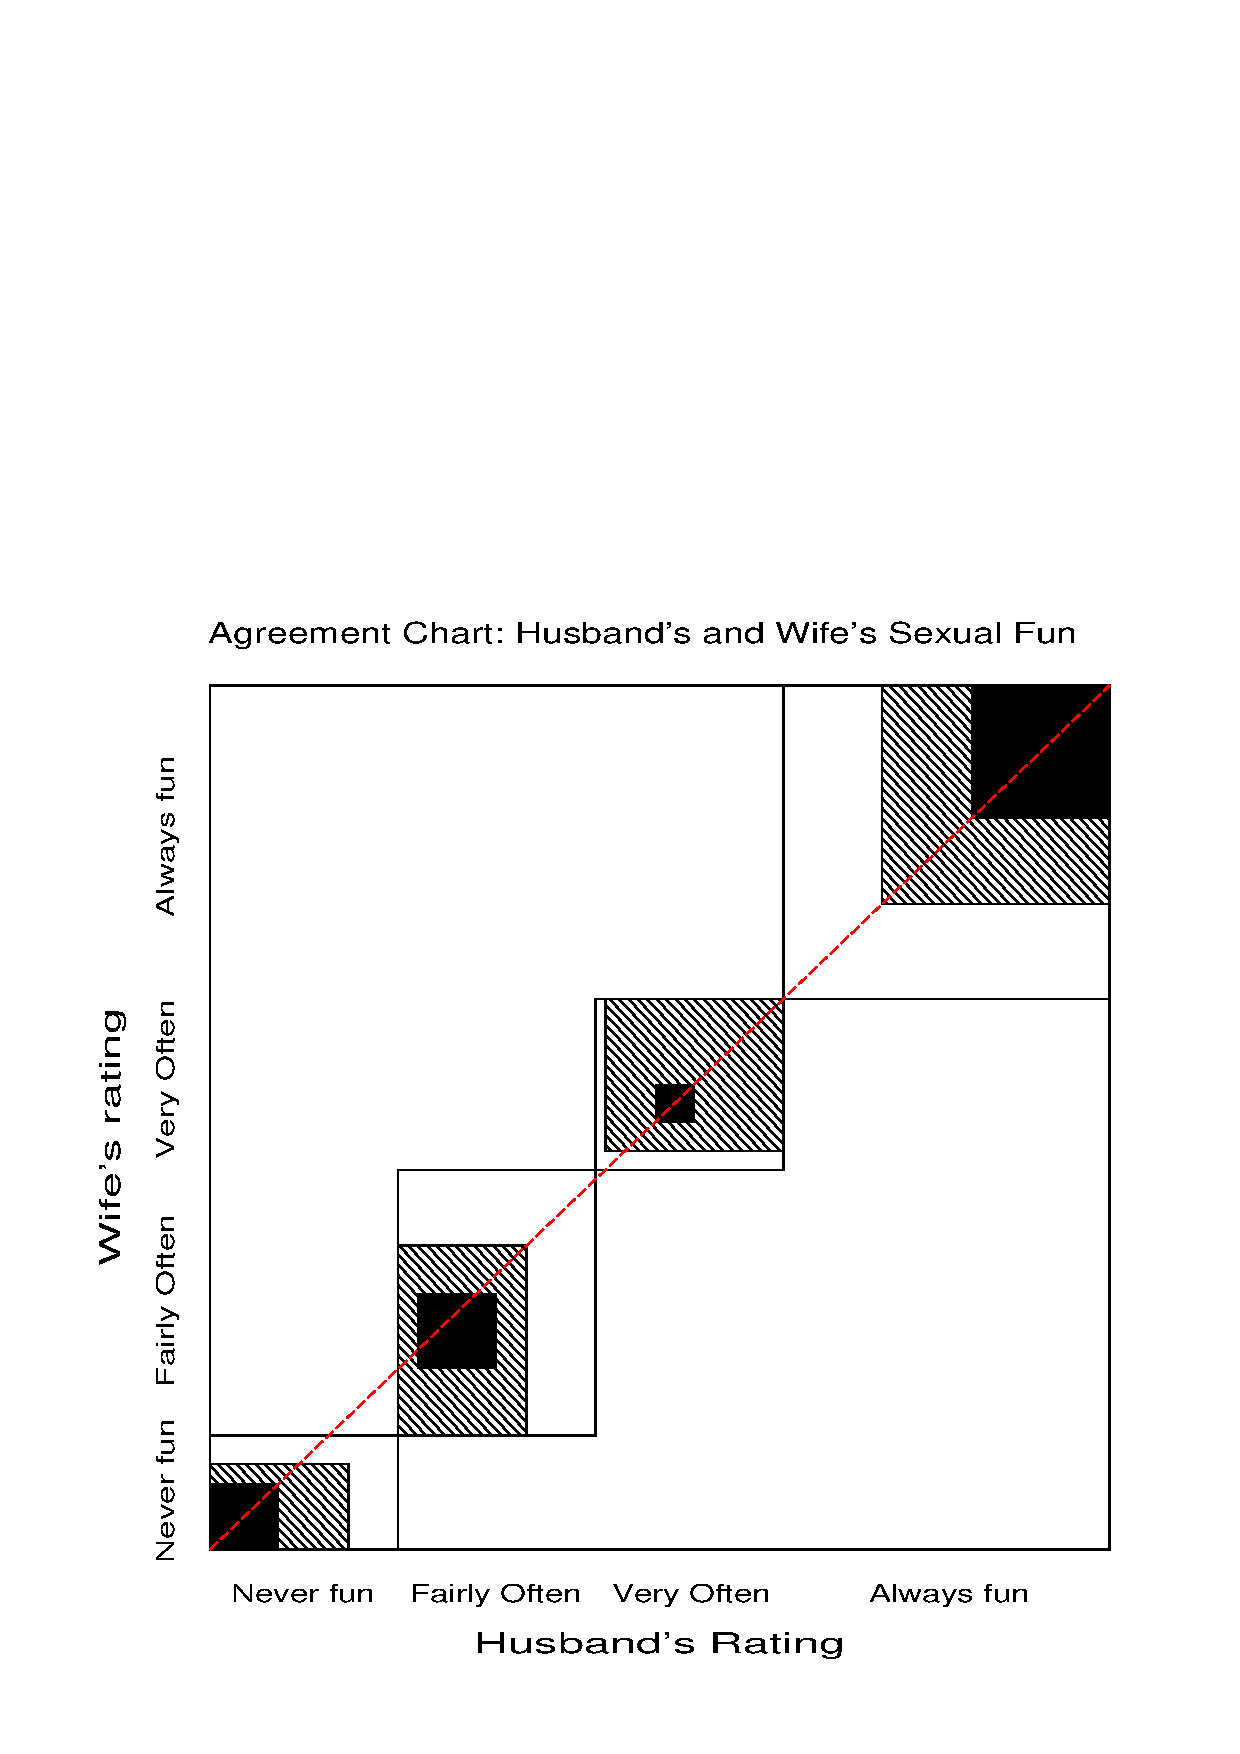
\includegraphics[scale=.5]{ch3/fig/agree12}
  \caption[Weighted agreement chart]{Weighted agreement chart.  The
\(B_N^w\) measure is the ratio of the areas of the dark squares to
their enclosing rectangles, weighting cells one step removed from
exact agreement with \(w_1 = 8 / 9 = .889\).  \(B_N^w  =
0.628\) for these data.}\label{fig:agree12}
\end{figure}

\subsection{Observer bias}\label{sec:Observer}

With an ordered scale, it may happen that one observer consistently
tends to classify the objects into higher or lower categories than
the other.  This produces differences in the marginal totals,
\(n_{i+}\), and \(n_{+i}\).  While special tests exist for
\boldital{marginal homogeneity}, the observer agreement chart shows this
directly by the relation of the dark squares to the diagonal line:
When the marginal totals are the same, the squares fall along the
diagonal.
\ix{marginal homogeneity}

\begin{Example}[MS2]{Diagnosis of MS patients}
\tabref{tab:msdiag} shows the classification of
69 New Orleans patients regarding multiple sclerosis diagnosis by
neurologists in New Orleans and Winnipeg.  The complete \Dset,
listed in \datref{dat:msdiag}, also includes 149 Winnipeg patients who
were assessed by both neurologists.

It is instructive to compare the agreement charts for the two patient
samples, shown in
\figref{fig:agree2}.
For both groups of patients,
the two intermediate categories lie largely above the line,
indicating that the Winnipeg neurologist tends to classify patients
into more severe diagnostic categories.
The departure from the diagonal is greater for the Winnipeg patients,
for whom the Winnipeg neurologist uses the two most severe diagnostic
categories very often.
\ixd{multiple sclerosis diagnosis}

\begin{figure}[htb]
  \centering
  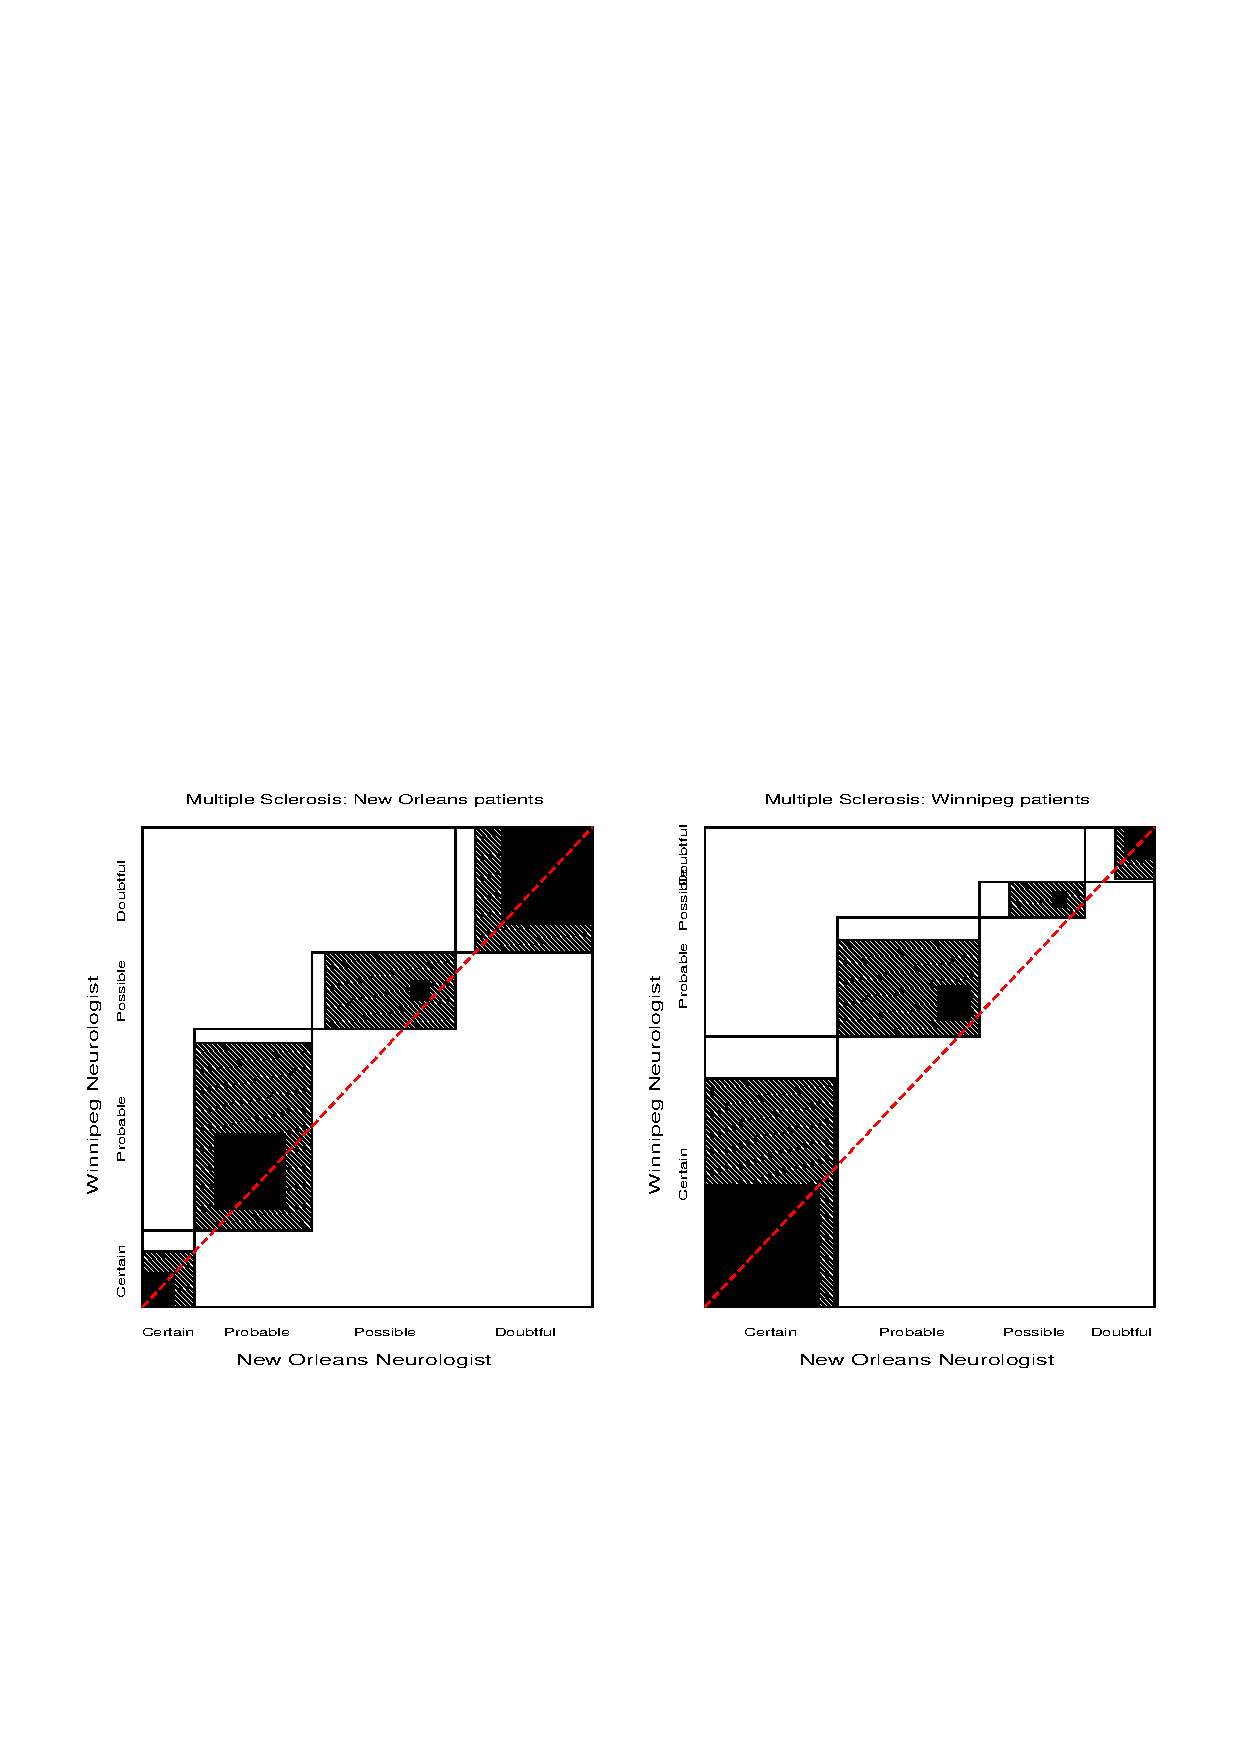
\includegraphics[width=1\linewidth,clip]{ch3/fig/agree2}
  \caption[Weighted agreement chart]{Weighted agreement chart for the MS data.  Departure of the middle squares from the diagonal indicates lack of marginal homogeneity.}\label{fig:agree2}
\end{figure}
\end{Example}

\subsection{The \sasprog{AGREE}}
The observer agreement charts are produced by the \sasprog{AGREE},
which is listed and described in \macref{mac:agree}.
It is written in \IML{} and so is used like the \sasprog{SIEVE}:
\begin{listing}
run agree(table,w, vnames, lnames, title);
\end{listing}

In addition to the \texttt{TABLE}, \texttt{VNAMES}, and \texttt{LNAMES}
arguments,
the \texttt{AGREE} module takes a vector \texttt{W} of one or more weights
to specify the number of steps of disagreement, and the weight to be
applied to each.
The following statements produce \figref{fig:agree11} and
\figref{fig:agree12}.
In the first call to \texttt{AGREE}, \texttt{w=1}, so only exact
agreement is considered; in the second call, \texttt{w=\{1 .889\}},
so 1-step disagreements are given weights of $\frac89$.
%% input: /users/faculty/friendly/sasuser/catdata/agree1.sas
%% last modified: 15-Jan-98 15:25
\begin{listing}
title "Observer Agreement Chart";
proc iml;
   %include agree;
   table =
     \{  7     7     2      3,
        2     8     3      7,
        1     5     4      9,
        2     8     9     14 \};
   title  = "Agreement Chart: Husband's and Wife's Sexual Fun";
   vnames = \{"Husband's Rating" "Wife's rating"\};
   lnames = \{'Never fun' 'Fairly Often' 'Very Often' 'Always fun'\} ;
   font = 'hwpsl009';
   
   w=1;                     /* \figref{fig:agree11} */
   run agree(table, w, vnames, lnames, title);
   w = w || (8/9);          /* \figref{fig:agree12} */
   run agree(table, w, vnames, lnames, title);
   end;
quit;
\end{listing}

\ix{observer agreement chart|)}
\ix{agreement!observer agreement chart|)}

\section{Correspondence analysis}
\renewcommand{\FileName}{corresp}
\subsection{Basic ideas}
\begin{frame}[squeeze]
  \frametitle{Correspondence analysis}
  \begin{block}{\large\bfseries Correspondence analysis (CA)} 
     Analog of PCA for frequency data: 
      \begin{itemize*}
	  \item account for maximum \% of $\chi^2$ in few (2-3) dimensions
	  \item finds scores for row ($x_{im}$) and column ($y_{jm}$) categories on these dimensions
	  \item uses Singular Value Decomposition of residuals from independence,
	  $d_{ij} = (n_{ij} - \widehat{m}_{ij}) / \sqrt{\widehat{m}_{ij}}$
\begin{equation*}
  \frac{  d_{ij}} { \sqrt { n } }
 = \sum_{m=1}^M  \lambda_m \,  x_{im} \,  y_{jm}
\end{equation*}
	  \item \emph{optimal scaling}:  each pair of scores for rows ($x_{im}$) and columns ($y_{jm}$) have highest
	  possible correlation ($= \lambda_m$).
	  \item plots of the row ($x_{im}$) and column ($y_{jm}$) scores show associations
	  \end{itemize*}
  \end{block}
\end{frame}


\begin{frame}
Hair color, Eye color data:
 \begin{center}
  \includegraphics[height=.72\textheight,clip]{fig/corresp2a}
  \begin{itemize*}
  \item Interpretation:  row/column points ``near'' each other are positively associated
  \item Dim 1: 89.4\% of $\chi^2$ (dark $\leftrightarrow$ light)
  \item Dim 2: 9.5\% of $\chi^2$ (RED/Green vs.\ others)
  \end{itemize*}
 \end{center}
\end{frame}

\begin{frame}[fragile]
  \frametitle{\PROC{CORRESP} and the \macrot{CORRESP}}
  \begin{itemize}
	\item Two forms of input \Dset:
      \begin{itemize*}
	  \item \Dset\ in \emph{contingency table} form -- column variables are levels of one factor,
	  observations (rows) are levels of the other.
\begin{listing}[frame=single,baselinestretch=0.9]
Obs     Eye     BLACK    BROWN    RED    BLOND

 1     Brown      68      119      26       7 
 2     Blue       20       84      17      94 
 3     Hazel      15       54      14      10 
 4     Green       5       29      14      16 
\end{listing}

	  \item Raw category responses (\emph{case form}), or cell frequencies (\emph{frequency form}),
	  classified by 2 or more factors (e.g., output from \PROC{FREQ})
\begin{listing}[frame=single,baselinestretch=0.9]
Obs     Eye     HAIR      Count

  1    Brown    BLACK       68
  2    Brown    BROWN      119
  3    Brown    RED         26
  4    Brown    BLOND        7
  ...
 15    Green    RED         14
 16    Green    BLOND       16
\end{listing}
	  \end{itemize*}
  \end{itemize}

\end{frame}

\begin{frame}
  \frametitle{Software: \PROC{CORRESP}, \macrot{CORRESP} \& R}
  \begin{itemize}
	\item<-1>{\large\bfseries \PROC{CORRESP}}
      \begin{itemize*}
	  \item Handles 2-way CA, extensions to \nway\ tables, and MCA
	  \item Many options for scaling row/column coordinates and output statistics
	  \item \texttt{OUTC=} option $\rightarrow$ \ODS\ for plotting
	  \item  SAS V9.1+: \PROC{CORRESP} uses ODS Graphics
      \end{itemize*}
	  
	\item<2->{\large\bfseries \macro{CORRESP}}
      \begin{itemize*}
	  \item Uses \PROC{CORRESP} for analysis
	  \item Produces labeled plots of the category points in either 2 or 3 dimensions
	  \item Many graphic options; can equate axes automatically
	  \item See: \url{http://datavis.ca/sasmac/corresp.html}
      \end{itemize*}

	\item<3->{\large\bfseries \proglang{R}}
      \begin{itemize*}
     \item The \pkg{ca} provides 2-way CA, MCA and more
	 \item \texttt{plot(ca(data))} gives reasonable (but not yet beautiful) plots
	 \item Other R packages: caGUI, vegan, ade4, FactoMiner, ...
      \end{itemize*}
 \end{itemize}

\end{frame}

\begin{frame}[fragile]
  \frametitle{Example: Hair and Eye Color}
  \begin{itemize}
	\item {\large\bfseries Input the data} in contingency table form

\vspace{2ex}
\begin{Input}[label=\fbox{\texttt{corresp2a.sas} $\cdots$},baselinestretch=0.9]
data haireye;
  input  EYE $ BLACK BROWN RED BLOND ; \ignore{$}
  datalines;
        Brown    68   119    26     7    
        Blue     20    84    17    94    
        Hazel    15    54    14    10    
        Green     5    29    14    16    
;
\end{Input}
  \end{itemize}
\end{frame}

\begin{frame}[fragile]
  \frametitle{Example: Hair and Eye Color}

  \begin{itemize}
	\item{\large\bfseries Using \PROC{CORRESP} directly}--- ODS graphics (V9.1+)
\begin{Input}[baselinestretch=0.9,numbers=none]
ods rtf; \sascomment{/* ODS destination: rtf, html, latex, ... */}
\sasemph{ods graphics on;}
proc corresp data=haireye short;
  id eye;                         \sascomment{/* row variable  */}
  var black brown red blond;      \sascomment{/* col variables */}
\sasemph{ods graphics off;}
ods rtf close;
\end{Input}
	\item{\large\bfseries Using the \macro{CORRESP}}--- labeled high-res plot
\begin{Input}[baselinestretch=0.9,numbers=none]
%corresp (data=haireye, 
    id=eye,                     \sascomment{/* row variable  */}
    var=black brown red blond,  \sascomment{/* col variables */}
    dimlab=Dim);                \sascomment{/* options       */}
\end{Input}
  \end{itemize}
\end{frame}

\begin{frame}[fragile]
  \frametitle{Example: Hair and Eye Color}
Printed output:
\begin{Output}[fontsize=\footnotesize,baselinestretch=0.7,gobble=5]
                    The Correspondence Analysis Procedure

                     Inertia and Chi-Square Decomposition

       Singular  Principal Chi-
       Values    Inertias  Squares Percents   18   36   54   72   90
                                           ----+----+----+----+----+---
       0.45692   0.20877   123.593  89.37% *************************
       0.14909   0.02223    13.158   9.51% ***
       0.05097   0.00260     1.538   1.11%
                 -------   -------
                 0.23360    138.29 (Degrees of Freedom = 9)

                               Row Coordinates
                                     Dim1          Dim2

                      Brown      -.492158      -.088322
                      Blue       0.547414      -.082954
                      Hazel      -.212597      0.167391
                      Green      0.161753      0.339040

                              Column Coordinates
                                     Dim1          Dim2

                      BLACK      -.504562      -.214820
                      BROWN      -.148253      0.032666
                      RED        -.129523      0.319642
                      BLOND      0.835348      -.069579
\end{Output}
\end{frame}

\begin{frame}[fragile]
  \frametitle{Example: Hair and Eye Color}
Output \Dset (selected variables):
\begin{Output}[fontsize=\footnotesize,baselinestretch=0.8,gobble=3]
     Obs    _TYPE_      EYE       DIM1        DIM2

      1     INERTIA               .           .
      2     OBS        Brown    -0.49216    -0.08832
      3     OBS        Blue      0.54741    -0.08295
      4     OBS        Hazel    -0.21260     0.16739
      5     OBS        Green     0.16175     0.33904
      6     VAR        BLACK    -0.50456    -0.21482
      7     VAR        BROWN    -0.14825     0.03267
      8     VAR        RED      -0.12952     0.31964
      9     VAR        BLOND     0.83535    -0.06958
\end{Output}
Row and column points are distinguished by the \verb|_TYPE_| variable: \texttt{OBS} vs.\ \texttt{VAR}
\end{frame}

\begin{frame}
  \frametitle{Example: Hair and Eye Color}
Graphic output from \macro{CORRESP}:
 \begin{center}
  \includegraphics[height=.72\textheight,clip]{fig/corresp2a}
%   \begin{itemize*}
%   \item Top legend produced with Annotate data set and the \texttt{INANNO=} option to the \macro{CORRESP}
%   \end{itemize*}
 \end{center}
\end{frame}

\subsection{CA in R}
\renewcommand{\FileName}{ca-R}

\begin{frame}[fragile]
	\frametitle{CA in R: the \pkg{ca}}

\begin{Rin}[baselinestretch=0.8,fontsize=\footnotesize]
> HairEye <- margin.table(HairEyeColor, c(1, 2))
> library(ca)
> ca(HairEye)
\end{Rin}
%Printed output:
\begin{Rout}[baselinestretch=0.8,fontsize=\footnotesize]
 Principal inertias (eigenvalues):
           1        2        3       
Value      0.208773 0.022227 0.002598
Percentage 89.37%   9.52%    1.11%   
 ...
\end{Rout}
Plot the \texttt{ca} object:
\begin{Rin}
> plot(ca(HairEye), main="Hair Color and Eye Color")
\end{Rin}

\begin{center}
\includegraphics[height=.46\textheight,trim=5 20 5 10]{fig/ca-haireye}
\end{center}
\end{frame}

\subsection{Multi-way tables}
\begin{frame}
  \frametitle{Multi-way tables}
Correspondence analysis can be extended to $n$-way tables in several ways:
  \begin{itemize}
	\item<1-> {\large\bfseries Multiple correspondence analysis (MCA)} 
		\begin{itemize*}
     	  \item Extends CA to $n$-way tables
          \item only uses bivariate associations 
		\end{itemize*}

    \item<2-> {\large\bfseries Stacking approach}
 		\begin{itemize*}
         \item $n$-way table flattened to a 2-way table, combining several variables ``interactively''
		 \item Each way of stacking corresponds to a \emph{\loglin\ model}
         \item Ordinary CA of the flattened table $\rightarrow$ visualization of that model
         \item Associations among stacked variables are \emph{not visualized}
		\end{itemize*}
	\item<3-> Here, I only describe the stacking approach, and only with SAS
		\begin{itemize*}
		\item In SAS 9.3, the \texttt{MCA} option with \PROC{CORRESP} provides some reasonable plots.
		 \item For R, see the \pkg{ca}-- the \func{mjca} function is much more general
		\end{itemize*}

   \end{itemize}
\end{frame}

\begin{frame}<none>
  \frametitle{Multi-way tables}
  \begin{itemize}
	\item{\large\bfseries Stacking approach:} \citet{HeijdenLeeuw:85}--- 
      \begin{itemize*}
	  \item three-way table, of size \(I \times  J \times  K\) can be sliced and stacked as
	a two-way table, of size \((I \times  J ) \times  K\)
 \begin{center}
  \includegraphics[height=.45\textheight,clip]{fig/stacking}
 \end{center}

	  \item The variables combined are treated ``interactively''
	  \item Each way of stacking corresponds to a \loglin\ model
    	\begin{itemize*}
		\item \((I \times  J ) \times  K\) $\rightarrow$ [AB][C]
		\item \(I \times  ( J \times  K )\) $\rightarrow$ [A][BC]
		\item \(J \times  ( I \times  K )\) $\rightarrow$ [B][AC]
		\end{itemize*}
	  \item Only the associations in separate [] terms are analyzed and displayed
	  \end{itemize*}
  \end{itemize}
\end{frame}

\begin{frame}
  \frametitle{Multi-way tables: Stacking}
  \begin{itemize}
	\item{\large\bfseries Stacking approach:} \citet{HeijdenLeeuw:85}--- 
      \begin{itemize*}
	  \item three-way table, of size \(I \times  J \times  K\) can be sliced and stacked as
	a two-way table, of size \((I \times  J ) \times  K\)
 	  \end{itemize*}
 \end{itemize}

 \begin{minipage}[c]{.49\linewidth}
  \includegraphics[width=1\linewidth,clip]{fig/stacking}
 \end{minipage}%
 \hfill
 \begin{minipage}[c]{.49\linewidth}
       \begin{itemize*}
	  \item The variables combined are treated ``interactively''
	  \item Each way of stacking corresponds to a \loglin\ model
    	\begin{itemize*}
		\item \((I \times  J ) \times  K\) $\rightarrow$ [AB][C]
		\item \(I \times  ( J \times  K )\) $\rightarrow$ [A][BC]
		\item \(J \times  ( I \times  K )\) $\rightarrow$ [B][AC]
		\end{itemize*}
	  \item Only the associations in separate [] terms are analyzed and displayed
	  \end{itemize*}
\end{minipage}
\end{frame}

\begin{frame}[fragile]
  \frametitle{Multi-way tables: Stacking}
  \begin{itemize}
	\item{\large\bfseries \PROC{CORRESP}}:  Use \texttt{TABLES} statement and option
	\texttt{CROSS=ROW} or \texttt{CROSS=COL}.  E.g., for model [A B] [C],
\begin{listing}
proc corresp cross=row;
   tables A B, C;
   weight count;
\end{listing}

	\item{\large\bfseries \macro{CORRESP}}: Can use \verb|/| instead of \verb|,|
\begin{listing}
%corresp(
   options=cross=row,
   tables=A B/ C,
   weight count);
\end{listing}
  \end{itemize}

\end{frame}

\begin{frame}[fragile]
  \frametitle{Example: Suicide Rates}
Suicide rates in West Germany, by Age, Sex and Method of suicide
\begin{Output}[baselinestretch=0.9]
   Sex  Age    POISON     GAS    HANG   DROWN     GUN    JUMP

    M  10-20     1160     335    1524      67     512     189
    M  25-35     2823     883    2751     213     852     366
    M  40-50     2465     625    3936     247     875     244
    M  55-65     1531     201    3581     207     477     273
    M  70-90      938      45    2948     212     229     268

    F  10-20      921      40     212      30      25     131
    F  25-35     1672     113     575     139      64     276
    F  40-50     2224      91    1481     354      52     327
    F  55-65     2283      45    2014     679      29     388
    F  70-90     1548      29    1355     501       3     383
\end{Output}
  \begin{itemize}
	\item CA of the [Age Sex] by [Method] table:
      \begin{itemize*}
	  \item Shows associations between the Age-Sex combinations and Method
	  \item Ignores association between Age and Sex
	  \end{itemize*}
  \end{itemize}
\end{frame}

\begin{frame}[fragile]
  \frametitle{Example: Suicide Rates}
\vspace{2ex}
\begin{Input}[label=\fbox{\texttt{suicide5.sas} $\cdots$},baselinestretch=0.9]
%include catdata(suicide);
   \sascomment{*-- equate axes!;}
axis1 order=(-.7 to .7 by .7) length=6.5 in label=(a=90 r=0);
axis2 order=(-.7 to .7 by .7) length=6.5 in;
%corresp(data=suicide,  weight=count,
    \sasemph{tables=%str(age sex, method)}, 
    \sasemph{options=cross=row} short, 
    vaxis=axis1, haxis=axis2);
\end{Input}
Output:
\begin{Output}[fontsize=\footnotesize,baselinestretch=0.8]
                   Inertia and Chi-Square Decomposition

     Singular  Principal Chi-
     Values    Inertias  Squares Percents   12   24   36   48   60
                                         ----+----+----+----+----+---
     0.32138   0.10328   5056.91  60.41% *************************
     0.23736   0.05634   2758.41  32.95% **************
     0.09378   0.00879    430.55   5.14% **
     0.04171   0.00174     85.17   1.02%
     0.02867   0.00082     40.24   0.48%
               -------   -------
               0.17098   8371.28 (Degrees of Freedom = 45)
\end{Output}
\end{frame}

\begin{frame}
CA Graph:
 \begin{center}
  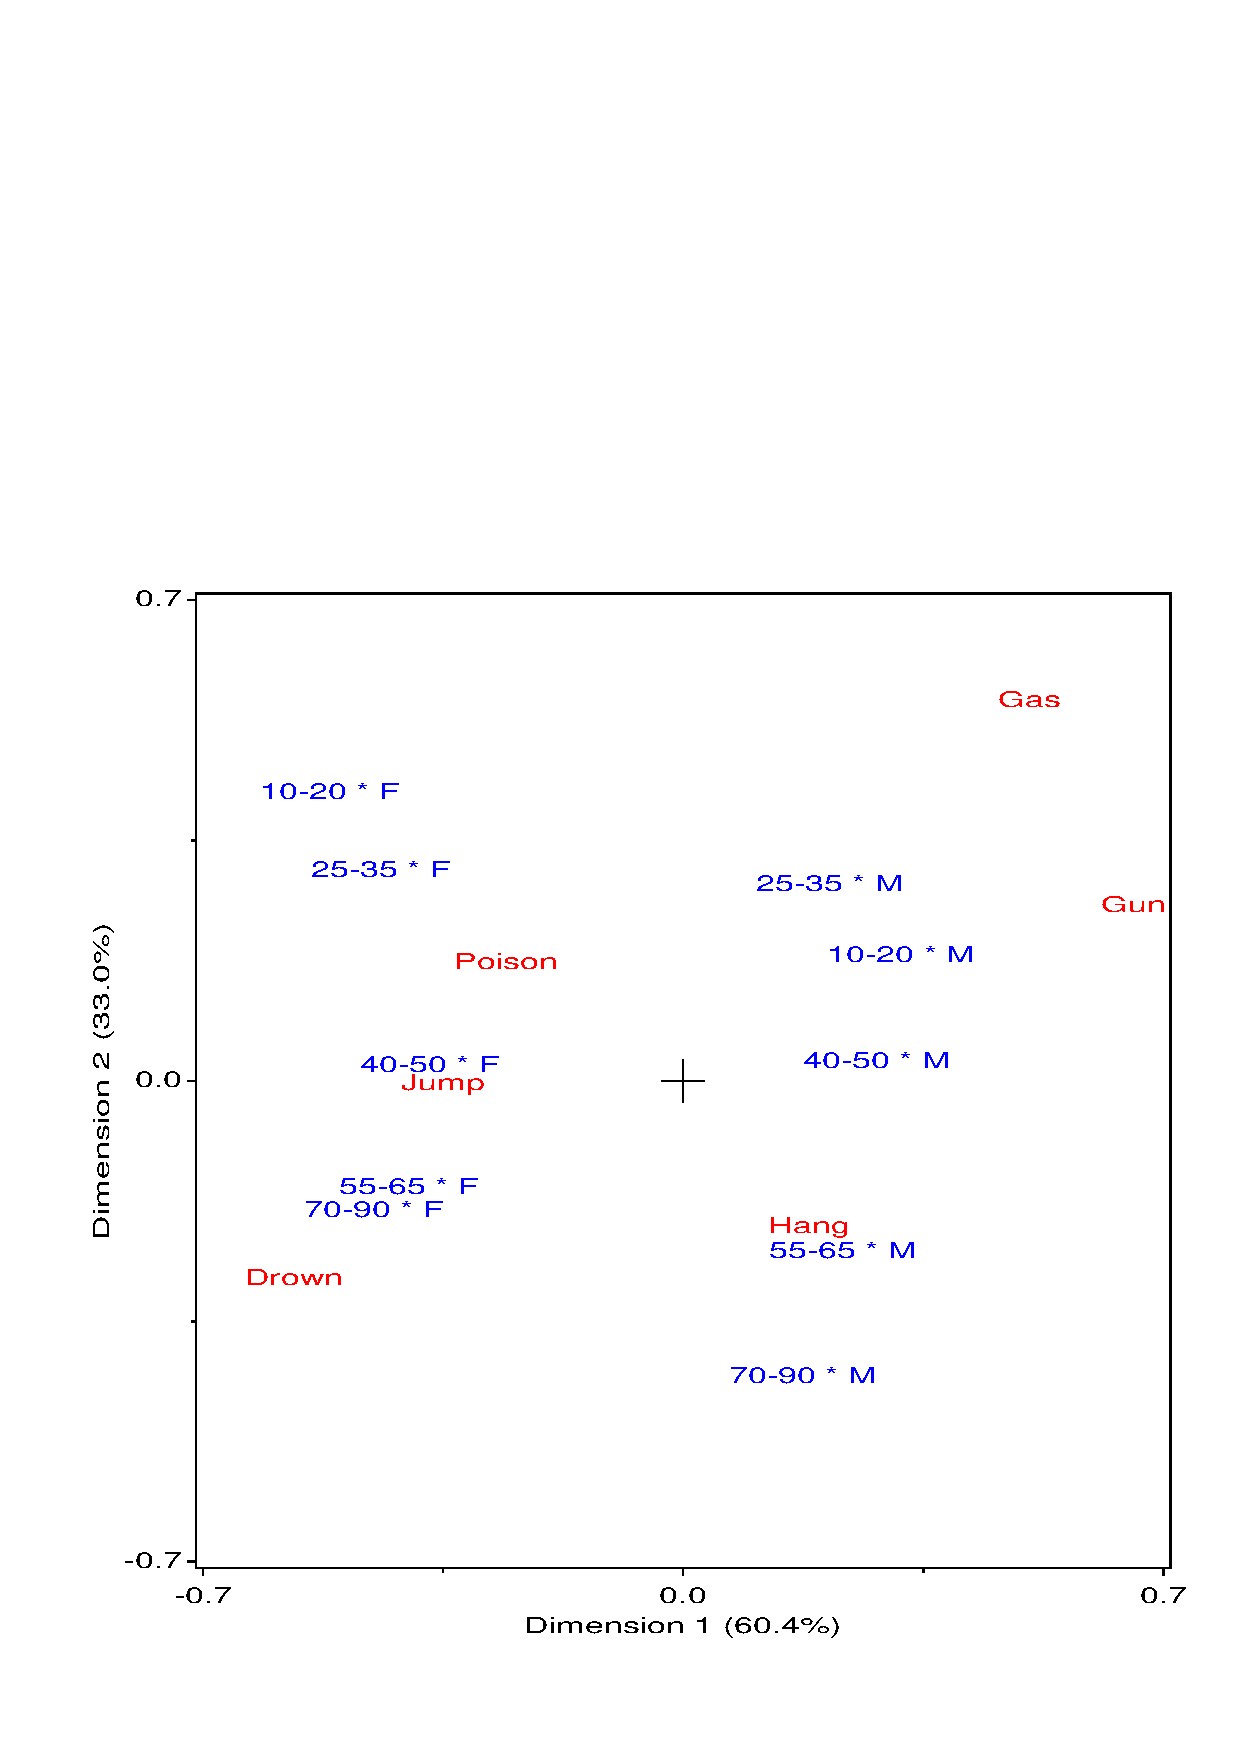
\includegraphics[height=.9\textheight,clip]{fig/suicide51}
 \end{center}
\end{frame}

\begin{frame}
Looking forward--- View this as a mosaic display:
 \begin{center}
  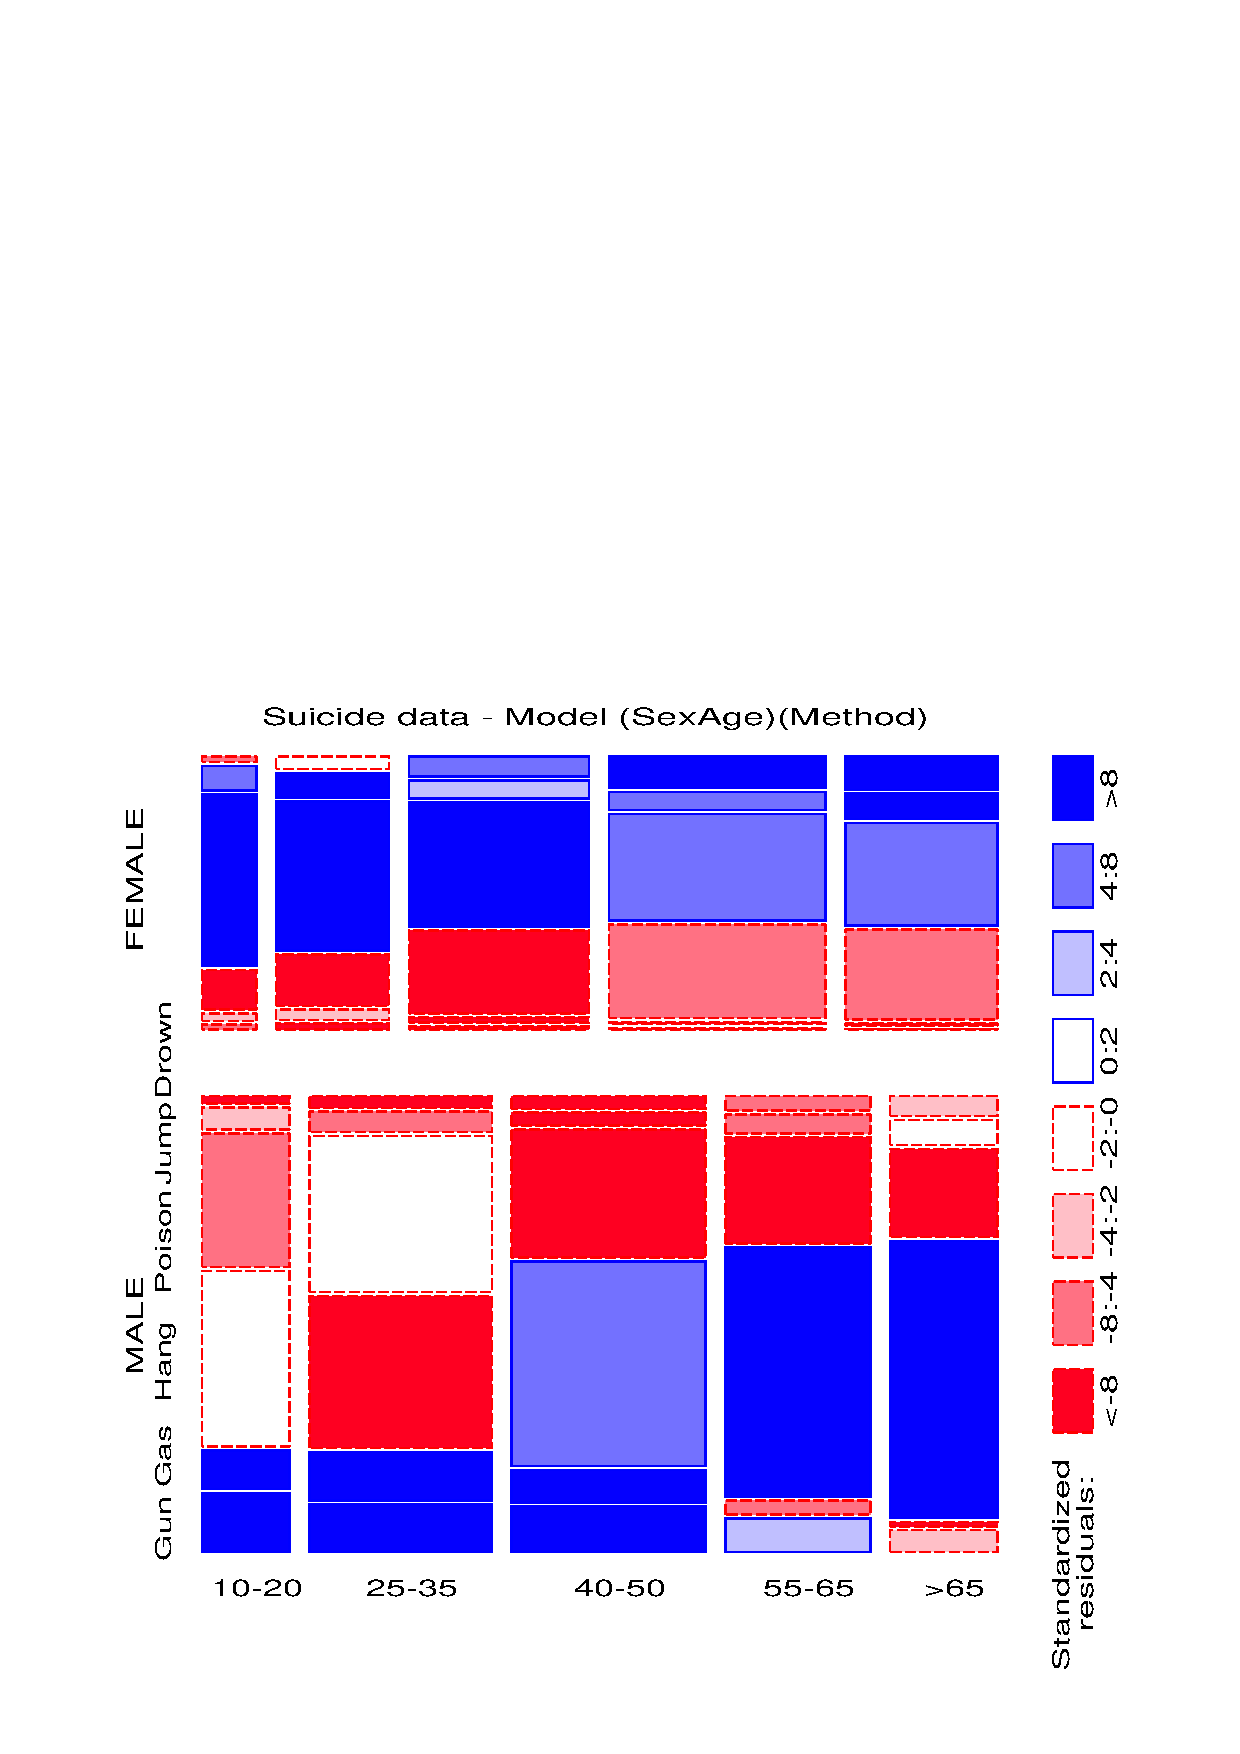
\includegraphics[height=.9\textheight,clip]{fig/mosaic6b}
 \end{center}
\end{frame}

\endinput
% slide template
\begin{frame}
  \frametitle{}
  \begin{itemize}
	\item{\large\bfseries }
      \begin{itemize*}
	  \item 
    	\begin{itemize*}
		\item 
		\item 
		\end{itemize*}
	  \item 
	  \end{itemize*}
	\item{\large\bfseries }
	\item{\large\bfseries }
  \end{itemize}
\end{frame}


\section{Summary: Part 2}
\renewcommand{\FileName}{summary2}
% slide template
\begin{frame}
  \frametitle{Summary: Part 2}
  \begin{itemize}
	\item<+->{\large\bfseries Fourfold displays}
      \begin{itemize*}
	  \item Odds ratio: ratio of areas of diagonally opposite quadrants
	  \item Confidence rings: visual test of $H_0: \theta = 1$
	  \item Shading: highlight strata for which $H_a: \theta \ne 1$
	  \end{itemize*}
	\item<+->{\large\bfseries Sieve diagrams}
      \begin{itemize*}
	  \item  Rows and columns $\sim$ marginal frequencies $\rightarrow$ area $\sim$ expected
 	  \item  Shading $\sim$ observed frequencies
	  \item  Simple visualization of pattern of association
	  \item SAS: \macro{sieveplot}; R: \func{sieve}
	  \end{itemize*}
	\item<+->{\large\bfseries Agreement}
     \begin{itemize*}
	  \item Cohen's $\kappa$: strength of agreement
 	  \item Agreement chart: visualize weighted \& unweighted agreement, marginal homogeneity
      \item SAS: \macro{agreeplot}; R: \func{agreementplot}
	  \end{itemize*}
 	\item<+->{\large\bfseries Correspondence analysis}
     \begin{itemize*}
	  \item Decompose $\chi^2$ for association into 1 or more dimensions
 	  \item $\rightarrow$ scores for row/col categories
	  \item CA plots: Interpretation of \emph{how} the variables are related
      \item SAS: \macro{corresp}; R: \func{ca}
	  \end{itemize*}
 \end{itemize}
\end{frame}



\endinput
\lecture{n-way tables}{n-way}
\renewcommand{\FileName}{part3}

\part{n-way tables}
\begin{frame}
  \frametitle{Part 3: Mosaic displays and \loglin\ models}
 \begin{minipage}[c]{.33\textwidth}
  \includegraphics[width=1\linewidth]{fig/mosaic9a3f}
  \end{minipage}%
 \hfill
 \begin{minipage}[c]{.33\textwidth}
  \includegraphics[width=1\linewidth,clip]{fig/mosaic9a4f}
 \end{minipage}
 \hfill
 \begin{minipage}[c]{.33\textwidth}
  \includegraphics[width=1\linewidth,clip]{fig/mosmat9m}
 \end{minipage}

Topics:
  \begin{itemize*}
	\item Mosaic displays 
	\item \loglin\ models for \nway\ tables
%	\item Correspondence analysis
    \item Visualizing \loglin\ models: \proglang{SAS} \& \proglang{R}
    \item Models for square and structured tables
	\item Larger tables
  \end{itemize*}
\end{frame}

\section{n-way tables}
\renewcommand{\FileName}{mosbasic}

\subsection{Mosaic displays: Basic ideas}
\begin{frame}
  \frametitle{Mosaic displays: Basic ideas}
\citet{HartiganKleiner:81,Friendly:94a,Friendly:99b}
 \begin{columns}
   \begin{column}{.5\textwidth}
     \begin{itemize}
      \item Area-proportional display of frequencies in an $n$-way table
	  \item Tiles (cells): recursive splits of a unit square---
		\begin{itemize*}
		 \item<1-> V1: \alert{width} $\sim$ marginal frequencies, $n_{i++}$
		 \item<2-> V2: \alert{height} $\sim$ relative frequencies \given V1, $n_{ij+} / n_{i++}$
		 \item<3-> V3: \alert{width} $\sim$ relative frequencies \given (V1, V2), $n_{ijk} / n_{ij+}$
         \item<3-> $\cdots$
		\end{itemize*}
       \item $\Rightarrow$  area $\sim$ cell frequency, $n_{ijk}$
     \end{itemize}
   \end{column}
   \begin{column}{.5\textwidth}
      \includegraphics<1>[width=\linewidth]{fig/ucb0}
      \includegraphics<2>[width=\linewidth]{fig/ucb1}
      \includegraphics<3>[width=\linewidth]{fig/ucb4}
   \end{column}
 \end{columns}
\end{frame}


\begin{frame}
  \frametitle{Mosaic displays: Basic ideas}
 \begin{columns}
   \begin{column}{.5\textwidth}
     \begin{itemize}
      \item Independence: Two-way table
	  \item Expected frequencies: 
		\begin{equation*}
		 \widehat{m}_{ij} = \frac{n_{i+} n_{+j}}{n_{++}} = n_{++} \text{row \%} \text{col \%}
		\end{equation*}
       \item $\Rightarrow$  rows \& columns align when variables are independent
     \end{itemize}
   \end{column}
   \begin{column}{.5\textwidth}
      \includegraphics[width=\linewidth]{fig/ucb1e}
   \end{column}
 \end{columns}
\end{frame}

\begin{frame}
  \frametitle{Mosaic displays: Residuals \& shading}
 \begin{columns}
   \begin{column}{.5\textwidth}
     \begin{itemize}
%      \item Independence: Two-way table
	  \item \alert{Pearson residuals}: 
		\begin{equation*}
		 d_{ij} = \frac{n_{ij} - \widehat{m}_{ij} }{\sqrt{\widehat{m}_{ij}}}
		\end{equation*}
       \item Pearson $\chi^2 = \Sigma \Sigma d_{ij}^2 =  \Sigma \Sigma \frac{(n_{ij} - \hat{m}_{ij})^2}{\hat{m}_{ij}}$
       \item Other residuals: deviance (LR), Freeman-Tukey (FT), adjusted (ADJ), ...
       \item \alert{Shading}:
			\begin{itemize*}
			\item Sign: \red{$-$ negative in red}; \blue{$+$ positive in blue}
			\item Magnitude: intensity of shading:  $|d_{ij}| > 0, 2, 4, \dots$
			\end{itemize*}
       \item $\Rightarrow$ Independence:  rows align, or \alert{cells are empty}!
     \end{itemize}
   \end{column}
   \begin{column}{.5\textwidth}
      \includegraphics[width=\linewidth]{fig/ucb2}
   \end{column}
 \end{columns}
\end{frame}

\endinput

\subsection{Loglinear models: Overview}
\renewcommand{\FileName}{loglin}
% slide template
% slide template
\begin{frame}
  \frametitle{\Loglin\  models: Overview}
  \begin{block}{\large\bfseries Modeling perspectives}
      \begin{itemize}[<+->]
	    \item \alert{\Loglin} models can be developed as an analog of classical ANOVA and regression
		models, where \emph{multiplicative} relations (under independence) are re-expressed in \emph{additive}
		form as models for log(frequency).
          \begin{equation*}
          	 	\log m_{ij} = \mu + \lambda_i^A + \lambda_j^B 	\equiv [A] [B] \equiv \sim A + B
          \end{equation*}

		\item More generally, \loglin\ models are also \alert{generalized linear models}
        (GLMs) 
		for log(frequency), with a Poisson distribution for the cell counts.
			\[ \log \vec{m} = \mat{X}  \vec{\beta}\]

		\item When one table variable is a response, a \alert{logit model} for that response is equivalent
		to a \loglin\ model (discussed in Part 4).
          \begin{equation*}
          	 	\log (m_{1jk}/m_{2jk}) = \alpha + \beta_j^B + \beta_k^C	\equiv [AB] [AC] [BC]
          \end{equation*}
      \end{itemize}
  \end{block}
\end{frame}
	
\begin{frame}[allowframebreaks]
  \frametitle{\Loglin\  models: Overview}
  \begin{itemize}
   \item {\large\bfseries Two-way tables: \Loglin\ approach}
%      \begin{itemize*}

      For two discrete variables, $A$ and $B$, suppose a multinomial sample of total size $n$
	  over the $IJ$ cells of a two-way $I \times J$ contingency table, with cell frequencies
	  $n_{ij}$, and cell probabilities $\pi_{ij} = n_{ij}/n$.
    	\begin{itemize*}
	  	\item The table variables are \alert{statistically independent} when the cell (joint) probability equals
	  	the product of the marginal probabilities, $\Pr(A=i \:\&\: B=j) = \Pr(A=i) \times  \Pr(B=j)$, or,
	  	\[ \pi_{ij} = \pi_{i+} \pi_{+j} \period \]
	  	\item An equivalent model in terms of expected frequencies, $m_{ij} = n \pi_{ij}$ is
	  	\[ m_{ij} = (1/n) \: m_{i+} \: m_{+j} \period \]
%\framebreak
		\item This multiplicative model can be expressed in additive form as a model for $\log m_{ij}$,
	\begin{equation}\label{eq:logmij}
	 \log m_{ij} = -\log n + \log m_{i+} + \log m_{+j} \period
	\end{equation}
\framebreak
		\item By anology with ANOVA models, the independence model \eqref{eq:logmij} can be expressed as 
		\begin{equation}\label{eq:independence}
	 	\log m_{ij} = \mu + \lambda_i^A + \lambda_j^B \comma	
		\end{equation}
		where $\mu$ is the grand mean of $\log m_{ij}$ and the parameters $\lambda_i^A$ and  $\lambda_j^B$
		express the marginal frequencies of variables $A$ and $B$, and are typically defined so that
		 $\sum_i \lambda_i^A = \sum_j \lambda_j^B =0$.
		\end{itemize*}

	   Dependence between the table variables is expressed by adding association parameters,
		$\lambda_{ij}^{AB}$, giving the \emph{saturated model},
	\begin{equation}\label{eq:saturated}
	 	\log m_{ij} = \mu + \lambda_i^A + \lambda_j^B + \lambda_{ij}^{AB} \equiv [AB] \equiv \sim
		A*B \period  
	\end{equation}
		\begin{itemize*}
			\item The saturated model fits the table perfectly ($\widehat{m}_{ij} = n_{ij}$): 
			there are as many parameters as cell
			frequencies. Residual df = 0.
			\item A global test for association tests $H_0: \mat{\lambda}_{ij}^{AB} = \mat{0}$.
			\item For ordinal variables, the $\lambda_{ij}^{AB}$ may be structured more simply,
			giving tests for ordinal association.
		\end{itemize*}
%	  \end{itemize*}
  \end{itemize}
	
\end{frame}
%\framebreak
\begin{frame}	
  \begin{itemize}
	\item{\large\bfseries \large\bfseries Two-way tables: GLM approach}
		\begin{itemize}
			\item In the GLM approach, the vector of cell frequencies, $\vec{n} = \{ n_{ij}\}$ is specified
			to have a \alert{Poisson} distribution with means $\mat{m} = \{m_{ij}\}$ given by
			\[ \log \vec{m} = \mat{X}  \vec{\beta}\]
			where $\mat{X}$ is a known design (model) matrix and $\vec{\beta}$ is a column vector
			containing the unknown $\lambda$ parameters.
			\item For example, for
a $2\times 2$ table, the saturated model \eqref{eq:saturated} with the usual zero-sum constraints
can be represented as
\begin{equation*}
\left(
\begin{array}{c}
\log m_{11} \\
\log m_{12} \\
\log m_{21} \\
\log m_{22}
\end{array}
\right) =\left[
\begin{array}{rrrr}
1 & 1 & 1 & 1 \\
1 & 1 & -1 & -1 \\
1 & -1 & 1 & -1 \\
1 & -1 & -1 & 1
\end{array}
\right] \left(
\begin{array}{c}
\mu  \\
\lambda _1^A \\
\lambda _1^B \\
\lambda _{11}^{AB}
\end{array}
\right)
\end{equation*}
Note that only the linearly independent parameters are represented.
$\lambda_2^A = - \lambda_1^A$, because $\lambda_1^A + \lambda_2^A =0$, 
and so forth.
		\item Advantages of the GLM formulation: easier
to express models with ordinal or quantitative variables, special terms, etc. 
Can also allow for \emph{over-dispersion}. 
		\end{itemize} 
%	\item{\large\bfseries }
  \end{itemize}
\end{frame}

% slide template
\begin{frame}[allowframebreaks]
  \frametitle{Three-way Tables}
  \begin{itemize}
	\item{\large\bfseries Saturated model:} For a 3-way table, of size $I \times J \times K$ for variables $A, B, C$,
	 the saturated \loglin\ model includes associations between
	all pairs of variables, as well as a 3-way association term, $\lambda_{ijk}^{ABC}$
\begin{equation} \label{eq:lsat3}
  \begin{split}
  \log \,  m_{ijk}  
 = \mu  
& +  \lambda_i^A
  +  \lambda_j^B
  +  \lambda_k^C       \\
& +  \lambda_{ij}^{AB}
  +  \lambda_{ik}^{AC}
  +  \lambda_{jk}^{BC}
  +  \lambda_{ijk}^{ABC}
  \period
  \end{split}
\end{equation}
      \begin{itemize*}
	  \item One-way terms ($\lambda_i^A, \lambda_j^B, \lambda_k^C$):
	  differences in the \emph{marginal frequencies} of the table variables.
	  \item Two-way terms ($\lambda_{ij}^{AB}, \lambda_{ik}^{AC},\lambda_{jk}^{BC}$)
	  pertain to the \emph{partial association} for each pair of variables, \emph{controlling}
	  for the remaining variable.
	  \item The three-way term, $\lambda_{ijk}^{ABC}$ allows the partial association between any
	  pair of variables to vary over the categories of the third variable.
	  \item Such models are usually \emph{hierarchical}:  the presence of a high-order term, such as
	  $\lambda_{ijk}^{ABC}$ $\rightarrow$  \emph{all} low-order relatives are automatically included.
	  \item Thus, a short-hand notation for a \loglin\ model lists only the high-order terms,
	  i.e., model \eqref{eq:lsat3} $\equiv [ABC]$
%    	\begin{itemize*}
%		\item 
%		\item 
%		\end{itemize*}
	  \end{itemize*}
%\end{frame}
\framebreak
%\begin{frame}	
	\item{\large\bfseries Reduced models:}  

    The usual goal is to fit the \emph{smallest} model
	(fewest high-order terms) that is sufficient to explain/describe the observed frequencies.
%    	\begin{itemize*}
%		\item All representative subset models are shown in the table below
		\input{tab/loglin-3waya}
		Symbolic notation (high-order terms):
		\[  [AB][C] \equiv 
  \log \,  m_{ijk}  =
  \mu  +  \lambda_i^A +  \lambda_j^B  +  \lambda_k^C
  +  \lambda_{ij}^{AB}
		\] 
		\[  [AB][AC] \equiv 
  \log \,  m_{ijk}  =
  \mu  +  \lambda_i^A +  \lambda_j^B  +  \lambda_k^C
  +  \lambda_{ij}^{AB}
  +  \lambda_{ik}^{AC}
		\] 
%		\end{itemize*}

%\end{frame}
\framebreak
%\begin{frame}	
	\item{\large\bfseries Assessing goodness of fit}
    	\begin{itemize}
		\item Goodness of fit of a specified model may be tested by the likelihood ratio $G^2$,
\begin{equation}\label{eq:pgsq}
\GSQ =  2 \sum_i n_i \, \log ( n_i / \widehat{m}_i )
\comma
\end{equation}
		or the Pearson $\chisq$,
\begin{equation}\label{eq:pchi}
\chisq = \sum_i \frac{( n_i - \widehat{m}_i )^2}{\widehat{m}_i}
\comma
\end{equation}
	with degrees of freedom = \# cells - \#  estimated parameters.  
	\item E.g., for the model
	of mutual independence, $[A] [B] [C]$, df = $IJK - (I-1) - (J-1) - (K-1) = (I-1)(J-1)(K-1)$
	\item The terms summed in \eqref{eq:pgsq} and \eqref{eq:pchi} are the squared \emph{cell residuals}
	\item Other measures of balance goodness of fit against parsimony, e.g., \emph{Akaike's Information Criterion}
	(smaller is better)
	\[ AIC = \GSQ - 2 df \mbox{ or }  AIC = \GSQ + 2 \mbox{ \# parameters} \]
		\end{itemize}
  \end{itemize}
\end{frame}

\endinput

% slide template
\begin{frame}
  \frametitle{}
  \begin{itemize}
	\item{\large\bfseries }
      \begin{itemize*}
	  \item 
    	\begin{itemize*}
		\item 
		\item 
		\end{itemize*}
	  \item 
	  \end{itemize*}
	\item{\large\bfseries }
	\item{\large\bfseries }
  \end{itemize}
\end{frame}


\subsection{Loglinear models: Fitting}
\renewcommand{\FileName}{loglfit}
\begin{frame}[fragile]
 \frametitle{Fitting \loglin\ models: SAS}
 \begin{block}{SAS}
  \begin{itemize}
   \item \PROC{CATMOD}
\begin{Input}[baselinestretch=0.8,fontsize=\footnotesize]
%include catdata(berkeley);
proc catmod order=data data=berkeley;
   format dept dept. admit admit.;
   \sasemph{weight freq;}                  \sascomment{/* data in freq. form */}
   model dept*gender*admit=_response_ ;
   \sasemph{loglin} admit|dept|gender @2   / title='Model (AD,AG,DG)'; run;
   \sasemph{loglin} admit|dept dept|gender / title='Model (AD,DG)';  run;
\end{Input}

   \item \PROC{GENMOD}
\begin{Input}[baselinestretch=0.8,fontsize=\footnotesize]
proc genmod data=berkeley;
   class dept gender admit;
   model freq = dept|gender dept|admit / \sasemph{dist=poisson};
run;
\end{Input}

  \end{itemize}
 \end{block}
\begin{itemize*}
  \item \texttt{mosaic} macro usually fits loglin models internally and
  displays results
  \item You can also use \PROC{GENMOD} for a more general model, and
  display the result with the \texttt{mosaic} macro.
\end{itemize*}
  
\end{frame}

\begin{frame}[fragile]
 \frametitle{Fitting \loglin\ models: R}
 \begin{block}{R}
  \begin{itemize}
   \item \func{loglm} - data in contingency table form (\pkg{MASS})
\begin{Input}[baselinestretch=0.8,fontsize=\footnotesize]
data(UCBAdmissions)
  ## conditional independence (AD, DG) in Berkeley data
mod.1 <- loglm(~ (Admit + Gender) * Dept, data=UCBAdmissions)
  ## all two-way model (AD, DG, AG) 
mod.2 <- loglm(~ (Admit + Gender + Dept)^2, data=UCBAdmissions)
\end{Input}

   \item \func{glm} - data in frequency form
\begin{Input}[baselinestretch=0.8,fontsize=\footnotesize]
berkeley <- as.data.frame(UCBAdmissions)
mod.3 <- glm(Freq ~ (Admit + Gender) * Dept, data=berkeley, 
                   \sasemph{family='poisson'})
\end{Input}

  \end{itemize}
 \end{block}

\begin{itemize*}
  \item \func{loglm} simpler for nominal variables
  \item \func{glm} allows a wider class of models
  \item \func{gnm} fits models for structured association and
  generalized \emph{non-linear} models
  \item \texttt{vcdExtra} package provides visualizations for all.
  
\end{itemize*}

\end{frame}


\subsection{Mosaic displays}
\renewcommand{\FileName}{nway2}

% these two frames covered in mosbasic
\begin{comment}
\begin{frame}
%\makeatletter\slidebox@restore\makeatother
\frametitle{Mosaic displays and Log-linear Models}
\citet{HartiganKleiner:81,Friendly:94a,Friendly:99b}:
\begin{itemize}
\item \boldital{Width} $\sim$ one set of marginals, $n_{i+}$
\item \boldital{Height} $\sim$ relative proportions of other variable, 
$p_{j\given i} = n_{ij} / n_{i+}$
\item $\Rightarrow$ \textbf{area} $\sim$ \textbf{frequency}, $n_{ij} = n_{i+} p_{j\given i}$
\begin{center}
  \includegraphics[width=.5\dispwidth,clip]{fig/mosaic9a1f}
\end{center}
\end{itemize}
\end{frame}

\begin{frame}
\begin{itemize}
\item \boldital{Shading}: Sign and magnitude of Pearson
$\chi^2$ residual,
$d_{ij} = ( n_{ij} - \hat{m}_{ij} ) / \sqrt{\hat{m}_{ij}}$ (or L.R. $G^2$)
\begin{itemize*}
\item Sign: \red{$-$ negative in red}; \blue{$+$ positive in blue}\black
\item Magnitude: intensity of shading:  $|d_{ij}| > 0, 2, 4, \dots$
\end{itemize*}
\item \boldital{Independence}: Rows $\approx$ align, \emph{or}
cells are empty!
\item E.g., aggregate Berkeley data, independence model:
\end{itemize}

\begin{center}
  \includegraphics[width=.5\dispwidth,clip]{fig/mosaic9a1f}
\end{center}
\end{frame}
\end{comment}

\begin{frame}
  \frametitle{Mosaic displays: Hair color and eye color}
  \vspace{2ex}
 \begin{minipage}[c]{.49\dispwidth}
  \includegraphics[width=1\linewidth,clip]{fig/mosaic3m1}
 \end{minipage}%
 \hfill
 \begin{minipage}[c]{.49\dispwidth}
  We know that hair color and eye color are associated ($\chi^2 (9) = 138.29$).
  The question is \alert{how}?
  \begin{itemize}
  \item Dark hair goes with dark eyes, light hair with light eyes
  \item Red hair, hazel eyes an exception?
  \item Effect ordering: Rows/cols permuted by CA Dimension 1
  \item[$\Rightarrow$] Opposite corner pattern
  \end{itemize}
 \end{minipage}
\end{frame}

\begin{frame}
\frametitle{Mosaic displays: Marginal models}
Berkeley data: Departments $\times$ Gender (ignoring Admit):
\begin{itemize}
\item Did departments differ in the total number of applicants?
\item Did men and women apply differentially to departments?
%\item Model [Dept] [Gender]: $G^2_{(5)} =$ 1220.6.
\end{itemize}

 \begin{minipage}[c]{.49\dispwidth}
  \includegraphics[width=1\linewidth,clip]{fig/mosaic9a2f}
 \end{minipage}%
 \hfill
 \begin{minipage}[c]{.49\dispwidth}
\begin{itemize*}
\item Model [Dept] [Gender]: $G^2_{(5)} =$ 1220.6.
\item \boldital{Note}: Departments ordered A--F by overall rate of admission.
\end{itemize*}
 \end{minipage}
	
\end{frame}

\begin{frame}
\frametitle{Mosaic displays for multiway tables}
\begin{itemize}
\item Generalizes to $n$-way tables: divide cells recursively
\item Can fit \emph{any} log-linear model (e.g., 2-way, 3-way, $\dots$),
	\begin{itemize*}
	\item For a 3-way table:  [A][B][C], [AB][C], [AB][AC], $\dots$, [ABC]
	\end{itemize*}

%\scalebox{.9}{%
%\input{tab/loglin-3way}
%}

%e.g., the model for conditional independence ($A \perp C \given B$):
%\begin{equation*}
%[AB][BC] \equiv
%  \log \,  m_{ijk}  =
%  \mu
%  +  \lambda_i^A
%  +  \lambda_j^B
%  +  \lambda_k^C
%  +  \lambda_{ij}^{AB}
%  +  \lambda_{jk}^{BC}
%\end{equation*}

\item Each mosaics shows:
	\begin{itemize*}
	\item  \alert{\textbf{DATA}} (size of tiles)
	\item (some) \alert{\textbf{marginal}} frequencies (spacing $\rightarrow$ visual grouping)
	\item  \alert{\textbf{RESIDUALS}} (shading) --- what associations have been omitted?
	\end{itemize*}
\item Visual fitting:
	\begin{itemize*}
	\item Pattern of lack-of-fit (residuals) $\rightarrow$ ``better'' model---
	smaller residuals 
	\item ``cleaning the mosaic'' $\rightarrow$ ``better'' model---
	empty cells
	\item best done interactively!
	\end{itemize*}
\end{itemize}

\end{frame}

\begin{frame}
\begin{itemize}
\item E.g., Joint independence, [DG][A] (null model, Admit as response)
[$G^2_{(11)}$ = 877.1]:
\end{itemize}
\begin{center}
  \includegraphics[width=.55\dispwidth,clip]{fig/mosaic9a3f}
\end{center}
\end{frame}

\begin{frame}
%\makeatletter\slidebox@restore\makeatother
%\iflandscape\def\dispfactor{.5}\else \def\dispfactor{.7}\fi
\frametitle{Mosaic displays for multiway tables}
\begin{itemize}
\item Visual fitting:
%	\begin{itemize*}
%	\item Pattern of lack-of-fit (residuals) $\rightarrow$ ``better'' model---
%	smaller residuals 
%	\item ``cleaning the mosaic'' $\rightarrow$ ``better'' model---
%	empty cells
%	\item best done interactively!
%	\end{itemize*}
\end{itemize}

 \begin{minipage}[c]{.55\dispwidth}
  \includegraphics[width=1\linewidth,clip]{fig/mosaic9a4f}
 \end{minipage}%
 \hfill
 \begin{minipage}[c]{.44\dispwidth}
  \begin{itemize}
  \item E.g., Add [Dept Admit] association $\rightarrow$ Conditional independence: 
   \begin{itemize*}
   \item Fits poorly: ($G^2_{(6)}$ = 21.74)
   \item But, only in Department A!
   \end{itemize*}
   \item The GLM approach allows fitting a special term for Dept. A
   \item Technical note:  These displays use \emph{standardized residuals}: better
    statistical properties. 
  \end{itemize}
 \end{minipage}
\end{frame}

\begin{frame}
  \frametitle{Other variations: Double decker plots}
	 \begin{itemize*}
		 \item Visualize dependence of one categorical (typically binary) variable on predictors
		 \item Formally: mosaic plots with vertical splits for all \alert{predictor dimensions}, highlighting the
		 response by shading
	 \end{itemize*}
 \begin{center}
%	\setkeys{Gin}{width=.75\textwidth}
\includegraphics[width=.75\textwidth]{fig/plt-UCB-doubledecker}
 \end{center}
\end{frame}


\subsection{Sequential plots and models}
\begin{frame}
  \frametitle{Sequential plots and models}
  \begin{itemize}
	\item Mosaic for an \nway\ table $\rightarrow$ hierarchical decomposition of association in a way
analogous to \alert{sequential fitting} in regression
    \item Joint cell probabilities are decomposed as
\begin{equation*}
p_{ijk\ell \cdots} = \underbrace{\overbrace{p_i \times p_{j|i}}^{\{v_1 v_2\}} \times \: p_{k|ij}}_{\{v_1 v_2 v_3\}}
       \times \: p_{\ell|ijk} \times\cdots \times p_{n|ijk\cdots}
\end{equation*}
	
      \begin{itemize*}
	  \item First 2 terms $\rightarrow$ mosaic for $v_1$ and $v_2$
	  \item First 3 terms $\rightarrow$ mosaic for $v_1$, $v_2$ and $v_3$
	  \item $\cdots$
	  \end{itemize*}
	\item Sequential models of \emph{joint independence} $\rightarrow$
	additive decomposition of the total association,
	$G^2_{[v_1] [v_2] \dots [v_p]}$ (mutual independence),
\begin{equation*}
G^2_{[v_1] [v_2] \dots [v_p]} =
G^2_{[v_1] [v_2]} +
G^2_{[v_1 v_2] [v_3]} +
G^2_{[v_1 v_2 v_3] [v_4]} + \cdots+
G^2_{[v_1 \dots v_{p-1}] [v_p]}
\end{equation*}
   \item As in regression, most useful when there is some \alert{substantive ordering} of the variables
 \end{itemize}

\end{frame}

\begin{frame}
   \frametitle{Sequential plots and models: Example}
%\iflandscape\def\dispfactor{.65}\else \def\dispfactor{.7}\fi
  \begin{itemize}
    \item Hair color x Eye color marginal table (ignoring Sex)
  \end{itemize}
\begin{center}
  \includegraphics[width=.6\dispwidth,clip]{fig/mosaic3mj2}
\end{center}
   
\end{frame}

\begin{frame}
   \frametitle{Sequential plots and models: Example}
  \begin{itemize}
    \item 3-way table, Joint Independence Model [Hair Eye] [Sex]
  \end{itemize}
\begin{center}
  \includegraphics[width=.6\dispwidth,clip]{fig/mosaic3mj3}
\end{center}
   
\end{frame}

\begin{frame}
   \frametitle{Sequential plots and models: Example}
  \begin{itemize}
    \item 3-way table, Mutual Independence Model [Hair] [Eye] [Sex]
  \end{itemize}
\begin{center}
  \includegraphics[width=.6\dispwidth,clip]{fig/mosaic3mj1}
\end{center}
   
\end{frame}

\begin{frame}
   \frametitle{Sequential plots and models: Example}
%% three subfig side-by-side
 \begin{minipage}[c]{.3\textwidth}
  \centering Marginal 
  \\ \includegraphics[width=1\linewidth,clip]{fig/mosaic3mj2}
  \\ \centering [Hair] [Eye]
  \\ \centering $G^2_{(9)} = 146.44$
 \end{minipage}%
 \hfill {\Large +} \hfill
 \begin{minipage}[c]{.3\textwidth}
  \centering Joint 
  \\ \includegraphics[width=1\linewidth,clip]{fig/mosaic3mj3}
  \\ \centering [Hair Eye] [Sex]
  \\ \centering $G^2_{(15)} = 19.86$
 \end{minipage}
 \hfill {\Large =} \hfill
 \begin{minipage}[c]{.3\textwidth}
  \centering Total 
  \\ \includegraphics[width=1\linewidth,clip]{fig/mosaic3mj1}
  \\ \centering [Hair] [Eye] [Sex]
  \\ \centering $G^2_{(24)} = 166.30$
 \end{minipage}
 
\end{frame}

% slide template
\subsection{Mosaic matrices}
\begin{frame}
  \frametitle{Mosaic matrices}
  \begin{itemize}
	\item Analog of \emph{scatterplot matrix} for categorical data \citep{Friendly:99b}
      \begin{itemize*}
	  \item Shows all $p (p-1)$ pairwise views in a coherent display
	  \item Each pairwise mosaic shows bivariate (marginal) relation
	  \item Fit: marginal independence
	  \item Residuals: show \alert{marginal} associations
	  \item Direct visualization of the ``Burt'' matrix analyzed in
	  MCA for $p$ categorical variables
	  \end{itemize*}
  \end{itemize}
\begin{center}
  \includegraphics[width=.4\dispwidth,clip]{fig/mosmat3}
\end{center}
\end{frame}

\begin{frame}
  Hair, Eye, Sex data:
\begin{center}
  \includegraphics[height=.94\textheight,clip]{fig/mosmat3}
\end{center}
\end{frame}

\begin{frame}
Berkeley data: %(does not display)
\begin{center}
  \includegraphics[height=.94\textheight,clip]{fig/mosmat9m}
\end{center}
\end{frame}

\subsection{Partial association}
\begin{frame}
  \frametitle{Partial association, Partial mosaics}
  \begin{itemize}
	\item{\large\bfseries Stratified analysis:}
      \begin{itemize*}
	  \item How does the association between two (or more) variables vary 
	  over levels of other variables?
	  \item Mosaic plots for the main variables show \emph{partial association}
	  at each level of the other variables.
%	  \item Analog of \emph{coplot} (conditioning plot) for categorical data
	  \item E.g., Hair color, Eye color \emph{BY} Sex $\leftrightarrow$ 
	  \texttt{TABLES sex * hair * eye;}
      \end{itemize*}
  \end{itemize}
\begin{center}
  \includegraphics[width=.86\dispwidth,clip]{fig/mospart3}
\end{center}

\end{frame}

\begin{frame}

  \frametitle{Partial association, Partial mosaics}
  \begin{block}{\large\bfseries Stratified analysis: conditional decomposition of $G^2$}
      \begin{itemize*}
	  \item Fit models of partial (conditional) independence, $ A \perp B \given C_k$
            at each level of (controlling for) $C$.
	  \item $\Rightarrow$ partial $G^2$s add to the overall
	  $G^2$ for conditional independence,$ A \perp B \given C$
\begin{equation*}
G^2_{A \perp B \given C} = \sum_k G^2_{A \perp B \given C(k)}
\end{equation*}
       \end{itemize*}
 \end{block}

\input{tab/haireyesex}
\end{frame}


%\input{frames/dummy}

\endinput

% two figures 
 \begin{minipage}[b]{.5\linewidth}
  \centering
  \includegraphics[width=.95\linewidth]{fig/cmhdemo1}
 \end{minipage}%
 \begin{minipage}[b]{.5\linewidth}
  \centering
  \includegraphics[width=.95\linewidth]{fig/cmhdemo2}
 \end{minipage}

% slide template
\begin{frame}
  \frametitle{}
  \begin{itemize}
	\item{\large\bfseries }
      \begin{itemize*}
	  \item 
    	\begin{itemize*}
		\item 
		\item 
		\end{itemize*}
	  \item 
	  \end{itemize*}
	\item{\large\bfseries }
	\item{\large\bfseries }
  \end{itemize}
\end{frame}



\section{Mosaics software}
%\input{frames/dummy}
%\begin{comment}	
\renewcommand{\FileName}{mossoft}

\subsection{Web applet}
\begin{frame}
  \frametitle{Software for Mosaic Displays: Web applet}
  \begin{block}{\large\bfseries Demonstration web applet}
	Go to: \url{http://datavis.ca/online/mosaics/}
	\begin{itemize}
		\item Runs the \emph{current} version of \texttt{mosaics.sas} via a cgi script (perl)
		\item Can:
		\begin{itemize*}
		  \item run \emph{sample} data, 
		  \item \emph{upload} a data file, 
		  \item \emph{enter} data in a form.
		\end{itemize*}
		\item Choose model \emph{fitting} and \emph{display} options (not all supported).
		\item Provides (limited) interaction with the mosaics via javascript
	\end{itemize}
  \end{block}
\end{frame}


\begin{frame}[plain]
\begin{center}
  \includegraphics[width=.9\dispwidth,clip]{fig/mosaic-cgi1a}
%  \includegraphics[width=.95\linewidth]{\vcdguide{mosaic-cgi}}
\end{center}
\end{frame}

\begin{frame}[plain]
\begin{center}
  \includegraphics[width=.9\dispwidth,clip]{fig/mosaic-cgi2a}
\end{center}
\end{frame}
%\end{comment}

\subsection{SAS}
\begin{frame}
  \frametitle{Software for Mosaic Displays: SAS}
  \begin{block}{\large\bfseries SAS software \& documentation}
	\url{http://datavis.ca/mosaics/mosaics.pdf} - User Guide
	\url{http://datavis.ca/books/vcd/macros.html} - Software

   \begin{itemize}
	\item {\large\bfseries Examples}: Many in \VCD{} and on web site

	\item{\large\bfseries \IML{} modules}: \texttt{mosaics.sas}--- Most flexible
      \begin{itemize*}
	  \item Enter frequency table directly in \IML{}, or read from a SAS \Dset{}.
%	  \item Most flexible:
%    	\begin{itemize*}
		\item Select, collapse, reorder, re-label table levels using \IML{} statements
		\item Specify structural 0s, fit specialized models (e.g., quasi-independence)
		\item Interface to models fit using \PROC{GENMOD}
%		\end{itemize*}
      \end{itemize*}
    \end{itemize}
  \end{block}

\end{frame}

\begin{frame}
  \frametitle{Software for Mosaic Displays: SAS}

  \begin{itemize}
	\item{\large\bfseries Macro interface}: \macro{mosaic}, \macro{table}, \macro{mosmat}
	\item{\large\bfseries \macro{mosaic}}--- Easiest to use
%      \begin{itemize*}
%	  \item Easiest to use:
    	\begin{itemize*}
		\item Direct input from a SAS \Dset{}
		\item No knowledge of \IML{} required
		\item Reorder table variables; collapse, reorder table levels with \macro{table}
		\item Convenient interface to \emph{partial mosaics} (\texttt{BY=})
		\end{itemize*}
%	  \end{itemize*}

	\item{\large\bfseries \macro{table}}
      \begin{itemize*}
	  \item Create frequency table from raw data
	  \item Collapse, reorder table categories
	  \item Re-code table categories using SAS formats, e.g., \texttt{1='Male' 2='Female'}
	  \end{itemize*}
	\item{\large\bfseries \macro{mosmat}}
      \begin{itemize*}
	  \item Mosaic matrices--- analog of scatterplot matrix \citep{Friendly:99b}
	  \end{itemize*}
  \end{itemize}
\end{frame}

% slide template
\begin{frame}[fragile]
  \frametitle{\macrot{mosaic} example: Berkeley data}
\begin{Input}[fontsize=\small,label=\fbox{\texttt{berkeley.sas}},baselinestretch=0.7]
title 'Berkeley Admissions data';
proc format;
   value admit 1="Admitted" 0="Rejected"          ;
   value dept  1="A" 2="B" 3="C" 4="D" 5="E" 6="F";
        value $sex  'M'='Male'   'F'='Female';\ignore{$}
data berkeley;
   do dept = 1 to 6;
      do gender = 'M', 'F';
         do admit = 1, 0;
            input freq @@;
            output;
   end; end; end;
\sascomment{/* -- Male --  - Female- */}
\sascomment{/* Admit  Rej  Admit Rej */}
datalines;
     512  313    89   19  \sascomment{/* Dept A */}
     353  207    17    8  \sascomment{/*      B */}
     120  205   202  391  \sascomment{/*      C */}
     138  279   131  244  \sascomment{/*      D */}
      53  138    94  299  \sascomment{/*      E */}
      22  351    24  317  \sascomment{/*      F */}
;
\end{Input}
\end{frame}

\begin{frame}[fragile]
Data set \texttt{berkeley}:
\begin{Output}[gobble=9,baselinestretch=0.7]
                  dept    gender    admit    freq

                    1       M         1       512
                    1       M         0       313
                    1       F         1        89
                    1       F         0        19
                    2       M         1       353
                    2       M         0       207
                    2       F         1        17
                    2       F         0         8
                    3       M         1       120
                    3       M         0       205
                    3       F         1       202
                    3       F         0       391
                    4       M         1       138
                    4       M         0       279
                    4       F         1       131
                    4       F         0       244
                    5       M         1        53
                    5       M         0       138
                    5       F         1        94
                    5       F         0       299
                    6       M         1        22
                    6       M         0       351
                    6       F         1        24
                    6       F         0       317
\end{Output}

\end{frame}

\begin{frame}[fragile]
  \frametitle{\macrot{mosaic} example: Berkeley data}
\begin{Input}[fontsize=\small,label=\fbox{\texttt{mosaic9m.sas}},baselinestretch=0.9]
goptions hsize=7in vsize=7in;
%include catdata(berkeley);
 
\sascomment{*-- apply character formats to numeric table variables;}
%table(data=berkeley, 
    var=Admit Gender Dept,
    weight=freq,
    char=Y, format=admit admit. gender $sex. dept dept.,\ignore{$}
    order=data, out=berkeley);
 
%mosaic(data=berkeley, 
    vorder=Dept Gender Admit, \sascomment{/* reorder variables */}
    plots=2:3,                \sascomment{/* which plots?      */}
    fittype=joint,            \sascomment{/* fit joint indep.  */} 
    split=H V V, htext=3);    \sascomment{/* options           */}
\end{Input}
NB: 
The \texttt{fittype=} argument allows various types of sequential models: joint, conditional, etc.

\end{frame}

\begin{frame}
  \frametitle{\macrot{mosaic} example: Berkeley data}
%% two subfig side-by-side
 \begin{minipage}[t]{.45\textwidth}
  \includegraphics[width=1\linewidth,clip]{fig/mosaic9a2f}
  \\ \centering Two-way, Dept. by Gender
 \end{minipage}%
 \hfill
 \begin{minipage}[t]{.45\textwidth}
  \includegraphics[width=1\linewidth,clip]{fig/mosaic9a3f}
  \\ \centering Three-way, Dept. by Gender by Admit
 \end{minipage}

 
\end{frame}

%\begin{fullversion}
\begin{comment}
\begin{frame}[fragile]
  \frametitle{\IML\ example}
\begin{Verbatim}[fontsize=\small,label=\fbox{\texttt{mosaic9.sas}},baselinestretch=0.7]
proc iml;
   \sascomment{*-- Berkeley Admissions data;}
   dim = \{2 2 6\};
   vnames = \{"Admit" "Gender" "Dept"\};       \sascomment{/* var names   */}
   lnames = \{                                \sascomment{/* level names */}
     "Admitted" "Rejected" " "  " "  " "  " ",
     "Male"  "Female" " "  " "  " "  " ",
     "A" "B" "C" "D" "E" "F"\};
          \sascomment{/* Admit Not Admit Not */}
   table = \{ 512  313,   89   19,
             353  207,   17    8,
             120  205,  202  391,
             138  279,  131  244,
              53  138,   94  299,
              22  351,   24  317\};
   reset storage=mosaic.mosaic;
   \sasemph{load module=_all_;}          \sascomment{*-- Load mosaic modules;}

   title = 'Model: &MODEL';
   plots=2:3;
   fittype='joint';
   \sasemph{run mosaic(dim, table, vnames, lnames, plots, title);}
 quit;
\end{Verbatim}
\end{frame}
\end{comment}
%\end{fullversion}

\begin{frame}[fragile]
  \frametitle{\macrot{mosmat}: Mosaic matrices}
  \vspace{1.5ex}

\begin{Input}[label=\fbox{\texttt{mosmat9m.sas}}]
%include catdata(berkeley);
%mosmat(data=berkeley, 
   vorder=Admit Gender Dept, sort=no);
\end{Input}
	  \vspace{.5ex}
	  \begin{center}
	  \includegraphics[width=.48\textwidth,clip]{fig/mosmat9a}
	  \end{center}
\end{frame}

\begin{frame}[fragile]
  \frametitle{Partial mosaics}
	  \vspace{1ex}

\begin{Input}[label=\fbox{\texttt{mospart3.sas}},baselinestretch=0.8,fontsize=\footnotesize]
%include catdata(hairdat3s);
%gdispla(OFF);
%mosaic(data=haireye, 
    vorder=Hair Eye Sex, \sasemph{by=Sex}, 
    htext=2, cellfill=dev);
%gdispla(ON);
%panels(rows=1, cols=2);     \sascomment{/* make 2 figs -> 1 */}
\end{Input}

\begin{center}
  \includegraphics[width=.85\dispwidth,clip]{fig/mospart3}
\end{center}
\end{frame}


\subsection{vcd package in R}
\renewcommand{\FileName}{R-ex1}
% slide template
\begin{frame}[fragile]
  \frametitle{Using the \texttt{vcd} package in R}
\begin{Rin}
>library(vcd)         # load the vcd package & friends
>
>data(HairEyeColor)
>structable(Eye ~ Hair + Sex, data=HairEyeColor)
\end{Rin}
\begin{Rout}[baselinestretch=0.85]
             Eye Brown Blue Hazel Green
Hair  Sex                              
Black Male          32   11    10     3
      Female        36    9     5     2
Brown Male          53   50    25    15
      Female        66   34    29    14
Red   Male          10   10     7     7
      Female        16    7     7     7
Blond Male           3   30     5     8
      Female         4   64     5     8
\end{Rout}
\begin{itemize*}
 \item The \func{structable} function $\rightarrow$`flat' representation of an $n$-way table, similar to mosaic displays
 \item Formula interface:  Col factors $\sim$ row factors
\end{itemize*}
% \begin{Rin}
% R>structable(Eye ~ Hair + Sex, data=HairEyeColor)
% \end{Rin}

\end{frame}

\begin{frame}[fragile]
  \frametitle{Using the \texttt{vcd} package in R}
\begin{itemize*}
  \item The \func{loglm} function fits a \loglin\ model, 
  returns a \texttt{loglm} object
   \begin{itemize*}
     \item Fit the 3-way mutual independence model: \texttt{Hair + Eye + Sex} $\equiv$ [Hair] [Eye] [Sex]
     \item Printing the object gives a brief model summary (badness of fit)
   \end{itemize*}
\begin{Rin}
>## Independence model of hair and eye color and sex.  
>mod.1 <- loglm(~Hair+Eye+Sex, data=HairEyeColor)
>mod.1
\end{Rin}
\begin{Rout}
Call:
loglm(formula = ~Hair + Eye + Sex, data = HairEyeColor)

Statistics:
                      X^2 df P(> X^2)
Likelihood Ratio 166.3001 24        0
Pearson          164.9247 24        0
\end{Rout}
  \item The \func{mosaic} function plots the object.
  \item the \texttt{vcdExtra} package extends \func{mosaic} to \func{glm}
  models.
\end{itemize*}

\end{frame}

\begin{frame}[fragile]
\begin{Rin}
>mosaic(mod.1, main="model: [Hair][Eye][Sex]")
\end{Rin}
 \begin{center}
 \includegraphics[width=.65\textwidth,clip]{R/haireyesex1}
 \end{center}

\end{frame}

\begin{frame}[fragile]

\frametitle{\pkg{vcd}: Other models}

\begin{Rin}
>## Joint independence model.  
>mod.2 <- loglm(~Hair*Eye+Sex, data=HairEyeColor)
>mod.2
\end{Rin}
\begin{Rout}[baselinestretch=0.9]
Call:
loglm(formula = ~Hair * Eye + Sex, data = HairEyeColor)

Statistics:
                      X^2 df  P(> X^2)
Likelihood Ratio 19.85656 15 0.1775045
Pearson          19.56712 15 0.1891745
\end{Rout}
\begin{Rin}
>## Conditional independence model:  Hair*Eye + Sex*Eye
>mod.3 <- loglm(~(Hair+Sex)*Eye, data=HairEyeColor)
>mod.3
\end{Rin}
\begin{Rout}[baselinestretch=0.9]
Call:
loglm(formula = ~(Hair + Sex) * Eye, data = HairEyeColor)

Statistics:
                      X^2 df  P(> X^2)
Likelihood Ratio 18.32715 12 0.1061122
Pearson          18.04110 12 0.1144483
\end{Rout}
\end{frame}

\begin{frame}[fragile]
\begin{Rin}
>mosaic(mod.2,  main="model: [HairEye][Sex]")
\end{Rin}
 \begin{center}
 \includegraphics[width=.65\textwidth,clip]{R/haireyesex2}
 \end{center}

\end{frame}

\begin{frame}[fragile]
\begin{Rin}
>mosaic(mod.2,  main="model: [HairEye][Sex]", gp=shading_Friendly)
R\end{Rin}
 \begin{center}
 \includegraphics[width=.65\textwidth,clip]{R/haireyesex2a}
 \end{center}

\end{frame}
\begin{frame}[fragile]
\frametitle{Testing differences between models}
\begin{itemize*}
  \item For \alert{nested models}, $M_1 \subset M_2$ ($M_1$ nested within, a special
  case of $M_2$), 
  the difference in LR $G^2$,
  $\Delta = G^2 (M_1) - G^2 (M_2)$
  is a \alert{specific test of the difference} between
  them.  Here, $\Delta \sim \chi^2$ with $df = df_1 - df_2$.
  \item R functions are object-oriented: they do different things for
  different types of objects.
\end{itemize*}

\begin{Rin}
>anova(mod.1, mod.2)
\end{Rin}
\begin{Rout}
LR tests for hierarchical log-linear models

Model 1:
 ~Hair + Eye + Sex 
Model 2:
 ~Hair * Eye + Sex 

           Deviance df Delta(Dev) Delta(df) P(> Delta(Dev)
Model 1   166.30014 24                                    
Model 2    19.85656 15  146.44358         9         0.0000
Saturated   0.00000  0   19.85656        15         0.1775
\end{Rout}

\end{frame}


\section{Structured tables}
\subsection{Ordinal variables}
\renewcommand{\FileName}{structured}
% slide template
\begin{frame}
  \frametitle{More structured tables}
  \begin{block}<1->{\large\bfseries Ordered categories}
      Tables with ordered categories may allow more \alert{parsimonious} tests of association
      \begin{itemize*}
	  \item Can represent $\lambda_{ij}^{AB}$ by a small number of parameters
	  \item $\rightarrow$ more focused and \emph{more powerful} tests of lack of independence (recall: CMH tests)
          \item Allow one to ``explain'' the \alert{pattern} of association in a compact way.
	  \end{itemize*}
  \end{block}

   \begin{block}<2->{\large\bfseries Square tables}
	For square $I \times I$ tables, where row and column variables have the
		same categories:
      \begin{itemize*}
	  	\item Can ignore diagonal cells, where association is expected and test
		remaining association (\emph{quasi-independence})
		\item Can  test whether association is \emph{symmetric} around the diagonal cells.
		\item Can test \alert{substantively important} hypotheses (e.g., mobility tables)
      \end{itemize*}
  \end{block}
  \uncover<2->{All of these require the GLM approach for model fitting}
\end{frame}

% slide template
\begin{frame}[allowframebreaks]
  \frametitle{Ordered categories}
  \begin{itemize}
	\item{\large\bfseries Ordinal scores}
      \begin{itemize*}
	  \item In many cases it may be reasonable to assign numeric scores, $\{a_i\}$
	  to an ordinal row variable and/or numeric scores, $\{b_i\}$ to an ordinal column variable.
	  \item Typically, scores are equally spaced and sum to zero, 
		$\{ a_i \} = i - (I+1)/2$, e.g., $\{ a_i \} = \{ -1, 0, 1 \}$ for I=3.
      \end{itemize*}
	  
	\item{\large\bfseries Linear-by-Linear (Uniform) Association}:
	  When \emph{both} variables are ordinal, the simplest model posits that any association
	  is \emph{linear} in both variables.
	  \[ \lambda_{ij}^{AB} = \gamma \: a_i b_j \]
    	\begin{itemize*}
		\item Only adds \alert{one additional parameter} to the independence model ($\gamma=0$).
		\item It is similar to CMH test for linear association
		\item For integer scores, the local log odds ratios for \emph{any} contiguous 2 $\times$ 2 table
		are all equal,
		\(  \log  \theta_{ij} = \gamma \)
%		\item $\gamma$ = log odds ratio for \emph{any} contiguous 2 $\times$ 2 table.
		\item This is a model of \emph{uniform association} --- simple interpretation!
		\end{itemize*}
%\end{frame}
\framebreak
For a two way table, there are 4 possibilities, depending on which variables
are ordinal, and assigned scores:

\begin{center}
 \includegraphics[width=.85\textwidth]{fig/ordered-categories}
\end{center}

\framebreak
%\begin{frame}	  
	\item{\large\bfseries Row Effects and Column Effects}:
	  When only one variable is assigned scores, we have the \emph{row effects model}
	  or the \emph{column effects model}.
	  	\begin{itemize}
		\item E.g., in the row effects model, the row variable ($A$) is treated as nominal,
	  while the column variable ($B$) is assigned ordered scores $\{ b_j \}$.
	  \[ \log  m_{ij} = \mu + \lambda_i^A + \lambda_j^B  + \alpha_i b_j \]
	  where the row parameters, $\alpha_i$, are defined so they sum to zero.
	  	\item This model has $(I-1)$ more parameters than the independence model.
		\item A Row Effects + Column Effects model allows both variables to be ordered,
		but not necessarily with linear scores.
		\end{itemize} 
%	  \end{itemize*}
	\item{\large\bfseries Fitting models for ordinal variables}
	  	\begin{itemize*}
		\item Create \emph{numeric} variables for category scores
		\item \PROC{GENMOD}: Use as quantitative variables 
		in \texttt{MODEL} statement,
		but \emph{not} listed as \texttt{CLASS} variables
		\item R: Create numeric variables with \texttt{as.numeric(factor)}
	  	\end{itemize*}
	
  \end{itemize}
\end{frame}

\begin{frame}[fragile]
  \frametitle{Ordered categories: RC models}
  \begin{itemize}
    \item{\large\bfseries RC(1) model}:  Generalizes the uniform association, R, C and
	R+C models by relaxing the assumption of specified order and spacing.
	  \[RC(1): \log  m_{ij} = \mu + \lambda_i^A + \lambda_j^B  + \phi \mu_i \nu_j \]
	  	\begin{itemize*}
			\item The row parameters ($\mu_i$)  and column parameters ($\nu_j$) are estimated from the
			data. 
			\item $\phi$ is the measure of association, similar to $\gamma$ in the uniform association model 
	  	\end{itemize*}
    \item{\large\bfseries RC(2) \dots RC(M) models}:  Allow two (or more) log-multiplicative association terms; e.g.:
	  \[RC(2): \log  m_{ij} = \mu + \lambda_i^A + \lambda_j^B  + \phi_1 \mu_{i1} \nu_{j1} + \phi_2 \mu_{i2} \nu_{j2} \]
	  Related to CA, but provide hypothesis tests, std. errors, etc.
	
	
	\item{\large\bfseries Fitting RC models}
	  	\begin{itemize*}
			\item SAS: no implementation
			\item R: Fit with \verb|gnm(Freq ~ R + C + Mult(R, C))|
	  	\end{itemize*}
	
  \end{itemize}
  
\end{frame}

\begin{frame}
  \frametitle{Relations among models}
 \begin{minipage}[c]{.6\linewidth}
  \includegraphics[width=1\linewidth]{fig/Wong-Fig2-1c}
 \end{minipage}%
 \hfill
 \begin{minipage}[c]{.39\linewidth}
 	\begin{itemize}
		\item Structured models: different ways to account for association
		\item Ordered by: df (\# of parameters)
		\item Arrows show nested models (compare directly: $\Delta \chi^2$)
		\item All can be compared using AIC (or BIC)
	\end{itemize}

 \end{minipage}
\end{frame}


\begin{frame}
  \frametitle{Example: Mental impairment and parents' SES}
  \begin{itemize}
	\item \cite{Srole-etal:78} Data on mental health status of $\sim$1600
	young NYC residents in relation to parents' SES.
      \begin{itemize*}
	  \item Mental health:  Well, mild symptoms, moderate symptoms, Impaired
	  \item SES:  1 (High) -- 6 (Low)
	  \end{itemize*}
%	\input{tab/mental-data}
	\input{tab/mental-data2}
  \end{itemize}
\end{frame}
%\framebreak

\begin{frame}
Before fitting models, it is often useful to explore the relation amongs the row/column
categories.  Correspondence analysis is a good idea!

%\begin{center}
%  \includegraphics[height=.7\textheight]{fig/mental-ca}
%\end{center}

 \begin{minipage}[c]{.6\linewidth}
  \includegraphics[width=1\linewidth]{fig/mental-ca}
 \end{minipage}%
 \hfill
 \begin{minipage}[c]{.39\linewidth}
 	\begin{itemize}
		\item Essentially 1D
		\item Both variables are ordered
		\item High SES goes with better mental health status
		\item Can we treat either or both as equally-spaced?
		\item GLM approach allows testing/comparing hypotheses vs. eye-balling
		\item Parameter estimates quantify effects.
	\end{itemize}

 \end{minipage}
\end{frame}

\begin{frame} 
\textbf{Visual assessment} of various loglin/GLM models: mosaic displays
 \begin{minipage}[t]{.49\linewidth}
  \includegraphics[width=1\linewidth]{fig/mentgen21}
 \end{minipage}%
 \hfill
 \begin{minipage}[t]{.49\linewidth}
  \includegraphics[width=1\linewidth]{fig/mentgen23}
 \end{minipage}

\begin{itemize*}
\item Residuals from the independence model show an opposite-corner pattern.
This is consistent with both:
	\begin{itemize*}
	\item Linear $\times$ linear model: equi-spaced scores for both Mental and SES
	\item Row effects model: equi-spaced scores for SES, ordered scores for Mental
	\end{itemize*} 
\end{itemize*} 
\end{frame}

%\framebreak
\begin{frame}
\textbf{Statistical assesment:}
\begin{table}[htb]
 \caption{Cumulative logit models for Mental Health data}\label{tab:mentab3}
 \begin{center}
 \begin{tabular}{c l rrr r}
  \hline
  Model & Terms        & df & \chisq & $p$-value & AIC\\ 
  \hline
  0 & \verb\_R_\       & 15 & 45.92 & 0.0001 &  15.92\\ 
  1 & \verb\_R_| SES\  & 10 &  7.75 & 0.6536 & -12.25\\ 
  2 & \verb\_R_ S\     & 14 & 10.72 & 0.7080 & -17.28\\ 
  3 & \verb\_R_|S\     & 12 &  6.48 & 0.8897 & -17.52\\ 
  4 & \verb\_R_ S S^2\ & 13 &  8.36 & 0.8192 & -17.64\\ 
  5 & \verb\_R_|S S^2\ & 11 &  3.94 & 0.9716 & -18.06\\ 
  \hline
 \end{tabular}
 \end{center}
\end{table}

\begin{itemize}
\item Both the Row Effects and Linear $\times$ linear models are significantly better
than the Independence model
\item AIC indicates a slight preference for the Linear $\times$ linear model
\item In the Linear $\times$ linear model, the estimate of the coefficient
of $ a_i b_j$ is $\hat{\gamma}=0.0907 = \widehat{\log \theta}$, so $\hat{\theta}=\exp(0.0907) = 1.095$.
\item \implies each step down the SES scale increases the odds of being classified
one step \emph{poorer} in mental health by 9.5\%.
\item Compare with purely exploratory (CA) interpretation: mental health increases with SES
\end{itemize} 
\end{frame}

%\framebreak
\begin{frame}[fragile]
Fitting these models with \PROC{GENMOD}:
\begin{Input}[fontsize=\small,label=\fbox{\texttt{mentgen2.sas}},baselinestretch=0.6]
%include catdata(mental);
data mental;
   set mental;
   m_lin = mental;    \sascomment{*-- copy m_lin and s_lin for;}
   s_lin = ses;       \sascomment{*-- use non-CLASS variables;}

title 'Independence model';
proc genmod data=mental;
   class mental ses;
   model count = mental ses / dist=poisson obstats residuals;
   format mental mental. ses ses.;
   ods output obstats=obstats;
%mosaic(data=obstats, vorder=Mental SES, resid=stresdev, 
	title=Mental Impairment and SES: Independence, split=H V);
\end{Input}
Row Effects model:
\begin{Input}[fontsize=\small,label=\fbox{\texttt{mentgen2.sas}},baselinestretch=0.7,firstnumber=16]
proc genmod data=mental;
   class mental ses;
   model count = mental ses \sasemph{mental*s_lin} / dist=poisson obstats;
   ...
\end{Input}
Linear $\times$ linear model:
\begin{Input}[fontsize=\small,label=\fbox{\texttt{mentgen2.sas}},baselinestretch=0.7,firstnumber=21]
proc genmod data=mental;
   class mental ses;
   model count = mental ses \sasemph{m_lin*s_lin} / dist=poisson obstats;
\end{Input}

\end{frame}

%\framebreak
\begin{frame}[fragile]
Fitting these models with glm() in R (see: mental-glm.R for plots)
\begin{Rin}[baselinestretch=0.85]
library(vcdExtra)
data(Mental)
# Integer scores for rows/cols 
Cscore <- as.numeric(Mental$ses)
Rscore <- as.numeric(Mental$mental)

indep <- glm(Freq ~ mental+ses, family = poisson, data=Mental)

# column effects model (ses)
coleff <- glm(Freq ~ mental + ses + Rscore:ses,
                family = poisson, data = Mental)

# row effects model (mental)
roweff <- glm(Freq ~ mental + ses + mental:Cscore,
                family = poisson, data = Mental)

# linear x linear association
linlin <- glm(Freq ~ mental + ses + Rscore:Cscore,
                family = poisson, data = Mental)

# compare models
AIC(indep, coleff, roweff, linlin)
\end{Rin}
%AIC statistics, comparing models:
%\begin{Rout}
%       df      AIC
%indep   9 209.5908
%roweff 12 174.4537
%coleff 14 179.0023
%linlin 10 174.0681
%\end{Rout}

\end{frame}


\endinput

\input{tab/vision-summary}

Independence
\begin{center}
  \includegraphics[width=.6\dispwidth,clip]{fig/mosaic10g1}
\end{center}

Linear x linear (uniform association)
\begin{center}
  \includegraphics[width=.6\dispwidth,clip]{fig/mosaic10g6}
\end{center}

Row + Col+
\begin{center}
  \includegraphics[width=.6\dispwidth,clip]{fig/mosaic10g7}
\end{center}


\subsection{Square tables}
\renewcommand{\FileName}{square}
% slide template
\begin{frame}
  \frametitle{Square tables}
  \begin{itemize}
	\item Tables where two (or more) variables have the same category levels:
      \begin{itemize*}
	  \item Employment categories of related persons (\alert{mobility tables})
	  \item Multiple measurements over time (\alert{panel studies}; longitudinal data)
	  \item \alert{Repeated measures} on the same individuals under different conditions
	  \item Related/repeated measures are rarely independent, but may have simpler
	  forms than general association
	  \end{itemize*}
	\item E.g., vision data: Left and right eye acuity grade for 7477 women
\begin{center}
  \includegraphics[width=.4\dispwidth,clip]{fig/mosaic10g1}
\end{center}
  \end{itemize}
\end{frame}

%\framebreak
\begin{frame}[fragile]
 \frametitle{Square tables: Quasi-Independence}
%  \begin{itemize}
%	\item{\large\bfseries Quasi-Independence}
		\begin{itemize}
			\item Related/repeated measures are rarely independent--- most observations often fall on \alert{diagonal cells}.
			\item \alert{Quasi-independence ignores diagonals}:  tests \alert{independence in remaining cells} ($\lambda_{ij}=0$
			for $i \ne j$).
			\item The model dedicates one parameter ($\delta_{i}$) to each diagonal cell, fitting them exactly,
	\begin{equation*}%\label{eq:saturated}
	 	\log m_{ij} = \mu + \lambda_i^A + \lambda_j^B + \delta_{i} \: I(i=j)
	\end{equation*}
	where $I(\bullet)$ is the indicator function.
			\item This model may be fit as a GLM by including indicator variables for each diagonal cell: fitted
			\alert{exactly}
        \end{itemize}
\begin{Output}[gobble=9,baselinestretch=0.85]
                   diag      4 rows      4 cols

                            \sasemph{1}         0         0         0
                            0         \sasemph{2}         0         0
                            0         0         \sasemph{3}         0
                            0         0         0         \sasemph{4}
\end{Output}
%  \end{itemize}
\end{frame}

%\framebreak
\begin{frame}[fragile]
	\begin{itemize}
			\item Using \PROC{GENMOD}
\vspace{1ex}
\begin{Input}[fontsize=\small,label=\fbox{$\cdots$ \texttt{mosaic10g.sas}},baselinestretch=0.7]
title 'Quasi-independence model (women)';
proc genmod data=women;
    class RightEye LeftEye \sasemph{diag};
    model Count = LeftEye RightEye \sasemph{diag} /
        dist=poisson link=log obstats residuals;
    ods output obstats=obstats;
%mosaic(data=\sasemph{obstats}, vorder=RightEye LeftEye, ...);
\end{Input}
Mosaic: 
\begin{center}
  \includegraphics[width=.45\dispwidth,clip]{fig/mosaic10g2}
\end{center}

	\end{itemize} 

\end{frame}

%\framebreak
\begin{frame}[fragile]
 \frametitle{Square tables: Symmetry}
%	\begin{itemize}
%	\item{\large\bfseries Symmetry}
		\begin{itemize}
		\item Tests whether the table is symmetric around the diagonal, i.e., $m_{ij} = m_{ji}$
		\item As a \loglin\ model, symmetry is  
	\begin{equation*}%\label{eq:saturated}
	 	\log m_{ij} = \mu + \lambda_i^A + \lambda_j^B + \lambda_{ij}^{AB} \comma
	\end{equation*}
	subject to the conditions
	\(
	 	\lambda_i^A = \lambda_j^B \quad\mbox{and}\quad \lambda_{ij}^{AB} = \lambda_{ji}^{AB} \period
	\)
	
			\item This model may be fit as a GLM by including \alert{indicator variables} with equal values
			for symmetric cells, and indicators for the diagonal cells (fit exactly)
		\end{itemize}
%	\end{itemize} 
\vspace{2ex}
\begin{Output}[gobble=9,baselinestretch=0.85]
                 symmetry      4 rows      4 cols)

                            \sasemph{1}        12        13        14
                           12         \sasemph{2}        23        24
                           13        23         \sasemph{3}        34
                           14        24        34         \sasemph{4}
\end{Output}

\end{frame}

%\framebreak
\begin{frame}[fragile]
	\begin{itemize}
			\item Using \PROC{GENMOD}

\begin{Input}[fontsize=\small,label=\fbox{$\cdots$ \texttt{mosaic10g.sas}},baselinestretch=0.7]
proc genmod data=women;
	class \sasemph{symmetry};
	model Count = \sasemph{symmetry} /
		dist=poisson link=log obstats residuals;
  	ods output obstats=obstats;
%mosaic(data=obstats, vorder=RightEye LeftEye, ...);
\end{Input}
Mosaic: 
\begin{center}
  \includegraphics[width=.4\dispwidth,clip]{fig/mosaic10g3}
\end{center}
  \end{itemize}

\end{frame}

% slide template
\begin{frame}[fragile]
%  \frametitle{}
  \begin{itemize}
	\item{\large\bfseries Quasi-Symmetry}
      \begin{itemize*}
	  \item Symmetry is often too restrictive: \implies equal marginal frequencies ($\lambda_i^A = \lambda_i^B$)
	  \item \PROC{GENMOD}:  Use the usual marginal effect parameters + symmetry:
\vspace{2ex} 
\begin{Input}[fontsize=\small,label=\fbox{$\cdots$ \texttt{mosaic10g.sas}},baselinestretch=0.7]
proc genmod data=women;
	class LeftEye RightEye \sasemph{symmetry};
	model Count = \sasemph{LeftEye RightEye symmetry} /
		dist=poisson link=log obstats residuals;
  	ods output obstats=obstats;
\end{Input}
\begin{center}
  \includegraphics[width=.4\dispwidth,clip]{fig/mosaic10g4}
\end{center}
	  \end{itemize*}
  \end{itemize}

\end{frame}

%\framebreak
\begin{frame}
\frametitle{Comparing models}

{\small
\input{tab/vision-summary}
}
\begin{itemize}
\item Only the \alert{quasi-symmetry} models provide an acceptable fit: 
  When vision is unequal, association is symmetric!
\item The ordinal quasi-symmetry model is \alert{most parsimonious}
\item AIC is your friend for model comparisons
\end{itemize} 
\end{frame}

\begin{frame}[fragile]
\frametitle{Using the \texttt{gnm} package in R}
 \begin{itemize*}
 	\item \func{Diag} and \func{Symm}: structured associations for square tables
 	\item \func{Topo}: more general structured associations
	\item \func{mosaic.glm} in \texttt{vcdExtra}
 \end{itemize*}
\begin{Rin}[baselinestretch=0.8]
library(vcdExtra)
library(gnm)
women <- subset(VisualAcuity, gender=="female", select=-gender)

indep <- glm(Freq ~ right + left, data = women, family=poisson)
mosaic(indep, residuals_type="rstandard", gp=shading_Friendly,
       main="Vision data: Independence (women)"  )

quasi.indep <- glm(Freq ~ right + left + Diag(right, left), 
       data = women, family = poisson)

symmetry <- glm(Freq ~ Symm(right, left), 
       data = women, family = poisson)

quasi.symm <- glm(Freq ~ right + left + Symm(right, left), 
       data = women, family = poisson)

# model comparisons: for *nested* models
anova(indep, quasi.indep, quasi.symm, test="Chisq")
anova(symmetry, quasi.symm, test="Chisq")
\end{Rin}
\end{frame}

\endinput



\section{Larger tables}
\subsection{Survival on the Titanic}
%%
%% Table titanic written by md2tex 09APR99 14:57
%%
\begin{table}[htb]
 \caption{Survival on the Titanic}
 \label{tab:titanic}
 \begin{center}
  \begin{tabular}{|lll|rrrr|}
   \hline
 &  &  & \multicolumn{4}{c|}{\bfseries\large Class   }\rule{0in}{2.5ex}\\
{\bfseries\large Gender     } & {\bfseries\large Age     } & {\bfseries\large Survived} & 1st      & 2nd      & 3rd      & Crew     \\
   \hline
Male     & Adult   & Died       &    118 &    154 &    387 &    670 \\
Female   &         &            &      4 &     13 &     89 &      3 \\
[4pt]
Male     & Child   &            &      0 &      0 &     35 &      0 \\
Female   &         &            &      0 &      0 &     17 &      0 \\
[4pt]
Male     & Adult   & Survived   &     57 &     14 &     75 &    192 \\
Female   &         &            &    140 &     80 &     76 &     20 \\
[4pt]
Male     & Child   &            &      5 &     11 &     13 &      0 \\
Female   &         &            &      1 &     13 &     14 &      0 \\
   \hline
  \end{tabular}
 \end{center}
\end{table}

\section{Summary: Part 3}
\renewcommand{\FileName}{summary3}
% slide template
\begin{frame}
  \frametitle{Summary: Part 3}
  \begin{itemize}
	\item<+->{\large\bfseries Mosaic displays}
      \begin{itemize*}
	  \item  Recursive splits of unit square $\rightarrow$ area $~\sim$ \alert{observed} frequency
 	  \item  Fit \emph{any} \loglin\ model  $\rightarrow$ shade tiles by \alert{residuals}
	  \item  $\Rightarrow$ see \emph{departure} of the data from the model
	  \item SAS: \macro{mosaic}, \macro{mosmat}; R: \func{mosaic}
	  \end{itemize*}
	\item<+->{\large\bfseries Loglinear models}
      \begin{itemize*}
	  \item  Loglinear approach: analog of ANOVA for $\log(m_{ijk\cdots})$
 	  \item  GLM approach: linear model for $\log(\vec{m}) = \mat{X} \vec{\beta} \sim$ Poisson()
	  \item  SAS: \PROC{CATMOD}, \PROC{GENMOD}; R: \func{loglm}, \func{glm}
	  \item  Visualize: \macro{mosaic, mosmat}; R: \func{mosaic}
	  \item  Complex tables: \alert{sequential} plots, \alert{partial} plots are useful
	  \end{itemize*}
 	\item<+->{\large\bfseries Structured tables}
     \begin{itemize*}
	  \item Ordered factors: models using ordinal scores $\rightarrow$ simpler, more \alert{powerful}
 	  \item Square tables: Test more specific hypotheses about \alert{pattern} of association
      \item SAS: \PROC{GENMOD}; R: \func{glm}, \func{gnm}
	  \end{itemize*}
 \end{itemize}
\end{frame}


%\section{Correspondence analysis}
%\renewcommand{\FileName}{corresp}
\subsection{Basic ideas}
\begin{frame}[squeeze]
  \frametitle{Correspondence analysis}
  \begin{block}{\large\bfseries Correspondence analysis (CA)} 
     Analog of PCA for frequency data: 
      \begin{itemize*}
	  \item account for maximum \% of $\chi^2$ in few (2-3) dimensions
	  \item finds scores for row ($x_{im}$) and column ($y_{jm}$) categories on these dimensions
	  \item uses Singular Value Decomposition of residuals from independence,
	  $d_{ij} = (n_{ij} - \widehat{m}_{ij}) / \sqrt{\widehat{m}_{ij}}$
\begin{equation*}
  \frac{  d_{ij}} { \sqrt { n } }
 = \sum_{m=1}^M  \lambda_m \,  x_{im} \,  y_{jm}
\end{equation*}
	  \item \emph{optimal scaling}:  each pair of scores for rows ($x_{im}$) and columns ($y_{jm}$) have highest
	  possible correlation ($= \lambda_m$).
	  \item plots of the row ($x_{im}$) and column ($y_{jm}$) scores show associations
	  \end{itemize*}
  \end{block}
\end{frame}


\begin{frame}
Hair color, Eye color data:
 \begin{center}
  \includegraphics[height=.72\textheight,clip]{fig/corresp2a}
  \begin{itemize*}
  \item Interpretation:  row/column points ``near'' each other are positively associated
  \item Dim 1: 89.4\% of $\chi^2$ (dark $\leftrightarrow$ light)
  \item Dim 2: 9.5\% of $\chi^2$ (RED/Green vs.\ others)
  \end{itemize*}
 \end{center}
\end{frame}

\begin{frame}[fragile]
  \frametitle{\PROC{CORRESP} and the \macrot{CORRESP}}
  \begin{itemize}
	\item Two forms of input \Dset:
      \begin{itemize*}
	  \item \Dset\ in \emph{contingency table} form -- column variables are levels of one factor,
	  observations (rows) are levels of the other.
\begin{listing}[frame=single,baselinestretch=0.9]
Obs     Eye     BLACK    BROWN    RED    BLOND

 1     Brown      68      119      26       7 
 2     Blue       20       84      17      94 
 3     Hazel      15       54      14      10 
 4     Green       5       29      14      16 
\end{listing}

	  \item Raw category responses (\emph{case form}), or cell frequencies (\emph{frequency form}),
	  classified by 2 or more factors (e.g., output from \PROC{FREQ})
\begin{listing}[frame=single,baselinestretch=0.9]
Obs     Eye     HAIR      Count

  1    Brown    BLACK       68
  2    Brown    BROWN      119
  3    Brown    RED         26
  4    Brown    BLOND        7
  ...
 15    Green    RED         14
 16    Green    BLOND       16
\end{listing}
	  \end{itemize*}
  \end{itemize}

\end{frame}

\begin{frame}
  \frametitle{Software: \PROC{CORRESP}, \macrot{CORRESP} \& R}
  \begin{itemize}
	\item<-1>{\large\bfseries \PROC{CORRESP}}
      \begin{itemize*}
	  \item Handles 2-way CA, extensions to \nway\ tables, and MCA
	  \item Many options for scaling row/column coordinates and output statistics
	  \item \texttt{OUTC=} option $\rightarrow$ \ODS\ for plotting
	  \item  SAS V9.1+: \PROC{CORRESP} uses ODS Graphics
      \end{itemize*}
	  
	\item<2->{\large\bfseries \macro{CORRESP}}
      \begin{itemize*}
	  \item Uses \PROC{CORRESP} for analysis
	  \item Produces labeled plots of the category points in either 2 or 3 dimensions
	  \item Many graphic options; can equate axes automatically
	  \item See: \url{http://datavis.ca/sasmac/corresp.html}
      \end{itemize*}

	\item<3->{\large\bfseries \proglang{R}}
      \begin{itemize*}
     \item The \pkg{ca} provides 2-way CA, MCA and more
	 \item \texttt{plot(ca(data))} gives reasonable (but not yet beautiful) plots
	 \item Other R packages: caGUI, vegan, ade4, FactoMiner, ...
      \end{itemize*}
 \end{itemize}

\end{frame}

\begin{frame}[fragile]
  \frametitle{Example: Hair and Eye Color}
  \begin{itemize}
	\item {\large\bfseries Input the data} in contingency table form

\vspace{2ex}
\begin{Input}[label=\fbox{\texttt{corresp2a.sas} $\cdots$},baselinestretch=0.9]
data haireye;
  input  EYE $ BLACK BROWN RED BLOND ; \ignore{$}
  datalines;
        Brown    68   119    26     7    
        Blue     20    84    17    94    
        Hazel    15    54    14    10    
        Green     5    29    14    16    
;
\end{Input}
  \end{itemize}
\end{frame}

\begin{frame}[fragile]
  \frametitle{Example: Hair and Eye Color}

  \begin{itemize}
	\item{\large\bfseries Using \PROC{CORRESP} directly}--- ODS graphics (V9.1+)
\begin{Input}[baselinestretch=0.9,numbers=none]
ods rtf; \sascomment{/* ODS destination: rtf, html, latex, ... */}
\sasemph{ods graphics on;}
proc corresp data=haireye short;
  id eye;                         \sascomment{/* row variable  */}
  var black brown red blond;      \sascomment{/* col variables */}
\sasemph{ods graphics off;}
ods rtf close;
\end{Input}
	\item{\large\bfseries Using the \macro{CORRESP}}--- labeled high-res plot
\begin{Input}[baselinestretch=0.9,numbers=none]
%corresp (data=haireye, 
    id=eye,                     \sascomment{/* row variable  */}
    var=black brown red blond,  \sascomment{/* col variables */}
    dimlab=Dim);                \sascomment{/* options       */}
\end{Input}
  \end{itemize}
\end{frame}

\begin{frame}[fragile]
  \frametitle{Example: Hair and Eye Color}
Printed output:
\begin{Output}[fontsize=\footnotesize,baselinestretch=0.7,gobble=5]
                    The Correspondence Analysis Procedure

                     Inertia and Chi-Square Decomposition

       Singular  Principal Chi-
       Values    Inertias  Squares Percents   18   36   54   72   90
                                           ----+----+----+----+----+---
       0.45692   0.20877   123.593  89.37% *************************
       0.14909   0.02223    13.158   9.51% ***
       0.05097   0.00260     1.538   1.11%
                 -------   -------
                 0.23360    138.29 (Degrees of Freedom = 9)

                               Row Coordinates
                                     Dim1          Dim2

                      Brown      -.492158      -.088322
                      Blue       0.547414      -.082954
                      Hazel      -.212597      0.167391
                      Green      0.161753      0.339040

                              Column Coordinates
                                     Dim1          Dim2

                      BLACK      -.504562      -.214820
                      BROWN      -.148253      0.032666
                      RED        -.129523      0.319642
                      BLOND      0.835348      -.069579
\end{Output}
\end{frame}

\begin{frame}[fragile]
  \frametitle{Example: Hair and Eye Color}
Output \Dset (selected variables):
\begin{Output}[fontsize=\footnotesize,baselinestretch=0.8,gobble=3]
     Obs    _TYPE_      EYE       DIM1        DIM2

      1     INERTIA               .           .
      2     OBS        Brown    -0.49216    -0.08832
      3     OBS        Blue      0.54741    -0.08295
      4     OBS        Hazel    -0.21260     0.16739
      5     OBS        Green     0.16175     0.33904
      6     VAR        BLACK    -0.50456    -0.21482
      7     VAR        BROWN    -0.14825     0.03267
      8     VAR        RED      -0.12952     0.31964
      9     VAR        BLOND     0.83535    -0.06958
\end{Output}
Row and column points are distinguished by the \verb|_TYPE_| variable: \texttt{OBS} vs.\ \texttt{VAR}
\end{frame}

\begin{frame}
  \frametitle{Example: Hair and Eye Color}
Graphic output from \macro{CORRESP}:
 \begin{center}
  \includegraphics[height=.72\textheight,clip]{fig/corresp2a}
%   \begin{itemize*}
%   \item Top legend produced with Annotate data set and the \texttt{INANNO=} option to the \macro{CORRESP}
%   \end{itemize*}
 \end{center}
\end{frame}

\subsection{CA in R}
\renewcommand{\FileName}{ca-R}

\begin{frame}[fragile]
	\frametitle{CA in R: the \pkg{ca}}

\begin{Rin}[baselinestretch=0.8,fontsize=\footnotesize]
> HairEye <- margin.table(HairEyeColor, c(1, 2))
> library(ca)
> ca(HairEye)
\end{Rin}
%Printed output:
\begin{Rout}[baselinestretch=0.8,fontsize=\footnotesize]
 Principal inertias (eigenvalues):
           1        2        3       
Value      0.208773 0.022227 0.002598
Percentage 89.37%   9.52%    1.11%   
 ...
\end{Rout}
Plot the \texttt{ca} object:
\begin{Rin}
> plot(ca(HairEye), main="Hair Color and Eye Color")
\end{Rin}

\begin{center}
\includegraphics[height=.46\textheight,trim=5 20 5 10]{fig/ca-haireye}
\end{center}
\end{frame}

\subsection{Multi-way tables}
\begin{frame}
  \frametitle{Multi-way tables}
Correspondence analysis can be extended to $n$-way tables in several ways:
  \begin{itemize}
	\item<1-> {\large\bfseries Multiple correspondence analysis (MCA)} 
		\begin{itemize*}
     	  \item Extends CA to $n$-way tables
          \item only uses bivariate associations 
		\end{itemize*}

    \item<2-> {\large\bfseries Stacking approach}
 		\begin{itemize*}
         \item $n$-way table flattened to a 2-way table, combining several variables ``interactively''
		 \item Each way of stacking corresponds to a \emph{\loglin\ model}
         \item Ordinary CA of the flattened table $\rightarrow$ visualization of that model
         \item Associations among stacked variables are \emph{not visualized}
		\end{itemize*}
	\item<3-> Here, I only describe the stacking approach, and only with SAS
		\begin{itemize*}
		\item In SAS 9.3, the \texttt{MCA} option with \PROC{CORRESP} provides some reasonable plots.
		 \item For R, see the \pkg{ca}-- the \func{mjca} function is much more general
		\end{itemize*}

   \end{itemize}
\end{frame}

\begin{frame}<none>
  \frametitle{Multi-way tables}
  \begin{itemize}
	\item{\large\bfseries Stacking approach:} \citet{HeijdenLeeuw:85}--- 
      \begin{itemize*}
	  \item three-way table, of size \(I \times  J \times  K\) can be sliced and stacked as
	a two-way table, of size \((I \times  J ) \times  K\)
 \begin{center}
  \includegraphics[height=.45\textheight,clip]{fig/stacking}
 \end{center}

	  \item The variables combined are treated ``interactively''
	  \item Each way of stacking corresponds to a \loglin\ model
    	\begin{itemize*}
		\item \((I \times  J ) \times  K\) $\rightarrow$ [AB][C]
		\item \(I \times  ( J \times  K )\) $\rightarrow$ [A][BC]
		\item \(J \times  ( I \times  K )\) $\rightarrow$ [B][AC]
		\end{itemize*}
	  \item Only the associations in separate [] terms are analyzed and displayed
	  \end{itemize*}
  \end{itemize}
\end{frame}

\begin{frame}
  \frametitle{Multi-way tables: Stacking}
  \begin{itemize}
	\item{\large\bfseries Stacking approach:} \citet{HeijdenLeeuw:85}--- 
      \begin{itemize*}
	  \item three-way table, of size \(I \times  J \times  K\) can be sliced and stacked as
	a two-way table, of size \((I \times  J ) \times  K\)
 	  \end{itemize*}
 \end{itemize}

 \begin{minipage}[c]{.49\linewidth}
  \includegraphics[width=1\linewidth,clip]{fig/stacking}
 \end{minipage}%
 \hfill
 \begin{minipage}[c]{.49\linewidth}
       \begin{itemize*}
	  \item The variables combined are treated ``interactively''
	  \item Each way of stacking corresponds to a \loglin\ model
    	\begin{itemize*}
		\item \((I \times  J ) \times  K\) $\rightarrow$ [AB][C]
		\item \(I \times  ( J \times  K )\) $\rightarrow$ [A][BC]
		\item \(J \times  ( I \times  K )\) $\rightarrow$ [B][AC]
		\end{itemize*}
	  \item Only the associations in separate [] terms are analyzed and displayed
	  \end{itemize*}
\end{minipage}
\end{frame}

\begin{frame}[fragile]
  \frametitle{Multi-way tables: Stacking}
  \begin{itemize}
	\item{\large\bfseries \PROC{CORRESP}}:  Use \texttt{TABLES} statement and option
	\texttt{CROSS=ROW} or \texttt{CROSS=COL}.  E.g., for model [A B] [C],
\begin{listing}
proc corresp cross=row;
   tables A B, C;
   weight count;
\end{listing}

	\item{\large\bfseries \macro{CORRESP}}: Can use \verb|/| instead of \verb|,|
\begin{listing}
%corresp(
   options=cross=row,
   tables=A B/ C,
   weight count);
\end{listing}
  \end{itemize}

\end{frame}

\begin{frame}[fragile]
  \frametitle{Example: Suicide Rates}
Suicide rates in West Germany, by Age, Sex and Method of suicide
\begin{Output}[baselinestretch=0.9]
   Sex  Age    POISON     GAS    HANG   DROWN     GUN    JUMP

    M  10-20     1160     335    1524      67     512     189
    M  25-35     2823     883    2751     213     852     366
    M  40-50     2465     625    3936     247     875     244
    M  55-65     1531     201    3581     207     477     273
    M  70-90      938      45    2948     212     229     268

    F  10-20      921      40     212      30      25     131
    F  25-35     1672     113     575     139      64     276
    F  40-50     2224      91    1481     354      52     327
    F  55-65     2283      45    2014     679      29     388
    F  70-90     1548      29    1355     501       3     383
\end{Output}
  \begin{itemize}
	\item CA of the [Age Sex] by [Method] table:
      \begin{itemize*}
	  \item Shows associations between the Age-Sex combinations and Method
	  \item Ignores association between Age and Sex
	  \end{itemize*}
  \end{itemize}
\end{frame}

\begin{frame}[fragile]
  \frametitle{Example: Suicide Rates}
\vspace{2ex}
\begin{Input}[label=\fbox{\texttt{suicide5.sas} $\cdots$},baselinestretch=0.9]
%include catdata(suicide);
   \sascomment{*-- equate axes!;}
axis1 order=(-.7 to .7 by .7) length=6.5 in label=(a=90 r=0);
axis2 order=(-.7 to .7 by .7) length=6.5 in;
%corresp(data=suicide,  weight=count,
    \sasemph{tables=%str(age sex, method)}, 
    \sasemph{options=cross=row} short, 
    vaxis=axis1, haxis=axis2);
\end{Input}
Output:
\begin{Output}[fontsize=\footnotesize,baselinestretch=0.8]
                   Inertia and Chi-Square Decomposition

     Singular  Principal Chi-
     Values    Inertias  Squares Percents   12   24   36   48   60
                                         ----+----+----+----+----+---
     0.32138   0.10328   5056.91  60.41% *************************
     0.23736   0.05634   2758.41  32.95% **************
     0.09378   0.00879    430.55   5.14% **
     0.04171   0.00174     85.17   1.02%
     0.02867   0.00082     40.24   0.48%
               -------   -------
               0.17098   8371.28 (Degrees of Freedom = 45)
\end{Output}
\end{frame}

\begin{frame}
CA Graph:
 \begin{center}
  \includegraphics[height=.9\textheight,clip]{fig/suicide51}
 \end{center}
\end{frame}

\begin{frame}
Looking forward--- View this as a mosaic display:
 \begin{center}
  \includegraphics[height=.9\textheight,clip]{fig/mosaic6b}
 \end{center}
\end{frame}

\endinput
% slide template
\begin{frame}
  \frametitle{}
  \begin{itemize}
	\item{\large\bfseries }
      \begin{itemize*}
	  \item 
    	\begin{itemize*}
		\item 
		\item 
		\end{itemize*}
	  \item 
	  \end{itemize*}
	\item{\large\bfseries }
	\item{\large\bfseries }
  \end{itemize}
\end{frame}



\endinput


%\begin{comment}
\lecture{Model-based methods for categorical data}{Model}
\renewcommand{\FileName}{part4}
\part{Logit models and logistic regression}
\begin{frame}
  \frametitle{Part 4: Model-based methods for categorical data}
 \begin{minipage}[c]{.33\textwidth}
  \includegraphics[width=1\linewidth]{fig/catberk6}
  \end{minipage}%
 \hfill
 \begin{minipage}[c]{.33\textwidth}
  \includegraphics[width=1\linewidth,clip]{fig/genberk1}
 \end{minipage}
 \hfill
 \begin{minipage}[c]{.33\textwidth}
  \includegraphics[width=1\linewidth,clip]{fig/logist1c1}
 \end{minipage}

Topics:
  \begin{itemize}
    \item Logit models
	  \begin{itemize*} 
	    \item Plots for logit models
		\item Diagnostic plots for generalized linear models
	  \end{itemize*} 
	\item Logistic regression models
	  \begin{itemize*} 
	    \item Logistic regression: Binary response
		\item Model plots
		\item Effect plots for generalized linear models
		\item Influence measures and diagnostic plots
%		\item Polytomous responses
	  \end{itemize*} 
  \end{itemize}
\end{frame}

\section{Logit models}
\section{Logit models}\label{sec:loglin-logit}
Because \loglin\ models are  formulated as models for the
log (expected) frequency, they make no distinction between
response and explanatory variables.
In effect, they treat all variables as responses.
Logit models, on the other hand,
describe how the log odds for one variable depends on other,
explanatory variables.
There is a close connection between the two:
When there is a response variable, each logit model for that response
is equivalent to a \loglin\ model.
This relationship often provides a simpler way to formulate and test
the model, and to plot and interpret the fitted results.
The price paid for this simplicity is that associations among the
explanatory variables are not expressed in the model.

Consider, for example, the model of homogeneous association,
\eqref{eq:lno3way} for a three-way table, and let variable $C$
be a binary response.  Under this model, the logit for variable $C$
is
\begin{eqnarray*}
  L_{ij}  =
  \log \left(  \frac{\pi_{ij|1}}{\pi_{ij|2}} \right) & = &
  \log \left(  \frac{m_{ij1}}{m_{ij2}} \right) \\
    &  = &
  \log (m_{ij1}) - \log (m_{ij2})
  \period
\end{eqnarray*}
Substituting from \eqref{eq:lno3way}, we find that all terms which do not
involve variable $C$ cancel, and we are left with

\begin{eqnarray} \label{eq:logitab1}
  L_{ij}  =
  \log ( m_{ij1} /  m_{ij2} )  & = &
  ( \lambda_1^C - \lambda_2^C )  +
  ( \lambda_{i1}^{AC} - \lambda_{i2}^{AC} )  +
  ( \lambda_{j1}^{BC} - \lambda_{j2}^{BC} )  \nonumber \\
  &  = &
  2 \lambda_1^C   +   2 \lambda_{i1}^{AC} +   2 \lambda_{j1}^{BC}
\end{eqnarray}
because all \(\lambda\) terms sum  to zero.  We are interested in how these
logits depend on $A$ and $B$, so we may replace the $\lambda$ parameters
with new parameters,
 \(\alpha  = 2
\lambda_1^C\), \(\beta _i^A = 2 \lambda_{i1}^{AC}\), etc., which express this relation more directly,
\begin{equation}\label{eq:logitab2}
  L_{ij}  =
  \alpha   +  \beta _i^A +  \beta _j^B
  \period
\end{equation}
In the logit model \eqref{eq:logitab2}, the response, $C$, is affected
by both $A$ and $B$, which have additive effects on the log odds of response
category $C_1$ compared to $C_2$.
The terms $\beta _i^A$ and  $\beta _j^B$
correspond directly to $[AC]$ and $[BC]$ in the \loglin\ model \eqref{eq:lno3way}. The association among the explanatory variables,
$[AB]$ is assumed in the logit model, but this model provides no explicit
representation of that association.  The logit model \eqref{eq:logitab1}
is equivalent to the \loglin\ model $[AB] [AC] [BC]$ in goodness-of-fit
and fitted values, and parameters in the two models correspond directly.

More generally, when there is a binary response variable, say $R$, and
one or more explanatory variables, $A, B, C, \dots$, any logit model
for $R$ has an equivalent \loglin\ form.
Every term in the logit model, such as $\beta_{ik}^{AC}$, corresponds to
an association of those factors with $R$, that is, $[ACR]$ in the
equivalent \loglin\ model.  The \loglin\ model must also include all
associations among the explanatory factors, the term $[A B C \dots]$.
Conversely, any \loglin\ model which includes all associations among
the explanatory variables has an equivalent logit form.
When the response factor has more than two categories, models for
generalized logits have equivalent \loglin\ form.

\begin{Example}[berkeley7]{Berkeley admissions}
The homogeneous association model, $[AD] [AG] [DG]$
did not fit the Berkeley admissions data very well,
and we saw that the term $[AG]$ was unnecessary.
Nevertheless, it is instructive to consider the equivalent logit model.
We illustrate the features of the logit model which lead to the same
conclusions and simplified interpretation from graphical displays.

Because Admission
is a binary response variable, model \eqref{eq:berk1} is equivalent
to the logit model,

\begin{equation}\label{eq:berk3}
  \log \left(
  \frac{m_{ \mbox{\scriptsize{Admit}} (ij) }} {m_{ \mbox{\scriptsize{Reject}} (ij) }}
  \right)
  =
  \alpha   +  \beta _i^{\mbox{\scriptsize Dept}}
  +  \beta _j^{\mbox{\scriptsize Gender}}
  \period
\end{equation}
That is, the logit model \eqref{eq:berk3} asserts that department and
gender have additive effects on the odds of admission.
This model may be fit with \PROC{CATMOD}
as shown below, using the variable \pname{admit} as the response
and \pname{dept} and \pname{gender} as predictors.
The option \pname{order=data} is used so that \PROC{CATMOD} will
form the logit for 'Admitted', the category which appears first
in the \Dset.
The \stmt{RESPONSE}{CATMOD} is used
to create an \ODS\
containing observed and fitted logits, which are graphed
(see \exref{ex:berkeley8}) in
\figref{fig:catberk2}.

\begin{listing}
proc catmod order=data
            data=berkeley;
   weight freq;
   response / out=predict;
   model admit = dept gender / ml noiter noprofile ;
\end{listing}

The model fit statistics and parameter estimates for the model
\eqref{eq:berk3} are shown in \outref{out:catberk2.1}.
Note that the \LR\ \GSQ\ for this model is the same as
that for the \loglin\ model $[AD][AG][DG]$
shown in \outref{out:catberk5.1} and in \outref{out:genberk2.1}
and the Wald \chisq\ values for \pname{dept} and \pname{gender}
in \outref{out:catberk2.1}
are similar to the \chisq\ values for the association of each
of these with \pname{admit}
in the \loglin\ model.

\begin{Output}[htb]
\caption{Berkeley admissions data, fit statistics and parameter estimates for the logit model \eqref{eq:berk3}}\label{out:catberk2.1}
\small
\verbatiminput{ch7/out/catberk2.1}
\end{Output}

As in logistic regression models, parameter estimates may be interpreted
as increments in the log odds, or $\exp(\beta)$ may be interpreted
as the multiple of the odds associated with the explanatory categories.
Because \PROC{CATMOD} uses zero-sum constraints,
$\sum \beta_i^{\mbox{\scriptsize   Dept}} =0$ and
$\sum \beta_j^{\mbox{\scriptsize   Gender}} =0$, the parameters for the
last level of any factor
is found as the negative of the sum of the parameters listed.

Thus, $\beta_1^{\mbox{\scriptsize   Gender}} = -0.0499$
is the increment to the log odds of admission for men,%
\footnote{$\beta_1^{\mbox{\scriptsize   Gender}}$ refers to
the first level of \pname{gender} to appear in the \pname{berkeley}
\Dset, because \pname{order=data} was used on the \PROC{CATMOD} statement.}
and therefore $\beta_2^{\mbox{\scriptsize Gender}} = +0.0499$ for women.
Overall, but controlling for department, women were $\exp(2 \times 0.0499) = 1.105$
times as likely to be admitted to graduate school than male applicants
in 1973.
The logit parameters for \pname{dept} in \outref{out:catberk2.1} decrease
over departments A--E; the value for department F is $-(1.274 + 1.231 + \cdots
-0.465) = -2.032$.
These values correspond to the decline in the fitted logits
over department seen in \figref{fig:catberk2}.

Logit models are easier to interpret than the corresponding \loglin\
models because there are fewer parameters,
and because these parameters pertain to the odds of a response category
rather than to cell frequency.
Nevertheless, interpretation is often easier still from a graph than from the
parameter values.
\end{Example}


\subsection{Plotting results for logit models}

Logit models may also be interpreted through plots of observed and
fitted values, either in terms of the logit for one response category
or in terms of the equivalent response probability.
Plots of log odds generally have a simpler, additive form, such as
the parallel curves in \figref{fig:catberk2},
but the effects may be easier to understand in terms of
probabilities.
As with logistic regression models, both goals may often be
achieved by plotting on the logit scale and adding a second vertical
axis showing the corresponding probabilities.
These plots are similar to those described in \secref{sec:logist-quant}
and \secref{sec:logist-qual}, but the plotting steps differ because
the output information from \PROC{CATMOD} is structured differently
from that provided by \PROC{LOGISTIC}.

Such plots are facilitated by the \macro{CATPLOT} (\macref{mac:catplot}).
The macro uses the \ODS\  produced with the \pname{OUT=} option on the \stmt{RESPONSE}{CATMOD}.
This \Dset\ normally contains both logit values
and probability values, and either type may be plotted, with observed
and fitted values, and optional confidence intervals.
A utility macro, \pname{PSCALE} (\macref{mac:pscale}) may be used to add a probability scale
to a plot of log odds.
\begin{Example}[berkeley8]{Berkeley admissions}
The \ODS\ \pname{predict} from the logit model, \pname{admit = dept gender},
for the Berkeley data is shown partially in \outref{out:catberk2.2}.
Each of the $ 2 \times 6$ samples defined by the explanatory factors
\pname{dept, gender}
gives rise to three observations: two response probabilities and
one logit, distinguished by the variable \verb|_TYPE_|.
\begin{Output}[htb]
\caption{Output \Dset\ \pname{predict} from the logit model for Berkeley admissions (partial)}\label{out:catberk2.2}
\small
\verbatiminput{ch7/out/catberk2.2}
\end{Output}

%% one figure
\begin{figure}[htb]
  \centering
  \includegraphics[scale=.6]{catberk2}
  \caption[Observed and fitted log odds of admission in the logit model]{Observed (points) and fitted (lines) log odds of admission in the logit model
  corresponding to [AD][AG][DG].  The error bars show individual 95\%
  confidence intervals around each fitted logit.}%
  \label{fig:catberk2}
\end{figure}

The statements below draw the plot of observed and predicted logits
(\verb|_type_='FUNCTION'|) shown in \figref{fig:catberk2}.
The \macro{PSCALE} constructs an \ADS\
which draws the probability values on the right vertical axis in the
plot.
The label for this axis is specified in the \stmt{TITLE}{GPLOT}, with
an angle, \pname{A=-90}, meaning the right-hand side, rotated \degree{90}.
By default, the macro uses the \pname{AXIS} and \pname{SYMBOL}
statements defined before the macro call.
Separate curves are
drawn for each level of the \pname{CLASS=GENDER} variable.
The values of the \pname{CLASS} variable may be labeled in the plot
or supplied in a \stmt{LEGEND}{CATPLOT}.
The parameter \pname{Z=1.96} specifies the multiple of
the standard error of the fitted logit (\verb|_SEPRED_|) used to
draw the error bars in the plot,
giving (asymptotic) 95\% individual confidence intervals.
\begin{listing}
%pscale(lo=-4, hi=3, anno=pscale, prob=%str(0.05,.1,.25,.5,.75,.9));

title h=1.6 'Model:  logit(Admit) = Dept Gender'
            a=-90 'Probability (Admitted)'
      h=3.5 a=-90 ' ';
legend1 position=(bottom inside left)  offset=(4,3)
        mode=share cborder=blue across=1
        shape=symbol(6,1.5) label=('Gender')
        value=(c=black 'Female'
               c=red   'Male');
axis1 order=(-3 to 2) offset=(4)
      label=(a=90 'Log Odds (Admitted)');
axis2 label=('Department') offset=(4);
symbol1 i=none v=circle h=1.7 c=black;
symbol2 i=none v=dot    h=1.7 c=red  ;
%catplot(data=predict,
   xc=dept, y=_obs_, class=gender,
   type=FUNCTION,
   z=1.96, anno=pscale, legend=legend1);
\end{listing}

The effects seen in our earlier analyses (Examples~\ref{ex:berkeley4}
and \ref{ex:berkeley4b})
may all be observed in this
plot.
The effect of gender is shown by the constant separation
between the two curves.
From the plot we see that this effect is very small and nonsignificant (compared
with the error bars).
If the gender effect were omitted from the model,
the fitted logits would be the same
for men and women applying to each department, and would plot as a curve
parallel to, but in between, the two shown in the graph.
Most of the observed points are quite close to their predicted values,
except in Department A,
where the probability of admittance for women is substantially
greater than that for men.
In \exref{ex:berkeley6} we dealt with this by allowing one extra parameter
for an association between admission and gender in department A,
giving the \loglin\ model \eqref{eq:berk2}.

We can see what this model ``looks like'' by recasting it in logit form.
The \loglin\ model \eqref{eq:berk2}
has an equivalent logit formulation, which also adds a 1 df term for an
effect of gender in department A,
\begin{equation}\label{eq:berk4}
  L_{ij} =
  \alpha   +  \beta _i^{\mbox{\scriptsize Dept}}
  +  \delta_{j=1} \beta^{\mbox{\scriptsize Gender}}
  \period
\end{equation}

This model may be fit
with \PROC{CATMOD} as shown below.  The association term between admission
and gender for Dept. A (\texttt{dept1AG}) is fit as a \pname{DIRECT}
variable.  The \pname{gender} variable is not included in the
\stmt{MODEL}{CATMOD}, so it must be listed in the
\stmt{POPULATION}{CATMOD}.
Because the \macro{CATPLOT}
uses the values in the \ODS, the plotting step is unchanged.

\begin{listing}
data berkeley;
   set berkeley;
   dept1AG = (gender='F') * (dept=1);

proc catmod order=data
            data=berkeley;
   weight freq;
   population dept gender;
   direct dept1AG;
   response / out=predict;
   model admit = dept dept1AG / ml noiter noprofile ;
%catplot(data=predict, xc=dept, class=gender, type=FUNCTION,
   z=1.96, legend=legend1);
\end{listing}

%% one figure
\begin{figure}[htb]
  \centering
  \includegraphics[scale=.6]{catberk6}
  \caption{Observed and fitted logits for model \eqref{eq:berk2}}%
  \label{fig:catberk6}
\end{figure}
The resulting plot for this model is shown in \figref{fig:catberk6}.
The graph gives a visual interpretation of the model
\eqref{eq:berk2} and its logit form, \eqref{eq:berk4}:
No effect of gender on admission, except in department A, where the
extra parameter allows perfect fit.
\end{Example}


\subsection{Zero frequencies}
Cells with frequencies of zero create problems for \loglin\ and logit
models.  For \loglin\ models, most of the derivations of expected
frequencies and other quantities assume $n_{ijk\cdots} > 0$.
In logit models, the observed log odds (e.g., for a three-way table),
$\log ( n_{ij1} / n_{ij2} )$, will be undefined if either frequency is
zero.

Zero frequencies may occur in \ctabs\ for two different reasons:
\begin{description}
\item[structural zeros] (also called \emph{fixed zeros}) will occur when it is impossible to observe
values for some combinations of the variables.
For example, suppose we have three different methods of contacting
people at risk for some obscure genetically inherited disease:
newspaper advertisement, telephone campaign, and radio appeal.
If each person contacted in any way is classified dichotomously
by the three methods of contact, there can never be a non-zero
frequency in the `No-No-No' cell.%
\footnote{Yet, if we fit an unsaturated model, expected frequencies
may be estimated for all cells, and provide a means to estimate
the total number at risk in the population.
See \citet[Section 5.4]{Lindsey:95}.}
\item[sampling zeros] (also called \emph{random zeros})
occur when the total size of the sample is not large enough in relation to the probabilities in each of the cells to assure that someone will be observed
in every cell.
For example, in a European survey of religious affiliation and occupation,
we may not happen to observe any Muslim vineyard-workers in France, although such individuals surely exist.
Even when zero frequencies do not occur, tables with many cells relative to
the total frequency tend to produce small expected frequencies in at
least some cells, which tends to make  the \chisq\ statistics for model fit
and Wald statistics for individual terms unreliable.
\end{description}

\PROC{CATMOD} takes a simple approach to distinguishing these two cases:
Cells with zero frequency are simply deleted from the \ctab,
and thus are treated as structural zeros.  To avoid this, some corrective
action is needed.
One solution (for sampling zeros) is to collapse categories of some variables,
but we are often loath to do this for fear of loss of information.

Other suggestions are:
\begin{seriate}
\item Add a small positive quantity (0.5 is usually recommended) to every
cell in the \ctab\ \citep{Goodman:70}, as is done in calculating
empirical log odds (\secref{sec:logist-logodds});
\PROC{CATMOD} provides the \opt{ADDCELL}{CATMOD} in the \stmt{MODEL}{CATMOD} for this purpose,
but this option is ignored for maximum likelihood estimation.
\item Replace sampling zeros by some small number, typically
$10^{-10}$ or smaller \citep{Agresti:90}.
\item Add a small quantity, like 0.1, to all zero cells
\citep{EversNamboodiri:77}.
\end{seriate}

\begin{Example}[reagan]{Race and politics in the 1980 US Presidential vote}
\tabref{tab:reagtab} shows data (\citet[Table 4.12]{Agresti:90}, from \citet{CloggShockey:88})
from the 1982 General Social Survey on
votes in the 1980 US Presidential election for Reagan or for Carter
or other in relation to race and conservatism (1=most liberal,
7=most conservative).
The \Dset\ \pname{vote}, containing the
variables \pname{race}, \pname{cons}, \pname{votefor}, and
\pname{count} is listed in \datref{dat:vote}.

\input{ch7/tab/reagtab}

It is natural to treat vote for Reagan vs. (Carter or other) as the response,
and race and conservatism as predictors in this $2 \times 2 \times 7$
table, with variables VoteFor ($V$), Race ($R$) and Conservatism ($C$).
Before fitting models, it is useful to take an exploratory look
at the data.
The fourfold display shown in \figref{fig:reagan1a}
shows separate panels for each level of conservatism.
In order to focus on the tendency to vote for Reagan vs.\ (Carter or other)
among Whites compared to Non Whites,
the number of White and Non White respondents were equated in each
panel in this figure.
With this standardization confidence rings will overlap in the left
and right quadrants ( Reagan vs.\ Carter or other) when the (conditional)
odds ratio
does not differ significantly from 1.

%% one figure
\begin{figure}[htb]
  \centering
  \includegraphics[width=\textwidth,clip]{reagan1a}
  \caption[Fourfold display for Vote, by Race and Conservatism]{Fourfold display for Vote, by Race and Conservatism, equating the number of White and Non White respondents at each level of Conservatism}%
  \label{fig:reagan1a}
\end{figure}

Thus, among Whites, in the bottom half of each panel,
we may compare the areas of the left and right quadrants,
and see that the propensity to vote for Reagan increases with
conservatism.
A similar trend is evident among Non White respondents, but there
are a number of zero frequencies here, among Non Whites who indicated they
voted for Reagan.

The conditional odds ratios for Vote and Race given Conservatism are all in the same direction, indicating that Whites were more likely to vote for
Reagan at \emph{any} level of Conservatism.
The \sasprog{fourfold}  gives the test of homogeneity of odds ratios
shown in \outref{out:reagan1.1},
which is equivalent to a test for lack-of-fit of the
homogeneous association \loglin\ model $[RC] [VR] [VC]$.
The tests of conditional independence, $V \perp R \given C$,
suggest that voting preference depends on race, and possibly conservatism.

\ixon{zero cells}
To illustrate the problem of zero cells, consider tests of fit of the
saturated model, $[RCV]$, and of the homogeneous association model,
$[RC] [VR] [VC]$, fit as \loglin\ models under three conditions:
\begin{seriate}
\item no adjustment for zeros,
\item replace zeros by $10^{-10}$, and
\item add 0.5 to each cell.
\end{seriate}
In each case, the models are fit
with the statements below, after possible adjustment to the \pname{count}
variable.
The results are summarized in \tabref{tab:reagzero}.
\begin{listing}
proc catmod data=vote;
   weight count;
   model cons*race*votefor = _response_ / ml noiter noresponse noprofile;
   loglin cons|race|votefor / title='Saturated model';
  run;
   loglin cons|race|votefor @2 / title='No 3-way association';
\end{listing}
In case (a), the four zero cell are treated as structural zeros, and
deleted, leaving only 2 df for the test of lack-of-fit in the
no-3-way model.
In case (b), the main effect parameter for Race cannot be estimated
and there is, paradoxically, 1 df for the test of the saturated model.
Case (c), adding 0.5 to each cell, has no anomalies, and we adopt this
solution for this example. In other cases it is recommended to compare
several approaches to determine if any conclusions are affected by
the presence of zero cells.
\ix{zeros!structural}

\input{ch7/tab/reagzero}
\ixoff{zero cells}

\begin{Output}[htb]
\caption{Vote data: Test of Homogeneity of odds ratios}\label{out:reagan1.1}
\small
\verbatiminput{ch7/out/reagan1.1}
\end{Output}

We proceed to fit a main effects logit model.
Treating the vote for Reagan vs. Carter or other as the response, the
logit model with nominal main effects for race and conservatism is

\begin{equation} \label{eq:logrnom}
    \logit ( \mbox{Reagan} / \mbox{Carter} )  =
    \alpha   +
    \beta _i^{\mbox{\scriptsize Race}}  +
    \beta _j^{\mbox{\scriptsize Cons}}
	 \period
\end{equation}
Model \eqref{eq:logrnom} may be fit with \PROC{CATMOD} as follows. \begin{listing}
data vote;
    set vote;
    count = count + 0.5;
proc catmod data=vote order=data;
   weight count;
   response / out=predict;
   model votefor = race cons / noiter noresponse noprofile;
\end{listing}

The model fit statistics and parameter estimates for the logit model
\eqref{eq:logrnom} are shown in \outref{out:glogit1.1}.
The model fits quite well.
\begin{Output}[htb]
\caption{Vote data: Fit of the nominal main effects model}\label{out:glogit1.1}
\small
\verbatiminput{ch7/out/glogit1.1}
\end{Output}

To interpret the model, we plot the observed and predicted logits, with
90\% confidence intervals, as shown below.  The \macro{CATPLOT}
gives \figref{fig:glogit11}.
\begin{listing}
%pscale(lo=-5, hi=2.3, anno=pscale, prob=%str(0.01,.05,.1,.25,.5,.75,.9));

axis1 order=(-5 to 2) offset=(0,3)
      label=(a=90 'Logit (Reagan / Carter)');
axis2 label=('Conservatism') offset=(2);
symbol1 i=none v=circle h=1.9 c=black;
symbol2 i=none v=square h=1.7 c=red  ;
legend1 position=(bottom inside center) offset=(,2);
%catplot(data=predict, class=race, x=cons, z=1.65, anno=pscale,
   legend=legend1);
\end{listing}

%% one figure
\begin{figure}[htb]
  \centering
  \includegraphics[scale=.6]{glogit11}
  \caption[Observed and fitted logits for main effects model]{Observed (points) and fitted (lines) logits for main effects model.  Dotted lines show a 90\% confidence interval around the predicted log odds.}%
  \label{fig:glogit11}
\end{figure}
Notice that for both Whites and Non Whites, the log odds of voting for
Reagan increases with conservatism.  This is also reflected in the
parameter estimates for \pname{cons} in \outref{out:glogit1.1},
which increase in approximately equal steps.
Model \eqref{eq:logrnom} does not use the ordinal nature of conservatism.
A model which uses conservatism as a direct,
quantitative independent variable ($c$) can be expressed as

\begin{equation} \label{eq:logrlin}
  \mbox{logit ( Reagan / Carter )}  =
  \alpha   +
  \beta _i^{\mbox{\scriptsize Race}}  +
  \beta ^{\mbox{\scriptsize Cons}} \,  c
\end{equation}
Note that there is just one parameter for conservatism,
$ \beta ^{\mbox{\scriptsize Cons}}$, which is interpreted as
an increase in the log odds of a vote for Reagan for each
change of 1 unit in conservatism.
Model \eqref{eq:logrlin} may be fit with \PROC{CATMOD}
just by adding the statement \pname{DIRECT CONS;}
\begin{listing}
proc catmod data=vote order=data;
   direct cons;
   weight count;
   response / out=predict;
   model votefor = race cons / noiter noresponse noprofile ;
   title 'Linear Effect for Conservatism' h=2.5 a=-90 ' ';
\end{listing}
The \LR\ \GSQ\ for this model is $\GSQ (11) = 9.58$, and
the difference in \GSQ\ for Models
\eqref{eq:logrlin} and \eqref{eq:logrnom} is
$\Delta \GSQ (5) = 6.13$,
so the linear model cannot be rejected, given that the nominal
model fits.  The estimate $\widehat{\beta} ^{\mbox{\scriptsize Cons}} = 0.472$
indicates that the odds of voting for Reagan increase by a factor of
$\exp(0.472) = 1.60$ (60\%) for each step of increasing conservatism.

%\begin{Output}[htb]
%\caption{}\label{out:glogit1.2}
%\small
%\verbatiminput{ch7/out/glogit1.2}
%\end{Output}

The observed and fitted logits are plotted exactly as before, using
the same \macro{CATPLOT} call with the new \ODS\ \pname{predict}.
The plot is shown in \figref{fig:glogit12}.
Note that the 90\% confidence limits around predicted values are
noticeably smaller than in \figref{fig:glogit11}.
This is but one advantage of models for ordinal variable,
which we discuss in the following section.
%% one figure
\begin{figure}[htb]
  \centering
  \includegraphics[scale=.6]{glogit12}
  \caption[Observed and fitted logits for linear effect of conservatism]{Observed (points) and fitted (lines) logits for linear effect of conservatism.  Dotted lines show a 90\% confidence interval around the predicted log odds.}%
  \label{fig:glogit12}
\end{figure}
\end{Example}


\section{Logistic regression models}
\renewcommand{\FileName}{logistic1}
\begin{frame}
  \frametitle{Logistic regression models}
  \begin{block}{\large\bfseries Response variable}<1->
      \begin{itemize*}
	   \item Binary response: success/failure, vote: yes/no
	   \item Binomial data: $x$ successes in $n$ trials (grouped data)
	   \item Ordinal response: none < some < severe depression
	   \item Polytomous response: vote Liberal, Tory, NDP, Green
      \end{itemize*}
  \end{block}
  \begin{block}{\large\bfseries Explanatory variables}<2->
      \begin{itemize*}
	  \item Quantitative regressors: age, dose
	  \item Transformed regressors: $\sqrt{\mathrm{age}}$, log(dose)
	  \item Polynomial regressors: age$^2$, age$^3$, $\cdots$
	  \item Categorical predictors: treatment, sex
	  \item Interaction regessors: treatment $\times$ age, sex $\times$ age
	  \end{itemize*}
  \end{block}
\end{frame}

\subsection{Binary response}
\begin{frame}
  \frametitle{Logistic regression models: Binary response}
  \begin{itemize*}
	\item For a binary response, $Y \in (0,1)$, want to predict $\pi = \Pr(Y=1 \given x)$
	\item Linear regression will give predicted values outside $0 \le \pi \le 1$
	\item Logistic model:
	\begin{itemize*}
	  \item $\logit ( \pi_{i}) \equiv \log [ \pi / (1 - \pi)]$ avoids this problem
	  \item logit is interpretable as ``log odds'' that $Y=1$
	\end{itemize*}
	
	\item Probit (normal transform) model $\rightarrow$ similar predictions, but is less
	interpretable
 \begin{center}
  \includegraphics[width=.4\dispwidth,clip]{fig/logitfn}
 \end{center}
  \end{itemize*}

\end{frame}

\begin{frame}
  \frametitle{Logistic regression models: Binary response}
Quantitative predictor: Linear and Logit regression on age
  \begin{itemize*}
	\item Except in extremes, linear
and logistic models give similar predicted values
	\end{itemize*}
\begin{center}
   \includegraphics[height=0.7\textheight]{fig/logist1c1}
\end{center}

\end{frame}

\begin{frame}
  \frametitle{Logistic regression models: Binary response}
  \begin{itemize}[<+->]
	\item For a binary response, $Y \in (0,1)$, 
	let 
	\vec{x} be a vector of $p$ regressors, and  
	$\pi_i$ be the probability, $\Pr (Y=1 \given \vec{x})$. 
	\item The logistic regression
	model is a linear model for the \emph{log odds}, or \emph{logit}
	that $Y=1$, given the values in \vec{x},
\begin{eqnarray*}
  \logit ( \pi_{i}) \equiv \log \left( \frac{\pi_i}{1 - \pi_i}  \right)
   &=& \alpha + \vec{x}_{i}\trans \,  \vec{\beta} \\ % \label{eq:logisr}
   &=& \alpha + \beta_1 x_{i1} + \beta_2 x_{i2} + \cdots + \beta_p x_{ip}
   \nonumber
\end{eqnarray*}
	\item An equivalent (non-linear) form of the model may be specified for
	the probability,  $\pi_i$, itself,
\begin{equation*}
    \pi_i = {\{ 1 + \exp ( -[\alpha + \vec{x}_{i}\trans \,  \vec{\beta} ] ) \}}^{-1}
\end{equation*}

	\item The logistic model is a \emph{linear model} for the log odds, but also a
	\emph{multiplicative} model for the odds of ``success,''
\begin{equation*}
\frac{\pi_i}{1 - \pi_i} = \exp( \alpha + \vec{x}_{i}\trans \,  \vec{\beta} )
   = \exp(\alpha) \exp ( \vec{x}_{i}\trans \,  \vec{\beta} )
\end{equation*}
so, increasing $x_{ij}$ by 1 increases $\logit ( \pi_{i})$ by $\beta_j$,
and multiplies the odds by $e^{\beta_j}$.
%	\item Other ``link functions,'' transforming the probability, $\pi_i$,
%	to the ``linear predictor'' are possible (probit, complementary log-log)   
  \end{itemize}
\end{frame}


\renewcommand{\FileName}{logistic2}

\subsection{Fitting logistic models}
\begin{frame}[fragile]
  \frametitle{Logistic regression models: Binary response}
  \begin{block}{\large\bfseries Fitting} \PROC{LOGISTIC} (or \macro{ROBUST}--- M-estimation)
     \begin{itemize*}
	    \item Data:
    	\begin{itemize*}
		   \item Frequency form (from \PROC{FREQ})--- when all predictors are discrete
		   \item Case form--- when any predictors are quantitative
		  \end{itemize*}
	  \item Models:  
    	\begin{itemize*}
		\item \stmt{CLASS} (V7+)--- no need for dummy variables
    	   \begin{itemize*}
		   \item discrete predictors
		   \item can specify \emph{order} and \emph{parameterization} (effect, polynomial, reference
		   cell)
		   \end{itemize*}
		\item \stmt{MODEL}--- allows \texttt{GLM} syntax, e.g., 

\begin{listing}[frame=single]
proc logistic;
  class Sex Treat;
  model Better = Sex | Treat | Age @2;
\end{listing}

		\item $\Rightarrow$ \texttt{Better = Sex Treat Age Sex*Treat Sex*Age Treat*Age}
		\end{itemize*}
	  \end{itemize*}
  \end{block}
\end{frame}

\subsection{Visualizing logistic models}
\begin{frame}
  \frametitle{Logistic regression models: Binary response}
  \begin{block}{\large\bfseries Visualization}
    \begin{itemize*}
	  \item Goal: \emph{see} and \emph{understand} the data and fitted model
	  \item \macro{LOGODDS}: Plot observed responses, fitted and smoothed probabilities
	  \item Model plots:
    	\begin{itemize*}
		    \item \stmt{OUTPUT} $\rightarrow$ 
    	   \begin{itemize*}
			    \item fitted $\hat{\pi}_i$, lower/upper $(1-\alpha)$ CI, and/or 
			    \item fitted logit, $(\alpha + \vec{x}_{i}\trans \,  \hat{\vec{\beta}}) \pm
			      z_{1-\alpha/2} se(\logit)$
    	   \end{itemize*}
			
		\item Plot with standard procedures (\PROC{GCHART}, \proc{GPLOT})
		\item Utility macros (\pname{BARS}, \pname{LABEL}, \pname{POINTS}, \pname{PSCALE}, etc.)
		for custom displays
		\end{itemize*}
	  \item Effect plots--- plot hierarchical subset of effects, averaging over
	  those not included.
	  \item \macro{INFLOGIS}: Influence plots for logistic regression models
	  \item \macro{ADDVAR}: Added variable plots for new predictors or transformations of old
	  \end{itemize*}
  \end{block}
\end{frame}


\begin{frame}[fragile]
  \frametitle{Example: Arthritis treatment data}
  \begin{itemize}
  	\item \alert{Predictors}: Sex, Treatment (treated, placebo), Age
	\item \alert{Response}: improvement (none, some, marked)
      \begin{itemize*}
	  \item Consider first as binary response: None vs. (Some or Marked)=`Better'
	  \end{itemize*}
	\item Data in case form:
  \end{itemize}
\begin{Input}[fontsize=\small,label=\fbox{\texttt{arthrit.sas}},baselinestretch=0.7]
data arthrit;
   length treat $7. sex $6. ;
   input id treat $ sex $ age improve @@ ;
   case = _n_;
   \sasemph{better  = (improve > 0);}  \sascomment{*-- Make binary response;}
datalines ;
57 Treated Male   27 1   9 Placebo Male   37 0
46 Treated Male   29 0  14 Placebo Male   44 0
77 Treated Male   30 0  73 Placebo Male   50 0
  ... (\emph{observations omitted})
56 Treated Female 69 1  42 Placebo Female 66 0
43 Treated Female 70 1  15 Placebo Female 66 1
                        71 Placebo Female 68 1
                         1 Placebo Female 74 2
;
\end{Input}
\end{frame}

\subsection{Empirical logit plots}
\begin{frame}[fragile]
  \frametitle{\macrot{LOGODDS}: Empirical logit plots}
  Problems with visualizing discrete outcomes:
  \begin{itemize}
	\item{\large\bfseries Linearity}: Is a linear relation realistic?
	\item{\large\bfseries Smoothing}: Discrete data often requires smoothing to see!
  \end{itemize}

The \macro{LOGODDS}:
   \begin{itemize*}
   \item Show the data: Plot (0/1) responses [stacked or jittered]
   \item Divide $X$ into groups (e.g., deciles), emprical logit,
   $\log \left(\frac{y_i + 1/2}{n_i - y_i + 1/2}\right)$,
   for each
   \item Linear logistic regression, plus smoothed curve (\macro{LOWESS})
   \end{itemize*}
\vspace{1ex}
\begin{Input}
%include catdata(arthrit);
%logodds(data=arthrit, 
    x=age, y=Better,  \sascomment{/* vars to plot               */}
    smooth=0.5,       \sascomment{/* LOWESS smoothing parameter */}
    plot=logit);      \sascomment{/* plot on logit scale        */}
\end{Input}
\end{frame}

\begin{frame}
\begin{center}
  \includegraphics[width=.9\dispwidth,clip]{fig/logoddt}
\end{center}
\end{frame}

\begin{frame}
\frametitle{Smoothing the binary observations}
Can also use direct smoothing:
\begin{center}
  \includegraphics[width=.6\dispwidth,clip,trim=0 15 0 25]{fig/arthritis-lowess}
\end{center}
\begin{itemize*}
 \item SAS: \PROC{LOESS}, \macro{lowess}; R: \func{lowess}
 \item There is a hint that the relation may be non-linear
 \item But data is thin at the extremes
\end{itemize*}

\end{frame}

%\endinput
\subsection{PROC LOGISTIC: Fitting and plotting}
\begin{frame}[fragile]
  \frametitle{\PROC{LOGISTIC}: Model fitting and plotting}
  \begin{itemize}
	\item Specify ordering of response levels (\texttt{order=} or \texttt{descending} options)
	\item Specify parameterizations for \texttt{CLASS} variables
	\item \stmt{OUTPUT} to get fitted logits and probabilities
  \end{itemize}
  \vspace{1ex}
\begin{Input}[label=\fbox{\texttt{glogist1c.sas} $\cdots$},baselinestretch=0.7]
\vspace{.2ex}
proc logistic data=arthrit \sasemph{descending};
   \sasemph{class sex (ref=last) treat (ref=first) / param=ref};
   model better = sex  treat  age;
   \sasemph{output} out=results 
          p=prob l=lower u=upper
          xbeta=logit stdxbeta=selogit / alpha=.33;
\end{Input}
The output includes:
\begin{Output}[gobble=5,fontsize=\small,baselinestretch=0.8]
                    Type III Analysis of Effects
 
                                     Wald
             Effect      DF    Chi-Square    Pr > ChiSq

             sex          1        6.2576        0.0124
             treat        1       10.7596        0.0010
             age          1        5.5655        0.0183
\end{Output}
\end{frame}

\begin{frame}[fragile]
\begin{Output}[gobble=1,fontsize=\footnotesize]
             Analysis of Maximum Likelihood Estimates
 
                                  Standard        Wald
 Parameter          DF  Estimate     Error  Chi-Square  Pr > ChiSq

 Intercept           1   -4.5033    1.3074     11.8649      0.0006
 sex       Female    1    \sasemph{1.4878}    0.5948      6.2576      0.0124
 treat     Treated   1    \sasemph{1.7598}    0.5365     10.7596      0.0010
 age                 1    \sasemph{0.0487}    0.0207      5.5655      0.0183

                        Odds Ratio Estimates
                                  
                                   Point          95% Wald
    Effect                      Estimate      Confidence Limits

    sex   Female vs Male           \sasemph{4.427}       1.380      14.204
    treat Treated vs Placebo       \sasemph{5.811}       2.031      16.632
    age                            \sasemph{1.050}       1.008       1.093
\end{Output}
Parameter estimates (reference cell coding):
\begin{itemize*}
  \item $\beta_1 = 1.49 \Rightarrow$ Females $e^{1.49}$=4.43 $\times$ more likely better than Males
  \item $\beta_2 = 1.76 \Rightarrow$ Treated $e^{1.76}$=5.81 $\times$ more likely better than Placebo
  \item $\beta_3 = 0.0487 \Rightarrow$ odds ratio=1.05 $\Rightarrow$ odds of improvement
  increase 5\% each year.  Over 10 years, odds of improvement
  $= e^{10 \times 0.0486}= 1.63$, a 63\% increase.  
\end{itemize*}
\end{frame}

\begin{frame}[fragile]
  \frametitle{\PROC{LOGISTIC}: Full-model plots}
 \alert{Full-model plots} display the fitted (predicted) values over \emph{all combinations}  ofpredictors:
  \begin{itemize}
	\item Plot fitted values from the \Dset\ specified on the \stmt{OUTPUT}
	\item Plot either predicted probabilities or logits
	\item Confidence intervals or standard errors allow showing error bars
  \end{itemize}
The first few observations from the \texttt{results} \Dset:
\begin{Output}[gobble=2,fontsize=\footnotesize]
   id sex   treat  age better   prob  lower  upper  logit selogit

   57 Male Treated  27    1    0.194  0.103  0.334 -1.427  0.758 
    9 Male Placebo  37    0    0.063  0.032  0.120 -2.700  0.725 
   46 Male Treated  29    0    0.209  0.115  0.350 -1.330  0.728 
   14 Male Placebo  44    0    0.086  0.047  0.152 -2.358  0.658 
   77 Male Treated  30    0    0.217  0.122  0.357 -1.281  0.713 
   73 Male Placebo  50    0    0.112  0.065  0.188 -2.066  0.622 
    ...
\end{Output}
  \begin{itemize*}
	\item \texttt{prob}-- predicted probabilities, with CI (\texttt{lower} ,\texttt{upper} )
	\item \texttt{logit}-- predicted logit, with standard error \texttt{selogit} 
  \end{itemize*}

\end{frame}

\begin{frame}[fragile]
  \frametitle{\PROC{LOGISTIC}: Full-model plots}
Basic plots:
  \begin{itemize*}
	\item Plot either logit or probability vs. one predictor (continuous or most levels)
	\item Separate curves for one factor (\texttt{= factor})
	\item Separate panels for all others (\stmt{BY})
  \end{itemize*}

\begin{Input}
proc gplot data=results;
   plot (logit prob) * age = \sasemph{treat};     \sascomment{/* separate curves */}
   \sasemph{by sex;}                              \sascomment{/* separate panels */}
   symbol1 v=circle i=join l=3 c=black; \sascomment{/* placebo */}
   symbol2 v=dot    i=join l=1 c=red;   \sascomment{/* treated */}
\end{Input}
  \begin{itemize*}
	\item \stmt{SYMBOL}--- define the point value (\texttt{v=}), interpolate option (\texttt{i=}), line style (\texttt{l=}), 
	color (\texttt{c=}), etc. 
  \end{itemize*}

\end{frame}

\begin{frame}
  \frametitle{\PROC{LOGISTIC}: Model plots}
Enhanced plots:

  \begin{itemize*}
	\item Plot on logit scale, with probability scale at right (\macro{PSCALE})
	\item Show 67\% error bars $\approx \pm 1$ se (\macro{BARS})
	\item Custom legend and panel labels (\macro{LABEL})
  \end{itemize*}

 \begin{center}
  \includegraphics[width=1\dispwidth,clip]{fig/glogist1c}
 \end{center}

\end{frame}

\begin{frame}[fragile]
  \frametitle{\PROC{LOGISTIC}: Full-model plots}
Enhanced plots:

\begin{Input}[fontsize=\footnotesize,label=\fbox{$\cdots$ \texttt{glogist1c.sas} $\cdots$},baselinestretch=0.7,firstnumber=9]
  \sascomment{*-- Error bars, on logit scale;}
%bars(data=results, var=logit, 
   class=age, cvar=treat, by=age,
   barlen=selogit, \sasemph{out=bars});

  \sascomment{*-- Custom legends and panel labels;}
%label(data=results, y=logit, x=age, xoff=1, cvar=treat,
   by=sex, subset=last.treat, \sasemph{out=label1}, pos=6, text=treat);
%label(data=results, y=2.5, x=20, size=2,
   by=sex, subset=first.sex, \sasemph{out=label2}, pos=6, text=sex);

  \sascomment{*-- Probability scales at right;}		
%pscale(\sasemph{out=pscale}, 
   byvar=sex, byval=%str('Female','Male'));

  \sascomment{*-- Join ANNOTATE datasets;}		
data \sasemph{bars};
   set \sasemph{label1 label2 bars pscale};
proc sort;
   by sex;
\end{Input}
\end{frame}

\begin{frame}[fragile]

\begin{Input}[fontsize=\footnotesize,label=\fbox{$\cdots$ \texttt{glogist1c.sas}},baselinestretch=0.7,firstnumber=30]
title ' '
   h=1.8 a=-90 'Probability Improved'    \sascomment{/* right axis label   */}
   h=2.5 a=-90 ' ';                      \sascomment{/* extra space        */}
goptions hby=0;                          \sascomment{/* suppress BY values */}
proc gplot data=results;
   plot \sasemph{logit * age = treat} / 
         vaxis=axis1 haxis=axis2 hm=1 vm=1
         nolegend \sasemph{anno=bars} frame;
   \sasemph{by sex;}
   axis1 label=(a=90 'Log Odds Improved')
         order=(-3 to 3);
   axis2 order=(20 to 80 by 10) offset=(2,6);
   symbol1 v=+ i=join l=3 c=black;
   symbol2 v=- i=join l=1 c=red;
   label age='Age';
run;
\end{Input}
 \begin{center}
  \includegraphics[width=.6\dispwidth,clip]{fig/glogist1c}
 \end{center}
\end{frame}

\begin{frame}[fragile]
  \frametitle{Models with interactions}
  \begin{itemize}
	\item{\large\bfseries Plotting fitted values}
      \begin{itemize*}
	  \item Only need to change the \stmt{MODEL}
	  \item Output \Dset\ automatically incorporates all model terms
	  \item Plotting steps remain \emph{exactly} the same
    \end{itemize*}
  \end{itemize}
\begin{Input}[baselinestretch=0.8,fontsize=\footnotesize]
proc logistic data=arthrit descending;
   class sex (ref=last) treat (ref=first) / param=ref;
   \sasemph{model  better = treat sex  | age @2;};
   output out=results p=prob l=lower u=upper
          xbeta=logit stdxbeta=selogit / alpha=.33;
\end{Input}

 \begin{center}
  \includegraphics[width=.7\dispwidth,clip]{fig/glogist1e}
 \end{center}
\end{frame}

\endinput
% slide template
\begin{frame}
  \frametitle{}
  \begin{itemize}
	\item{\large\bfseries }
      \begin{itemize*}
	  \item 
    	\begin{itemize*}
		\item 
		\item 
		\end{itemize*}
	  \item 
	  \end{itemize*}
	\item{\large\bfseries }
	\item{\large\bfseries }
  \end{itemize}
\end{frame}


\section{Effect plots}
\renewcommand{\FileName}{effplot1}
\subsection{General ideas}
\begin{frame}
 \frametitle{Effect plots: basic ideas}
Show a given effect (and low-order relatives) controlling for other model effects.
\begin{center}
 \includegraphics[width=.80\textwidth]{fig/effect-demo}
\end{center}
\end{frame}
 
\begin{frame}
  \frametitle{Effect plots for generalized linear models: Details}
  \begin{itemize}
    \item For simple models, full model plots show the complete relation between response
	and \emph{all predictors}.
	\item \citet{Fox:87}--- For complex models, often wish to plot a specific main effect or
	interaction (including lower-order relatives)--- \emph{controlling for other effects}
      \begin{itemize*}
	  \item Fit full model to data with linear predictor (e.g., logit) $\vec{\eta} = \mat{X} \vec{\beta}$ and link function
	  $g(\vec{\mu}) = \vec{\eta} $ $\rightarrow$ estimate $\vec{b}$ of $\vec{\beta}$ and covariance matrix
	  $\widehat{V(\vec{b})}$ of  $\vec{b}$.
	  \item Vary each predictor in the term over its' range
	  \item Fix other predictors at ``typical'' values (mean, median, proportion in the data)
	  \item $\rightarrow$ ``effect model matrix,'' $\mat{X}^*$
	  \item Calculate fitted effect values, $\hat{\vec{\eta}}^* = \mat{X}^* \vec{b}$.
	  \item Standard errors are square roots of $\diag{\mat{X}^* \widehat{V(\vec{b})} {\mat{X}^*}\trans }$
	  \item Plot $\hat{\vec{\eta}}^*$, or values transformed back to scale of response, $g^{-1} (\hat{\vec{\eta}}^*)$.
	  \end{itemize*}
	\item \emph{Note}: This provides a general means to visualize interactions in \emph{all} linear and generalized
	linear models.
  \end{itemize}
  
\end{frame}

\subsection{Effect plots software}
\begin{frame}
  \frametitle{Effect plots software}
  \begin{itemize}
%    \item SAS 9.2 ODS Graphics
%  	\begin{itemize*}
% 		\item Several procedures now do effects-like plots: LOGISTIC, GLM, GLIMMIX
%         \item Easy, but limited in what you can plot
% 	\end{itemize*}
  \item<+-> General method
	\begin{itemize*}
		\item Create a grid of values for predictors in the effect (\macro{EXPGRID})
		\item Fix other predictors at ``typical'' values (mean, median, proportion in the data)
		\item Concatenate grid with data
		\item Fit model $\rightarrow$ output data set $\rightarrow$ fitted values in the grid
		\item Standard errors automatically calculated
		\item Plot fitted values in the grid
	\end{itemize*}
  \item<+-> \macro{EFFPLOT}
	\begin{itemize*}
		\item Works with \PROC{REG}, \PROC{GLM}, \PROC{LOGISTIC}, \PROC{GENMOD}
		\item Uses \macro{MEANPLOT} to do the plotting 
        \item Some limitations -- can't plot correct standard errors
	\end{itemize*}
    \item<+-> SAS 9.3 ODS Graphics
  	\begin{itemize*}
 		\item Several procedures now do effects-like plots: LOGISTIC, GLM, GLIMMIX
         \item Easy; \PROC{LOGISTIC} quite flexible 
%		 (confidence bands, polytomous responses, etc.),
%		 but not completely general
 	\end{itemize*}
    \item<+-> R: effects package
  	\begin{itemize*}
 		\item Most general: Handles linear models (\func{lm}), generalized linear models (\func{glm}),
		multinomial (\func{multinom}) and proportional-odds (\func{polr}) models.
         \item \texttt{allEffects(model)} calculates effects for all high-order terms in \texttt{model}
		 \item \texttt{plot(allEffects(model))} plots them
 	\end{itemize*}

  \end{itemize}
\end{frame}


\begin{frame}
  \frametitle{Effect plots: Example}
  \begin{itemize}
	\item \citet{CowlesDavis:87}--- Volunteering for a psychology experiment
      \begin{itemize*}
	  \item Predictors: Sex, Neuroticism, Extraversion
	  \item $\rightarrow$ strong interaction, Neuroticism $\times$ Extraversion
	  \end{itemize*}
  \end{itemize}

 \begin{center}
  \includegraphics[width=.65\dispwidth,clip]{fig/cowles-logistic-eff1}
 \end{center}
\end{frame}

\begin{frame}[fragile]
  \frametitle{Effect plots: SAS 9.3 ODS Graphics}
\vspace{1ex}
\begin{Input}[fontsize=\footnotesize,label=\fbox{\texttt{cowles-logistic-eff.sas}},baselinestretch=0.8]
proc logistic data=cowles outest=parm  descending ;
    class Sex;
    model Volunteer = Sex   Extraver | Neurot / lackfit ;
    \sasemph{effectplot slicefit(x=Extraver sliceby=Neurot) / at(sex=1.5) noobs;}
    \sasemph{effectplot slicefit(x=Neurot sliceby=Extraver) / at(sex=1.5) noobs;}
    effectplot contour(x=Neurot y=Extraver) / at(sex=1.5) noobs;
    run;
\end{Input}
%  \begin{center}
%   \includegraphics[width=.4\dispwidth,clip]{fig/cowles-logistic-eff1}
%  \end{center}
% two figures 
 \begin{minipage}[b]{.5\linewidth}
  \centering
  \includegraphics[width=.99\linewidth]{fig/cowles-logistic-eff1}
 \end{minipage}%
 \begin{minipage}[b]{.5\linewidth}
  \centering
  \includegraphics[width=.99\linewidth]{fig/cowles-logistic-eff2}
 \end{minipage}
\end{frame}

\begin{frame}[fragile]
  \frametitle{Effect plots: SAS 9.3 ODS Graphics}
\vspace{1ex}
\begin{Input}[fontsize=\footnotesize,label=\fbox{\texttt{cowles-logistic-eff.sas}},baselinestretch=0.8]
proc logistic data=cowles outest=parm  descending ;
    class Sex;
    model Volunteer = Sex   Extraver | Neurot / lackfit ;
    \sasemph{effectplot contour(x=Neurot y=Extraver) / at(sex=1.5) noobs;}
    run;
\end{Input}
 \begin{center}
  \includegraphics[width=.55\dispwidth,clip]{fig/cowles-logistic-eff3}
 \end{center}
\end{frame}

\begin{comment}
\begin{frame}[fragile]
  \frametitle{Effect plots: EFFPLOT macro}
\vspace{1ex}

\begin{Input}[fontsize=\footnotesize,label=\fbox{\texttt{cowles-effplot.sas}},baselinestretch=0.8]
axis1 order=(0 to .9 by .1) label=(a=90) minor=(n=1);
%effplot(data=cowles,
  y=Volunteer,
  model=Sex  Extraver | Neurot,
  grid=%str(Sex=0.5,                \sascomment{/* Fix Sex at mid value */}
            Extraver=0 to 24 by 3,  \sascomment{/* range of predictors  */}
            Neurot=0 to 24 by 8),   \sascomment{/*    "          "      */}
  \sasemph{xvar=Extraver,}                    \sascomment{/* horizontal variable */}
  \sasemph{cvar=Neurot,}                      \sascomment{/* curve variable */}
  vaxis=axis1,
  ylab=Prob(Volunteer),
  proc=logistic, procopts=descending);
\end{Input}
 \begin{center}
  \includegraphics[width=.4\dispwidth,clip]{fig/cowles-effplot1}
 \end{center}
\end{frame}

\begin{frame}[fragile]
To plot the other way: exchange \texttt{xvar} and \texttt{cvar} variables:
\vspace{2ex}
\begin{Input}[fontsize=\footnotesize,label=\fbox{\texttt{cowles-effplot.sas}},baselinestretch=0.8]
%effplot(data=cowles,
  ...
  grid=%str(Sex=0.5,                \sascomment{/* Fix Sex at mid value */}
            Extraver=0 to 24 by 8,  \sascomment{/* range of predictors  */}
            Neurot=0 to 24 by 3),   \sascomment{/*    "          "      */}
  \sasemph{xvar=Neurot,}                      \sascomment{/* horizontal variable */}
  \sasemph{cvar=Extraver,}                    \sascomment{/* curve variable */}
  ...
\end{Input}
 \begin{center}
  \includegraphics[width=.55\dispwidth,clip]{fig/cowles-effplot2}
 \end{center}
\end{frame}

\begin{frame}[fragile]
\frametitle{SAS 9.2: ODS Graphics}
Pretty, but more like full-model plots
\vspace{1.2ex}
\begin{Input}[fontsize=\footnotesize,label=\fbox{\texttt{cowles-effect-ods.sas}},baselinestretch=0.8]
\sasemph{ods graphics on;}
proc logistic data=cowles descending
         plots(only)=(\sasemph{effect(at(Extraver=0 6 12 18 24 30 Neurot=0 12 24) }
		              clband alpha=0.33));
  class Sex;
  model Volunteer = Sex   Extraver | Neurot / lackfit ;
  run;
\sasemph{ods graphics off;}
\end{Input}
% three figures 
 \begin{minipage}[b]{.33\linewidth}
  \centering
  \includegraphics[width=.99\linewidth]{fig/cowles-effect-ods1}
 \end{minipage}%
 \hfill
 \begin{minipage}[b]{.33\linewidth}
  \centering
  \includegraphics[width=.99\linewidth]{fig/cowles-effect-ods3}
 \end{minipage}
 \hfill
 \begin{minipage}[b]{.33\linewidth}
  \centering
  \includegraphics[width=.99\linewidth]{fig/cowles-effect-ods5}
 \end{minipage}

\end{frame}

\end{comment}

\begin{frame}[fragile]
\frametitle{SAS 9.2: ODS Graphics}
\begin{Input}[fontsize=\footnotesize,label=\fbox{\texttt{arthritis-logistic-ods.sas}},baselinestretch=0.8]
%include catdata(arthrit);
\sasemph{ods graphics on;}
proc logistic data=arthrit descending 
      plots(only)=\sasemph{(effect(plotby=sex sliceby=treat showobs clband alpha=0.33))};
   class sex (ref=last) treat (ref=first) / param=ref;
   model  better = sex  treat  age / clodds=wald;
	run;
\sasemph{ods graphics off;}
\end{Input}
% two figures 
 \begin{minipage}[b]{.5\linewidth}
  \centering
  \includegraphics[width=.99\linewidth]{fig/arthritis-logistic-ods}
 \end{minipage}%
 \begin{minipage}[b]{.5\linewidth}
  \centering
  \includegraphics[width=.99\linewidth]{fig/arthritis-logistic-ods1}
 \end{minipage}

\end{frame}

\subsection{The effects package in R}
% slide template
\renewcommand{\FileName}{Cowles}
\begin{frame}[fragile]
  \frametitle{Effect plots with the \texttt{effects} package in R}
\begin{Rin}
> library(effects)  ## load the effects package 
> data(Cowles)
> mod.cowles <- glm(volunteer ~ sex + neuroticism*extraversion, 
+     data=Cowles, family=binomial)
> summary(mod.cowles)
\end{Rin}
\begin{Rout}[fontsize=\footnotesize,baselinestretch=0.9]
Coefficients:
                          Estimate Std. Error z value Pr(>|z|)    
(Intercept)              -2.358207   0.501320  -4.704 2.55e-06 ***
sexmale                  -0.247152   0.111631  -2.214  0.02683 *  
neuroticism               0.110777   0.037648   2.942  0.00326 ** 
extraversion              0.166816   0.037719   4.423 9.75e-06 ***
neuroticism:extraversion -0.008552   0.002934  -2.915  0.00355 ** 
---
Signif. codes:  0 '***' 0.001 '**' 0.01 '*' 0.05 '.' 0.1 ' ' 1 

(Dispersion parameter for binomial family taken to be 1)

    Null deviance: 1933.5  on 1420  degrees of freedom
Residual deviance: 1897.4  on 1416  degrees of freedom
AIC: 1907.4
\end{Rout}
\end{frame}

 
\begin{frame}[fragile]
  \frametitle{Effect plots with the \texttt{effects} package in R}
Calculate effects for all model terms, plot neuro:extra:
\begin{Rin}[fontsize=\footnotesize]
> eff.cowles <- allEffects(mod.cowles, 
+      xlevels=list(neuroticism=0:24, 
+                   extraversion=seq(0, 24, 8)))
> 
> plot(eff.cowles, 'neuroticism:extraversion', ylab="Prob(Volunteer)",
+     ticks=list(at=c(.1,.25,.5,.75,.9)), layout=c(4,1), aspect=1)
\end{Rin}
 \begin{center}
 \includegraphics[width=.95\textwidth,clip]{R/Cowles1}
 \end{center}

\end{frame}

\begin{comment}
> 
> plot(eff.cowles, 'neuroticism:extraversion', multiline=TRUE, 
+     ylab="Prob(Volunteer)")
\end{comment}

%\documentclass[dvipsnames,pdflatex,compress,beamer]{beamer}
%%\usepackage{SweaveSlides}
%\usepackage{Sweave}
%\usepackage{mdwlist}
%\usepackage{comment}

%\definecolor{Sinput}{rgb}{0,0,0.56}
\definecolor{Sinput}{rgb}{1,0,0}
\definecolor{Scode}{rgb}{0,0,0.56}
%\definecolor{Soutput}{rgb}{0.56,0,0}
\definecolor{Soutput}{rgb}{0,0,1}
\DefineVerbatimEnvironment{Sinput}{Verbatim}{formatcom={\color{Sinput}},fontsize=\footnotesize,baselinestretch=0.9}
\DefineVerbatimEnvironment{Soutput}{Verbatim}{formatcom={\color{Soutput}},fontsize=\footnotesize,baselinestretch=0.85}
\DefineVerbatimEnvironment{Scode}{Verbatim}{formatcom={\color{Scode}},fontsize=\small}

%\begin{document}




% Simple slide

\subsection[Arrests]{Arrests for Marihuana Possession}

\begin{frame}
	\frametitle{Extended example: Arrests for Marihuana Possession}
	\framesubtitle{Context \& background}
  \begin{itemize}
  \item In Dec. 2002, the \emph{Toronto Star} examined the issue of \alert{racial profiling}, by analyzing
  a data base of 600,000+ arrest records from 1996-2002.
  
  \item They focused on a subset of arrests for which police action was \alert{discretionary}, e.g.,
  simple possession of small quantities of marijuana, where the police could:
  \begin{itemize*}
  	\item Release the arrestee with a summons--- like a parking ticket
  	\item Bring to police station, hold for bail, etc.--- harsher treatment
  \end{itemize*}

  \item \alert{Response} variable: \texttt{released} -- \texttt{Yes, No}

  \item Main \alert{predictor} of interest: skin-\texttt{colour} of arrestee (black, white)
  \end{itemize}  
%  Control variables:
%  \begin{itemize*}
%  	\item \texttt{year}, \texttt{age}, \texttt{sex}
%  	\item \texttt{employed},  \texttt{citizen } -- \texttt{Yes, No}
%  	\item \texttt{checks} --- Number of police data bases (previous
%arrests, previous convictions, parole status, etc.) in which the arrestee's
%name was found.
%  \end{itemize*}
\end{frame}


\begin{frame}[fragile]
	\frametitle{Extended example: Arrests for Marihuana Possession}
	\framesubtitle{Data}
  \alert{Control} variables:
  \begin{itemize*}
  	\item \texttt{year}, \texttt{age}, \texttt{sex}
  	\item \texttt{employed},  \texttt{citizen } -- \texttt{Yes, No}
  	\item \texttt{checks} --- Number of police data bases (previous
arrests, previous convictions, parole status, etc.) in which the arrestee's
name was found.
  \end{itemize*}

\begin{Schunk}
\begin{Sinput}
> library(effects)
> data(Arrests)
> some(Arrests)
\end{Sinput}
\begin{Soutput}
     released colour year age  sex employed citizen checks
915        No  Black 2001  35 Male      Yes     Yes      4
1568      Yes  White 2002  21 Male      Yes     Yes      0
2981      Yes  White 2000  23 Male      Yes     Yes      2
3381      Yes  Black 1998  23 Male       No     Yes      2
3516      Yes  White 2002  22 Male      Yes     Yes      0
4128       No  White 2001  29 Male      Yes     Yes      1
4142      Yes  Black 1998  23 Male      Yes     Yes      3
4634      Yes  White 2001  18 Male      Yes     Yes      0
4732      Yes  White 1999  21 Male      Yes     Yes      3
5183      Yes  White 1999  19 Male      Yes     Yes      0
\end{Soutput}
\end{Schunk}
\end{frame}

\begin{frame}[fragile]
	\frametitle{Extended example: Arrests for Marihuana Possession}
	\framesubtitle{Model}

To allow possibly non-linear effects of \texttt{year}, we treat it as a
factor:
\begin{Schunk}
\begin{Sinput}
> Arrests$year <- as.factor(Arrests$year)
\end{Sinput}
\end{Schunk}

Logistic regression model with all main effects, plus interactions of
\texttt{colour:year} and
\texttt{colour:age} 

\begin{Schunk}
\begin{Sinput}
> arrests.mod <- glm(released ~ employed + citizen + checks + colour * 
+     year + colour * age, family = binomial, data = Arrests)
> Anova(arrests.mod)
\end{Sinput}
\begin{Soutput}
Analysis of Deviance Table (Type II tests)

Response: released
            LR Chisq Df Pr(>Chisq)    
employed      72.673  1  < 2.2e-16 ***
citizen       25.783  1  3.820e-07 ***
checks       205.211  1  < 2.2e-16 ***
colour        19.572  1  9.687e-06 ***
year           6.087  5  0.2978477    
age            0.459  1  0.4982736    
colour:year   21.720  5  0.0005917 ***
colour:age    13.886  1  0.0001942 ***
---
Signif. codes:  0 '***' 0.001 '**' 0.01 '*' 0.05 '.' 0.1 ' ' 1 
\end{Soutput}
\end{Schunk}
%How to understand the nature of these effects?
\end{frame}

\begin{frame}[fragile]
	\frametitle{Effect plots: colour}
	Evidence for different treatment of blacks and whites (``racial profiling''),
	\alert{controlling} (adjusting) for other factors
	
	\setkeys{Gin}{width=.55\textwidth}

\begin{Schunk}
\begin{Sinput}
> plot(effect("colour", arrests.mod), multiline = FALSE, ylab = "Probability(released)")
\end{Sinput}
\end{Schunk}
\includegraphics{fig/eff-arrests-colour}
\end{frame}

%\begin{frame}[fragile]
%	\frametitle{Effect plots: Interactions}
%	The story turned out to be more nuanced than reported by the \emph{Toronto Star},
%	as shown in effect plots for interactions with colour.
%	\setkeys{Gin}{width=.55\textwidth}
%
%\begin{Schunk}
%\begin{Sinput}
%> plot(effect("colour:year", arrests.mod), multiline = TRUE, ...)
%\end{Sinput}
%\end{Schunk}
%\includegraphics{fig/eff-arrests-colour-year}
%\end{frame}

\begin{frame}[fragile]
	\frametitle{Effect plots: Interactions}
	The story turned out to be more nuanced than reported by the \emph{Toronto Star},
	as shown in effect plots for interactions with colour.
%	\setkeys{Gin}{width=.55\textwidth}

\begin{Schunk}
\begin{Sinput}
> plot(effect("colour:year", arrests.mod), multiline = TRUE, ...)
\end{Sinput}
\end{Schunk}
%\includegraphics{fig/eff-arrests-colour-year}
\begin{columns}
\begin{column}{0.55\textwidth}
\includegraphics[width=\textwidth,keepaspectratio=true,clip]{fig/eff-arrests-colour-year}
\end{column}
\begin{column}{0.45\textwidth}
	\begin{small}
	\begin{itemize}
	 \item Up to 2000, strong evidence for differential treatment of blacks
	       and whites
	 \item Also evidence to support Police claim of effect of training to
	 reduce racial effects in treatment
	\end{itemize}
    \end{small}
\end{column}
\end{columns}
\end{frame}

\begin{frame}[fragile]
	\frametitle{Effect plots: Interactions}
	The story turned out to be more nuanced than reported by the \emph{Toronto Star},
	as shown in effect plots for interactions with colour.
%	\setkeys{Gin}{width=.55\textwidth}

\begin{Schunk}
\begin{Sinput}
> plot(effect("colour:age", arrests.mod), multiline = TRUE, ...)
\end{Sinput}
\end{Schunk}
%\includegraphics{fig/eff-arrests-colour-age}
%% why does this generate an extra page???
\begin{columns}
\begin{column}{0.55\textwidth}
\includegraphics[width=\textwidth,keepaspectratio=true,clip]{fig/eff-arrests-colour-age}
\end{column}
\begin{column}{0.45\textwidth}
	\begin{small}
	\begin{itemize}
	 \item Opposite age effects for blacks and whites:
	 \item Young blacks treated \emph{more} harshly than young whites
	 \item Older blacks treated \emph{less} harshly than older whites
	\end{itemize}
\end{small}
\end{column}
\end{columns}
\end{frame}

%\begin{frame}[fragile]
%	\frametitle{Effect plots: Interactions}
%	The story turned out to be more nuanced than reported by the \emph{Toronto Star},
%	as shown in effect plots for interactions with colour.
%	\setkeys{Gin}{width=.55\textwidth}
%
%\begin{Schunk}
%\begin{Sinput}
%> plot(effect("colour:age", arrests.mod), multiline = TRUE, ...)
%\end{Sinput}
%\end{Schunk}
%\includegraphics{fig/eff-arrests-colour-age}
%%% why does this generate an extra page???
%%\begin{columns}
%%\begin{column}{0.59\textwidth}
%%\includegraphics[width=\textwidth,keepaspectratio=true,clip]{fig/eff-arrests-colour-age}
%%\end{column}
%%\begin{column}{0.4\textwidth}
%%	\begin{small}
%%	\begin{itemize}
%%	 \item Opposite age effects for blacks and whites:
%%	 \item Young blacks treated \emph{more} harshly than young whites
%%	 \item Older blacks treated \emph{less} harshly than older whites
%%	\end{itemize}
%%\end{small}
%%\end{column}
%%\end{columns}
%\end{frame}

\begin{frame}[fragile]
	\frametitle{Effect plots: allEffects}
  All model effects can be viewed together using \texttt{plot(allEffects(mod))}
	\setkeys{Gin}{width=.98\textwidth}

\begin{Schunk}
\begin{Sinput}
> arrests.effects <- allEffects(arrests.mod, xlevels = list(age = seq(15, 
+     45, 5)))
> plot(arrests.effects, ylab = "Probability(released)", ask = FALSE)
\end{Sinput}
\end{Schunk}
\includegraphics{fig/eff-arrests-all}
\end{frame}

%\end{document}
	

\renewcommand{\FileName}{effects-Arrests2}

\begin{frame}[fragile]
 \frametitle{Effect plots: SAS}
\begin{Input}[fontsize=\footnotesize,label=\fbox{\texttt{Arrests-logistic.sas}},baselinestretch=0.8]
proc logistic data=arrests descending;
   class colour year sex citizen employed;
   model released =  colour|year colour|age  sex  employed  citizen  checks;
   \sasemph{effectplot interaction (x=year sliceby=colour)} / clm alpha=0.33 noobs;
   \sasemph{effectplot slicefit (x=age sliceby=colour)} / clm alpha=0.33 obs(fringe jitter);
   run;
\end{Input}
% two figures 
 \begin{minipage}[b]{.5\linewidth}
  \centering
  \includegraphics[width=.99\linewidth]{fig/Arrests-logistic-eff1}
 \end{minipage}%
 \begin{minipage}[b]{.5\linewidth}
  \centering
  \includegraphics[width=.99\linewidth]{fig/Arrests-logistic-eff2}
 \end{minipage}
NB: These plots are computed at \alert{average} levels of quantitative variables, but at \alert{reference}
levels of class variables: Sex=Male, citizen=Yes, employed=Yes

\end{frame}


\section{Influence measures and diagnostic plots}
%\renewcommand{\FileName}{loginfl}
\begin{frame}
  \frametitle{Influence measures and diagnostic plots}
  \begin{itemize}
	\item{\large\bfseries Leverage}: Potential impact of an individual case $\sim$ distance
	from the centroid in space of predictors
	\item{\large\bfseries Residuals}: Which observations are poorly fitted? 
	\item{\large\bfseries Influence}: Actual impact of an individual case $\sim$ leverage $\times$ residual
      \begin{itemize*}
	  \item \boldital{C}, \boldital{CBAR} -- analogs of Cook's D in OLS $\sim$ standardized change in
	  regression coefficients when $i$-th case is deleted.
		\item \boldital{DIFCHISQ}, \boldital{DIFDEV} -- $\Delta \chi^2$ when $i$-th case is deleted.
	  \end{itemize*}
  \end{itemize}
 \begin{center}
  \includegraphics[width=.4\dispwidth,clip]{fig/logist1b2}
 \end{center}
\end{frame}

\begin{frame}[fragile,allowframebreaks]
  \frametitle{Influence measures and diagnostic plots}
\PROC{LOGISTIC}: printed output with the \texttt{influence} and \texttt{iplots} options
\begin{Input}
proc logistic data=arthrit ;
   model better = sex treat age / \sasemph{influence iplots};
\end{Input}

\begin{Output}[fontsize=\footnotesize,baselinestretch=0.6]
                     The LOGISTIC Procedure
                     Regression Diagnostics
          Deviance Residual               Hat Matrix Diagonal

Case             (1 unit = 0.26)               (1 unit = 0.01)
Number  Value   -8  -4  0 2 4 6 8     Value   0 2 4 6 8  12  16

   1    1.812  | *      |        |    0.089  |          *      |
   2    0.360  |        |*       |    0.031  |    *            |
   3    0.685  |        |  *     |    0.087  |          *      |
   4    0.425  |        | *      |    0.034  |    *            |
   5    0.700  |        |  *     |    0.086  |          *      |
   6    0.488  |        | *      |    0.038  |    *            |
   7    1.703  |  *     |        |    0.084  |         *       |
   8    0.499  |        | *      |    0.039  |    *            |
   9    1.396  |   *    |        |    0.066  |        *        |
  10    0.511  |        | *      |    0.040  |     *           |
  11    1.142  |    *   |        |    0.064  |       *         |
  12    0.523  |        | *      |    0.041  |     *           |
  13    1.234  |        |    *   |    0.065  |       *         |
  14    0.599  |        | *      |    0.051  |      *          |
  15    1.121  |    *   |        |    0.065  |       *         |
  16    0.599  |        | *      |    0.051  |      *          |
  17    1.319  |        |    *   |    0.069  |        *        |
  18    0.640  |        | *      |    0.058  |       *         |
  19    1.319  |        |    *   |    0.069  |        *        |
  20    0.640  |        | *      |    0.058  |       *         |
  21    1.340  |        |    *   |    0.070  |        *        |
  22    1.814  | *      |        |    0.061  |       *         |
  23    1.022  |    *   |        |    0.070  |        *        |
  24    0.529  |        | *      |    0.060  |       *         |
  25    1.449  |        |    *   |    0.078  |         *       |
  26    0.619  |        | *      |    0.053  |      *          |
  27    0.909  |     *  |        |    0.080  |         *       |
  ...
\end{Output}
Problems:
\begin{itemize*}
\item Way too much output
\item Doesn't highlight unusual cases well
\item Index plots don't consider combinations of measures
\end{itemize*}

\end{frame}

\subsection{INFLOGIS macro}
\begin{frame}
  \frametitle{\macrot{INFLOGIS}}
  \begin{itemize*}
	\item Specialized version of \macro{INFLGLIM} for logistic regression
	\item Plots a measure of change in $\chi^2$ (DIFCHISQ or DIFDEV) vs.\
	predicted probability or leverage.
	\item Bubble symbols show actual influence (C or CBAR)
	\item Shows standard cutoffs for ``large'' values
	\item Labels outlying cases
  \end{itemize*}
 \begin{center}
  \includegraphics[width=.95\dispwidth,clip]{fig/logist1b3}
 \end{center}

\end{frame}

\begin{frame}[fragile]
  \frametitle{\macrot{INFLOGIS}: Example}
\begin{Input}
%include data(arthrit);
%inflogis(data=arthrit,
   class=sex treat,      \sascomment{/* CLASS variables */}
   y=better,             \sascomment{/* response        */}
   x=sex treat age,      \sascomment{/* predictors      */}
   id=case,              \sascomment{/* case ID         */}
   gy=DIFCHISQ,          \sascomment{/* graph ordinate  */}
   gx=PRED HAT);         \sascomment{/* graph abscissas */}
\end{Input}
Printed output lists cases with ``large'' leverage, residual or influence:

\begin{Output}[gobble=4,fontsize=\footnotesize]
    case better  sex    treat  age pred  hat difchisq difdev    c

      1     1   Male   Treated  27 .806  .09   4.578   3.695  0.451
     22     1   Male   Placebo  63 .807  .06   4.460   3.565  0.290
     30     1   Female Placebo  31 .818  .05   4.749   3.657  0.261
     34     1   Female Placebo  33 .803  .05   4.296   3.464  0.224
     55     0   Female Treated  58 .172  .03   4.970   3.676  0.160
     77     0   Female Treated  69 .108  .03   8.498   4.712  0.276
\end{Output}
 
\end{frame}

\begin{frame}
  \frametitle{\macrot{INFLOGIS}: Example}
 \begin{center}
  \includegraphics[width=.8\dispwidth,clip]{fig/logist1b1}
 \end{center}

\end{frame}

\begin{frame}
  \frametitle{\macrot{INFLOGIS}: Example}
 \begin{center}
  \includegraphics[width=.8\dispwidth,clip]{fig/logist1b2}
 \end{center}

\end{frame}
\subsection{Diagnostic plots in R}
\begin{frame}[fragile]
  \frametitle{Diagnostic plots in R}
In R, plotting a \texttt{glm} object gives the ``regression quartet''
\begin{Rin}[baselinestretch=0.8]
arth.mod1 <- glm(Better ~ Age+Sex+Treatment,data=Arthritis,
             family='binomial')
plot(arth.mod1) 
\end{Rin}

 \begin{center}
  \includegraphics[width=\dispwidth,clip,trim=0 0 0 10]{fig/arthritis-diag1a}
 \end{center}
\end{frame}

\begin{frame}[fragile]
  \frametitle{Diagnostic plots in R}
\begin{Rin}[baselinestretch=0.9]
library(car)
influencePlot(arth.mod1) 
\end{Rin}
 \begin{center}
  \includegraphics[width=.6\dispwidth,clip,trim=0 10 0 10]{fig/arthritis-diag2}
 \end{center}
\end{frame}

\renewcommand{\FileName}{loginfl1}
\begin{frame}
  \frametitle{Influence measures and diagnostic plots}
  \begin{itemize}
	\item{\large\bfseries Leverage}: Potential impact of an individual case $\sim$ distance
	from the centroid in space of predictors
	\item{\large\bfseries Residuals}: Which observations are poorly fitted? 
	\item{\large\bfseries Influence}: Actual impact of an individual case $\sim$ leverage $\times$ residual
      \begin{itemize*}
	  \item \boldital{C}, \boldital{CBAR} -- analogs of Cook's D in OLS $\sim$ standardized change in
	  regression coefficients when $i$-th case is deleted.
		\item \boldital{DIFCHISQ}, \boldital{DIFDEV} -- $\Delta \chi^2$ when $i$-th case is deleted.
	  \end{itemize*}
  \end{itemize}
 \begin{center}
  \includegraphics[width=.4\dispwidth,clip]{fig/logist1b1}
  \includegraphics[width=.4\dispwidth,clip]{fig/logist1b2}
 \end{center}
\end{frame}

\begin{frame}[fragile]
  \frametitle{Influence measures and diagnostic plots}
\PROC{LOGISTIC}: printed output with the \alert{\texttt{influence}} option
\begin{Input}
proc logistic data=arthrit descending;
   model better = sex treat age / \sasemph{influence};
\end{Input}

 \begin{center}
\includegraphics[width=.85\dispwidth,clip]{fig/arthritis-influence-lst}
 \end{center}
Too much output, doesn't highlight unusual cases, ...
\end{frame}

\begin{frame}[fragile]
  \frametitle{Influence measures and diagnostic plots}
\PROC{LOGISTIC}: plotting diagnostic measures with the \alert{\texttt{plots}} option
\begin{Input}
proc logistic data=arthrit descending 
         \sasemph{plots(only label)=(leverage dpc)};
   class sex (ref=last) treat (ref=first) / param=ref;
   model  better = sex treat age ;
	run;
\end{Input}

 \begin{center}
\includegraphics[width=.49\dispwidth,clip]{fig/arthritis-influence1}
\includegraphics[width=.49\dispwidth,clip]{fig/arthritis-influence2}
 \end{center}
\end{frame}

\begin{frame}
  \frametitle{Influence measures and diagnostic plots: Influence plots}
The option \alert{\texttt{plots(label)=dpc}} gives plots of $\Delta \chi^2$ (\texttt{DIFCHISQ}, \texttt{DIFDEV}) vs. $\widehat{p}$

Points are colored according to the influence measure C.
 \begin{center}
\includegraphics[width=.85\dispwidth,clip]{fig/arthritis-influence2}
 \end{center}
The two bands of points correspond to better = \{0, 1\}
\end{frame}

\subsection{INFLOGIS macro}
\begin{frame}
  \frametitle{\macrot{INFLOGIS}}
  \begin{itemize*}
	\item Specialized version of \macro{INFLGLIM} for logistic regression
	\item Plots a measure of change in $\chi^2$ (DIFCHISQ or DIFDEV) vs.\
	predicted probability or leverage.
	\item Bubble symbols show actual influence (C or CBAR)
	\item Shows standard cutoffs for ``large'' values
	\item Flexible labeling of unusual cases
  \end{itemize*}
 \begin{center}
  \includegraphics[width=.95\dispwidth,clip]{fig/logist1b3}
 \end{center}

\end{frame}

\begin{frame}[fragile]
  \frametitle{\macrot{INFLOGIS}: Example}
\begin{Input}[fontsize=\small,label=\fbox{\texttt{logist1b.sas}}]
%include data(arthrit);
%inflogis(data=arthrit,
   class=sex treat,      \sascomment{/* CLASS variables */}
   y=better,             \sascomment{/* response        */}
   x=sex treat age,      \sascomment{/* predictors      */}
   id=case,              \sascomment{/* case ID         */}
   gy=DIFCHISQ,          \sascomment{/* graph ordinate  */}
   gx=PRED HAT,          \sascomment{/* graph abscissas */}
   loptions=descending);
\end{Input}
Printed output lists cases with ``large'' leverage, residual or influence:

\begin{Output}[gobble=4,fontsize=\footnotesize]
    case better  sex    treat  age pred  hat difchisq difdev    c

      1     1   Male   Treated  27 .806  .09   4.578   3.695  0.451
     22     1   Male   Placebo  63 .807  .06   4.460   3.565  0.290
     30     1   Female Placebo  31 .818  .05   4.749   3.657  0.261
     34     1   Female Placebo  33 .803  .05   4.296   3.464  0.224
     55     0   Female Treated  58 .172  .03   4.970   3.676  0.160
     77     0   Female Treated  69 .108  .03   8.498   4.712  0.276
\end{Output}
 
\end{frame}

\begin{frame}
  \frametitle{\macrot{INFLOGIS}: Example}
 \begin{center}
  \includegraphics[width=.8\dispwidth,clip]{fig/logist1b1}
 \end{center}

\end{frame}

\begin{frame}
  \frametitle{\macrot{INFLOGIS}: Example}
 \begin{center}
  \includegraphics[width=.8\dispwidth,clip]{fig/logist1b2}
 \end{center}

\end{frame}

\subsection{Diagnostic plots in R}
\begin{frame}[fragile]
  \frametitle{Diagnostic plots in R}
In R, plotting a \texttt{glm} object gives the ``regression quartet''
\begin{Rin}[baselinestretch=0.8]
arth.mod1 <- glm(Better ~ Age+Sex+Treatment,data=Arthritis,
             family='binomial')
plot(arth.mod1) 
\end{Rin}

 \begin{center}
  \includegraphics[width=\dispwidth,clip,trim=0 0 0 10]{fig/arthritis-diag1a}
 \end{center}
\end{frame}

\begin{frame}[fragile]
  \frametitle{Diagnostic plots in R}
\begin{Rin}[baselinestretch=0.9]
library(car)
influencePlot(arth.mod1) 
\end{Rin}
 \begin{center}
  \includegraphics[width=.6\dispwidth,clip,trim=0 10 0 10]{fig/arthritis-diag2}
 \end{center}
\end{frame}


\subsection{The Donner Party}
\begin{frame}
%\slideframe{none}
\frametitle{Donner Party: A graphic tale of survival \& influence}
History:
\begin{itemize}
\item Apr--May, 1846: Donner/Reed families set out from Springfield, IL to CA
\item Jul: Bridger's Fort, WY, 87 people, 23 wagons
% \item ``Hasting's Cutoff'', untried route through Salt Lake Desert, Wasatch Mtns. (90 people)
% \item Worst recorded winter: Oct 31 blizzard--- 
% Missed by 1 day, stranded at ``Truckee Lake'' (now Donner's Lake, Reno)
% \begin{itemize*}
% \item Rescue parties sent out (``Dire necessity'', ``Forelorn hope'', ...)
% \item Relief parties from CA: 42 survivors (Mar--Apr, '47)
% \end{itemize*}

\end{itemize}

%\vfill
\begin{center}
  \includegraphics[height=.7\dispheight,clip]{fig/MapTrail}
\end{center}
\end{frame}

\begin{frame}
%\slideframe{none}
\frametitle{Donner Party: A graphic tale of survival \& influence}
History:
\begin{itemize}
%\item Apr--May, 1846: Donner/Reed families set out from Springfield, IL to CA
%\item Jul: Bridger's Fort, WY, 87 people, 23 wagons
\item ``Hasting's Cutoff'', untried route through Salt Lake Desert, Wasatch Mtns. (90 people)
\item Worst recorded winter: Oct 31 blizzard--- 
Missed by 1 day, stranded at ``Truckee Lake'' (now Donner's Lake, Reno)
\begin{itemize*}
\item Rescue parties sent out (``Dire necessity'', ``Forelorn hope'', ...)
\item Relief parties from CA: 42 survivors (Mar--Apr, '47)
\end{itemize*}

\end{itemize}

%\vfill
\begin{center}
  \includegraphics[height=.5\dispheight,clip]{fig/MapTrail}
\end{center}
\end{frame}

\begin{frame}[fragile]
\frametitle{The Donner Party: Who lived and died?}
\begin{itemize}
\item Other analyses, e.g., \citep{RamsaySchafer:97}: 
\begin{itemize*}
\item Log Odds (survive) $\sim$ linear with Age
\item Odds (survive \given Women / survive \given Men) = 4.9
\item (Ignored children)
\end{itemize*}
% \item Data from Kristin Johnson's \emph{Donner Party} site:
% \url{www.metrogourmet.com/crossroads/KJhome.htm}
\end{itemize}
\begin{Output}[baselinestretch=0.55]
NAME                 \sasemph{AGE   MALE   SURVIVED     DEATH}

Antoine               23     1        0      29DEC46
Breen, Edward         13     1        1            .
Breen, Margaret I.     1     0        1            .
Breen, James           5     1        1            .
Breen, John           14     1        1            .
Breen, Mary           40     0        1            .
Breen, Patrick        51     1        1            .
Breen, Patrick Jr.     9     1        1            .
Breen, Peter           3     1        1            .
Breen, Simon           8     1        1            .
Burger, Charles       30     1        0      27DEC46
Denton, John          28     1        0      26FEB47
Dolan, Patrick        40     1        0      27DEC46
Donner, Elitha Cumi   13     0        1            .
Donner, Eliza Poor     3     0        1            .
Donner, Elizabeth     45     0        0      14MAR47
Donner, Francis E.     6     0        1            .
Donner, George        62     1        0      18MAR47
Donner, George Jr.     9     1        1            .
 ...
\end{Output}

\end{frame}

\begin{frame}[fragile]
\frametitle{Empirical logit plots}
\begin{itemize*}
	\item Is a linear logistic model satisfactory for these data?
	\item Discrete data often requires smoothing to see!
\end{itemize*}

% The \macro{LOGODDS}:
% \begin{itemize*}
% \item Show the data: Plot (0/1) responses [stacked or jittered]
% \item Divide $X$ into groups (e.g., deciles), emprical logit,
% $\log \frac{y_i + 1/2}{n_i - y_i + 1/2}$,
% for each
% \item Linear logistic regression, plus smoothed curve (\macro{LOWESS})
% \end{itemize*}
\begin{Input}
%logodds(data=donner, y=Died, x=Age, smooth=0.5);
\end{Input}

\begin{center}
  \includegraphics[width=.7\dispheight,clip]{fig/donner11}
\end{center}
$\Rightarrow$ relation with Age is quadratic: youngest and oldest most
likely to perish.
\end{frame}

\begin{frame}[fragile]
\frametitle{Quadratic model?}
\begin{itemize}
	\item Fit: $\Pr(\mbox{Death}) \sim \mbox{Age} + \mbox{Age}^2 + \mbox{Male}$
	\item Statistical evidence for Age$^2$ equivocal:
	\begin{itemize*} 
		\item Wald $\chisq_{(1)} = 2.84, p = 0.09$; but
		\item LR $\GSQ_{(1)} = 4.40, p= 0.03$. ...
	\end{itemize*}
\end{itemize}
\begin{Output}
        Analysis of Maximum Likelihood Estimates
 
         Parameter  Standard    Wald         Pr >
Variable  Estimate    Error  Chi-Square   Chi-Square 

INTERCPT   -1.7721    0.5673     9.7588     0.0018
AGE         0.0168    0.0184     0.8355     0.3607 
\sasemph{AGE2       0.00208   0.00123     2.8439     0.0917}
MALE        1.3745    0.5066     7.3617     0.0067     
\end{Output}
\begin{itemize}
\item Males: $\exp(1.3745) = 3.95$ times as likely to die, controlling for Age, Age$^2$
\end{itemize}

\end{frame}

\begin{frame}
\frametitle{Quadratic model?}
\begin{itemize}
\item Visual evidence is persuasive (but the data are thin at older ages)
\end{itemize}
\begin{center}
  \includegraphics[width=.7\dispwidth,clip]{fig/donner12}
\end{center}
\end{frame}

\begin{frame}
\frametitle{Who was influential?}
% \macro{INFLOGIS} (logistic regression), \macro{INFLGLIM} (generalized linear models with GENMOD)
% \begin{itemize*}
% \item Bubble plot of \{DIFDEV \given DIFCHISQ\} vs. \{HAT \given PRED\}
% \item Bubble size $\sim$ Cook's D analog \{C \given CBAR\}
% \item Potentially influential points labeled

\begin{center}
  \includegraphics[height=.75\dispheight,clip,keepaspectratio]{fig/donner3}
\end{center}
\end{frame}

\begin{frame}[fragile]
\frametitle{Why are they influential?}
\begin{Output}[baselinestretch=0.9]
NAME            \sasemph{Died Age M? PRED StuRes  Hat DifDev   C}  

Breen, Patrick      0  51  1 .921\sasemph{ -2.365}  .09  6.25  1.294
Reed, James         0  46  1 .856\sasemph{ -2.054}  .08  4.40  0.575
Donner, Elizabeth   1  45  0 .571  1.139\sasemph{  .14}  1.24  0.136
Donner, Tamsen      1  44  0 .541  1.183\sasemph{  .12}  1.35  0.135
Graves, Elizabeth   1  47  0 .630  1.050\sasemph{  .16}  1.04  0.137
\end{Output}
\begin{itemize*}
\item<1> Patrick Breen, James Reed: Older men who survived
\item<1> Elizabeth \& Tamsen Donner, Elizabeth Graves: Older women who survived
\item<2> Moral lessons of this story:
	\begin{itemize*}
		\item Don't try to cross the Donner Pass in late October; if you do, bring food
        \item Plots of fitted models show \emph{only} what is included in the model
		\item Discrete data often need smoothing (or non-linear terms) to see the pattern
        \item Always examine model diagnostics --- preferably graphic
	\end{itemize*}

\end{itemize*}

\end{frame}

\endinput

\section{Summary: Part 4}
\renewcommand{\FileName}{summary4}
% slide template
\begin{frame}
  \frametitle{Summary: Part 4}
  \begin{itemize}
	\item<+->{\large\bfseries Logit models}
      \begin{itemize*}
	  \item  Analogous to ANOVA models for a binary response
 	  \item  Equivalent to \loglin\ model, including interaction of all predictors
	  \item  Fitting: SAS: \PROC{CATMOD}, \PROC{LOGISTIC}; R: \texttt{glm()}
	  \item  Visualization: plot fitted logits (or probabilties) vs. factors (\macro{CATPLOT})
	  \end{itemize*}
	\item<+->{\large\bfseries Logistic regression}
     \begin{itemize*}
	  \item Analogous to regression models for a binary response
 	  \item Coefficients: increment to log odds / $\Delta X$; $\exp{\beta} \sim$ multiplier of odds per $\Delta X$
      \item Discrete responses: smoothing often useful
	  \item Visualization: plot fitted logits (or probabilties) vs. predictors
	  \end{itemize*}
 	\item<+->{\large\bfseries Effect plots}
     \begin{itemize*}
	  \item Plot a main effect or interaction in the context of a more complex model
 	  \item Shows that effect \emph{controlling for} (averaged over) all other model effects
      \item SAS: \macro{EFFPLOT}; R: \texttt{effects} package
	  \end{itemize*}
	\item<+->{\large\bfseries Influence \& diagnostics}
     \begin{itemize*}
	  \item Influence plots highlight \emph{unusual} cases/cells --- large impact on fitted model
 	  \item Probability plots of residuals help to check model assumptions
      \item SAS: \macro{INFLGLIM}, \macro{HALFNORM}; R: \code{plot(my.glm)}, \code{influencePlot(my.glm)} 
	  \end{itemize*}
 \end{itemize}
\end{frame}




%\end{comment}
\lecture{Polytomous response models}{Polytomous}
\renewcommand{\FileName}{part5}

\part{Polytomous response}
\begin{frame}
  \frametitle{Part 5: Polytomous response models}
 \begin{minipage}[c]{.33\textwidth}
  \includegraphics[width=1\linewidth]{fig/wlfpart}
  \end{minipage}%
 \hfill
 \begin{minipage}[c]{.33\textwidth}
  \includegraphics[width=1\linewidth,clip]{fig/wlfpart51}
 \end{minipage}
 \hfill
 \begin{minipage}[c]{.33\textwidth}
  \includegraphics[width=1\linewidth,clip]{fig/wlfpart51}
 \end{minipage}

Topics:
  \begin{itemize}
    \item Proportional odds model
% 	  \begin{itemize*} 
% 		\item 
% 	  \end{itemize*} 
	\item Nested dichotomies
	\item Generalized logit models
% 	  \begin{itemize*} 
% 		\item 
% 	  \end{itemize*} 
  \end{itemize}
\end{frame}

\section{Polytomous response models}
\subsection{Overview}
\renewcommand{\FileName}{polytomous}
% slide template

\begin{frame}
  \frametitle{Polytomous responses: Overview}

\begin{center}
 \includegraphics[height=.8\dispheight]{fig/polytomous2}
\end{center}
 
\end{frame}

\begin{frame}
  \frametitle{Polytomous responses: Overview}
  \begin{itemize}
    \item<1-> $m$ categories $\rightarrow (m-1)$ comparisons (logits)
	\item<2->{\bfseries Response categories \emph{ordered}}, e.g., None, Some, Marked improvement
      \begin{itemize*}
	  \item Proportional odds model
    	\begin{itemize*}
		\item Uses adjacent-category logits
\begin{tabular}{l}
\fbox{None}  \fbox{ Some or Marked} \\
\fbox{None or Some}  \fbox{ Marked}
\end{tabular}

		\item Assumes slopes are the same for all $m-1$ logits; only intercepts vary
		\end{itemize*}
\vspace{2ex}
	  \item Nested dichotomies 
\begin{tabular}{r}
\fbox{None}  \fbox{ Some or Marked} \\
\fbox{Some}  \fbox{ Marked}
\end{tabular}
    	\begin{itemize*}
		\item Model each logit separately
		\item $G^2$ s are additive $\rightarrow$ combined model    
		\end{itemize*}
	  \end{itemize*}
	\item<3->{\bfseries Response categories \emph{unordered}}, e.g., vote NDP, Liberal, Tory,
	Green
      \begin{itemize*}
	  \item Multinomial logistic regression
    	\begin{itemize*}
		\item Uses generalized logits (\texttt{LINK=GLOGIT}) in \PROC{LOGISTIC}
		\item R: \func{multinom} function in \pkg{nnet}
		\end{itemize*}
	  \item Nested dichotomies
	  \end{itemize*}
  \end{itemize}
\end{frame}

\begin{frame}
  \frametitle{Fitting and graphing: Overview}
  SAS, using basic capabilities:
  \begin{itemize*}
  	\item \ODS\ contains predicted probabilities (and logits) and std errors
	\item Utility macros (\texttt{LABELS, BARS, PSCALE}) allow plot customization
  \end{itemize*}
  \begin{center}
  	\includegraphics[width=\textwidth]{fig/goverview-sas1}
  \end{center}
  SAS, using ODS graphics (enhanced in Ver 9.2)
  \begin{itemize*}
    \item \texttt{plots=} option for odds ratio, influence, etc
  	\item \stmt{effectplot} can produce a variety of plots: boxplots, contour plots, interaction plots, etc.
  \end{itemize*}
  \begin{center}
  	\includegraphics[width=\textwidth]{fig/goverview-sas2}
  \end{center}
\end{frame}

\begin{frame}
  \frametitle{Fitting and graphing: Overview}
  R:
  \begin{itemize*}
  	\item Model objects contain all necessary information for plotting
	\item Basic diagnostic plots with \code{plot(model)}
	\item Fitted values with \func{predict}; customize with \func{points}, \func{lines}, etc.
	\item Effect plots most general  
  \end{itemize*}
  \begin{center}
  	\includegraphics[width=\textwidth]{fig/goverview-R1}
  \end{center}
\end{frame}

\section{Proportional odds model}
\begin{frame}[fragile]
  \frametitle{Ordinal response: Proportional odds model}
Arthritis treatment data:
\begin{Output}[baselinestretch=.8]
                          Improvement
  Sex   Treatment    None    Some   Marked    Total
  ---   ---------    ---------------------    -----
   F     Active        6       5      16        27
   F     Placebo      19       7       6        32

   M     Active        7       2       5        14
   M     Placebo      10       0       1        11
\end{Output}
  \begin{itemize}
	\item Model logits for adjacent category cutpoints:

  \[
  \mbox{logit} \,  ( \theta_{ij1} )
 = \log  \frac{ \pi_{ij1} } { \pi_{ij2}  +  \pi_{ij3} }
 = \mbox{logit ( None vs. [Some or Marked] )}
  \]
  \[
  \mbox{logit} \,  ( \theta_{ij2} )
 = \log  \frac{ \pi_{ij1}  +  \pi_{ij2} } { \pi_{ij3} }
 = \mbox{logit ( [None or Some] vs. Marked)}
  \]
  \end{itemize}
% 
\end{frame}

%\framebreak
\begin{frame}
  \begin{itemize}
	\item Consider a logistic regression model for each logit:
  \begin{equation*} 
  \mbox{logit} ( \theta_{ij1} )
 = \alpha _1  +  \vec{x} '_{ij} \,  \vec{\beta} _1 \quad\quad\mbox{  None vs. Some/Marked}
  \end{equation*}
  \begin{equation*} 
  \mbox{logit} ( \theta_{ij2} )
 = \alpha _2  +  \vec{x} '_{ij} \,  \vec{\beta} _2 \quad\quad\mbox{  None/Some vs. Marked}
  \end{equation*}

	\item Proportional odds assumption: 
	\alert{regression functions are parallel} on the logit scale
	i.e., \(\vec{\beta}_1 = \vec{\beta} _2\).

\begin{center}
  \includegraphics[height=.6\textheight]{fig/podds}
\end{center}
  \end{itemize}
\end{frame}


\subsection{Latent variable interpretation}
\begin{frame}
 \frametitle{Proportional odds: Latent variable interpretation}
A simple motivation for the proportional odds model:
\begin{itemize}
 \item Imagine a continuous, but \emph{unobserved} response, $\xi$,
  a linear function of predictors
\begin{equation*}
\xi_i = \vec{\beta}\trans \vec{x}_i + \epsilon_i
\end{equation*}

 \item The \emph{observed} response, Y, is discrete, according to
 some \emph{unknown} thresholds,
 $\alpha_1 < \alpha_2, <\cdots < \alpha_{m-1}$
 \item That is, the response, $Y = i$ if $ \alpha_i \le \xi_i < \alpha_{i+1}$
 \item Thus, intercepts in the proportional odds model $\sim$ 
thresholds on $\xi$
\end{itemize}

\begin{center}
 \includegraphics[width=.8\textwidth]{fig/prop-odds1}
\end{center}
\end{frame}

\begin{frame}
 \frametitle{Proportional odds: Latent variable interpretation}
We can visualize the relation of the latent variable $\xi$ to
the observed response $Y$, for two values, $x_1$ and $x_2$,
of a single predictor, $X$ as shown below:
\begin{center}
 \includegraphics[width=.6\textwidth]{fig/prop-odds2}
\end{center}
\end{frame}

\begin{frame}
 \frametitle{Proportional odds: Latent variable interpretation}
For the Arthritis data, the relation of improvement to age is
shown below (using the R \pkg{effects})
\begin{center}
 \includegraphics[width=.9\textwidth]{fig/arthritis-propodds4}
\end{center}
\end{frame}


\subsection{Fitting and plotting in SAS}
\begin{frame}[fragile]
  \frametitle{Proportional odds model: Fitting and plotting}
Similar to binary response models, except:
  \begin{itemize*}
	\item Response variable has $m>2$ levels;  \ODS\ has \verb|_LEVEL_| variable
	\item Must ensure that response levels are ordered as you want---
	use \texttt{order=data} or \texttt{descending} options.
	\item Validity of analysis depends on proportional odds assumption.
	Test of this assumption appears in \PROC{LOGISTIC} output.
  \end{itemize*}
Example, using dependent variable \texttt{improve}, with values 0, 1, and 2:
\vspace{1ex}
\begin{Input}[fontsize=\small,label=\fbox{\texttt{glogist2a.sas} $\cdots$},baselinestretch=0.8]
proc logistic data=arthrit \sasemph{descending};
   class sex (ref=last) treat (ref=first) / param=ref;
   model  \sasemph{improve} = sex  treat  age ;
   output out=results p=prob l=lower u=upper
          xbeta=logit stdxbeta=selogit / alpha=.33;

proc print data=results(obs=6);
   id id treat sex;
   var improve _level_ prob lower upper logit;
   format prob lower upper logit selogit 6.3;
run;
\end{Input}
\end{frame}
%\framebreak

\begin{frame}[fragile]
The response profile displays the ordering of the outcome variable (\alert{decreasing} here)
\begin{Output}[gobble=6,fontsize=\footnotesize,baselinestretch=0.8]
                                Response Profile
 
                       Ordered                      Total
                         Value      improve     Frequency

                             1            2            28
                             2            1            14
                             3            0            42
\end{Output}
Test of Proportional Odds Assumption: OK
\begin{Output}[gobble=6,fontsize=\footnotesize,baselinestretch=0.8]
                 Score Test for the Proportional Odds Assumption
 
                       Chi-Square       DF     Pr > ChiSq
                           \sasemph{2.4916        3         0.4768}
\end{Output}
Parameter estimates ($\beta_i$):
\begin{Output}[gobble=2,fontsize=\footnotesize,baselinestretch=0.8]
                   Analysis of Maximum Likelihood Estimates
 
                                      Standard        Wald
  Parameter           DF   Estimate      Error    Chi-Square  Pr > ChiSq

  Intercept 2          1    -4.6826     1.1949      15.3566      <.0001
  Intercept 1          1    -3.7836     1.1530      10.7680      0.0010
  sex       Female     1     1.2515     0.5321       5.5330      0.0187
  treat     Treated    1     1.7453     0.4772      13.3774      0.0003
  age                  1     0.0382     0.0185       4.2361      0.0396
\end{Output}
\end{frame}

\begin{frame}[fragile]
Odds ratios ($\exp(\beta_i)$)
\begin{Output}[gobble=5,fontsize=\footnotesize,baselinestretch=0.9]
                              Odds Ratio Estimates
                                        
                                         Point          95% Wald
          Effect                      Estimate      Confidence Limits

          sex   Female vs Male           3.496       1.232       9.918
          treat Treated vs Placebo       5.728       2.248      14.594
          age                            1.039       1.002       1.077
\end{Output}
i.e., Treated 5.73 times as likely to show more improvement.
\vspace{1.5ex}

Output data set (\texttt{RESULTS}) for plotting:
\begin{Output}[gobble=2,fontsize=\footnotesize,baselinestretch=0.9]
  id    treat    sex  improve  _LEVEL_   prob   lower   upper   logit

  57   Treated   Male     1       2      0.129   0.069   0.229  -1.907
  57   Treated   Male     1       1      0.267   0.157   0.417  -1.008
   9   Placebo   Male     0       2      0.037   0.019   0.069  -3.271
   9   Placebo   Male     0       1      0.085   0.048   0.149  -2.372
  46   Treated   Male     0       2      0.138   0.076   0.238  -1.830
  46   Treated   Male     0       1      0.283   0.171   0.429  -0.931
  ...
\end{Output}
\end{frame}

\begin{frame}[fragile]
To plot predicted probabilities in a single graph, combine values of \texttt{TREAT} and
\verb|_LEVEL_|
\begin{Input}[fontsize=\small,label=\fbox{$\cdots$ \texttt{glogist2a.sas} $\cdots$},baselinestretch=0.8,firstnumber=13]
   \sascomment{*-- combine treatment and _level_, set error bar color;}
data results;
   set results;
   treatl = trim(treat)||put(_level_,1.0); 
   if treat='Placebo' then col='BLACK';
                      else col='RED';
proc sort data=results;
   by sex treatl age;
\end{Input}
$\cdots$ \texttt{plot prob * age = treatl; by sex;}
\begin{center}
 \begin{minipage}[b]{.35\linewidth}
  \centering
  \includegraphics[width=.99\linewidth]{fig/glogist2a1}
 \end{minipage}%
 \begin{minipage}[b]{.35\linewidth}
  \centering
  \includegraphics[width=.99\linewidth]{fig/glogist2a2}
 \end{minipage}
\end{center}
\end{frame}

%\framebreak
\begin{frame}[fragile]
Add error bars and legends:
\vspace{2ex}
\begin{Input}[fontsize=\small,label=\fbox{$\cdots$ \texttt{glogist2a.sas} $\cdots$},baselinestretch=0.8,firstnumber=22]
   \sascomment{*-- Error bars, on prob scale;}
%bars(data=results, var=prob, 
   class=age, cvar=treatl, by=age,
   lower=lower, upper=upper, 
   color=col, out=bars);
proc sort data=bars;
   by sex treatl age;

   \sascomment{*-- Custom legends, for treat-level and sex;}
%label(data=results, y=prob, x=age, xoff=1, cvar=treatl,
   by=sex, subset=last.treatl, out=label1, pos=6, text=treatl);
%label(data=results, y=0.9, x=20, size=2,
   by=sex, subset=first.sex, out=label2, pos=6, text=sex);

   \sascomment{*-- Combine the annotate data sets;}
data \sasemph{bars};
   set label1 label2 bars;
   by sex;
\end{Input}
\end{frame}

%\framebreak
\begin{frame}[fragile]
Plot step:
\begin{Input}[fontsize=\small,label=\fbox{$\cdots$ \texttt{glogist2a.sas}},baselinestretch=0.8,firstnumber=41]
goptions hby=0;
proc gplot data=results;
   plot \sasemph{prob * age = treatl} / 
       vaxis=axis1 haxis=axis2 hminor=1 vminor=1
       nolegend \sasemph{anno=bars} name=glogist2a';
   \sasemph{by sex;}
   axis1 label=(a=90 'Prob. Improvement (67% CI)')
         order=(0 to 1 by .2);
   axis2 order=(20 to 80 by 10)
         offset=(2,5);
   symbol1 v=circle  i=join line=3 c=black;
   symbol2 v=circle  i=join line=3 c=black;
   symbol3 v=dot     i=join line=1 c=red;
   symbol4 v=dot     i=join line=1 c=red;
run;
\end{Input}
\end{frame}

\begin{frame}
% two figures 
 \begin{minipage}[b]{.5\linewidth}
  \centering
  \includegraphics[width=.99\linewidth]{fig/glogist2a1}
 \end{minipage}%
 \begin{minipage}[b]{.5\linewidth}
  \centering
  \includegraphics[width=.99\linewidth]{fig/glogist2a2}
 \end{minipage}
\begin{itemize*}
  \item Intercept1: Marked , Some | None
  \item Intercept2: Marked | Some, None
  \item On logit scale, these would be parallel lines
  \item Effects of age, treatment, sex similar to what we saw before
\end{itemize*}
\end{frame}

\begin{frame}[fragile]
 \frametitle{Effect plots using SAS ODS}
\begin{Input}[fontsize=\footnotesize,label=\fbox{\texttt{arthritis-propodds-ods.sas}},baselinestretch=0.8]
ods graphics on ;
proc logistic data=arthrit descending  ;
   class sex (ref=last) treat (ref=first) / param=ref;
   model  improve = sex  treat  age / clodds=wald expb;
   \sasemph{effectplot slicefit}(sliceby=improve plotby=Treat) / at(sex=all) clm alpha=0.33;
   \sasemph{effectplot interaction}(sliceby=improve x=Treat) / at(sex=all) clm alpha=0.33;
run;
ods graphics off;
\end{Input}
\begin{center}
 \begin{minipage}[b]{.5\linewidth}
  \centering
  \includegraphics[width=.99\linewidth]{fig/arthritis-propodds-ods1}
 \end{minipage}%
% \hspace{2mm}
 \begin{minipage}[b]{.5\linewidth}
  \centering
  \includegraphics[width=.99\linewidth]{fig/arthritis-propodds-ods2}
 \end{minipage}
\end{center}
\end{frame}

\subsection{Proportional odds models in R}
\begin{frame}[fragile]
   \frametitle{Proportional odds models in R}
  \begin{itemize}
	\item{\bfseries Fitting: \func{polr}} in \pkg{MASS}
%	\item{\large\bfseries Plotting:}
  \end{itemize}
The response, \texttt{Improved} has been defined as an \emph{ordered} factor
\begin{Rin}
> factor(Arthritis$Improved)
\end{Rin}
\begin{Rout}[fontsize=\footnotesize]
 [1] Some   None   None   Marked Marked Marked None   Marked  None
 ...
[81] None   Some   Some   Marked
\sasemph{Levels: None < Some < Marked}
\end{Rout}
% \KileResetHL \KateResetHL
Fitting:
\begin{Rin}
library(vcd)
library(car)         # for Anova()

arth.polr <- polr(Improved ~ Sex + Treatment + Age, 
                  data=Arthritis)
summary(arth.polr)
Anova(arth.polr)      # Type II tests
\end{Rin}

\end{frame}

\begin{frame}[fragile,plain]
%    \frametitle{Proportional odds models in R}
%   \begin{itemize}
% 	\item{\large\bfseries Fitting: \func{polr}} in \pkg{MASS}
% %	\item{\large\bfseries Plotting:}
%   \end{itemize}
The \func{summary} function gives standard statistical results:
\begin{Rin}
> summary(arth.polr)
\end{Rin}
%Output:
\begin{Rout}[baselinestretch=0.8,fontsize=\footnotesize]
Call:
polr(formula = Improved ~ Sex + Treatment + Age, data = Arthritis)

Coefficients:
                       Value Std. Error   t value
SexMale          -1.25167969 0.54636501 -2.290922
TreatmentTreated  1.74528949 0.47589542  3.667380
Age               0.03816199 0.01841628  2.072187

Intercepts:
            Value   Std. Error t value
None|Some    2.5319  1.0571     2.3952
Some|Marked  3.4309  1.0912     3.1442

Residual Deviance: 145.4579 
AIC: 155.4579
\end{Rout} 
\begin{Rin}
> Anova(arth.polr)      # Type II tests
\end{Rin}
%Output:
\begin{Rout}[baselinestretch=0.8,fontsize=\footnotesize]
Anova Table (Type II tests)

Response: Improved
          LR Chisq Df Pr(>Chisq)    
Sex         5.6880  1  0.0170812 *  
Treatment  14.7095  1  0.0001254 ***
Age         4.5715  1  0.0325081 *  
---
Signif. codes:  0 '***' 0.001 '**' 0.01 '*' 0.05 '.' 0.1 ' ' 1  
\end{Rout} 

\end{frame}

\begin{frame}[fragile]
   \frametitle{Proportional odds models in R: Plotting}
  \begin{itemize}
%	\item{\large\bfseries Fitting}: \func{polr} in \pkg{MASS}
	\item{\bfseries Plotting: \code{plot(effect())}}  in \pkg{effects}
  \end{itemize}
\begin{Rin}[baselinestretch=0.8]
> library(effects)
> plot(effect("Treatment:Age", arth.polr))
\end{Rin}
\begin{minipage}[c]{.49\linewidth}
 \centering
 \includegraphics[width=\linewidth]{fig/arthritis-propodds}
\end{minipage}
\begin{minipage}[c]{.49\linewidth}
  \begin{itemize}
   \item The default plot shows all details
   \item But, is harder to compare across treatment and response levels
  \end{itemize}


\end{minipage}

% \begin{center}
%  \includegraphics[height=.65\dispheight]{fig/arthritis-propodds}
% \end{center}

\end{frame}

\begin{frame}[fragile]
   \frametitle{Proportional odds models in R: Plotting}
%   \begin{itemize}
% %	\item{\large\bfseries Fitting}: \func{polr} in \pkg{MASS}
% 	\item{\bfseries Plotting: \code{plot(effect())}}  in \pkg{effects}
%   \end{itemize}
Making visual comparisons easier:
\begin{Rin}[baselinestretch=0.8]
> plot(effect("Treatment:Age", arth.polr), style='stacked')
\end{Rin}
\begin{center}
 \includegraphics[height=.7\dispheight]{fig/arthritis-propodds2}
\end{center}

\end{frame}

\begin{frame}[fragile]
   \frametitle{Proportional odds models in R: Plotting}
%   \begin{itemize}
% %	\item{\large\bfseries Fitting}: \func{polr} in \pkg{MASS}
% 	\item{\bfseries Plotting: \code{plot(effect())}}  in \pkg{effects}
%   \end{itemize}
Making visual comparisons easier:
\begin{Rin}[baselinestretch=0.8]
> plot(effect("Sex:Age", arth.polr), style='stacked')
\end{Rin}
\begin{center}
 \includegraphics[height=.7\dispheight]{fig/arthritis-propodds3}
\end{center}

\end{frame}

\begin{frame}[fragile]
   \frametitle{Proportional odds models in R: Plotting}
These plots are even simpler on the logit scale, using \texttt{latent=TRUE} to show the
cutpoints between response categories
\begin{Rin}
> plot(effect("Treatment:Age", arth.polr, latent=TRUE))
\end{Rin}
\begin{center}
 \includegraphics[height=.7\dispheight]{fig/arthritis-propodds5}
\end{center}

\end{frame}



\endinput

% slide template
\begin{frame}
  \frametitle{}
  \begin{itemize}
	\item{\large\bfseries }
      \begin{itemize*}
	  \item 
    	\begin{itemize*}
		\item 
		\item 
		\end{itemize*}
	  \item 
	  \end{itemize*}
	\item{\large\bfseries }
	\item{\large\bfseries }
  \end{itemize}
\end{frame}


\section{Nested dichotomies}
\renewcommand{\FileName}{nested}
% slide template
\subsection{Basic ideas}
\begin{frame}
  \frametitle{Polytomous response: Nested dichotomies}
  \begin{itemize}
    \item $m$ categories $\rightarrow (m-1)$ comparisons (logits)
	\item If these are formulated as $(m-1)$ nested dichotomies:
      \begin{itemize*}
		\item Each dichotomy can be fit using the familiar binary-response
       logistic model,
		\item the \(m - 1\) models will be statistically independent (\(G^2\) statistics will be additive)
		\item (Need some extra work to summarize these as a single, combined model)
	  \end{itemize*}
	\item This allows the slopes to differ for each logit
  \end{itemize}
\begin{center}
  \includegraphics[width=0.9\textwidth]{fig/nested2}
\end{center}
\end{frame}

\begin{frame}
\begin{center}
  \frametitle{Nested dichotomies: Examples}
  \includegraphics[width=0.9\textwidth]{fig/nested1c}
\end{center}
 
\end{frame}

\begin{frame}
  \frametitle{Example: Women's Labour-Force Participation}
Data: \emph{Social Change in Canada Project} , York ISR \citep{Fox:97}
  \begin{itemize}
	\item{\large\bfseries Response:} not working
outside the home (n=155), working part-time (n=42)  or working
full-time (n=66)
   \item Model as two nested dichotomies:
	 \begin{itemize*}
	 \item Working (n=106) vs.\ NotWorking (n=155)
	 \item Working full-time (n=66) vs.\ working part-time (n=42).
	 \end{itemize*}

	\item{\large\bfseries Predictors:}
	 \begin{itemize*}
	 \item Children? --- 1 or more minor-aged children
	 \item Husband's Income --- in \$1000s
	 \item Region of Canada (not considered here)
	 \end{itemize*}
  \end{itemize}
\end{frame}

\begin{frame}[fragile]
  \frametitle{Example: Women's Labour-Force Participation}
\begin{Input}[label=\fbox{\texttt{wlfpart.sas}},baselinestretch=0.8]
proc format;
   value labour    \sascomment{/* labour-force participation */}
      1 ='working full-time'  2 ='working part-time'
      3 ='not working';
   value kids      \sascomment{/* children in the household */}
      0 ='Children absent'  1 ='Children present';
data wlfpart;
   input case labour husinc children region;
   working = labour < 3;
   if working then
      fulltime = (labour = 1);
datalines;
  1  3  15  1  3
  2  3  13  1  3
  3  3  45  1  3
  4  3  23  1  3
  5  3  19  1  3
  6  3   7  1  3
  7  3  15  1  3
  8  1   7  1  3
  9  3  15  1  3
  ... \sasemph{more data lines} ...
\end{Input}
\end{frame}

\begin{frame}[fragile]
  \frametitle{Example: Women's Labour-Force Participation}
First, try proportional odds model for \texttt{labour}

\begin{Input}[fontsize=\small]
proc logistic data=wlfpart;
   model \sasemph{labour}  = husinc children;
   title2 'Proportional Odds Model: Fulltime/Parttime/NotWorking';
\end{Input}
The score test \emph{rejects} the Proportional Odds Assumption
\begin{Output}[gobble=6]
                 Score Test for the Proportional Odds Assumption
 
                       Chi-Square       DF     Pr > ChiSq
                          18.5638        2         \sasemph{<.0001}
\end{Output}
This indicates that the slopes differ for at least one of \texttt{husinc}
and \texttt{children}.

\textbf{Note}: The score test is known to be overly sensitive. 
Use a more stringent $\alpha$ to reject.
\end{frame}

\begin{frame}[fragile]
Fit separate models for each of \texttt{working} and \texttt{fulltime}:
\begin{Input}
proc logistic data=wlfpart nosimple descending;
   model \sasemph{working} = husinc children ;
   output out=resultw p=predict xbeta=logit;
   title2 'Nested Dichotomies';

proc logistic data=wlfpart nosimple descending;
   model \sasemph{fulltime} = husinc children ;
   output out=resultf p=predict xbeta=logit;
\end{Input}
\begin{itemize*}
  \item \texttt{descending} option used to model the $\Pr (Y=1)$ -- working, or fulltime
  \item \texttt{output} statements $\rightarrow$ datasets for plotting
  \item Join for plotting:
\end{itemize*}
\begin{Input}[numbers=none]
data both;
   set resultsw resultsf;
   ...
\end{Input}
  
\end{frame}

\begin{frame}[fragile]
Output for WORKING dichotomy:
\begin{Output}[gobble=3,fontsize=\footnotesize,baselinestretch=0.8]
                    Analysis of Maximum Likelihood Estimates

               Parameter Standard    Wald       Pr >        Odds
   Variable DF  Estimate   Error  Chi-Square Chi-Square    Ratio

   INTERCPT 1     1.3358   0.3838    12.1165     0.0005     .
   HUSINC   1    -0.0423   0.0198     4.5751     0.0324    0.959
   CHILDREN 1    -1.5756   0.2923    29.0651     0.0001    0.207
\end{Output}

Output for FULLTIME dichotomy:
\begin{Output}[gobble=3,fontsize=\footnotesize,baselinestretch=0.8]
                    Analysis of Maximum Likelihood Estimates

               Parameter Standard    Wald       Pr >        Odds
   Variable DF  Estimate   Error  Chi-Square Chi-Square    Ratio

   INTERCPT 1     3.4778   0.7671    20.5537     0.0001     .
   HUSINC   1    -0.1073   0.0392     7.5063     0.0061    0.898
   CHILDREN 1    -2.6515   0.5411    24.0135     0.0001    0.071
\end{Output}
\begin{eqnarray*}
  \log \left( \frac{ \Pr ( \mbox{working} ) }
  { \Pr ( \mbox{not working} ) } \right) & = &
  1.336 - 0.042 \,  \mbox{H\$} - 1.576 \,  \mbox{kids} \\  %\label{eq:wlfnest1}
%
  \log \left( \frac{ \Pr ( \mbox{fulltime} ) }
  { \Pr ( \mbox{parttime} ) } \right) & = &
  3.478 - 0.107 \,  \mbox{H\$} - 2.652 \,  \mbox{kids}  % \label{eq:wlfnest2}
\end{eqnarray*}

\end{frame}

\begin{frame}[fragile]
  \frametitle{Combined tests for Nested Dichotomoies}
  \begin{itemize}
	\item Nested dichotomies $\rightarrow \chi^2$ tests and df for the
	separate logits are independent
	\item $\rightarrow$ add, to give tests for the full $m$-level response (\alert{manually})
  \end{itemize}
 
\begin{Output}[gobble=3,fontsize=\footnotesize,baselinestretch=0.7]
                       Global tests of BETA=0
                                                            Prob
    Test                Response         ChiSq      DF     ChiSq

    Likelihood Ratio    working        36.4184       2    <.0001
                        fulltime       39.8468       2    <.0001
                        \sasemph{ALL            76.2652       4    <.0001}
\end{Output}
Wald tests:
\begin{Output}[gobble=3,fontsize=\footnotesize,baselinestretch=0.7]
             Wald tests of maximum likelihood estimates
                                                       Prob
        Variable     Response     WaldChiSq    DF     ChiSq

        Intercept    working        12.1164    1     0.0005
                     fulltime       20.5536    1     <.0001
                     \sasemph{ALL            32.6700    2     <.0001}

        children     working        29.0650    1     <.0001
                     fulltime       24.0134    1     <.0001
                     \sasemph{ALL            53.0784    2     <.0001}

        husinc       working         4.5750    1     0.0324
                     fulltime        7.5062    1     0.0061
                     \sasemph{ALL            12.0813    2     0.0024}
\end{Output}
\end{frame}

% slide template
\subsection{Model visualization in SAS}
\begin{frame}
  \frametitle{Model visualization}
  \begin{itemize*}
	\item Join \ODS{}s (\texttt{resultsw} and \texttt{resultsf})
	\item Combine Response \& Children $\rightarrow$ \texttt{event}
	\item \texttt{plot logit * husinc = event;} $\rightarrow$ separate lines
  \end{itemize*}
\begin{center}
  \includegraphics[height=.7\textheight]{fig/wlfpart}
\end{center}
\end{frame}

\begin{frame}[fragile]
  \frametitle{Model visualization}
  \begin{itemize*}
	\item Join \ODS{}s (\texttt{resultsw} and \texttt{resultsf})
	\item Combine Response \& Children $\rightarrow$ \texttt{event}
  \end{itemize*}
\begin{Input}
\sascomment{*-- Join the results datasets to create one plot;}
data both;
   set resultw(in=inw)     \sascomment{/* working  */}
       resultf(in=inf);    \sascomment{/* fulltime */}
   if inw then do;
      if children=1 then event='Working, with Children ';
      else event='Working, no Children ';
   end;
   else do;
      if children=1 then event='Fulltime, with Children ';
      else event='Fulltime, no Children ';
  end;
\end{Input}
\end{frame}

\begin{frame}[fragile]
  \frametitle{Model visualization}
\begin{comment}
  \begin{itemize*}
	\item \texttt{plot logit * husinc = event;} $\rightarrow$ separate lines
  \end{itemize*}
\end{comment}
\begin{Input}[baselinestretch=0.7]
proc gplot data=both;
   plot \sasemph{logit * husinc = event} /
        anno=lbl nolegend frame vaxis=axis1;
   axis1 label=(a=90 'Log Odds') order=(-5 to 4);
   title2 'Working vs Not Working and Fulltime vs. Parttime';
   symbol1 v=dot    h=1.5 i=join l=3 c=red;
   symbol2 v=dot    h=1.5 i=join l=1 c=black;
   symbol3 v=circle h=1.5 i=join l=3 c=red;
   symbol4 v=circle h=1.5 i=join l=1 c=black;
\end{Input}
\begin{center}
  \includegraphics[height=.55\textheight]{fig/wlfpart}
\end{center}
\end{frame}

\endinput

% slide template
\begin{frame}
  \frametitle{}
  \begin{itemize}
	\item{\large\bfseries }
      \begin{itemize*}
	  \item 
    	\begin{itemize*}
		\item 
		\item 
		\end{itemize*}
	  \item 
	  \end{itemize*}
	\item{\large\bfseries }
	\item{\large\bfseries }
  \end{itemize}
\end{frame}


\renewcommand{\FileName}{nestedR}
% slide template
\subsection{Nested dichotomies in R}
\begin{frame}[fragile]
  \frametitle{Nested dichotomies in R}
  In R, the steps are similar-- first create new variables, \texttt{working} and \texttt{fulltime}, using the
  \func{recode} function in the \pkg{car}:
\begin{Rin}
> library(car)   # for data and Anova()
> data(Womenlf)
> Womenlf <- within(Womenlf,{
+   working <- recode(partic, " 'not.work' = 'no'; else = 'yes' ")
+   fulltime <- recode (partic, 
+     " 'fulltime' = 'yes'; 'parttime' = 'no'; 'not.work' = NA")})
> some(Womenlf)
\end{Rin}

\begin{Rout}[baselinestretch=0.8,fontsize=\footnotesize]
      partic hincome children   region fulltime working
31  not.work      13  present  Ontario     <NA>      no
34  not.work       9   absent  Ontario     <NA>      no
55  parttime       9  present Atlantic       no     yes
86  fulltime      27   absent       BC      yes     yes
96  not.work      17  present  Ontario     <NA>      no
141 not.work      14  present  Ontario     <NA>      no
180 fulltime      13   absent       BC      yes     yes
189 fulltime       9  present Atlantic      yes     yes
234 fulltime       5   absent   Quebec      yes     yes
240 not.work      13  present   Quebec     <NA>      no
\end{Rout}
\end{frame}

\begin{frame}[fragile]
  \frametitle{Nested dichotomies in R: fitting}
  Then, fit models for each dichotomy:
\begin{Rin}
> contrasts(children)<- 'contr.treatment'
> mod.working <- glm(working ~ hincome + children, family=binomial, data=Womenlf)
> mod.fulltime <- glm(fulltime ~ hincome + children, family=binomial, data=Womenlf)
\end{Rin}
Some output from \texttt{summary(mod.working)}:
\begin{Rout}[frame=single]
Coefficients:
                Estimate Std. Error z value Pr(>|z|)    
(Intercept)      1.33583    0.38376   3.481   0.0005 ***
hincome         -0.04231    0.01978  -2.139   0.0324 *  
childrenpresent -1.57565    0.29226  -5.391    7e-08 ***
\end{Rout}
Some output from \texttt{summary(mod.fulltime)}:
\begin{Rout}[frame=single] 
Coefficients:
                Estimate Std. Error z value Pr(>|z|)    
(Intercept)      3.47777    0.76711   4.534 5.80e-06 ***
hincome         -0.10727    0.03915  -2.740  0.00615 ** 
childrenpresent -2.65146    0.54108  -4.900 9.57e-07 ***
\end{Rout}
\end{frame}

\begin{frame}[fragile]
  \frametitle{Nested dichotomies in R: plotting}
  For plotting, we need to calculate the predicted probabilities (or logits) over
  a grid of combinations of the predictors in each sub-model, using the \func{predict} function.
  
  \texttt{type='response'} gives these on the probability scale, whereas \texttt{type='link'}
  (the default) gives these on the logit scale.
\begin{Rin}
> pred <- expand.grid(hincome=1:45, children=c('absent', 'present'))
> # get fitted values for both sub-models
> p.work <- predict(mod.working, pred, type='response')
> p.fulltime <- predict(mod.fulltime, pred, type='response')
\end{Rin}
The fitted value for the fulltime dichotomy is \alert{conditional} on working outside the home;
multiplying by the probability of working gives the \alert{unconditional} probability.
\begin{Rin}
> p.full <- p.work * p.fulltime
> p.part <- p.work * (1 - p.fulltime)
> p.not <- 1 - p.work
\end{Rin}
\end{frame}

\begin{frame}
  \frametitle{Nested dichotomies in R: plotting}
  The plot below was produced using the basic R functions \func{plot}, \func{lines} and
  \func{legend}.  See the file \texttt{wlf-nested.R} on the course web page for details.
  \begin{center}
  \includegraphics[width=.98\textwidth, clip=0 10 0 30]{fig/wlf-nestedR}
  \end{center}
\end{frame}

\section{Generalized logit models}
\renewcommand{\FileName}{genlogit}
% slide template
\subsection{Basic ideas}
\begin{frame}
  \frametitle{Polytomous response: Generalized Logits}
  \begin{itemize}
	\item Models the probabilities of the $m$ response categories 
	as \(m - 1\) logits comparing
each of the first \(m - 1\) categories to the last (reference) category.
	\item Logits for any  pair of categories can be calculated
from the \(m - 1\) fitted ones.
	\item With $k$ predictors, \(x_1, x_2, \dots , x_k\), for $j=1, 2, \dots ,
	  m-1$, 
\begin{eqnarray*}
  L_{jm}  \equiv 
    \log \left( \frac{\pi_{ij}}{\pi_{im}} \right) & = & \beta_{0j}  +
  \beta _{1j} \,  x_{i1}  +
  \beta _{2j} \,  x_{i2}  + \cdots +
  \beta _{kj} \,  x_{ik} \quad \\
%  \mbox{for } j=1, 2, \dots , m-1 \\
  & = & \vec{\beta}_j \trans \vec{x}_i
\end{eqnarray*}

      \begin{itemize*}
	  \item One set of fitted coefficients, $\vec{\beta}_j$ for each
response category except the last.
	  \item Each coefficient, $\beta_{hj}$, gives the effect on the log odds
of a unit change in the predictor $x_h$
that an observation belongs to category $j$ vs.\ category $m$.
	  \end{itemize*}
	\item Probabilities in response caegories are calculated as:
\begin{equation*}
\pi_{ij} =
 \frac{ \exp ( \vec{\beta}_j \trans \vec{x}_i ) }
      { \sum_{j=1}^{m-1} \exp ( \vec{\beta}_j \trans \vec{x}_i ) }
	  \comma \, j=1,\dots, m-1 \,;
	  \quad\quad \pi_{im} = 1 - \sum_{j=1}^{m-1} \pi_{ij}
\end{equation*}
  \end{itemize}
\end{frame}

\begin{frame}[fragile]
  \frametitle{Polytomous response: Generalized Logits}
Fitting generalized logit models with SAS:
%  \begin{itemize}
%	\item SAS:
      \begin{itemize*}
	  \item Use \PROC{LOGISTIC} with \texttt{LINK=GLOGIT} option.
    	\begin{itemize*}
		\item \ODS\ $\rightarrow$ fitted probabilities, $\widehat{\pi}_{ij}$ for all $m$ categories
		\item Overall tests and specific tests for each predictor, for all $m$ categories
		\end{itemize*}
\vspace{2ex}
\begin{Input}[numbers=none]
proc logistic data=wlfpart;
   model labor = husinc children / \sasemph{link=glogit};
   output out=results p=predict xbeta=logit;
\end{Input}
	  \item Can also use \PROC{CATMOD} with \texttt{RESPONSE=LOGITS} statement.
    	\begin{itemize*}
		\item Same model, same predicted probabilities
		\item Different syntax, \ODS\ format, plotting steps
		\item Quantitative variables: \alert{\texttt{direct}} statement
		\end{itemize*}
\vspace{2ex}
\begin{Input}[numbers=none]
proc catmod data=wlfpart;
   \sasemph{direct husinc;}
   model labor = husinc children;
   \sasemph{response logits} / out=results;
\end{Input}
	  \end{itemize*} 

%  \end{itemize}
\end{frame}

\begin{frame}<1>[label=wlfpart5g]
  \frametitle{Example: Women's Labour Force Participation}
Graphs:
% two figures 
 \begin{minipage}[b]{.5\linewidth}
  \centering
  \includegraphics[width=.99\linewidth]{fig/wlfpart51}
 \end{minipage}%
 \begin{minipage}[b]{.5\linewidth}
  \centering
  \includegraphics[width=.99\linewidth]{fig/wlfpart52}
 \end{minipage}
\end{frame}


\begin{frame}[fragile]
  \frametitle{Example: Women's Labour Force Participation}
\begin{Input}[label=\fbox{\texttt{wlfpart5.sas} $\cdots$}]
title 'Generalized logit model';
proc logistic data=wlfpart;
   model labor = husinc children / \sasemph{link=glogit};
   \sasemph{output out=results p=predict xbeta=logit;}
\end{Input}
Response profile:
\begin{Output}[gobble=7]
                       Ordered                      Total
                         Value        labor     Frequency

                             1            1            66
                             2            2            42
                             3            3           155

             Logits modeled use labor=3 as the reference category.
\end{Output}
\emph{Note:} Not working is the baseline category
\end{frame}


\begin{frame}[fragile]
Overall and Type III tests:
\begin{Output}[gobble=7,baselinestretch=0.8]
                    Testing Global Null Hypothesis: BETA=0
 
            Test                 Chi-Square       DF     Pr > ChiSq

            Likelihood Ratio        77.6106        4         <.0001
            Score                   76.4850        4         <.0001
            Wald                    58.4351        4         <.0001

                          Type III Analysis of Effects
 
                                            Wald
                  Effect        DF    Chi-Square    Pr > ChiSq

                  husinc         2       12.8159        0.0016
                  children       2       53.9806        <.0001
\end{Output}
These are comparable to the combined tests for the nested dichotomies models.
\end{frame}

\begin{frame}[fragile]
Coefficients:
\begin{Output}[gobble=2,baselinestretch=0.8, fontsize=\footnotesize]
                    Analysis of Maximum Likelihood Estimates
 
                                          Standard          Wald
  Parameter    labor    DF    Estimate       Error    Chi-Square    Pr > ChiSq

  Intercept    1         1      1.9828      0.4842       16.7709        <.0001
  Intercept    2         1     -1.4323      0.5925        5.8445        0.0156
  husinc       1         1     -0.0972      0.0281       11.9762        0.0005
  husinc       2         1     0.00689      0.0235        0.0863        0.7689
  children     1         1     -2.5586      0.3622       49.9008        <.0001
  children     2         1      0.0215      0.4690        0.0021        0.9635
\end{Output}
i.e., the fitted models are:
\begin{eqnarray*}
  \log \left( \frac{ \Pr ( \mbox{fulltime} ) }
  { \Pr ( \mbox{not working} ) } \right) & = &
  1.983 - 0.097 \,  \mbox{H\$} - 2.56 \,  \mbox{kids} \\  %\label{eq:wlfgen1}
%
  \log \left( \frac{ \Pr ( \mbox{parttime} ) }
  { \Pr ( \mbox{not working} ) } \right) & = &
  -1.432 - 0.0069 \,  \mbox{H\$} - 0.0215 \,  \mbox{kids}  % \label{eq:wlfgen2}
\end{eqnarray*}
\emph{Interpretation:} Signs for \texttt{husinc} and \texttt{children} are understandable,
but need to make a plot!
\end{frame}

\begin{frame}[fragile]
\ODS\ \texttt{results} (for plots):
\begin{Output}[baselinestretch=0.7,gobble=2]
  case   labor   husinc  children   _LEVEL_     logit    predict

    1      3       15        1         1      -2.03423   0.09333
    1      3       15        1         2      -1.30743   0.19305
    1      3       15        1         3        .        0.71363
    2      3       13        1         1      -1.83977   0.11142
    2      3       13        1         2      -1.32122   0.18715
    2      3       13        1         3        .        0.70143
    3      3       45        1         1      -4.95114   0.00528
    3      3       45        1         2      -1.10067   0.24830
    3      3       45        1         3        .        0.74642
    4      3       23        1         1      -2.81207   0.04464
    4      3       23        1         2      -1.25230   0.21238
    4      3       23        1         3        .        0.74298
    5      3       19        1         1      -2.42315   0.06486
    5      3       19        1         2      -1.27987   0.20346
    5      3       19        1         3        .        0.73168
    6      3        7        1         1      -1.25639   0.18478
    6      3        7        1         2      -1.36257   0.16616
    ...
\end{Output}
\begin{itemize*}
	\item \texttt{logit} gives the two fitted log odds vs Not working
	\item \texttt{predict} gives the predicted probability for each category of \texttt{labor}
\end{itemize*}
\end{frame}

\begin{frame}[fragile]
  \frametitle{Example: Women's Labour Force Participation}
\begin{Input}[label=\fbox{$\cdots$ \texttt{wlfpart5.sas}},baselinestretch=0.7]
proc sort data=results;
   \sasemph{by children husinc _level_;}

   \sascomment{*-- Curve labels;}
%label(data=results, x=husinc, y=predict, cvar=_level_,
   by=children, subset=last._level_, text=put(_level_, labor.), 
   pos=2, out=labels1);

   \sascomment{*-- Panel labels;}
%label(data=results, x=20, y=0.85, 
   by=children, subset=last.children, text=put(children, kids.), 
   pos=2, size=2, out=labels2);
data labels;
   set labels1 labels2;
   by children;

goptions hby=0;
proc gplot data=results;
   \sasemph{plot predict * husinc = _level_} / 
      vaxis=axis1 hm=1 vm=1 \sasemph{anno=labels} nolegend;
   by children;
   axis1 order=(0 to .9 by .1) label=(a=90);
   symbol1 i=join v=circle   c=black;
   symbol2 i=join v=square   c=red;
   symbol3 i=join v=triangle c=blue;
   run;
\end{Input}
\end{frame}

\againframe<1>{wlfpart5g}
\endinput

% slide template
\begin{frame}
  \frametitle{}
  \begin{itemize}
	\item{\large\bfseries }
      \begin{itemize*}
	  \item 
    	\begin{itemize*}
		\item 
		\item 
		\end{itemize*}
	  \item 
	  \end{itemize*}
	\item{\large\bfseries }
	\item{\large\bfseries }
  \end{itemize}
\end{frame}


\renewcommand{\FileName}{genlogitR}
% slide template
\subsection{Generalized logit models in R}
\begin{frame}[fragile]
  \frametitle{Generalized logit models in R: Fitting}
  \begin{itemize*}
    \item In R, the generalized logit model can be fit using the \func{multinom} function in the \pkg{nnet}
	\item For interpretation, it is useful to reorder the levels of \texttt{partic} so that \texttt{not.work}
	is the baseline level.
  \end{itemize*}
  
\begin{Rin}
Womenlf$partic <- ordered(Womenlf$partic, 
    levels=c('not.work', 'parttime', 'fulltime'))
library(nnet)
mod.multinom <- multinom(partic ~ hincome + children, data=Womenlf)
summary(mod.multinom, Wald=TRUE)
Anova(mod.multinom)
\end{Rin}

The \func{Anova} tests are similar to what we got from summing these tests from the
two nested dichotomies:
\begin{Rout}[baselinestretch=0.8,fontsize=\footnotesize,frame=single]
Analysis of Deviance Table (Type II tests)

Response: partic
         LR Chisq Df Pr(>Chisq)    
hincome      15.2  2    0.00051 ***
children     63.6  2    1.6e-14 ***
---
Signif. codes:  0 '***' 0.001 '**' 0.01 '*' 0.05 '.' 0.1 ' ' 1 
\end{Rout}
\end{frame}

\begin{frame}[fragile]
  \frametitle{Generalized logit models in R: Plotting}
  \begin{itemize*}
  	\item As before, it is much easier to interpret a model from a plot than from
  	coefficients, but this is particularly true for polytomous response models
    \item \texttt{style="stacked"} shows cumulative probabilities
  \end{itemize*}
\begin{Rin}
library(effects)
plot(effect("hincome*children", mod.multinom), style="stacked")
\end{Rin}
\begin{center}
	\includegraphics[height=.6\textheight]{fig/wlf-glogit-effplot}
\end{center}
\end{frame}

\begin{frame}[fragile]
  \frametitle{Generalized logit models in R: Plotting}
  \begin{itemize*}
  	\item You can also view the effects of husband's
  	income and children separately in this main effects model with \texttt{plot(allEffects))}.
  \end{itemize*}
\begin{Rin}
plot(allEffects(mod.multinom), ask=FALSE)
\end{Rin}
\begin{center}
	\includegraphics[height=.7\textheight]{fig/wlf-glogit-effplot1}
\end{center}
\end{frame}


\subsection{A larger example}
\begin{frame}
 \frametitle{Political knowledge \& party choice in Britain}
Example from \cite{FoxAndersen:2006}: Data from 1997 British Election Panel Survey (BEPS)
\begin{itemize}
 \item {\bfseries Response}: Party choice--- Liberal democrat, Labour, Conservative
 \item {\bfseries Predictors}
	\begin{itemize*}
	 \item Europe: 11-point scale of attitude toward European integration (high=``Eurosceptic'')
	 \item Political knowledge: knowledge of party platforms on European integration 
           (``low''=0--3=``high'')
     \item Others: Age, Gender, perception of economic conditions, evaluation of party leaders
           (Blair, Hague, Kennedy)-- 1:5 scale
	\end{itemize*}
 \item {\bfseries Model}:
	\begin{itemize*}
	 \item Main effects of Age, Gender, economic conditions (national, household)
	 \item Main effects of evaluation of party leaders
     \item Interaction of attitude toward European integration with political knowledge
	\end{itemize*}

\end{itemize}
\end{frame}

\begin{frame}[fragile]
 \frametitle{BEPS data: Fitting}
In R, generalized (multinomial) response models are fit using \func{multinom} in the \pkg{nnet}
\begin{Rin}[baselinestretch=0.8, fontsize=\footnotesize]
library(effects)  # data, plots
library(car)      # for Anova()
library(nnet)     # for multinom()
multinom.mod <- multinom(vote ~ age + gender + economic.cond.national +
    economic.cond.household + Blair + Hague + Kennedy +
    Europe*political.knowledge, data=BEPS)
Anova(multinom.mod)
\end{Rin}
\begin{Rout}[baselinestretch=0.8, fontsize=\footnotesize]
Anova Table (Type II tests)

Response: vote
                           LR Chisq Df Pr(>Chisq)    
age                            13.9  2    0.00097 ***
gender                          0.5  2    0.79726    
economic.cond.national         30.6  2    2.3e-07 ***
economic.cond.household         5.7  2    0.05926 .  
Blair                         135.4  2    < 2e-16 ***
Hague                         166.8  2    < 2e-16 ***
Kennedy                        68.9  2    1.1e-15 ***
Europe                         78.0  2    < 2e-16 ***
political.knowledge            55.6  2    8.6e-13 ***
Europe:political.knowledge     50.8  2    9.3e-12 ***
---
Signif. codes:  0 '***' 0.001 '**' 0.01 '*' 0.05 '.' 0.1 ' ' 1 
\end{Rout}
 
\end{frame}

\begin{frame}[fragile]
 \frametitle{BEPS data: Interpretation?}
How to understand the \emph{nature} of these effects on party choice?
\begin{Rin}
> summary(multinom.mod)
\end{Rin}
\begin{Rout}[baselinestretch=0.8, fontsize=\footnotesize]
Call:
multinom(formula = vote ~ age + gender + economic.cond.national + 
    economic.cond.household + Blair + Hague + Kennedy + Europe * 
    political.knowledge, data = BEPS)

Coefficients:
                 (Intercept)      age gendermale economic.cond.national
Labour               -0.8734 -0.01980     0.1126                 0.5220
Liberal Democrat     -0.7185 -0.01460     0.0914                 0.1451
                 economic.cond.household  Blair   Hague Kennedy    Europe
Labour                          0.178632 0.8236 -0.8684  0.2396 -0.001706
Liberal Democrat                0.007725 0.2779 -0.7808  0.6557  0.068412
                 political.knowledge Europe:political.knowledge
Labour                        0.6583                    -0.1589
Liberal Democrat              1.1602                    -0.1829

Std. Errors:
                 (Intercept)      age gendermale economic.cond.national
Labour                0.6908 0.005364     0.1694                 0.1065
Liberal Democrat      0.7344 0.005643     0.1780                 0.1100
...

Residual Deviance: 2233 
AIC: 2277 
\end{Rout}
	
\end{frame}


\begin{frame}
 \frametitle{BEPS data: Initial look, relative multiple barcharts}
 \begin{center}
 	 \includegraphics[height=.8\textheight]{fig/BEPS-rmb1}
 \end{center}
\end{frame}

\begin{frame}
 \frametitle{BEPS data: Effect plots to the rescue!}
 Age effect: Older more likely to vote Conservative
% \begin{Rin}
% 
% \end{Rin}

 \begin{center}
 	 \includegraphics[height=.8\textheight]{fig/BEPS2}
 \end{center}
\end{frame}

\begin{frame}
 \frametitle{BEPS data: Effect plots to the rescue!}
 Attitude toward European integration $\times$ political knowledge effect:
 \begin{center}
 	 \includegraphics[width=\textwidth]{fig/BEPS1}
 \end{center}
 \begin{itemize*}
  \item Low political knowledge: little relation between attitude and political choice
  \item As knowledge increases: more Eurosceptic views more likely to support Conservatives 
  \item $\Rightarrow$ detailed understanding of complex models depends strongly on 
   visualization!
 \end{itemize*}

\end{frame}

\begin{frame}<none>
 \frametitle{BEPS data: Effect plots to the rescue!}
 Attitude toward European integration $\times$ political knowledge effect:
 \begin{center}
 	 \includegraphics[width=.5\textwidth]{fig/BEPS1a}
 \end{center}
\end{frame}

\section{Summary}
\section{Chapter summary}
\begin{itemize}
\item Discrete distributions typically involve basic \emph{counts} of occurrences
of some event occurring with varying frequencies.
\item The most commonly used discrete distributions include the binomial,
Poisson, negative binomial, geometric, and logarithmic series distributions.
Happily, these are all members of a family called the
power series distributions.
Methods of fitting an observed \Dset\ to any of these distributions are
described, and implemented in the \macro{GOODFIT}.
\item After fitting an observed distribution it is useful to plot the observed
and fitted frequencies.
Several ways of making these plots are described, and implemented in the
macro{ROOTGRAM}.
\item A graphical method for identifying which discrete distribution is most
appropriate for a given set of data involves plotting ratios
$k n_k / n_{k-1}$ against $k$.
These plots are constructed by the \macro{ORDPLOT}.
\item A more robust plot for a Poisson distribution involves plotting
a count metameter, $\phi ( n_k ) $ against $k$, which
gives a straight line (whose slope estimates the Poisson parameter)
when the data follows a Poisson distribution.
This plot provides robust confidence intervals for individual points
and provides a means to assess the influence of individual points
on the Poisson parameter.
These plots are provided by the \macro{POISPLOT}.
\item The ideas behind the Poissonness plot can be applied to the other
discrete distributions, as implemented in the \macro{DISTPLOT}.
\end{itemize}


\endinput


\begin{frame}[allowframebreaks]
%{\itemsep -3pt
% \small
  \frametitle{References}
  \bibliography{graphics}
%}
\end{frame}

\end{document}

\endinput
% ----------------------------------------------------------------
\begin{frame}
  \frametitle{Make Titles Informative.}

  You can create overlays\dots
  \begin{itemize}
  \item using the \texttt{pause} command:
    \begin{itemize}
    \item
      First item.
      \pause
    \item
      Second item.
    \end{itemize}
  \item
    using overlay specifications:
    \begin{itemize}
    \item<3->
      First item.
    \item<4->
      Second item.
    \end{itemize}
  \item
    using the general \texttt{uncover} command:
    \begin{itemize}
      \uncover<5->{\item
        First item.}
      \uncover<6->{\item
        Second item.}
    \end{itemize}
  \end{itemize}
\end{frame}

% two columns with text and figure
\begin{frame}
  \frametitle{Make Titles Informative.}
  \begin{columns}[T]
    \begin{column}{.6\textwidth}
    \end{column}
    \begin{column}{.4\textwidth}
    \includegraphics[width=\textwidth,clip]{fig/guerry1864-cover}
    \end{column}
  \end{columns}
\end{frame}

% two figs side-by-side
  \begin{minipage}[c]{.5\textwidth}
   \includegraphics[width=1\linewidth,clip]{fig/}
   \end{minipage}%
  \hfill
  \begin{minipage}[c]{.5\textwidth}
   \includegraphics[width=1\linewidth,clip]{fig/}
  \end{minipage}

% three figs side-by-side
  \begin{minipage}[c]{.33\textwidth}
   \includegraphics[width=1\linewidth,clip]{fig/}
   \end{minipage}%
  \hfill
  \begin{minipage}[c]{..33\textwidth}
   \includegraphics[width=1\linewidth,clip]{fig/}
  \end{minipage}
  \hfill
  \begin{minipage}[c]{.33\textwidth}
   \includegraphics[width=1\linewidth,clip]{fig/}
  \end{minipage}


